\chapter{Differential and Fiducial Cross-section measurement}

\section{Introduction} \label{sec:intro}
In 2012 the ATLAS and CMS collaborations announced the discovery of a new particle~\cite{Aad:2012tfa,Chatrchyan:2012ufa,Chatrchyan:2013lba} and subsequent measurements of its properties~\cite{ATLASPropertiesRun1,CMSPropertiesRun1,ATLASCMSMassRun1,ATLASCMSPropertiesRun1} confirmed it to be consistent with the standard model (SM) expectations for the Higgs (\PH) boson, setting a major breakthrough in the understanding of the electroweak symmetry breaking mechanism~\cite{Englert:1964et,Higgs:1964ia,Higgs:1964pj,Guralnik:1964eu,Higgs:1966ev,Kibble:1967sv}.

The large signal-to-background ratio and the completely resolved final state characteristic of the $\HZZfl$ decay channel ($\ell=\Pe,\Pgm$) identify it as one of the pillars to probe the SM predictions and to measure the properties of the \PH boson.
An extensive set of measurements has been performed using this decay channel bot with the LHC Run 1 data set at center-of-mass energies of 7 and 8\TeV, and the Run 2 data set at 13\TeV, including the determination of
the mass, the spin and the parity of the \PH boson~\cite{ATLASH4lLegacyRun1,CMSH4lLegacyRun1,CMSH4lSpinParity,CMSH4lAnomalousCouplings,CMSH4l2016,ATLASH4l2016},
its width~\cite{CMSH4lWidth,CMSH4lLifetime,ATLASH4lWidth,ATLASH4lWidth2016}, the inclusive and differential fiducial cross sections~\cite{ATLASH4lFiducial8TeV,CMSH4lFiducial8TeV, CMSH4l2016,ATLASH4lFiducial2016, ATLASH4lLegacyRun2, ATLASH4lFiducialRun2}, and the tensor structure of the \PH boson interaction with a pair of neutral gauge bosons in both on-shell and off-shell regions~\cite{CMSH4lAnomalousCouplings,CMSH4lLifetime, CMSH4lAnomalousCouplings2016,ATLASH4l2016,CMSHVVAnomalousCouplings2016}.

This chapter presents the measurements of the integrated and differential cross sections of the \PH boson in the $\HZZfl$ decay channel using data from proton-proton ($\Pp\Pp$) collisions at a center-of-mass energy of $\sqrt{s}=13\TeV$, collected by the CMS detector at the LHC and corresponding to an integrated luminosity of $\usedLumiABC$. 
All the measurements are performed within a ``fiducial'' phase space region defined to closely reproduce the experimental acceptance and the reconstruction level selection.
This approach is chosen to enhance the model independence of the results and to reduce the systematic uncertainties associated to the cross sections determination.

The differential cross sections are measured for several kinematic observables sesitive to either the production or the decay sides of the $\HZZfl$ process, therefore providing a complete characterization of its properties and a full coverage of the entire fiducial phase space.
In order to probe the SM predictions against alternative BSM scenarios, we perform differential cross section measurements in bins of matrix element kinematic discriminants sensitive to the $\HZZfl$ decay.
Additional double differential measurements, where the cross section is extracted within bins defined by complementary kinematic cuts on two observables, are also presented. 

The analysis strategy employed reflects the one used in previous measurements of the \PH boson properties in the four lepton channel \cite{CMSH4lFiducial8TeV, CMSHIG19001}.

This paper is organized as follows. 
The data set used for the analysis is presented in Section~\ref{sec:samples}, along with a description of the simulated signal and background samples.
The event reconstruction techniques and the selection algorithm used to identify the \PH boson candidates are outlined in Section~\ref{sec:reconstruction}.
The definition of the restricted phase space region where the differential cross sections are measured is given in Section~\ref{sec:fiducialvolume}.
A complete description of all the kinematic observables used in the analysis is presented in Section~\ref{sec:observables}, with a particular focus on the construction of matrix element kinematic discriminants in Section~\ref{sec:discriminants}.
The background and signal modelling are presented in Section~\ref{sec:bkgd} and \ref{sec:signal}, respectively.
The statistical procedure adopted in the extraction of the integrated and differential cross sections is presented in Section~\ref{sec:measurement}. 
The different sources of systematic uncertainty that enter the analysis are discussed in Section~\ref{sec:systematics}.
The results of the measurements are outlined in Section~\ref{sec:results}, along with their comparison to the SM expectations.
A summary highlighting the main findings of the analysis is given in Section~\ref{sec:summary}.

% \section{The CMS detector}
% \label{sec:detector}
% The central feature of the CMS apparatus is a superconducting solenoid of 6\unit{m} internal diameter, providing a magnetic field of 3.8\unit{T}. Within the solenoid volume are a silicon pixel and strip tracker, a lead tungstate crystal electromagnetic calorimeter (ECAL), and a brass and scintillator hadron calorimeter (HCAL), each composed of a barrel and two endcap sections. Forward calorimeters extend the pseudorapidity coverage provided by the barrel and endcap detectors. Muons are detected in gas-ionization chambers embedded in the steel flux-return yoke outside the solenoid. The electromagnetic calorimeter consists of 75\,848 lead tungstate crystals, which provide coverage in pseudorapidity $\abs{\eta} < 1.48 $ in a barrel region (EB) and $1.48 < \abs{\eta} < 3.0$ in two endcap regions (EE). Preshower detectors consisting of two planes of silicon sensors interleaved with a total of $3 X_0$ of lead are located in front of each EE detector. The forward hadron (HF) calorimeter uses steel as an absorber and quartz fibers as the sensitive material. The two halves of the HF are located 11.2\unit{m} from the interaction region, one on each end, and together they provide coverage in the range $3.0 < \abs{\eta} < 5.2$. They also serve as luminosity monitors. 

% Events of interest are selected using a two-tiered trigger system. The first level (L1), composed of custom hardware processors, uses information from the calorimeters and muon detectors to select events at a rate of around 100\unit{kHz} within a fixed latency of about 4\mus~\cite{Sirunyan:2020zal}. The second level, known as the high-level trigger (HLT), consists of a farm of processors running a version of the full event reconstruction software optimized for fast processing, and reduces the event rate to around 1\unit{kHz} before data storage~\cite{Khachatryan:2016bia}. 

% The candidate vertex with the largest value of summed physics-object $\pt^2$ is taken to be the primary $\Pp\Pp$ interaction vertex. The physics objects are the jets, clustered using the jet finding algorithm~\cite{Cacciari:2008gp,Cacciari:2011ma} with the tracks assigned to candidate vertices as inputs, and the associated missing transverse momentum, taken as the negative vector sum of the \pt of those jets. More details are given in Section~9.4.1 of Ref.~\cite{CMS-TDR-15-02}.

% The electron momentum is estimated by combining the energy measurement in the ECAL with the momentum measurement in the tracker. The momentum resolution for electrons with $\pt \approx 45\GeV$ from $\Z \rightarrow \Pe \Pe$ decays ranges from 1.7\% to 4.5\%. It is generally better in the barrel region than in the endcaps, and also depends on the bremsstrahlung energy emitted by the electron as it traverses the material in front of the ECAL~\cite{Khachatryan:2015hwa}.

% Muons are measured in the pseudorapidity range $\abs{\eta} < 2.4$, with detection planes made using three technologies: drift tubes, cathode strip chambers, and resistive plate chambers. The single muon trigger efficiency exceeds 90\% over the full $\eta$ range, and the efficiency to reconstruct and identify muons is greater than 96\%. Matching muons to tracks measured in the silicon tracker results in a relative transverse momentum resolution, for muons with \pt up to 100\GeV, of 1\% in the barrel and 3\% in the endcaps. The \pt resolution in the barrel is better than 7\% for muons with \pt up to 1\TeV~\cite{Sirunyan:2018}. 

% A more detailed description of the CMS detector, together with a definition of the coordinate system used and the relevant kinematic variables, can be found in Ref.~\cite{Chatrchyan:2008zzk}. 

\section{Data and simulated samples}
\label{sec:samples}
The results presented in this paper are obtained from the analysis of the proton-proton collisions recorded at $\sqrt{s}=13\TeV$ by the CMS experiment at the LHC in 2016, 2017, and 2018. The integrated luminosities of the three data taking periods are 36.3, 41.8, and 59.8\fbinv, for a total of about 138\fbinv of data analysed~\cite{CMS-PAS-LUM-17-001,CMS-PAS-LUM-17-004,CMS-PAS-LUM-18-002}.

Candidates are selected among leptons passing loose identification and isolation requirements using di-electron, di-muon, and electron-muon high level trigger algorithms. The different \pt thresholds for each data taking period are reported in Tab.~\ref{tab:HLT}. A maximal coverage of the $\HZZfl$ phase space is ensured from additional triggers requiring three leptons with loose \pt thresholds and no isolation criteria, as well as single-electron and single-muon triggers.
The collection of $4\ell$ events selected from the single-lepton triggers is used to measure the trigger efficiency by means of a ``tag and probe'' technique. A ``tag'' lepton is defined as such if it matches geometrically a candidate from the single-lepton triggers, whilst the other leptons are used as ``probes'' and are combined together to reconstruct any of the triggers adopted in the analysis. The trigger efficiency measured on simulated samples is found to be larger than 99\%, in a good agreement with the corresponding value for data.

\begin{table}[htb]
	\centering
	\topcaption{
% 		\textbf{To Edit:}
		The minimal \pt of the leading/subleading leptons for the main di-electron (\Pe/\Pe), di-muon (\Pgm/\Pgm), and electron-muon (\Pe/\Pgm, \Pgm/\Pe) high-level trigger algorithms used in the $\Hllll$ analysis in 2016, 2017, and 2018.
		\label{tab:HLT}
	}
	\begin{tabular}{cccc}
		& \Pe/\Pe ({\GeVns}) & \Pgm/\Pgm ({\GeVns})& \Pe/\Pgm, \Pgm/\Pe ({\GeVns})\\
		\hline
		2016 & 17/12 & 17/8 & 17/8, 8/23 \\
		2017 & 23/12 & 17/8 & 23/8, 12/23 \\
		2018 & 23/12 & 17/8 & 23/8, 12/23
	\end{tabular}
\end{table}

{\tolerance=800 
Signal samples for the five main production mechanisms of the SM \PH boson are simulated at next-to-leading order (NLO) in perturbative QCD (pQCD) with the \POWHEG~2.0~\cite{Nason:2004rx,Frixione:2007vw,Alioli:2010xd} generator. Specific tunings are used for the gluon fusion ($\ggH$)~\cite{Alioli:2008tz},
vector boson fusion ($\VBF$)~\cite{Nason:2009ai},
associated production with a vector boson ($\VH$, where \PV is a \PW or a \PZ boson)~\cite{Luisoni2013},
and associated production with a pair of top quarks ($\ttH$)~\cite{Hartanto:2015uka}. Events produced via the $\ggH$ mechanism are reweighted as a function of the transverse momentum of the \PH boson and of the number of jets in the event, to match the \textsc{NNLOPS} predictions \cite{Hamilton:2013fea}. The $\Pg\Pg\to\ZH$ contribution to the $\ZH$ production mode is simulated at leading order (LO) using \textsc{jhugen}~7.3.0~\cite{Gao:2010qx, Bolognesi:2012mm,Anderson:2013afp,Gritsan:2016hjl,Gritsan:2020pib}.
The production of the SM \PH boson in association with a single top quark ($\tH$) and either a quark ($\tHq$) or a $\PW$ boson ($\tHW$) are also considered in the analysis and simulated at LO using using \textsc{jhugen}~7.0.2 and \MGvATNLO~2.2.2~\cite{amcatnlo}, respectively.
The associated production with a pair of bottom quarks ($\bbH$) is simulated at LO with \textsc{jhugen}~7.0.2.
In all cases, the decay of the \PH boson to four leptons is modeled with \textsc{jhugen}~7.0.2.
The simulation of the different production and decay modes are based on the theoretical predictions from Refs.~\cite{Anastasiou:2015ema,Anastasiou2016,Ciccolini:2007jr,Ciccolini:2007ec,Bolzoni:2010xr,Bolzoni:2011cu,Brein:2003wg,Ciccolini:2003jy,Beenakker:2001rj,Beenakker:2002nc,Dawson:2002tg,Dawson:2003zu,Yu:2014cka,Frixione:2014qaa,Demartin:2015uha,Demartin:2016axk,Denner:2011mq,Djouadi:1997yw,hdecay2,Bredenstein:2006rh,Bredenstein:2006ha,Boselli:2015aha,Actis:2008ts} and are summarized in Ref.~\cite{deFlorian:2016spz}.\par}

{\tolerance=5000 The dominant sources of background in this analysis are the quark-antiquark annihilation and gluon fusion productions of $\PZ\PZ$ events. The former is simulated at NLO pQCD with \POWHEG~2.0~\cite{Melia:2011tj}, while the latter is generated at LO with \MCFM~7.0.1~\cite{MCFM}.
Rare background processes such as $\PW\PZ$ and the triboson productions $\PZ\PZ\PZ$, $\PW\PZ\PZ$, and $\PW\PW\PZ$ are also considered in the analysis and are modeled at NLO using \MGvATNLO~2.4.2.
The background contributions of $\ttZ$, $\ttWW$, and $\ttZZ$ processes are simulated at LO with \MGvATNLO~2.4.2.
Two dedicated data driven techniques are emploied to estimate the contributions of the reducible background events arising from $\PZ$ bosons with associated jets ($\PZ+$jets),  as described in Section~\ref{sec:redbkgd}.\par}
%The events containing $\PZ$ bosons with associated jets ($\PZ+$jets) are simulated at NLO with \MGvATNLO~2.4.2 and the $\ttbar$ background is simulated at NNLO with \POWHEG~2.0.
%The reducible background determination does not rely on the MC but is based on data, as described in Section~\ref{sec:redbkgd}.\par}

To simulate the parton showering and hadronization effects all the MC generators are interfaced with \PYTHIA 8.230~\cite{Sjostrand:2014zea} using the CUETP8M1 tune~\cite{Khachatryan:2015pea} for the 2016 data-taking period and the CP5 tune~\cite{Sirunyan:2019dfx} for the 2017 and 2018 data-taking periods. Parton distribution functions (PDFs) are taken from the NNPDF3.0 set \cite{Ball:2014uwa} for all three data taking periods.

Although not directly used to model any process, an additional sample of Drell-Yann with jets events is produced with \MGvATNLO~2.4.2 for validation studies and for the training of the Boosted Decision Tree (BDT) used for the identification and isolation of electrons, as described in Section~\ref{sec:reconstruction}.

In order to simulate the response of the CMS detector a dedicated modelling based on the \GEANTfour~\cite{Agostinelli:2002hh,GEANT} package is used. The simulated events are reconstructed with the same algorithms used for data and are reweighted in such a way that the distribution of pileup events per bunch crossing matches the one observed in data.

\section{Event reconstruction and selection}
\label{sec:reconstruction}
The particle-flow algorithm~\cite{CMS-PRF-14-001} aims to reconstruct and identify each individual particle in an event, with an optimized combination of information from the various elements of the CMS detector. The energy of photons is obtained from the ECAL measurement. The energy of electrons is determined from a combination of the electron momentum at the primary interaction vertex as determined by the tracker, the energy of the corresponding ECAL cluster, and the energy sum of all bremsstrahlung photons spatially compatible with originating from the electron track. The energy of muons is obtained from the curvature of the corresponding track. The energy of charged hadrons is determined from a combination of their momentum measured in the tracker and the matching ECAL and HCAL energy deposits, corrected for the response function of the calorimeters to hadronic showers. Finally, the energy of neutral hadrons is obtained from the corresponding corrected ECAL and HCAL energies.

%% Probably can be removed, as pTmiss is not used in the analysis
% 23/05: Leave out, does not bring additional information.
%The missing transverse momentum vector \ptvecmiss is computed as the negative vector sum of the transverse momenta of all the PF candidates in an event, and its magnitude is denoted as \ptmiss~\cite{Sirunyan:2019kia}. The \ptvecmiss is modified to account for corrections to the energy scale of the reconstructed jets in the event. 

The information from the silicon tracker and the muon system~\cite{Sirunyan:2018} is combined to reconstruct muons with $\pt^{\Pgm} > 5\GeV$ and $\abs{\eta^{\Pgm}} < 2.4$. 
Both tracks from the silicon trackers and from the muon system can be used as seeds for the matching between inner and outer tracks. 
Cases where inner tracks are matched to segments in only one or two muons stations are also considered to cope with situations of very low-\pt muons that do not traverse the entire detector. 
Loose requirements on the muons track candidates in the muon system and the inner tracker are used, taking into account their compatibility with small energy deposits in the ECAL and HCAL, to define the muon objects considered in the analysis.

An additional isolation requirement of ${\mathcal I}^{\Pgm}$ is introduced to discriminate between muons \PZ boson decay and those originating from electroweak (EW) decays of hadrons within jets:

\begin{linenomath}
	\ifthenelse{\boolean{cms@external}}
	{
		\begin{multline}
		\label{eqn:pfiso}
		{\mathcal I}^{\Pgm} \equiv \Big( \sum \pt^\text{charged} + \max\big[ 0, \sum \pt^\text{neutral} +\\
		\sum \pt^{\Pgg} - \pt^{\Pgm,\mathrm{PU}} \big] \Big) / \pt^{\Pgm} .
		\end{multline}
	}
	{
		\begin{equation}
		\label{eqn:pfiso}
		{\mathcal I}^{\Pgm} \equiv \Big( \sum \pt^\text{charged} + \max\big[ 0, \sum \pt^\text{neutral} +
		\sum \pt^{\Pgg} - \pt^{\Pgm,\mathrm{PU}} \big] \Big) / \pt^{\Pgm} .
		\end{equation}
	}
\end{linenomath}

{\tolerance=800 A relative isolation of ${\mathcal I}^{\Pgm}<0.35$ is imposed in the analysis. The quantity $\sum \pt^\text{charged}$ represents the scalar sum of the transverse momenta of charge hadrons originating from the primary vertex (PV) selected in the event, while $\sum \pt^\text{neutral}$ and $\sum \pt^{\Pgg}$ define the corresponding scalar sums for neutral hadrons and photons, respectively.
The isolation requirement is defined within a cone of angular radius $\Delta R=0.3$ around the muon direction at the PV, with the angular distance between two particles $i$ and $j$ defined as $\Delta R(i,j) = \sqrt{\smash[b]{(\eta^i-\eta^j)^{2} + (\phi^i-\phi^j)^{2}}}$.
The quantity $\pt^{\Pgm,\mathrm{PU}}$ in Eq.~(\ref{eqn:pfiso}) is defined as $\pt^{\Pgm,\mathrm{PU}}\equiv0.5\sum_{i}\pt^\text{\textit{i},PU}$, from the sum of the transvers momenta of all the charged hadrons $i$ originating from the PV corrected for the different fraction of charged and neutral particles in the cone~\cite{PUmitigationCMS} by the 0.5 factor. The $\pt^{\Pgm,\mathrm{PU}}$ contribution is subtracted from ${\mathcal I}^{\Pgm}$ to correct for energy deposits arising from pileup interactions.\par}

{\tolerance=1200 The information from the ECAL and the tracker is combined to reconstruct electrons~\cite{EGM-17-001} within the geometrical acceptance of the detector, defined by the pseudorapidity region $\abs{\eta^{\Pe}} < 2.5$, and with $\pt^{\Pe} > 7\GeV$.
The idenfitication of electrons is performed with a BDT algorithm sensitive to the presence of bremsstrahlung along the electron trajectory, the geometrical and momentum-energy matching between the
electron trajectory and the corresponding cluster in the ECAL, the features of the electromagnetic shower in the ECAL,
and observables that discriminate against electrons originating from photon conversions.
Conversly to muons, where the isolation of the PF candidates is performed with the ${\mathcal I}^{\Pgm}$ requirement aforementioned, the isolation sums for electrons are included in the BDT discriminant.
This choice is proven to enhance the suppression of electrons originating from electroweak decays of hadrons within jets~\cite{DPS-2018} and has a better performance than a cut-based approach on the relative isolation observable.
The BDT for the identification and isolation of electrons is developed within the \textsc{xgboost}~\cite{Chen:2016btl} library.
The training is performed on dedicated Drell-Yann + jets simulated events that are not used elsewhere in the analysis in six mutually exclusive regions defined by two transverse momentum (7$<\pt^{\Pe}<$10$\GeV$ and $\pt^{\Pe}>$10$\GeV$) and three pseudorapidity cuts corresponding to the central barrel ($\abs{\eta^{\Pe}}<0.8$), outer barrel ($0.8<\abs{\eta^{\Pe}}<1.479$), and endcaps ($1.479<\abs{\eta^{\Pe}}<2.5$).
The BDT is trained separately on the three data-taking periods and the selection requirements are defined by requiring the same signal efficiency for all three periods.\par}

Final-state radiation (FSR) photons emitted by $\PZ\rightarrow \ell^+\ell^-$ are taken into account for an optimal reconstruction of the $\PH\rightarrow4\ell$ decay. More precisely, PF photon candidates with $\abs{\eta^\Pgg}<2.4$ are considered as FSR objects if they have transverse momentum $\pt^{\Pgg} > 2 \GeV$ and relative isolation factor ${\mathcal I}^{\Pgg} <1.8$, where ${\mathcal I}^{\Pgg}$ is defined as of Eq.~(\ref{eqn:pfiso}) for muons.
These FSR candidates are associated to the the closest selected lepton in the event and are not retained in the analysis if $\Delta R(\Pgg,\ell)/(\pt^{\Pgg})^2>0.012 \GeV^{-2}$ and $\Delta R(\Pgg,\ell) > 0.5$.
For evey lepton, the FSR candidate with the lowest-$\Delta R(\Pgg,\ell)/(\pt^{\Pgg})^2$, if any, is considered.
The photons candidates identified from the FSR recovery algorithm are excluded from the computation of the isolation factor of the muons selected in the event.

Leptons with a ratio of their impact parameter in three dimenstions, computed with respect to the position of the PV selected, to their uncertainty grater or equal to four are rejected to enhance the suppression of muons from in-flight decays of hadrons and electrons from photon conversions.

The decay products of known dilepton resonances are used to calibrate the momentum scale and resolution of electrons and muons in bins of $\pt^{\ell}$ and $\eta^{\ell}$, as described in Refs.~\cite{EGM-17-001,Sirunyan:2018}.

The efficiency of the reconstruction and selection from prompt leptons is measured in several bins of $\pt^{\ell}$ and $\eta^{\ell}$ by means of a ``tag and probe'' technique~\cite{CMS:2011aa} using samples of $\PZ$ boson events both in data and simulation. The yields of selected events in simulated samples are rescaled by the difference in efficiencies measured in simulation and data.

For each event, hadronic jets are clustered from these reconstructed particles using the infrared and collinear safe anti-\kt algorithm~\cite{Cacciari:2008gp, Cacciari:2011ma} with a distance parameter of 0.4. The jet momentum is determined as the vectorial sum of all particle momenta in the jet, and is found from simulation to be, on average, within 5 to 10\% of the true momentum over the whole \pt spectrum and detector acceptance. Additional proton-proton interactions within the same or nearby bunch crossings can contribute additional tracks and calorimetric energy depositions, increasing the apparent jet momentum. To mitigate this effect, tracks identified to be originating from pileup vertices are discarded and an offset correction is applied to correct for remaining contributions. Jet energy corrections are derived from simulation studies so that the average measured energy of jets becomes identical to that of particle level jets. In situ measurements of the momentum balance in dijet, photon+jet, Z+jet, and multijet events are used to determine any residual differences between the jet energy scale in data and in simulation, and appropriate corrections are made~\cite{Khachatryan:2016kdb}. Additional selection criteria are applied to each jet to remove jets potentially dominated by instrumental effects or reconstruction failures. In this analysis only jets with $\pt^{\text{jet}}>30\GeV$
and $\abs{\eta^{\text{jet}}} < 4.7$, and with a distance parameter of $\Delta R(\ell/\cPgg,\text{jet})>0.4$ from all selected leptons and FSR photons, are considered. Jets not satisfying the tight identification criteria and the tight working point of pileup jet identification described in Ref.~\cite{PUmitigationCMS} are discarded.

Jets originating from {\PQqb}-quarks are tagged using the DeepCSV algorithm~\cite{Sirunyan:2017ezt}, which combines information about impact parameter significance, secondary vertex, and jet kinematics.
Simulation samples are scaled by the difference in {\PQqb} tagging efficiency measured in simulation and data as a function of jet \pt, $\eta$, and flavor.

The PF objects aforementioned serve as input for the analysis event selection, which targets events containing at least four well-identified and isolated leptons originating from the PV and possibly accompained by an FSR photon candidate. FSR photons are included in the invariant mass computations, unless otherwise stated.
The event selection closely follows the one employed in Ref.~\cite{CMSHIG19001} and is detailed below.
 
In the first step of the selection $\PZ$ candidates are formed from pairs of leptons of the same flavor and opposite-charge ($\Pep\Pem$, $\PGmp\PGmm$) passing the requirement $12 < \mlplm  < 120\GeV$. 
Afterwards they are merged to create $\PZ\PZ$ candidates, wherein $\PZ_1$ denotes the $\PZ$ candidate with invariant mass closest to the nominal $\PZ$ boson mass~\cite{Zyla:2020zbs}, and $\PZ_2$ the other one.
The flavors of the involved leptons define three mutually exclusive subchannels: $4\Pe$, $4\Pgm$, and $2\Pe 2\Pgm$.

A set of kinematic requirements, designed to improve the sensitivity to \PH boson decays, has to be fulfilled by the $\PZ\PZ$ candidates to be selected for the analysis.
The $\PZ_1$ candidates are required to have invariant mass larger than 40\GeV.
All the lepton pairs $\ell_i, \ell_j$ must be separated by an angular distance of at least $\Delta R(\ell_i, \ell_j) > 0.02$.
All the events selected must have two leptons with transverse momentum $\pt > 10\GeV$ and at least one with $\pt > 20\GeV$.	
In the $4\Pgm$ and $4\Pe$ subchannels, where the same four leptons can be used to build an alternative $\PZ_a \PZ_b$ candidate, candidates with $m_{\PZ_b}<12\GeV$ are not considered if $\PZ_a$ is closer to the nominal $\PZ$ boson mass than $\PZ_1$ is. This selection ensures the rejection of events with an on-shell $\PZ$ and a low-mass dilepton resonance.
The invariant mass of all the four opposite-charge lepton pairs, computed without the selected FSR photons, is required to be $m_{\ell^{+}\ell'^{-}} > 4\GeV$ in order to further suppress events with leptons originating from hadron decays in jet fragmentation or from the decay of low-mass resonances.
Eventually $\PZ\PZ$ candidates are retained for the analysis if the invariant mass of the four-lepton system $\mllll$ is larger than 70\GeV.

In events with more than one $\PZ\PZ$ candidate passes the selection requirements defined above, the one with the largest sum of transverse momenta for the two leptons defining $\PZ_2$ is retained.

Eventually, only events with $105<\mllll<160$\GeV are considered for the statistical analysis, where the mass range is chosen to be 20~GeV larger than the one used in Ref.~\cite{CMSHIG19001} to allow a measurement of the normalization of the irreducible background events using data. 

\section{Fiducial phase space definition}
\label{sec:fiducialvolume}
Differential cross sections are  measured in a fiducial phase space defined to closely match the experimental acceptance obtained with the reconstruction-level selection. 
The fiducial phase space is defined at generator-level following the same strategy adopted in previous $\PH\rightarrow4\ell$ analyses Ref.~\cite{CMSH4l2016,CMSHIG19001}. It relies on a specific set of cuts on the leptons kinematics and isolation and on a dedicated topological selection of the events designed to minimise the model dependence of the results.

The full definition of the fiducial phase space and of the topological selection employed in the analysis is outlined in Tab.~\ref{tab:FidDef}. More precisely, $\PZ$ boson candidates are retained for the analysis if the leading (sub-leading)
lepton has a transverse momentum $\pt>$20~GeV (10~GeV). Additional electrons (muons) that may be present in the event are required to have  $\pt>$7~GeV (5~GeV) and $\mid\eta\mid<$2.5 (2.4). Lepton isolation is performed by requiring that the scalar sum of the transverse momentum all the stable particles within a cone of $\Delta R<0.3$ must be less than 0.35.
This isolation requirement yields to a uniform signal selection efficiency across different signal models. 
Neutrinos and FSR photons are not included in the computation of the isolation sum in order to enhance the model independence of the measurements, following the findings of Ref.~\cite{Khachatryan:2015yvw}.
After these cuts on the leptons kinematics and isolation, an event is retained for the analysis provided it has at least two same flavor opposite sign lepton pairs.
Similarly to what is done at reconstruction-level, the di-leptons pair with invariant mass closest to the true $\PZ$ mass is labelled as $\PZ_{1}$ and it must have 40$<m_{\PZ_{1}}<$120~GeV.
The second $\PZ$ boson candidate is referred to as $\PZ_{2}$ and it must have 12$<m_{\PZ_{1}}<$120~GeV.
Each lepton pair $\ell_i, \ell_j$ must be separated by $\Delta R(\ell_i, \ell_j) > 0.02$, while any opposite sign lepton pair must have  $m_{\ell^{+}\ell'^{-}} > 4\GeV$, reflecting the selection criteria used at reconstruction-level.

\begin{table*}[!htb]
	\centering
	\topcaption{
		Summary of requirements used in the definition of the fiducial phase space for the $\Hllll$ cross section measurements. An extensive description of these cuts is provided in the text.
		\label{tab:FidDef}
	}
	\cmsTable
	{
		\begin{tabular}{lc}
			\multicolumn{2}{c}{Requirements for the $\Hllll$ fiducial phase space} \\
			\hline
			\multicolumn{2}{c}{Lepton kinematics and isolation} \\[\cmsTabSkip]
			\vspace{-0.4cm} & \\
			Leading lepton $\pt$ & $\pt > 20\GeV$ \\
			\vspace{-0.4cm} & \\
			Next-to-leading lepton $\pt$ & $\pt > 10\GeV$ \\
			\vspace{-0.4cm} & \\
			Additional electrons (muons) $\pt$ & $\pt > 7 (5)\GeV$ \\
			\vspace{-0.4cm} & \\
			Pseudorapidity of electrons (muons) & $\abs{\eta} <$ 2.5 (2.4) \\
			\vspace{-0.4cm} & \\
			Sum of scalar $\pt$ of all stable particles within $\Delta R < 0.3$ from lepton & $<0.35 \pt$ \\[\cmsTabSkip]
			\multicolumn{2}{c}{Event topology} \\[\cmsTabSkip]
			\multicolumn{2}{l}{Existence of at least two same-flavor OS lepton pairs, where leptons satisfy criteria above} \\
			Inv. mass of the $\PZ_1$ candidate & $40 < m_{\PZ_{1}} < 120 \GeV$ \\
			\vspace{-0.4cm} & \\
			Inv. mass of the $\PZ_2$ candidate & $12 < m_{\PZ_{2}} < 120 \GeV$ \\
			\vspace{-0.4cm} & \\
			Distance between selected four leptons & $\Delta R(\ell_{i},\ell_{j})>0.02$ for any $i\neq j$  \\
			\vspace{-0.4cm} & \\
			Inv. mass of any opposite sign lepton pair & $m_{\ell^{+}\ell'^{-}}>4 \GeV$ \\
			\vspace{-0.4cm} & \\
			Inv. mass of the selected four leptons & $105 < \mllll < 160 \GeV$  \\
	\end{tabular}}
	\normalsize
\end{table*}

This definition of the fiducial phase space represents an improvement with respect to the Run-I version of this analysis and it reflects the one adopted in Ref.~\cite{CMSHIG19001}, where it was introduced to minimise the model-dependence of the analysis.

%This definition of the fiducial phase space is designed to maximize the model independence of the analysis and it has been verified in simulation that the reconstruction efficiency for fiducial events has only a marginal dependence on the Higgs boson properties and production mode.

\section{Observables}
\label{sec:observables}
The differential fiducial cross section of the $\Pp\Pp\to\Hllll$ process is measured in bins of several kinematic observables to achieve a comprehensive characterisation of the production and decay sides of this channel.
In addition to the transverse momentum of the \PH boson ($\pt^{\PH}$) and
its rapidity ($\abs{y^{\PH}}$), the five angular variables that characterise completely the $\HZZfl$ decay are used.
These are illustrated in Fig.~\ref{fig:decayHZZ4l}. 

\begin{figure}[tbp]
	\centering
	{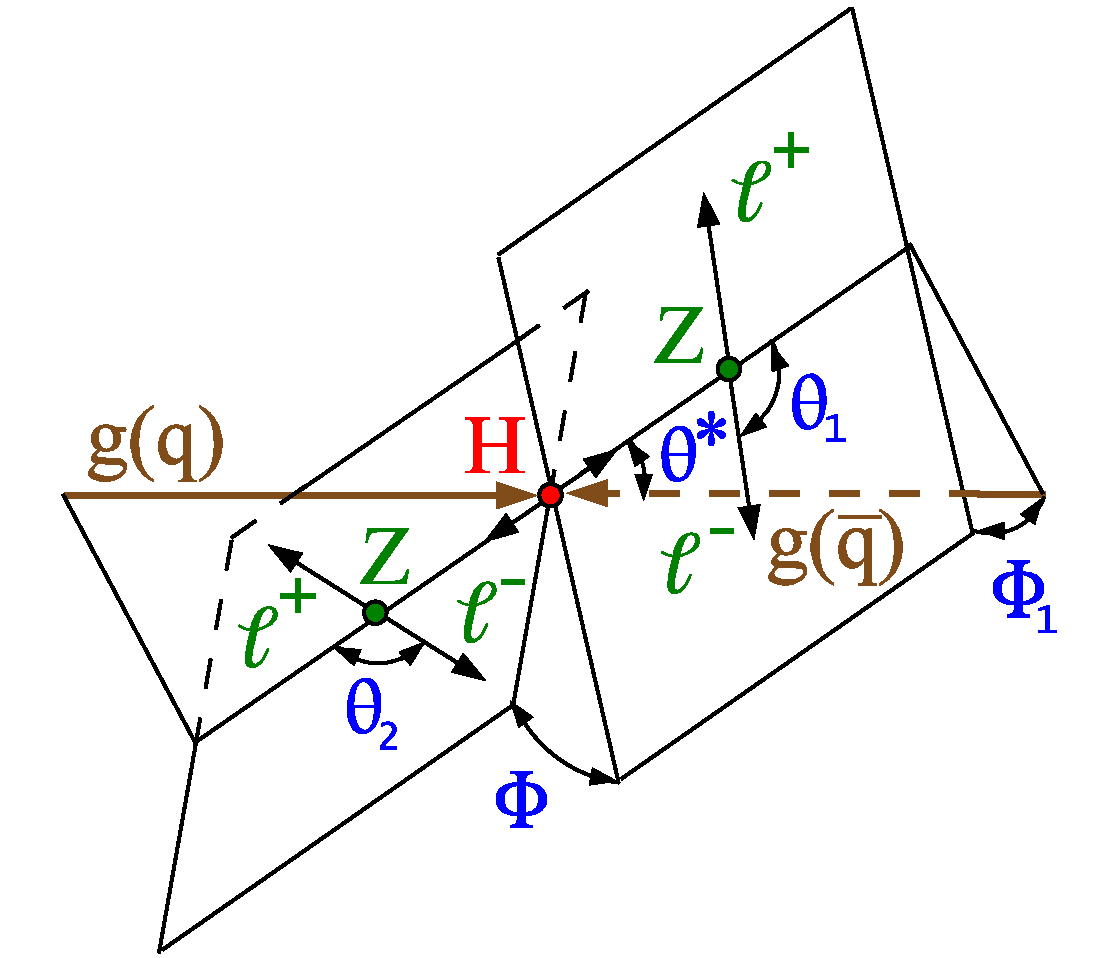
\includegraphics[width=0.57\columnwidth]{Images/H4L/KinematicObservables/angles-h4l.pdf}}
	\caption{Illustration of the $gg/q\bar{q}\to \PH\to ZZ\to 4\ell^\pm$ process. The angular variables reported are considered in the measurements in this analysis. }
	\label{fig:decayHZZ4l}
\end{figure}

The angle $\theta^\star$ is defined as the angle between the beam axis and the direction of the $\PZ_1$ candidate in the event, while $\phi$ and $\phi_1$ are defined as the angles between the three planes containing the \PH boson and the decay products of the $\PZ_1$ and $\PZ_2$ candidates. 
The angles $\theta_1$ and $\theta_2$ are defined as the angles between the $\PZ_1$ and $\PZ_2$ flight directions and the planes containing the di-lepton systems originating from their decay.
In addition, the $\Pp\Pp\to\Hllll$ fiducial cross section is measured in differential bins of the invariant masses of the $\PZ_1$ and $\PZ_2$ candidates.
The set comprising these two observables and the five angles defined above is hereafter referred to as $\vec\Omega^{\HZZfl}\left(\theta^\star,\theta_1,\theta_2,\phi,\phi_1,m_{\PZ_1},m_{\PZ_2}| m_{4\ell}\right)$ and it defines the seven degrees of freedom that completely characterise the $\HZZfl$ process.
The $\vec\Omega^{\HZZfl}$ retains the maximal information present in an event and it can be used to build matrix element discriminants sensitive to the decay of the four lepton final state, as further detailed in Section \ref{sec:discriminants}.

Differential fiducial cross sections are also measured in bins of kinematic observables associated to the jets present in the event, such as: the number of associated jets ($N^{j}$) and the transverse momentum of the leading ($\pt^{j_1}$) and sub-leading ($\pt^{j_2}$) jets.
For events with two or more jets the properties of the di-jet system are assessed by measuring differential cross sections in bins of its invariant mass ($m_{jj}$) and of their differences in pseudorapidity ($\Delta\eta_{jj}$) and azhimutal angle ($\Delta\phi_{jj}$). 
Fiducial cross sections are also measured in bins of smooth functions of the jet rapidity ($\mathcal{T}_{\text{C}}$ and $\mathcal{T}_{\text{B}}$). Thes observables are designed to serve as jet vetoes complementary to $\pt^{j}$ and $N^{j}$ and they are defined as of Ref.~\cite{Gangal:2014qda}:
\begin{linenomath*}
	\begin{equation}
	\label{eqn:tauC}
	\mathcal{T}_{\text{C}} = \max_{j}\left(\frac{\sqrt{E^2_j-p_{z,j}^2}}{2\cosh\left(y_j-Y_\PH\right)}\right),
	\end{equation}
\end{linenomath*}
\begin{linenomath*}
	\begin{equation}
		\label{eqn:tauB}
		\mathcal{T}_{\text{B}} = \max_{j}\left(m^j_{\text{T}}e^{-\mid y_j-Y_\PH\mid}\right),
	\end{equation}
\end{linenomath*}
computed for all the jets in the event and taken from the maximum among them.

The properties of the \PH+jets system are also studied by measuring differential cross sections in bins of the transverse momentum and invariant mass of the four lepton system and the leading jet ($m_{\PH j}$, $\pt^{\PH j}$), or leading and sub-leading jets ($m_{\PH jj}$, $\pt^{\PH jj}$), for events with at least one or two jets, respectively.

%The choice of the bin boundaries for each measurement has been optimised by varying the widths targeting a similar relative uncertainty on the SM expected cross sections in each bin.
%This criterion is found to be equivalent to a definition based on the maximization of the expected discovery significance.

A summary of all the observables considered in this analysis, together with the bin boundaries used for measurements of differential cross sections, is provided in Tab.~\ref{tab:binBoundaries}. The table details also the target of the measurement, specifying wether a given observable is sensitive to the production or the decay of the $\PH\rightarrow 4\ell$ process.
The observables characteristic of the H+j(j) system or the di-jet system can only be defined in events with at least one (or two) jets. In all the other cases, an additional bin containing all the events for which the observable is undefined is introduced in the measurement. This to ensure not only that the integrated cross section corresponds to the SM prediction for the fiducial volume considered in the analysis, but also to account for possible bin-by-bin migrations between generator-level and reconstruction-level events.

\begin{table}[tbp]
	\centering 
	\caption{Variables considered in the analysis and their bin boundaries.}
	\resizebox{\textwidth}{!}{
		\renewcommand{\arraystretch}{1.5}
		\begin{tabular}{lccc}
			Variable & Definition & Bin boundaries & Target \\
			\hline
			$\mH$ &    Invariant mass of the $4\ell$ system       & [105,140] & Inclusive\\
			$\pt^\PH$ & Transverse momentum of the $4\ell$ system  & [0,10,20,30,45,80,120,200,$\infty$) & Production\\
			$|y_\text{H}|$ & Rapidity of the $4\ell$ system  & [0,0.15,0.3,0.6,0.9,1.2,2.5] & Production \\
			$cos \theta^*$ &  Cosine of the decay angle of the leading lepton pair in the $4\ell$ rest frame system  & [0,0.2,0.4,0.6,0.8,1.0] & Decay \\
			$cos \theta_1$, $cos \theta_2$  &  Cosine of the production angle, relative to the $Z$ vector, of the anti-leptons from the two $Z$ bosons & [0,0.2,0.4,0.6,0.8,1.0] & Decay \\
			$\phi$, $\phi_1$ & Azimuthal angles between the decay planes & [0,0,6,1.2,1.8,2.4,3] & Decay \\
			$m_{Z1}$ & Invariant mass of the two leading leptons & [40,65,73,80,85,90,120] & Decay  \\
			$m_{Z2}$ & Invariant mass of the two sub-leading leptons & [12,24,28,32,40,48,65] & Decay \\
			$\pt^{\text{j}_1}$ & Transverse momentum of the leading jet& [0,30,55,95,200,$\infty$) & Production \\
			$\pt^{\text{j}_2}$ & Transverse momentum of the sub-leading jet& [0,30,55,95,200,$\infty$) & Production \\
			$N^{j}$, $N^{j\text{, b-tag}}$&  Number of jets and b-tagged jets& $=$0,$=$1,$=$2,$=$3,$\geq$4 & Event level \\
			$\mathcal{T}_{\text{C}}$, $\mathcal{T}_{\text{B}}$ &  Rapidity weighted jet vetoes & [0,5,10,15,20,25,40,80,$\infty$) & Event level \\
			$m_{jj}$ & Invariant mass of the leading and sub-leading jets system & [120,400,$\infty$) & Production\\
			$\Delta\phi_{jj}$ & Difference in azimuthal angles of the leading and sub-leading jets & $[-\pi,-\pi/2,0,\pi/2,\pi]$ & Production\\
			$\Delta\eta_{jj}$ & Difference in pseudorapidities of the leading and sub-leading jets & [0,0.7,1.6,3.0,10.0] & Production\\
			$\pt^{\PH j}$ & Transverse momentum of the $4\ell$ and leading jet system & [0,60,120,350] & Mixed\\
			$m_{\PH j}$ & Invariant mass of the $4\ell$ and leading jet system & [120,180,220,300,400,600,2000] & Mixed\\
			$\pt^{\PH jj}$ & Transverse momentum of the $4\ell$, leading and sub-leading jets system & [0,60,120,350] & Mixed\\
			$m_{\PH jj}$ & Invariant mass of the $4\ell$, leading and sub-leading jets system & [180,320,450,600,1000,2500] & Mixed\\
		\end{tabular}
	}
	\label{tab:binBoundaries}
\end{table}

A series of double differential cross section measurements is also presented in this analysis with the goal of probing phase space regions of the $\HZZfl$ decay never studied in detail so far in a four-lepton analysis.
%The bins for these measurements are defined with the same approach employed for one dimensional case by adjusting the boundaries targeting a similar relative uncertainty in each bin.
%An example of the bin boundaries adopted for the measurement of the fiducial cross sections in double differential bins of $m_{Z1}$ and $m_{Z2}$ is given in Fig.~\ref{fig:mZ1_mZ2_binning}.
%The boundaries divide the $m_{Z1}$ - $m_{Z2}$ plane in five regions chosen to collect the majority of signal events in two bins, while leaving the most of backgournd event in the other three bins.

%\begin{figure}[tbp]
%	\centering
%	{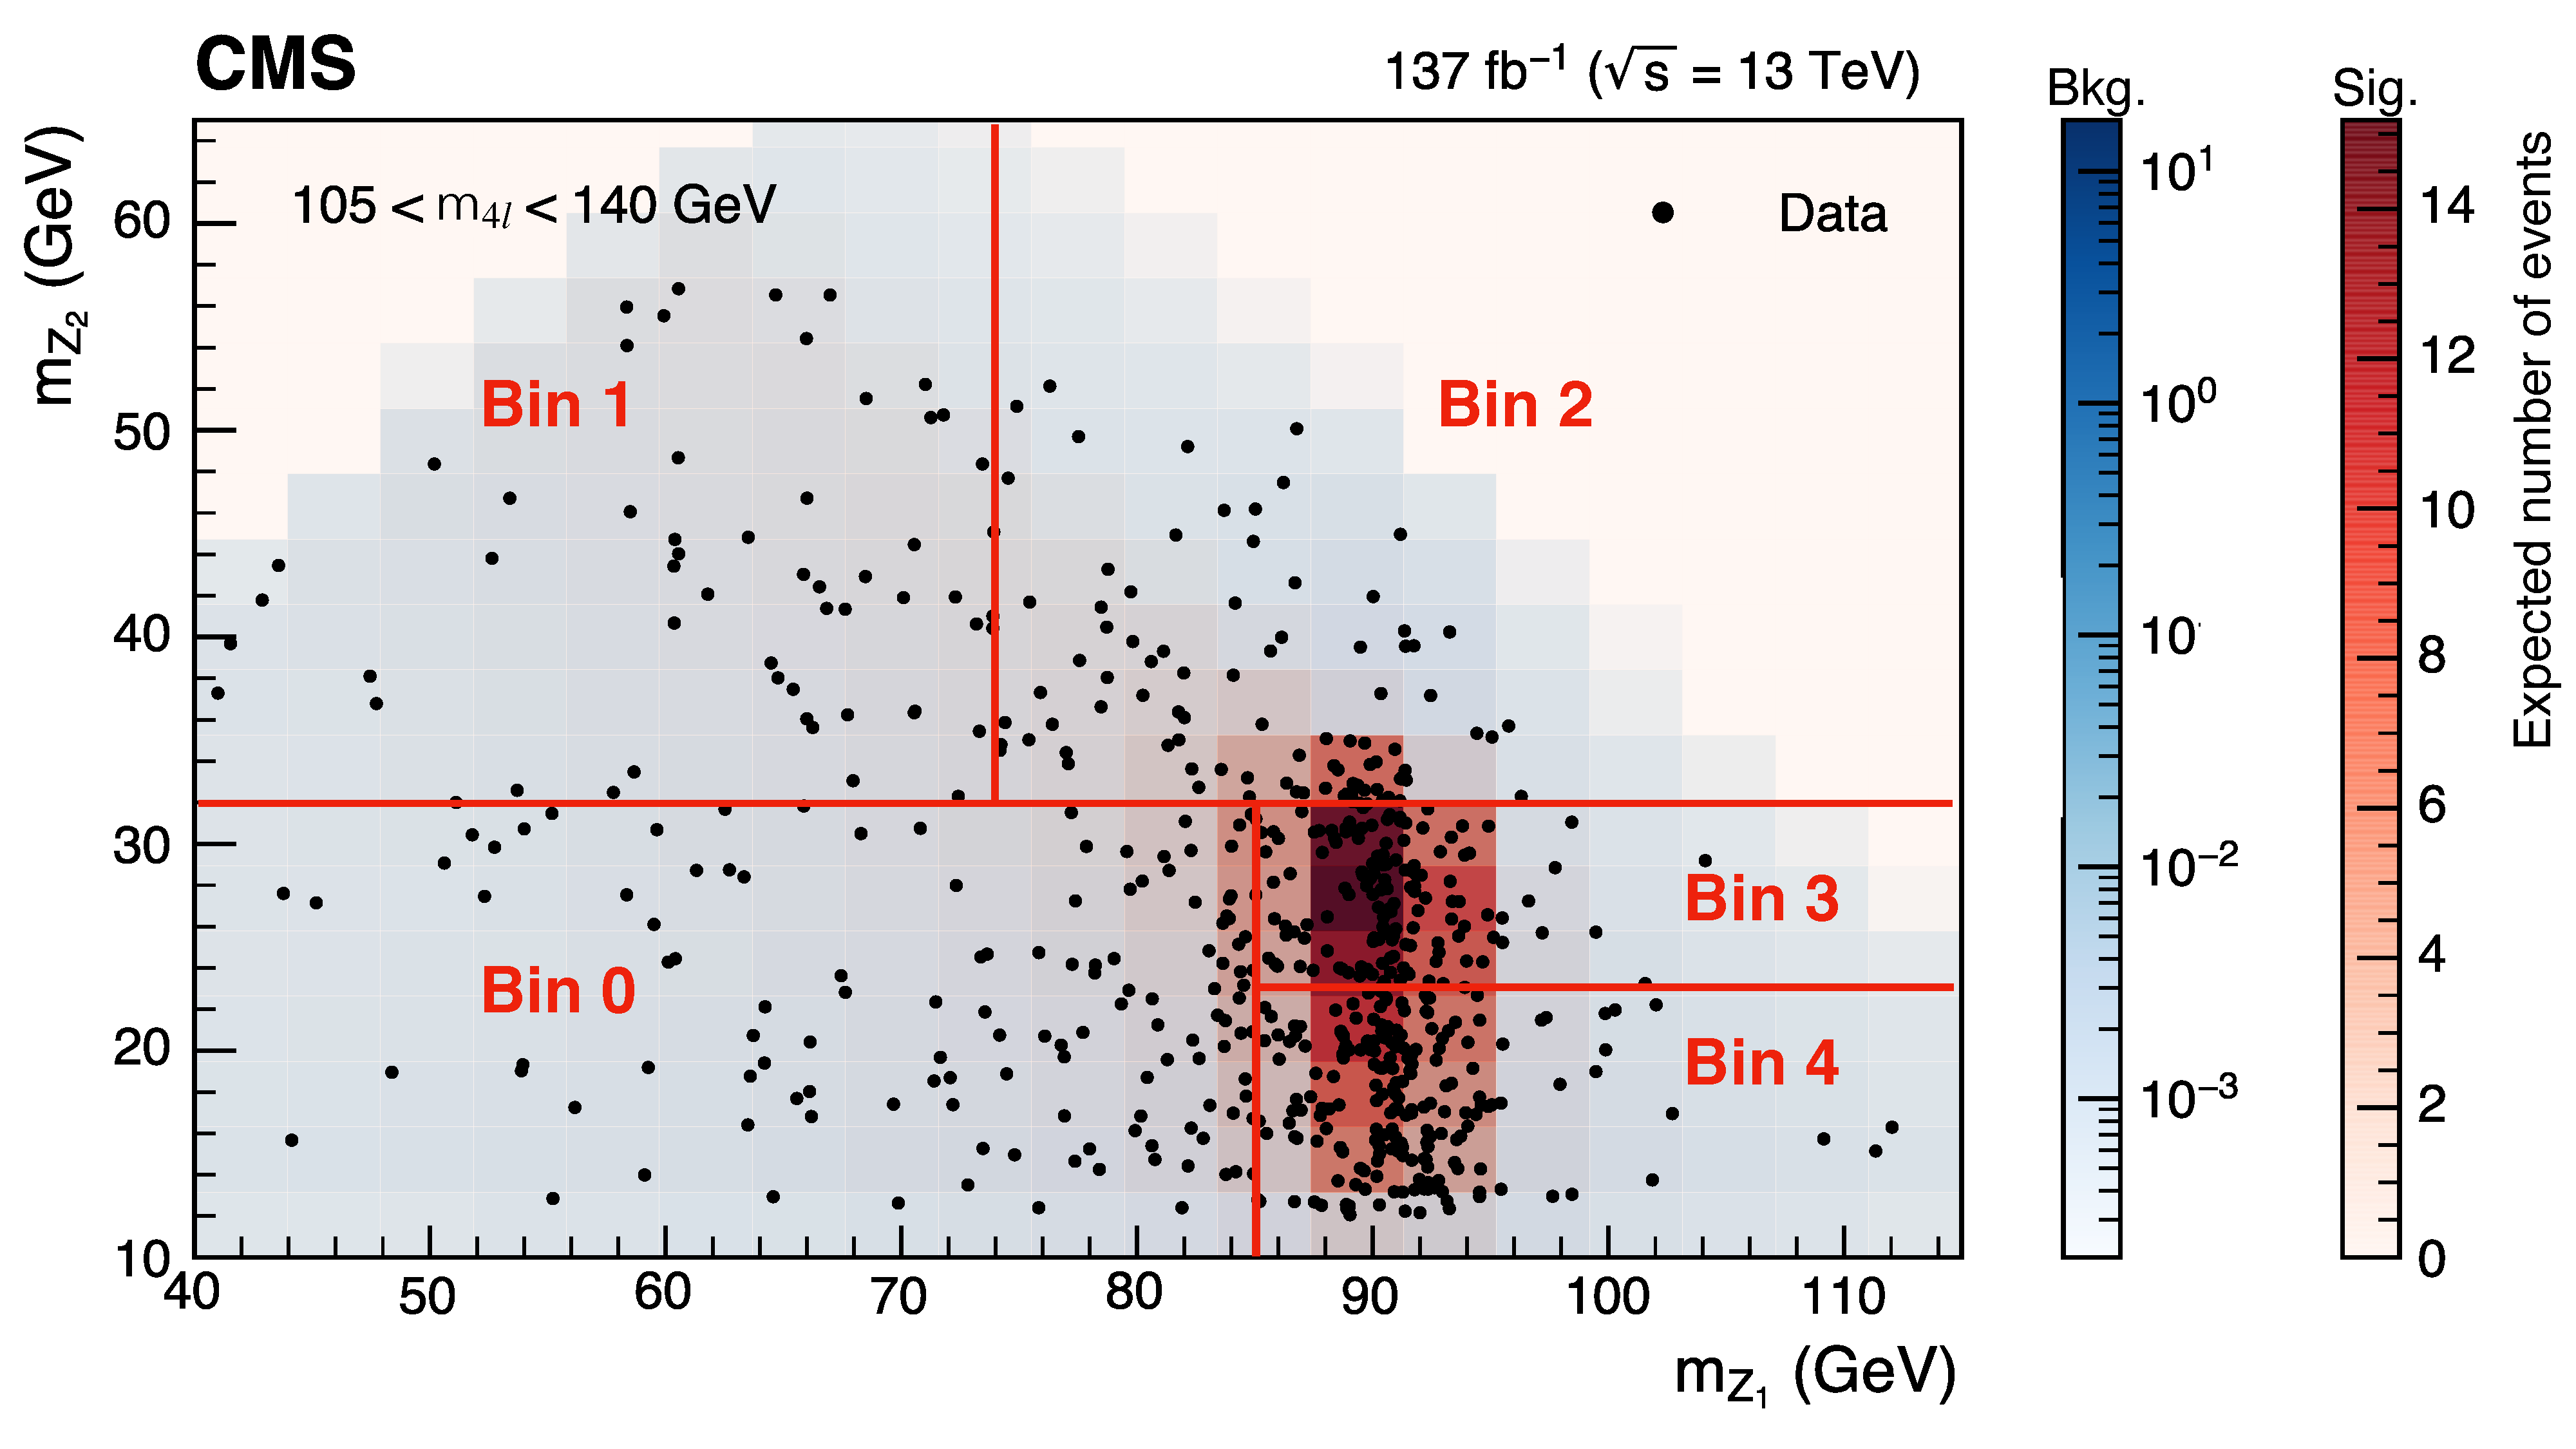
\includegraphics[width=\columnwidth]{Images/H4L/KinematicObservables/mZ1_mZ2_binning}}
%	\caption{Binning for double differential measurement in  $m_{\PZ_{1}}$ - $m_{\PZ_{2}}$.}
%	\label{fig:mZ1_mZ2_binning}
%\end{figure}

The list of the double differential measurements performed in this analysis is reported in Table~\ref{tab:2Dmeasurements},  specifying wether they are sensitive to the production or the decay of the $\PH\rightarrow 4\ell$ process.
The bin boundaries are defined by simultaneous cuts on the two observables that enter the measurement and are detailed for each case separately in Sec.~\ref{sec:results}.

\begin{table}[tbp]
	\centering 
	\caption{Variables considered in the analysis and their bin boundaries.}
	\resizebox{\textwidth}{!}{
		\renewcommand{\arraystretch}{1.5}
		\begin{tabular}{lcc}
			Variable & Definition & Target \\
			\hline
			$\pt^\PH$ vs $|y_\text{H}|$ &  Transverse momentum and rapidity of the 4$\ell$ system & Production\\
			$\pt^\PH$ vs $\mathcal{T}_{\text{C}}$ &  Transverse momentum of the  4$\ell$ system and rapidity-weighted jet veto & Production \\
			$\pt^\PH$ vs $N^{j}$ &  Transverse momentum of the 4$\ell$ system and number of jets in the event  & Production\\
			$m_{\PZ_{1}}$ vs $m_{\PZ_{1}}$ &    Invariant masses of the two $Z$ boson candidates & Decay\\
			$\pt^{j_1}$ vs $\pt^{j_2}$ &  Transverse momenta of the leading and sub-leading jets & Production \\
			$\pt^\PH$ vs $\pt^{\PH j}$ &  Transverse momentum of the 4$\ell$ and 4$\ell$+leading-jet  systems & Production\\
		\end{tabular}
	}
	\label{tab:2Dmeasurements}
\end{table}
%
\subsection{Matrix element discriminants}
\label{sec:discriminants}
The JHUGen and MCFM generators used for the simulation of signal and background events can be used to compute the matrix element probability $\mathcal{P}_a$ for  an event to arise from a physical process $a$, given the value of the reconstructed invariant mass of the four-lepton system $\mllll$, as a function of the set of kinematic observables $\vec\Omega^{\HZZfl}$ defined in Sec.~\ref{sec:observables}.
These probabilities are computed exploiting all the degrees of freedom of the events and therefore retain the maximal information for the description of the underlying physics contained therein.
Hence, the $\mathcal{P}_i(\vec\Omega^{\HZZfl}), i=a,b$ probabilities can be used to construct likelihood-ratio-like matrix element discriminats to discriminate between two physical processes $a$ and $b$, may them be two different production mechanisms of the SM Higgs boson or the test of a BSM hypothesis agains the SM scenario.
This kind of matrix element discriminants has been widely used in the context of the $\HZZfl$ analyses, from the measurement of the $\PH$ boson properties~\cite{CMSHIG19001} up to the constraints on its anomalous couplings~\cite{CMSHIG19009}.
The general structure of these discriminants is an adaptation of the more classic likelihood-ratio, with a slight modification introduced in its definition to make sure that the discriminants are always bounded between 0 and 1.
In general, two different types of kinematic discriminants can be built:
\begin{linenomath}
	\ifthenelse{\boolean{cms@external}}
	{
		\begin{equation}
		\label{eqn:mela}
		\begin{aligned}
		\Dalt &=
		\frac{ \mathcal{P}_{\text{sig}} (\vec\Omega) }
		{\mathcal{P}_{\text{sig}} (\vec\Omega) + \mathcal{P}_{\text{alt}} (\vec\Omega) } \\
		\Dint &=
		\frac{ \mathcal{P}_{\text{int}} (\vec\Omega) }
		{2\cdot\sqrt{\mathcal{P}_{\text{sig}} (\vec\Omega) \cdot \mathcal{P}_{\text{alt}} (\vec\Omega)} },
		\end{aligned}
		\end{equation}
	}
	{
		\begin{equation}
		\label{eqn:mela}
		\begin{aligned}
		\Dalt &=
		\frac{ \mathcal{P}_{\text{sig}} (\vec\Omega) }
		{\mathcal{P}_{\text{sig}} (\vec\Omega) + \mathcal{P}_{\text{alt}} (\vec\Omega) }
		\,\,\,\,\,
		\Dint &=
		\frac{ \mathcal{P}_{\text{int}} (\vec\Omega) }
		{2\cdot\sqrt{\mathcal{P}_{\text{sig}} (\vec\Omega) \cdot \mathcal{P}_{\text{alt}} (\vec\Omega)} },
		\end{aligned}
		\end{equation}
	}
\end{linenomath}

where $\mathcal{P}_{\text{sig}}$ and $\mathcal{P}_{\text{alt}}$ are the SM and BSM probabilities of an event given its kinematic properties in $\vec\Omega$, and $\mathcal{P}_{\text{int}}$ is their interference. 
%These computations rely on the matrix element likelihood apporach implemented in the \textsc{MELA} package~\cite{Gao:2010qx,Bolognesi:2012mm,Anderson:2013afp,Gritsan:2020pib} and exploit the \textsc{jhugen} matrix elements for the signal and the \MCFM matrix elements for the background.

%The full event kinematics is represented by decay observables $\vec\Omega^{\PH\to4\ell}$ that are used to build the set of matrix element discriminant sensitive to the SM \PH boson.
For this analysis a total of six matrix element discriminants, sensitive to different anomalous couplings of the $\PH$ boson, are used to achieve a complete characterisation of the $\PH\to4\ell$ decay.
Tab.~\ref{tab:MEdiscriminants} details the set of kinematic discriminants considered, together with the coupling to which they are sensitive.

\begin{table}[tbp]
	\centering 
	\caption{Matrix element kinematic discriminants considered in the analysis.}
	\renewcommand{\arraystretch}{1.5}
	\begin{tabular}{ ccccc|cc  }
		& \multicolumn{4}{c}{\Dalt}& \multicolumn{2}{c}{\Dint} \\
		\cline{2-7}
		& \multicolumn{6}{c}{Coupling} \\
		& a$_3$ & a$_2$ & $\kappa_1$ & $\kappa_2^{\PZ,\gamma}$ & a$_3$ & a$_2$ \\
		Discriminant & \Dzm & \Dzhp & \DLone & \DLoneZg & \DCP & \Dint \\
	\end{tabular}
	\label{tab:MEdiscriminants}
\end{table}

The $a_i$  and $\kappa_i$ terms correspond to the strengths of vector-boson couplings, following the same notation adopted in Ref.~\cite{CMSHIG19009}.
In particular, the  a$_3$ CP-odd term is expected to be null in the SM and therefore it is sensitive to possible BSM effects that would result in CP violation.
The a$_2$ term correspond to the CP-even contribution to the $\PH\PV\PV$ coupling and it is sensitive to possible BSM contributions from heavy $\PH$ bosons.
The $\kappa_i$ terms are sensitive to possible physics at new energy scale $\Lambda_{1}$ for the VV and the $\PZ \gamma$ couplings respectively.

Differential cross sections are measured in bins of these six matrix element discriminants under the SM hypothesis.
The compatibility of the measurements with the SM predictions is assessed comparing the results with the discriminants built for alternative BSM scenarios, where HVV anomalous couplings of the \PH boson are introduced.

For these observables, as well as for all the ones sensitive to the decay side of the process under study, differential cross sections are measured both for the inclusive $4\ell$ final state and for the $4\Pgm+4\Pe$ and $2\Pe2\Pgm$ final states separately.
This choice is driven by the fact that the same-leptons final states have different physics than the $2\Pe2\Pgm$  final state beacuse of the destructive interference between the two alternative ways of constructing the $\HZZfl$ diagrams in the same-helicity cases.
Presenting the results with this distinction between final states enhances the model-independence of the measurements and widens their possible application, without the need of \textit{ad hoc} assumptions, in their re-interpretations.
%Besides providing the best test statistics to discriminate between two hypotheses, represented by the corresponding probabilities $\mathcal{P}$, the MELA approach is completely reproducible as it relies on phenomenological calculations of the matrix element for the process under study, therefore enhancing the feasibility of \textit{a posteriori} re-interpretations of the results.

\section{Background estimation}
\label{sec:bkgd}

\subsection{Irreducible backgrounds}
\label{sec:irrbkgd}
The irreducible $\PZ\PZ$ background contribution originated from $\Pq\Paq$ annihilation or gluon fusion is estimated from simulation. 
The former is simulated at NLO pQCD with \POWHEG~2.0 and reweighted to NNLO using a K factor computed as a function of $m_{\PZ\PZ}$ exploiting the NNLO computation of the $\qqZZ$ fully differential cross section~\cite{Grazzini2015407}.
The effect of this K factor ranges between 0 and 20\% and is 10\% at $m_{\PZ\PZ}=125\GeV$.
Additional NLO electroweak corrections are extracted from Ref.~\cite{Bierweiler:2013dja} and are applied in the $m_{\PZ \PZ}>2m_{\PZ}$ region depending on the initial state quark flavor and kinematics.

The soft collinear approximation is proven to describe accurately the cross section and the interference term for the gluon fusion $\PZ\PZ$ contribution at NNLO\@~\cite{Bonvini:1304.3053} in pQCD.
In addition, further calculations demonstrate that the K factors are very similar at NLO for signal and background~\cite{Melnikov:2015laa} and at NNLO for signal and interference terms~\cite{Li:2015jva}.
Hence, the same K factor is used for signal and background~\cite{Passarino:1312.2397v1}.
The \textsc{hnnlo}~v2 program~\cite{Catani:2007vq,Grazzini:2008tf,Grazzini:2013mca} is used to obtain the signal NNLO K factor as a function of $m_{\PZ\PZ}$ from the ratio of the NNLO and LO $\Pg\Pg\to\PH\to2\ell2\ell^\prime$ cross sections for the $\PH$ boson decay width of 4.07\MeV. 
The NNLO/LO K factor for {\ggZZ} varies from $\approx$2.0 to 2.6 and is 2.27 at $m_{\PZ\PZ}=125\GeV$, with a 10\% systematic uncertainty for the background process.

%The background processes arising from triboson production $\PZ\PZ\PZ$, $\PW\PZ\PZ$, and $\PW\PW\PZ$, as well as $\ttZ$, $\ttWW$, and $\ttZZ$ are also considered.
%These processes are all estimated from simulation and are referred to as the EW backgrounds in the analysis.

The contribution of these irreducible background processes is included in the form of binned templates in the likelihood function used to extract the differential cross section measurements and it is derived independently in the three final states considered ($4\Pgm$, $4\Pe$, and $2\Pe 2\Pgm$).
The normalisation of these templates is extracted directly from MC, exploiting the most accurate theoretical calculations available to date.
In order to estimate the impact of the theoretical uncertainty on these background normalisations on the inclusive $\Hllll$ fiducial cross section, an additional measurement is performed leaving the normalisation of the irreducible $\PZ\PZ$ processes freely floating in the fit and constraining it through a fit of data in the sidebands of the $\PH$ peak.

\subsection{Reducible background}
\label{sec:redbkgd}
The reducible background contribution to the \PH boson signal in the $4\ell$ channel mainly comes from the $\PZ\text{+jets}$,  $\ttbar\text{+jets}$,
$\PZ\gamma\text{+jets}$, $\PW\PW\text{+jets}$, and $\PW\PZ\text{+jets}$ production, hereafter collectively referred to as $\PZ\text{+jets}$ process.

The contribution from the reducible background is estimated exploiting the same data driven technique emploied in Ref.~\cite{CMSHIG19001} based on lepton misidentification rates and control regions comprising a $\PZ$ candidate and one ($\PZ+\ell$) or two ($\PZ+\ell\ell$) \textit{loose} leptons.

The shapes of the $\PZ\text{+jets}$ reducible background are derived for the three final states ($4\Pgm$, $4\Pe$, and $2\Pe 2\Pgm$) separately and are included as binned templates in the likelihood function used for the statistical analysis.

\section{Signal modelling}
\label{sec:signal}

The parametrization of the $\PH$ resonance as a function of $\mH$ is extracted from a simultaneous fit of signal samples generated at various mass points, following the same approach detailed in Ref.~\cite{CMSHIG19001}.
The normalization of the double-sided Crystal Ball is proportional to $\sigma_{\mathrm{fid}}$, the fiducial cross section and parameter of interest of the analysis.

The shape of the \PH resonant signal, hereafter referred to as $\mathcal{P}(\mllll)$, is described by a double-sided Crystal Ball function~\cite{Oreglia:1980cs} around $\mH \approx 125\GeV$.
The parametrisation of the signal model as a function of $\mH$ is obtained independently for each production mechanism by performing a simultaneous fit of several mass points  in the 105 to 160\GeV mass range.
The non-resonant contribution to the signal in the case of $\WH$, $\ZH$ and $\ttH$ production modes is modelled with the inclusion of a  Landau function in the total probability density function . 
Each parameter of the double-sided Crystal Ball function has a linear dependence on $\mH$, for a total of 12 free parameters.
Fig.~\ref{fig:signal_fit} depicts the results of the fit for the $\ggH$ production mode in the $4\Pe$ and $4\mu$ final states. 

\begin{figure}[!htb]
	\centering
	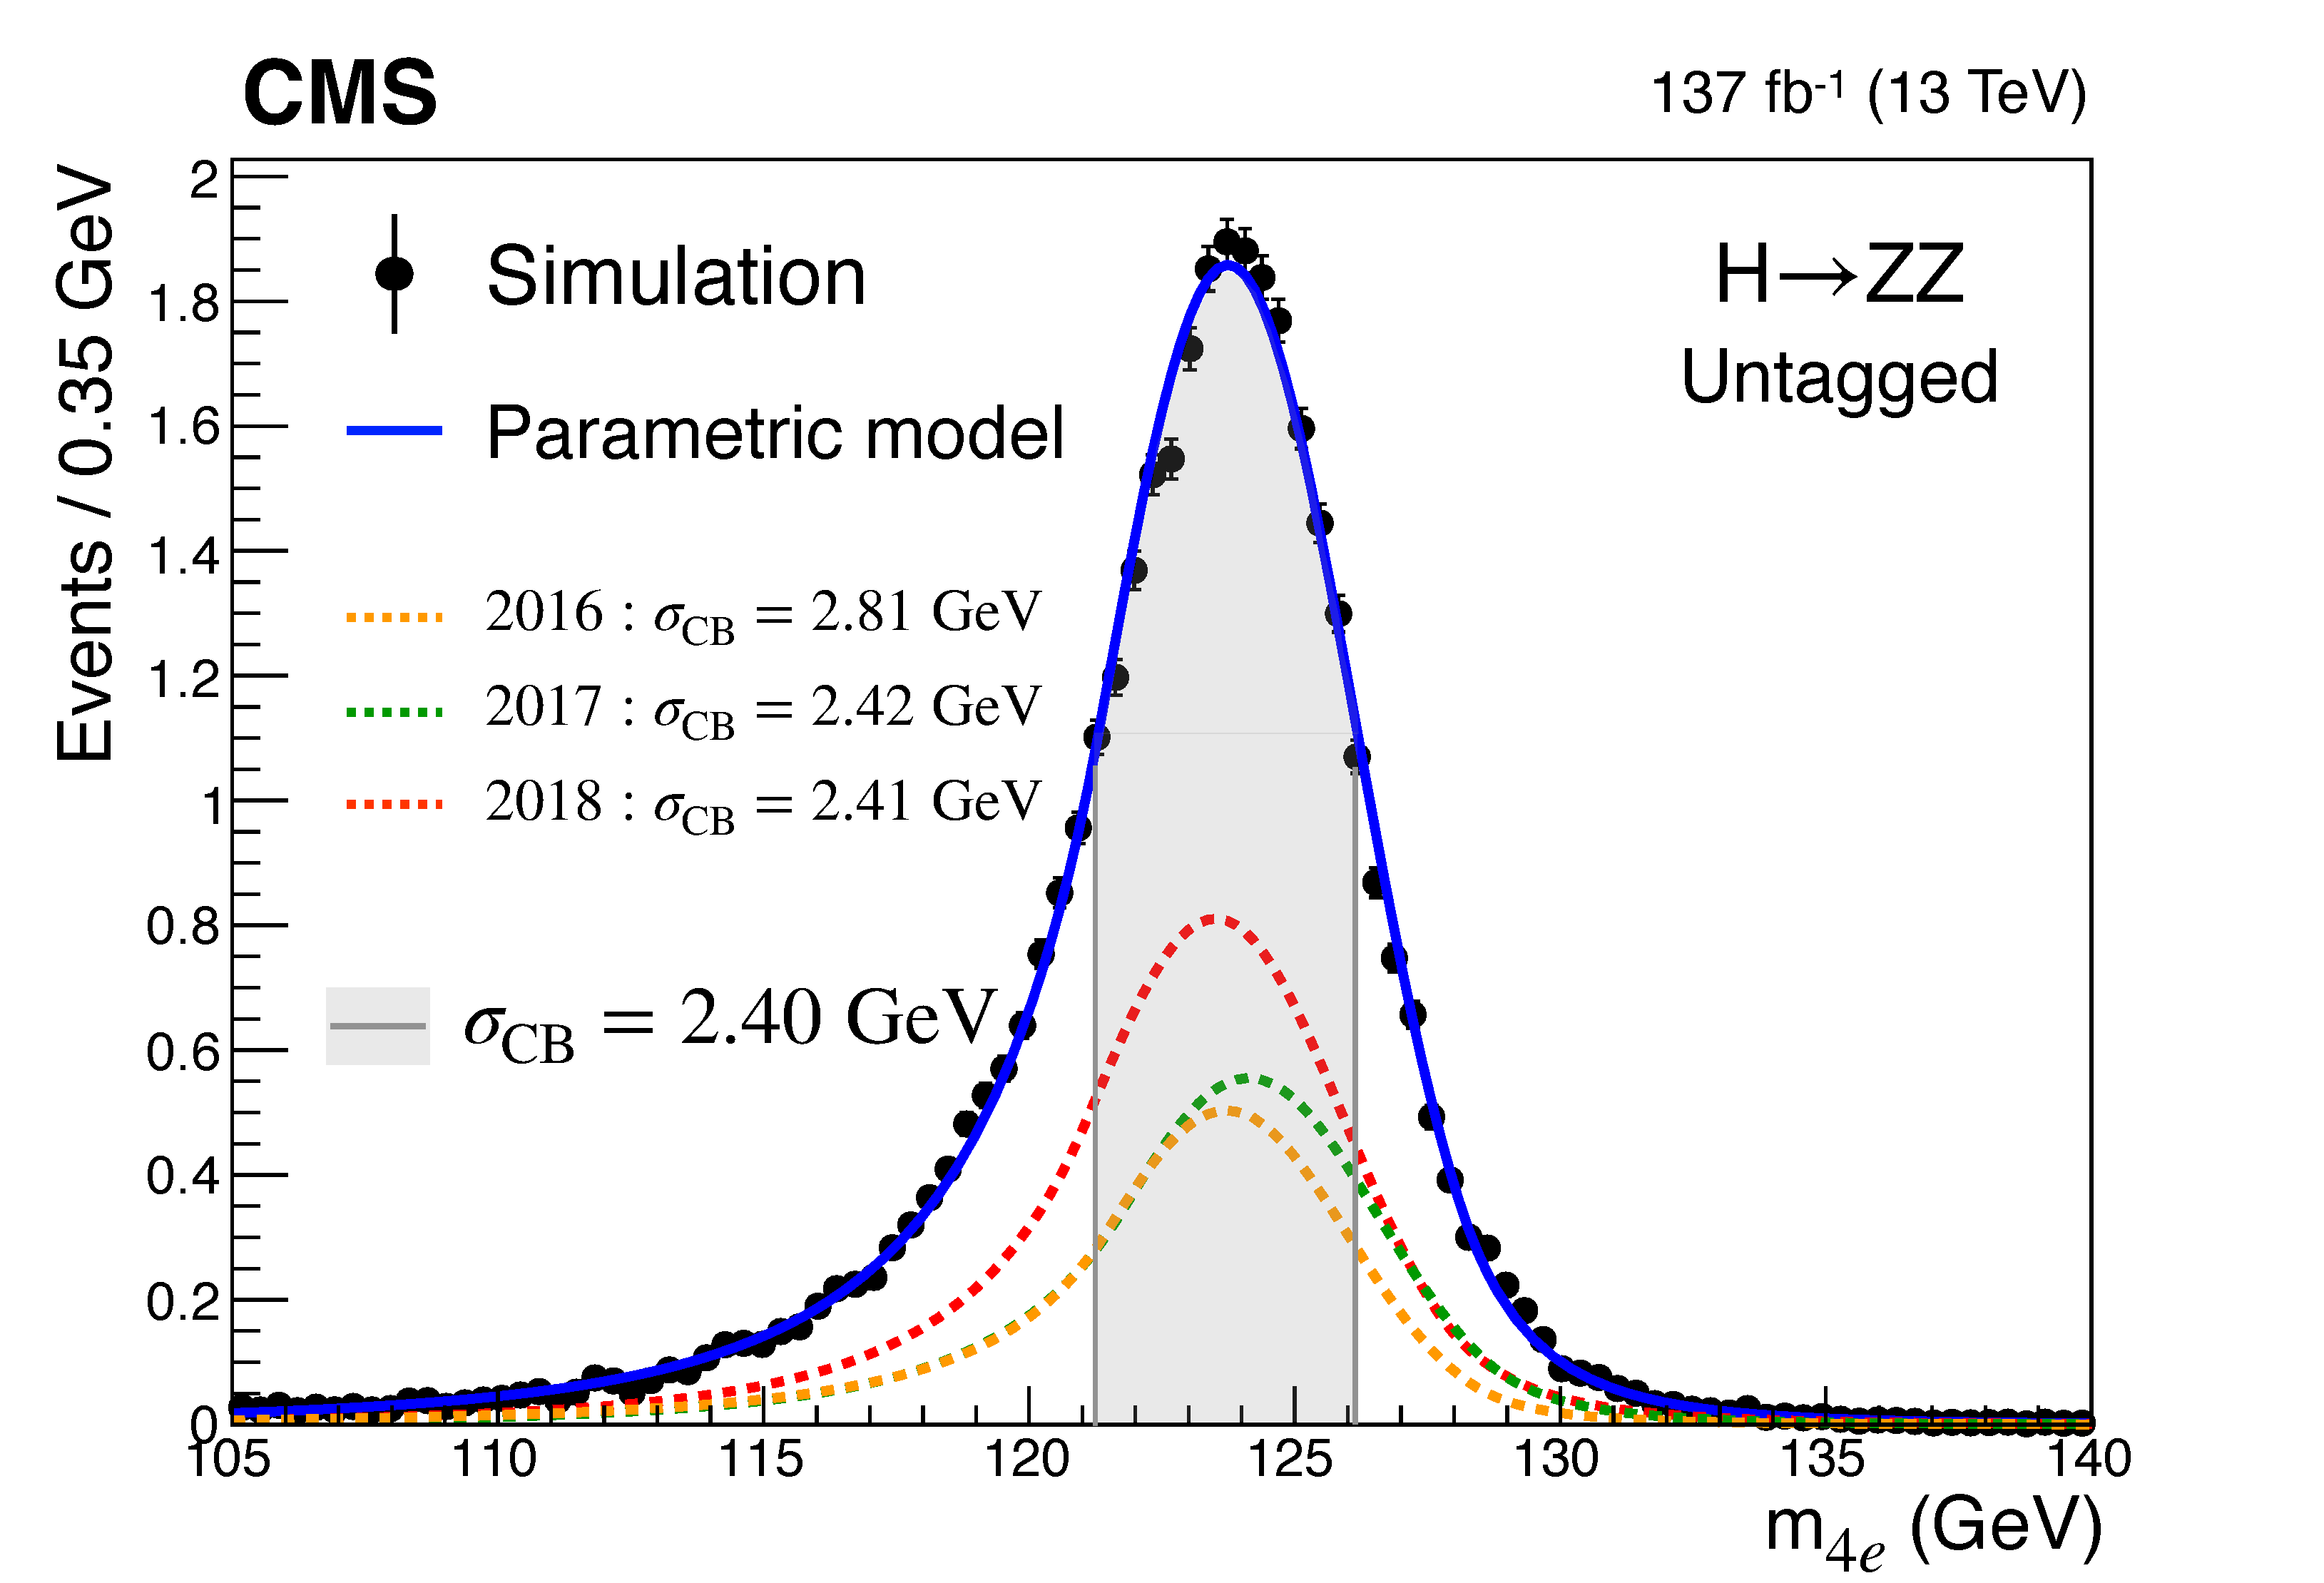
\includegraphics[width=0.49\textwidth]{Images/H4L/Signal/HZZ4e_lineshape.pdf}
	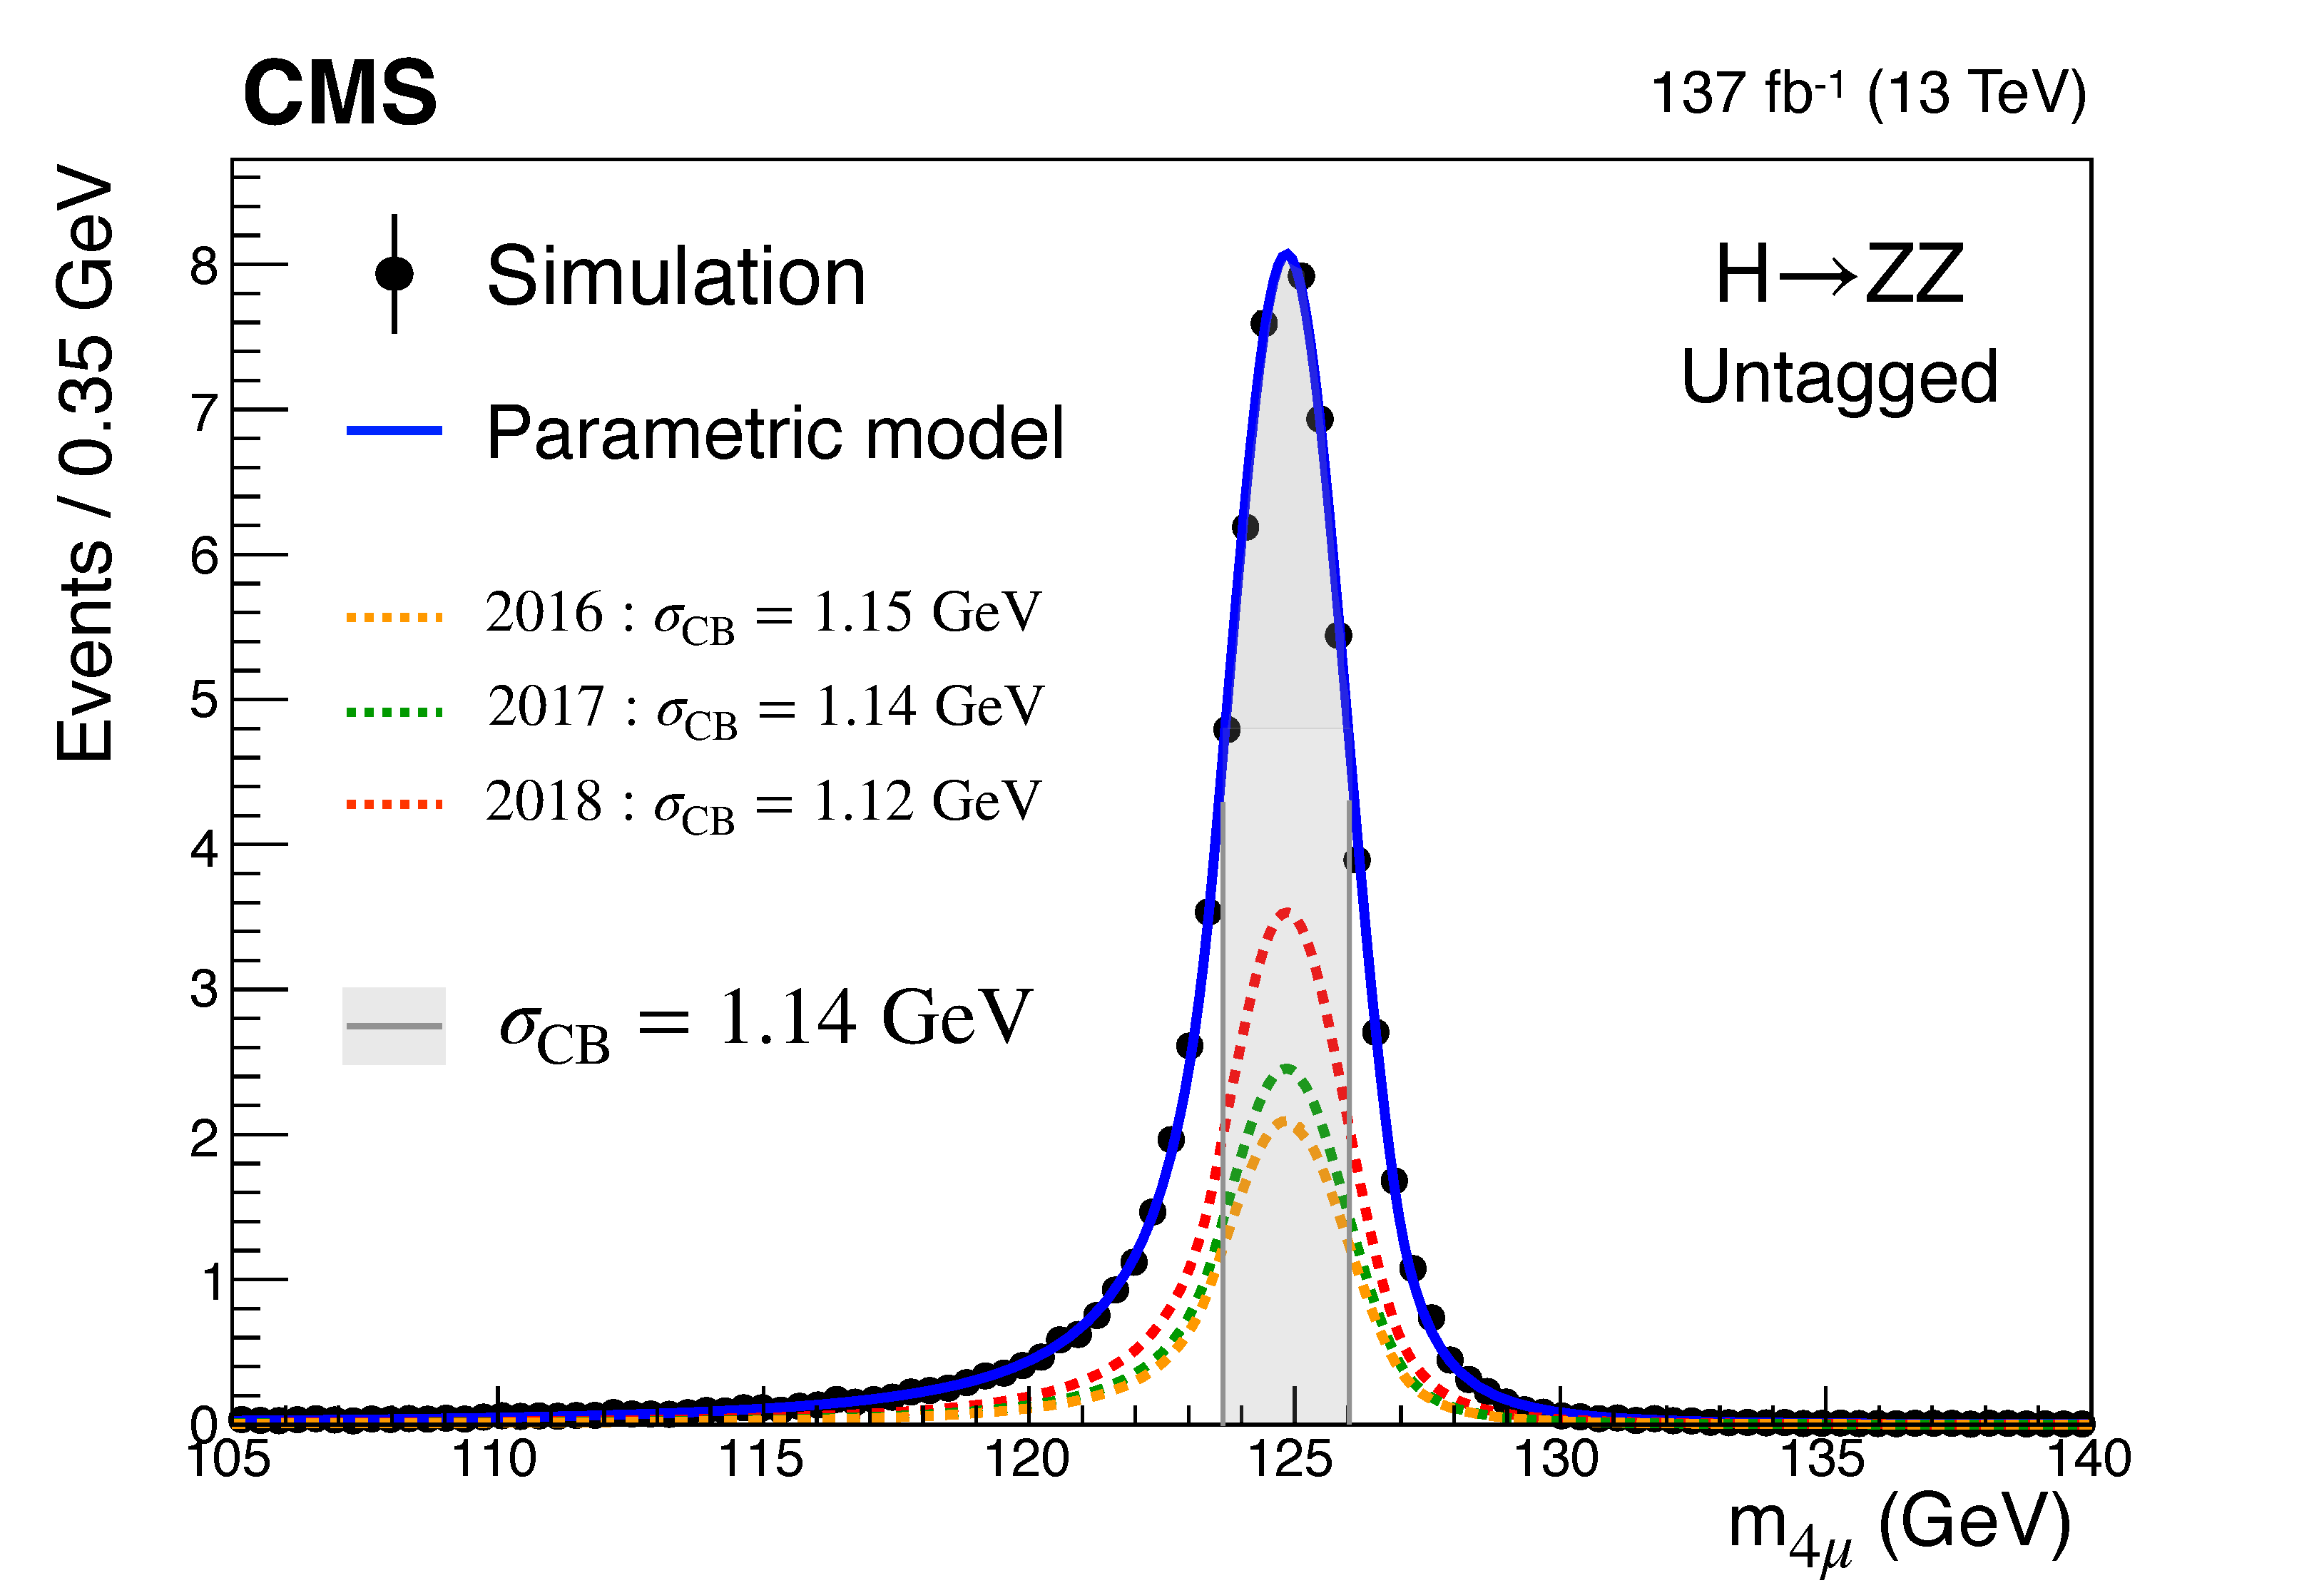
\includegraphics[width=0.49\textwidth]{Images/H4L/Signal/HZZ4mu_lineshape.pdf}
	\caption{
% 		\textcolor{red}{\textbf{EDIT, TAKEN FROM 19001}}
		The shape of the parametric signal model for each year of simulated data, and for the sum of all years together.
		The black points represent weighted simulation events of the $\ggH$ production mechanism for $\mH=125\GeV$ and the blue line the corresponding model.
		Also shown is the $\sigma_{\text{CB}}$ value (half the width of the narrowest interval containing 68\% of the invariant mass distribution) in the gray shaded area.
		The contribution of the signal model from each year of data-taking is illustrated with the dotted lines.
		The models are shown for the $4\Pe$ (\cmsLeft) and $4\Pgm$ (\cmsRight) final states in the untagged event category.
		\label{fig:signal_fit}}
\end{figure}

\section{Measurement methodology}
\label{sec:measurement}

The $\Pp\Pp\to\Hllll$ cross section is measured within a fiducial volume defined as detailed in Section \ref{sec:fiducialvolume}.
%The integrated fiducial cross section is measured as well as differential cross sections as a function of several kinematic observables sensitive to both the production and the decay sides of the $\Pp\Pp\to\Hllll$ process. 
%In order to enhance the sensitivity to specific phase space regions and probe in more detail the SM predictions, double differential cross section measurements are also performed.
%The SM predictions for the \PH boson decay into four lepton are tested against different BSM scenarios by measuring cross sections in differential bins of the matrix element kinematic discriminants introduced in Section~\ref{sec:discriminants}.

The measurements are extracted by means of a maximum likelihood fit of the signal and background distributions to the observed $4\ell$
mass distribution, $N_{\mathrm{obs}}(\mllll)$, defined in each final state $f$ and in each bin $i$ of a given observable as:

\begin{linenomath}
	\ifthenelse{\boolean{cms@external}}
	{
		\begin{equation}
		\label{eqn:m4l}
		\begin{aligned}
		N_{\mathrm{exp}}^{f,i}(m_{4\ell}) &= N_{\mathrm{fid}}^{f,i}(m_{4\ell})+N_{\mathrm{nonfid}}^{f,i}(m_{4\ell})+N_{\mathrm{nonres}}^{f,i}(m_{4\ell})\\
		&+N_{\text{bkg}}^{f,i}(m_{4\ell}) \\
		&=\sum_j\epsilon_{i,j}^{f}  \left(1+f_{\mathrm{nonfid}}^{f,i} \right)\sigma_{\mathrm{fid}}^{f,j}  \mathcal{L}\mathcal{P}_{\mathrm{res}}(m_{4\ell}) \\
		&\,\,\,+ N_{\mathrm{nonres}}^{f,i}\mathcal{P}_{\mathrm{nonres}}(m_{4\ell})+N_{\text{bkg}}^{f,i}\mathcal{P}_{\text{bkg}}(m_{4\ell}).
		\end{aligned}
		\end{equation}
	}
	{
		\begin{equation}
		\label{eqn:m4l}
		\begin{aligned}
		N_{\mathrm{exp}}^{f,i}(m_{4\ell}) &= N_{\mathrm{fid}}^{f,i}(m_{4\ell})+N_{\mathrm{nonfid}}^{f,i}(m_{4\ell})+N_{\mathrm{nonres}}^{f,i}(m_{4\ell})+N_{\text{bkg}}^{f,i}(m_{4\ell}) \\
		&=\sum_j\epsilon_{i,j}^{f}  \left(1+f_{\mathrm{nonfid}}^{f,i} \right)\sigma_{\mathrm{fid}}^{f,j}  \mathcal{L}\mathcal{P}_{\mathrm{res}}(m_{4\ell}) \\
		&\,\,\,+ N_{\mathrm{nonres}}^{f,i}\mathcal{P}_{\mathrm{nonres}}(m_{4\ell})+N_{\text{bkg}}^{f,i}\mathcal{P}_{\text{bkg}}(m_{4\ell}).
		\end{aligned}
		\end{equation}
	}
\end{linenomath}

The resonant signal contribution is parametrized with a double-sided Crystal Ball function, $\mathcal{P}_{\mathrm{res}}(m_{4\ell})$, with a normalization coefficient proportional to the fiducial cross section, $\sigma_{\mathrm{fid}}$.
The results of the fit are extracted as signal strength modifiers by measuring the ratio of $\sigma_{\mathrm{fid}}$  observed in a given fiducial bin to the corresponding SM expectation.
A Landau distribution is introduced to model empirically the shape of the non-resonant signal contribution, $\mathcal{P}_{\mathrm{nonres}}(m_{4\ell})$, for the $\WH$, $\ZH$, and $\ttH$ processes where one of the leptons from the \PH boson decay is either not selected or falls out of the acceptance.
The shape parameters of the Landau distribution are constrained in the fit to be within a range determined from simulation.
These non-resonant events form what is referred to in the analysis as ``combinatorial signal'' and are treated as a background in the measurement.

{\tolerance=800 Detector effects unavoidably introduce differences between the observables used for the fiducial phase space definition and the corresponding quantities at the reconstruction level. 
An additional contribution ($f_{\mathrm{nonfid}}$) is introduced to take into account the presence of events not originating from the fiducial volume but selected for the analysis and it is treated as background in the measurements.
This contribution is referred to as the ``non-fiducial signal'' and it is estimated from simulation for each of the signal models studied.
Dedicated studies on simulation have shown the shape of these events is identical to the shape of the resonant fiducial signal. To minimise the model dependence of the measurement, the value of $f_{\mathrm{nonfid}}$ is fixed to be a fraction of the fiducial signal component.
The values of this fraction are reported in Tab.~\ref{tab:summarySM} and have been found to range between 5\% for the $\ggH$ production mechanism up to 18\% for the $\ttH$ mode.\par}

The quantity $\epsilon_{i,j}^{f}$ represents the detector response matrix that is used to unfold the number of expected events in bin \textit{i} at the reconstruction level to the number of expected events in bin \textit{j} of a given observable at the fiducial level.
Simulated signal samples are used to determine the response matrix, which is also corrected for residual differences between data and simulation.
The measurement of the integrated fiducial cross section is performed within a single bin ($105<\mllll<160\GeV$) and therefore the response matrices become single numbers, listed in Table~\ref{tab:summarySM} for different SM production mechanism.

The table shows also the acceptance $\mathcal{A}_{\mathrm{fid}}$, defined as the fraction of signal events that fall within the fiducial phase space.
%The fraction of signal events within the acceptance of the fiducial phase space, $\mathcal{A}_{\mathrm{fid}}$, and the reconstruction efficiency, $\epsilon$, for the different production mechanisms of the \PH boson are listed in Tab.~\ref{tab:summarySM}. 
%The table also shows the fraction of resonant signal events that do not originate from the fiducial phase space, $f_{\mathrm{nonfid}}$.
%All these quantities, along with the $(1+f_{\mathrm{nonfid}})\epsilon$ factor, are further described in Section~\ref{sec:measurement}.
%It is worth noting the relatively weak dependence of the $(1+f_{\mathrm{nonfid}})\epsilon$ factor on the \PH boson production mechanism resulting from the definition of the fiducial phase space volume and therefore ensuring the model independence of the measurements.

\begin{table*}[!h!tb]
	\centering
	\topcaption{
% 		\textcolor{red}{\textbf{EDIT CAPTIONS, NUMBERS ALREADY UP TO DATE}}
		Summary of the fraction of signal events for different SM signal production modes within the fiducial phase space (acceptance $\mathcal{A}_{\mathrm{fid}}$),
		reconstruction efficiency ($\epsilon$) for signal events in the fiducial phase space,
		and ratio of the number of reconstructed events outside the fiducial phase space to that of the reconstructed events in the fiducial phase space ($f_{\mathrm{nonfid}}$).
		For all production modes the values given are for $\mH = 125\GeV$.
		Also shown in the last column is the factor $(1+f_{\mathrm{nonfid}})\epsilon$ which regulates the signal yield for a given fiducial cross section.
		The uncertainties listed are statistical only. The theoretical uncertainty in $\mathcal{A}_{\mathrm{fid}}$ for the SM is less than 1\%.
		\label{tab:summarySM}
	}
	\begin{tabular}{lcccc}
		Signal process & $\mathcal{A}_{\mathrm{fid}}$ & $\epsilon$ & $f_{\mathrm{nonfid}}$  & $(1+f_{\mathrm{nonfid}})\epsilon$ \\
		\hline
		$\ggH$ (\POWHEG) & 0.408 $\pm$ 0.001 & 0.619 $\pm$ 0.001 & 0.053 $\pm$ 0.001 & 0.652 $\pm$ 0.001 \\
		$\VBF$ & 0.448 $\pm$ 0.001 & 0.632 $\pm$ 0.002 & 0.043 $\pm$ 0.001 & 0.659 $\pm$ 0.002 \\
		$\WH$ & 0.332 $\pm$ 0.001 & 0.616 $\pm$ 0.002 & 0.077 $\pm$ 0.001 & 0.664 $\pm$ 0.002 \\
		$\ZH$  & 0.344 $\pm$ 0.002 & 0.626 $\pm$ 0.003 & 0.083 $\pm$ 0.002 & 0.678 $\pm$ 0.003 \\
		$\ttH$ & 0.320 $\pm$ 0.002 & 0.614 $\pm$ 0.003 & 0.179 $\pm$ 0.003 & 0.725 $\pm$ 0.005 \\
	\end{tabular}
\end{table*}

The systematic uncertainties described in Section~\ref{sec:systematics} are included in the form of nuisance parameters (NPs) and the fiducial cross section measurements are obtained using an asymptotic approach~\cite{LHC-HCG} with a test statistic based on the profile likelihood ratio~\cite{Cowan_2011}.
The maximum likelihood fit is performed simultaneously in all final states and in all bins of the observable under study, assuming a \PH boson mass $\mH=125.38\GeV$.
The branching fractions of the \PH boson to different final states ($4\Pe,4\Pgm,2\Pe2\Pgm$) are left floating in the fit in order to increase the model independence of the measurements, following the same strategy of Ref.~\cite{CMSHIG19001}.
A likelihood-based unfolding procedure is performed to resolve detector effects from the observed distributions to the fiducial phase space. 
This approach is the same as in
Refs.~\cite{Khachatryan:2015yvw}, \cite{CMSHggFiducial8TeV}, and \cite{CMSHIG19001} and it has the advantage of performing simultaneously the unfolding of the detector effects and the likelihood fit to extract the fiducial cross section.
The analysis strategy of Ref.~\cite{CMSHIG19001} is extended here by measuring also double differential cross sections and by measuring the fiducial cross sections in $4\Pgm+4\Pe$ and $2\Pe 2\Pgm$ final states separately when observables targeting the $\Hllll$ decay are considered.
When these measurements are performed, the branching fractions of the \PH boson decay are fixed to the SM expectation.

\section{Systematic uncertainties}
\label{sec:systematics}
The integrated luminosities of the 2016, 2017, and 2018 data-taking periods are individually known with uncertainties in the 1.2--2.5\% range~\cite{CMS-PAS-LUM-17-001,CMS-PAS-LUM-17-004,CMS-PAS-LUM-18-002}, while the total Run~2 (2016--2018) integrated luminosity has an uncertainty of 1.6\%, the improvement in precision reflecting the (uncorrelated) time evolution of some systematic effects. 

Experimental systematic uncertainties due to the trigger and the lepton reconstruction and selection efficiencies are estimated from data for the different final states. 
This uncertainties range from 0.8 to 1.9\% in the 4\Pgm channel and from 6.5 to 11\% in the 4\Pe channel.
Compared to Ref.~\cite{CMSHIG19001} a reduction of about 5\% in the 4\Pe uncertainties has been achieved thanks to a dedicated method introduced in the analysis.
The large difference still present between the two final states reflects the usage of a low mass di-muon resonance for the estimation of the 4\Pgm uncertainties in the low $\pt^{\Pgm}$ regions, whereas only the \PZ boson resonance can be exploited in the 4\Pe channel, yielding to larger uncertainties in the low $\pt^{\Pe}$ region.


{\tolerance=800 The systematic uncertainties on the lepton momentum scale and resolution are estimated from dedicated studies on the $\Zll$ mass distribution in data and simulation.
The scale uncertainty is found to be 0.04\% in the 4\Pgm channel and 0.3\% in the 4\Pe channel, while the resolution uncertainty is 20\% for both channels.
The effect of these uncertainties in introduced in the analysis by floating the corresponding parameters of the double-sided Crystal Ball function used to model the resonant signal as described in Sec.~\ref{sec:signal}.\par} 

Systematic uncertainties on the jet energy scale and smearing are considered when dealing with measurements involving jet-related observables, as they can introduce migrations around the different bin boundaries.
These uncertainties are considered to act on the normalisation of the processes and are modelled with a set of 22 NPs following the central CMS recommendations, taking into account partial correlations among the different sources of uncertainty that impact on the jet energy scale and smearing.
%They can also alter the shape of the discriminants, but the effect on the shape is negligible.

%A systematic uncertainty on the {\PQqb}-tagging efficiency is introduced in the analysis for the measurment of the differential cross section as a function of the number of {\PQqb}-tagged jets.

Experimental systematic uncertainties on the reducible background estimation, described in Section~\ref{sec:redbkgd}, are also considered.
These originate from the background composition and misidentification rate uncertainties vary between 30 and 45\% depending on the final state.
However, the impact of this uncertainty on the measurements is found to be negligible.

Theoretical uncertainties on the renormalization and factorization scales, and the choice of the PDF set affect both the signal and the background rates.
The QCD uncertainty from the renormalization and factorization scales is determined by varying these scales between 0.5 and 2 times their nominal value, while keeping their ratio between 0.5 and 2.
The uncertainty due to the PDF set is determined following the PDF4LHC recommendations by taking the root mean square of the variation of the results when using different replicas of the default NNPDF set~\cite{Botje:2011sn,Alekhin:2011sk}.
An additional 10\% uncertainty in the K factor used for the $\ggZZ$ prediction is applied as described in Section~\ref{sec:irrbkgd}.
A systematic uncertainty of 2\%~\cite{deFlorian:2016spz} in the branching fraction of $\Hllll$ only affects the signal yield.

\section{Results}
\label{sec:results}

\subsection{Inclusive cross section}
The integrated fiducial cross section for the $\HZZfl$ process is measured to be
$$\obsXSECFid$$ at $\mH = 125.38\GeV$
and it is found to be in good agreement with the SM expectation of $\sigma_{{\mathrm{fid}}}^{\mathrm{SM}}=\expXSECFid$, as shown by the corresponding log-likelihood scan in Fig.~\ref{fig:fiducial_LLScan}.
The inclusive fiducial cross section measured in the three final states considered in this analysis ($4\Pgm,\,4\Pe,\,$ and $2\Pe 2\Pgm$)  is shown in the left panel of Fig.~\ref{fig:fiducial_inclusive}, while the right panel depicts the evolution of the $\HZZfl$ fiducial cross section as a function of the center of mass energy.
The results are compared with the cross sections predicted by the POWHEG and NNLOPS generators for the \PH boson production and parton showering, while the decay is always modelled by the JHUGen generator.
In addition to what presented in Ref.~\cite{CMSHIG19001}, the results are also compared with the predictions from the MADGRAPH5\_aMC@NLO generator.
A summary of the measurement is presented in Table~\ref{tab:fiducial_inclusive}, together with a breakdown of the uncertainties into its statistical and systematic components and the results for each individual data taking period analysed.

%%%%%%%%%%%%%%%%%%%%%% Inclusive Fiducial XSEC %%%%%%%%%%%%%%%%%%%%%%

\begin{figure}[!htb]
	\centering
	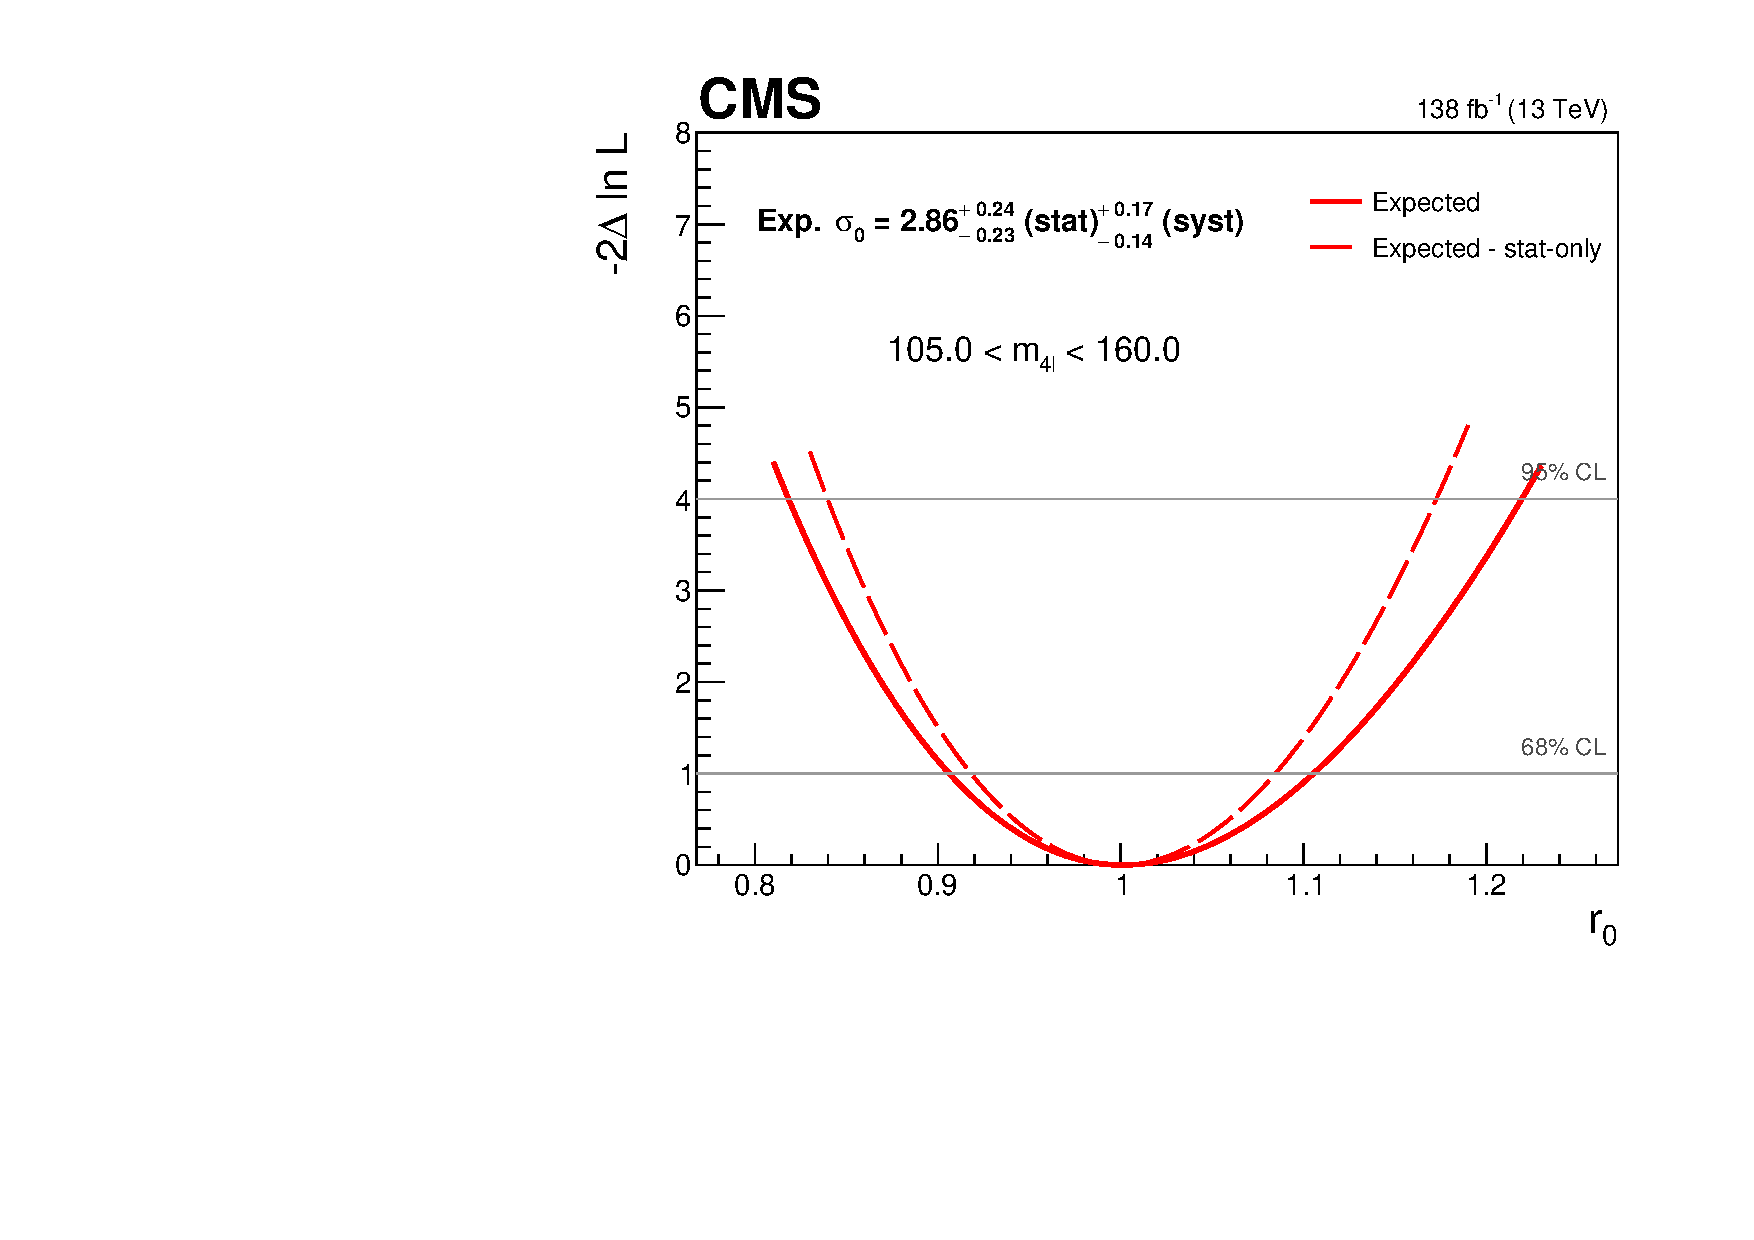
\includegraphics[width=0.5\textwidth]{Images/H4L/lhscan_compare_mass4l_SigmaBin0.pdf}
	\caption{
		Log likelihood scan for the measured inclusive fiducial cross section measurement.
		\label{fig:fiducial_LLScan}}
\end{figure}

\begin{figure}[!htb]
	\centering
	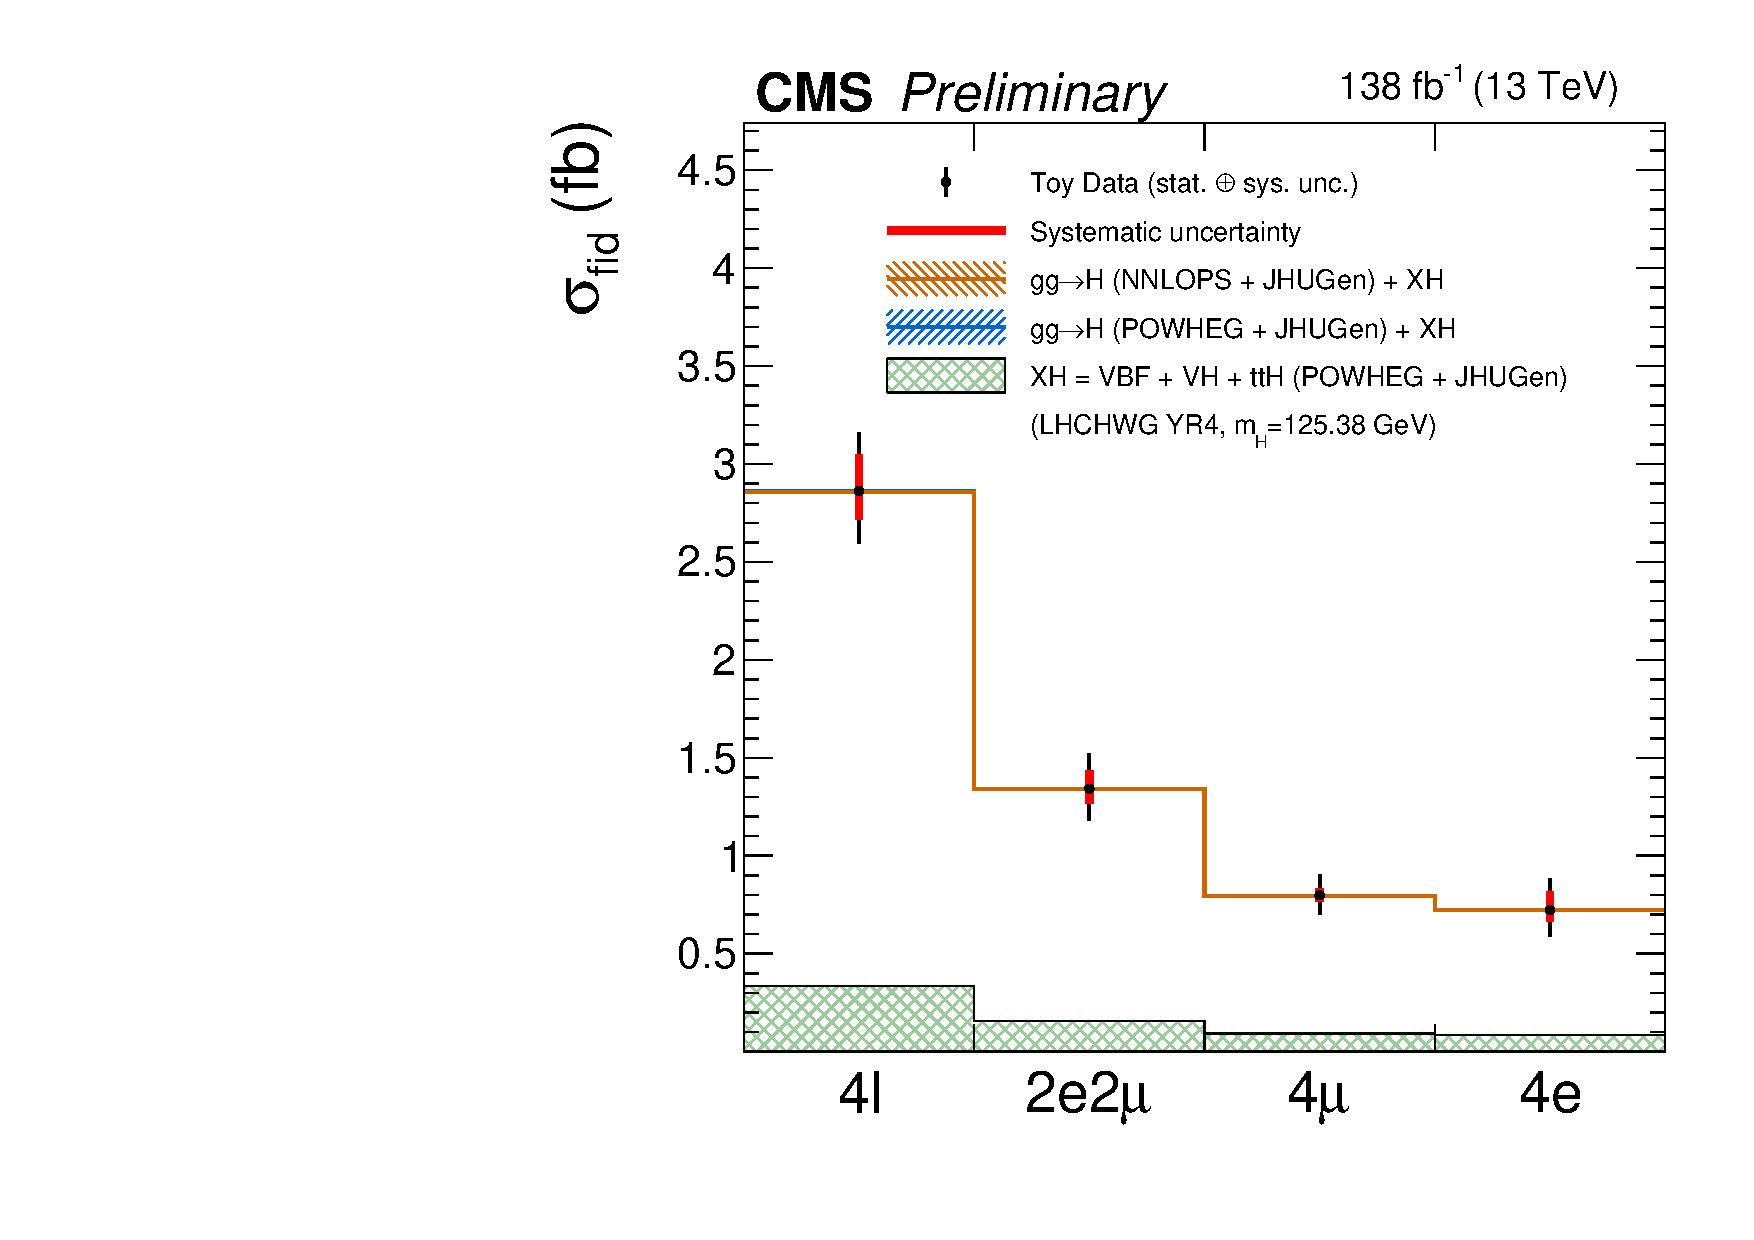
\includegraphics[width=0.48\textwidth]{Images/H4L/mass4l_unfoldwith_SM_125_asimov.pdf}
	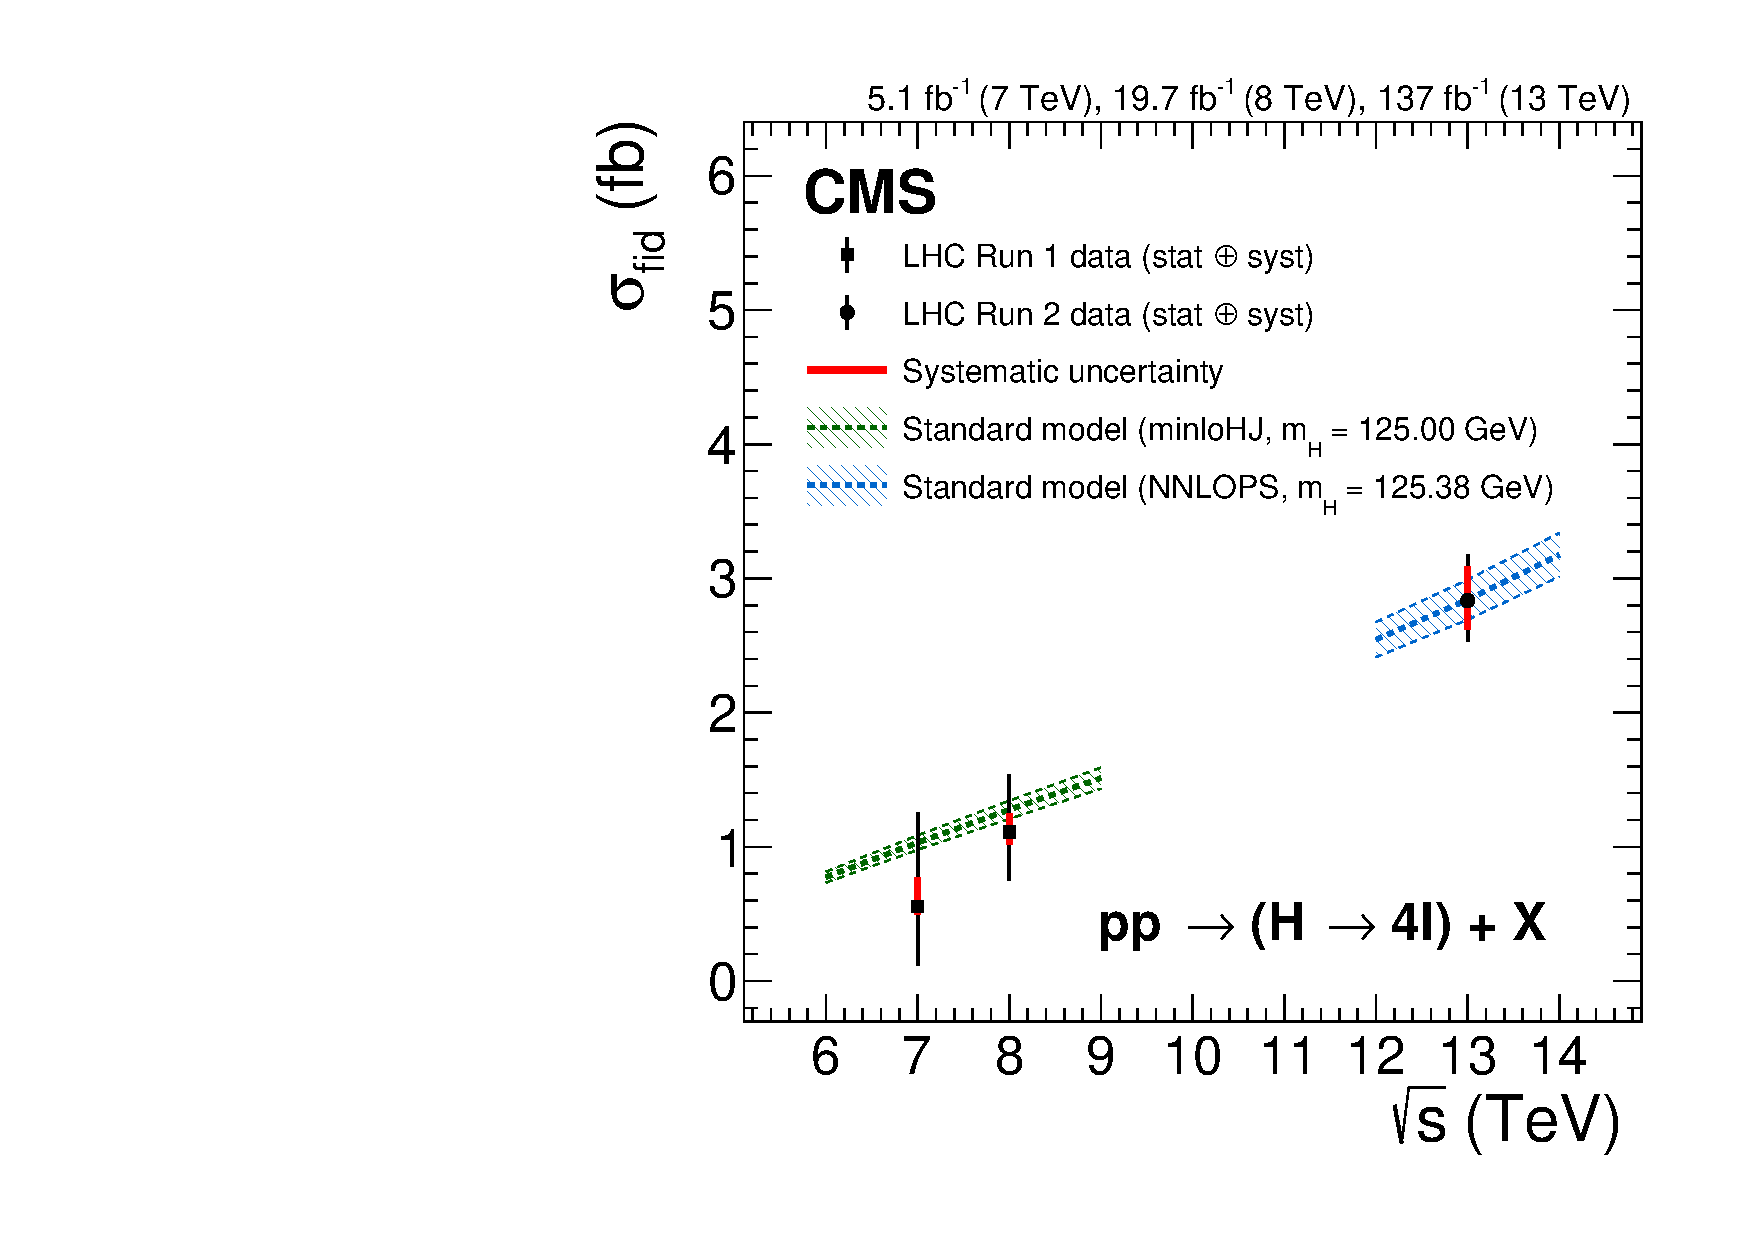
\includegraphics[width=0.48\textwidth]{Images/H4L/Figure_016-b.pdf}
	\caption{
		The measured inclusive fiducial cross section in different final states (\cmsLeft) and integrated as a function of $\sqrt{s}$ (\cmsRight).
		The acceptance is calculated using \POWHEG at  $\sqrt{s}=13\TeV$ and \textsc{HRes}~\cite{Grazzini:2013mca,deFlorian:2012mx}
		at $\sqrt{s}=$~7 and 8\TeV.
		\label{fig:fiducial_inclusive}}
\end{figure}

\begin{table*}[!htb]
	\centering
	\topcaption{
		The measured inclusive fiducial cross section and $\pm 1$ standard deviation uncertainties for different final states and data-taking periods at $\mH=125.38 \GeV$.
		The statistical and systematic uncertainties are given separately for the inclusive measurements.
		\label{tab:fiducial_inclusive}
	}
	\renewcommand{\arraystretch}{1.5}
	\begin{tabular}{ccccc}
		& $2\Pe 2\Pgm$~(fb) & $4\Pgm$~(fb) & $4\Pe$~(fb) & Inclusive (fb) \\
		\hline
		2016 & $X^{+Y}_{-Z}$ & $X^{+Y}_{-Z}$ & $X^{+Y}_{-Z}$ & $X^{+Y}_{-Z} = A\stat+B\syst$  \\
		2017 & $X^{+Y}_{-Z}$ & $X^{+Y}_{-Z}$ & $X^{+Y}_{-Z}$ & $X^{+Y}_{-Z} = A\stat+B\syst$   \\
		2018 & $X^{+Y}_{-Z}$ & $X^{+Y}_{-Z}$ & $X^{+Y}_{-Z}$ & $X^{+Y}_{-Z} = A\stat+B\syst$   \\
		2016--2018 & $1.34^{+0.18}_{-0.17}$ & $0.80^{+0.10}_{-0.10}$ & $0.72^{+0.16}_{-0.13}$ & $\obsXSECFid$   \\
	\end{tabular}
\end{table*}

%%%%%%%%%%%%%%%%%%%%%% Inclusive Fiducial XSEC: Float ZZ norm %%%%%%%%%%%%%%%%%%%%%%

The measurement of the inclusive fiducial cross section is repeated floating the normalisation of the \PZ\PZ$^\star$ irreducible background processes considered.
As explained in Sec.~\ref{sec:irrbkgd}, the normalisation of these processes is taken from MC simulation after applying dedicated scale factors to account for  NLO corrections in the theory predictions.
These corrections come with an associated uncertainty that may be reduced by a dedicated measurement of this normalisation using sidebands in data.
In addition, floating the normalisation of the irreducible background processes may enhance the model independence of the analysis.
The results are presented in Fig.~\ref{fig:fiducial_zzfloating} for the inclusive $\Hllll$ measurement as well as for the three final states considered. Fig.~\ref{fig:fiducial_zzfloating_corr} presents the corresponding correlation matrices.

\begin{figure}[!htb]
	\centering
	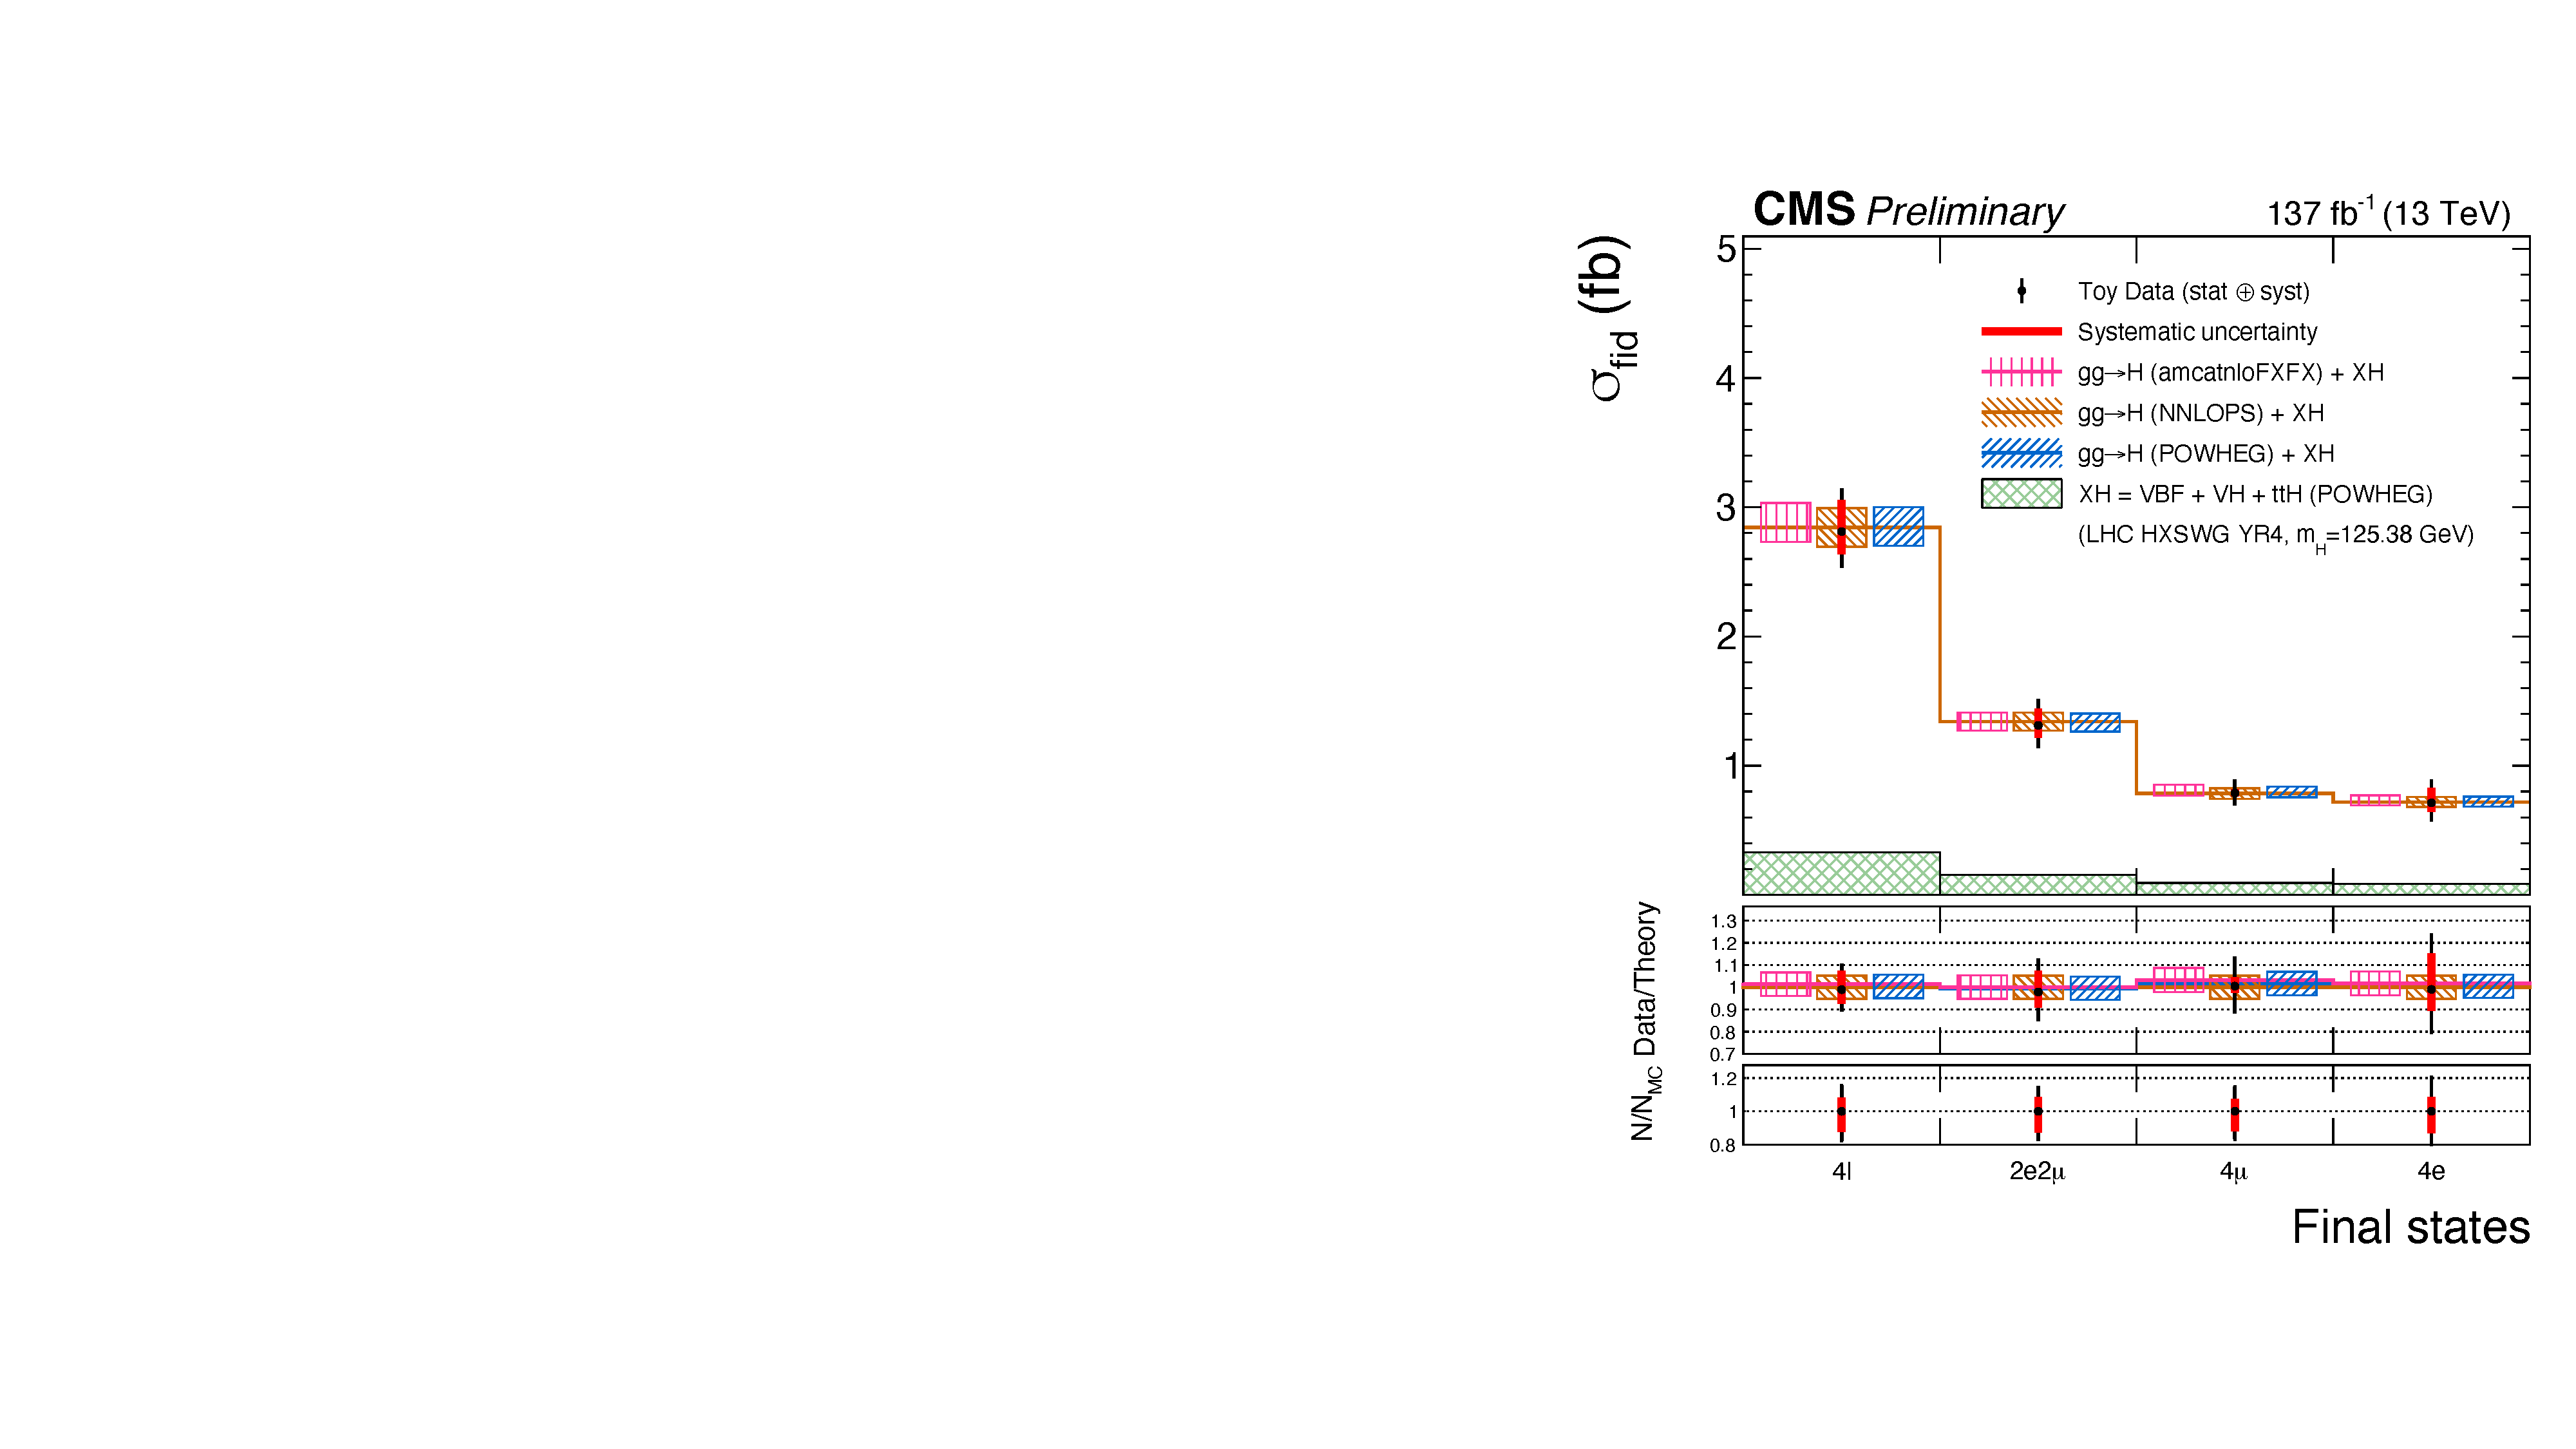
\includegraphics[width=0.5\textwidth]{Images/H4L/zznorm/mass4l_zzfloating_unfoldwith_SM_125_asimov_v1.pdf}
	\caption{
		The inclusive fiducial cross section measured in different final states with the irreducible backgrounds normalisation \PZ\PZ$^\star$  floating in the fit.
		The acceptance and theoretical uncertainties in the differential bins are calculated using the \POWHEG (blue), NNLOPS (orange), and MadGraph\_aMC@NLO (pink) generators.
        The sub-dominant component of the signal ($\VBF + \VH + \ttH$) is denoted as XH and it is fixed to the SM.
        The ratio to the theoretical prediction obtained from each generator is shown in the central panel, while the bottom panel shows the ration between the measured \PZ\PZ$^\star$ normalisation and the prediction from MC.
		\label{fig:fiducial_zzfloating}}
\end{figure}

\begin{figure}[!htb]
	\centering
	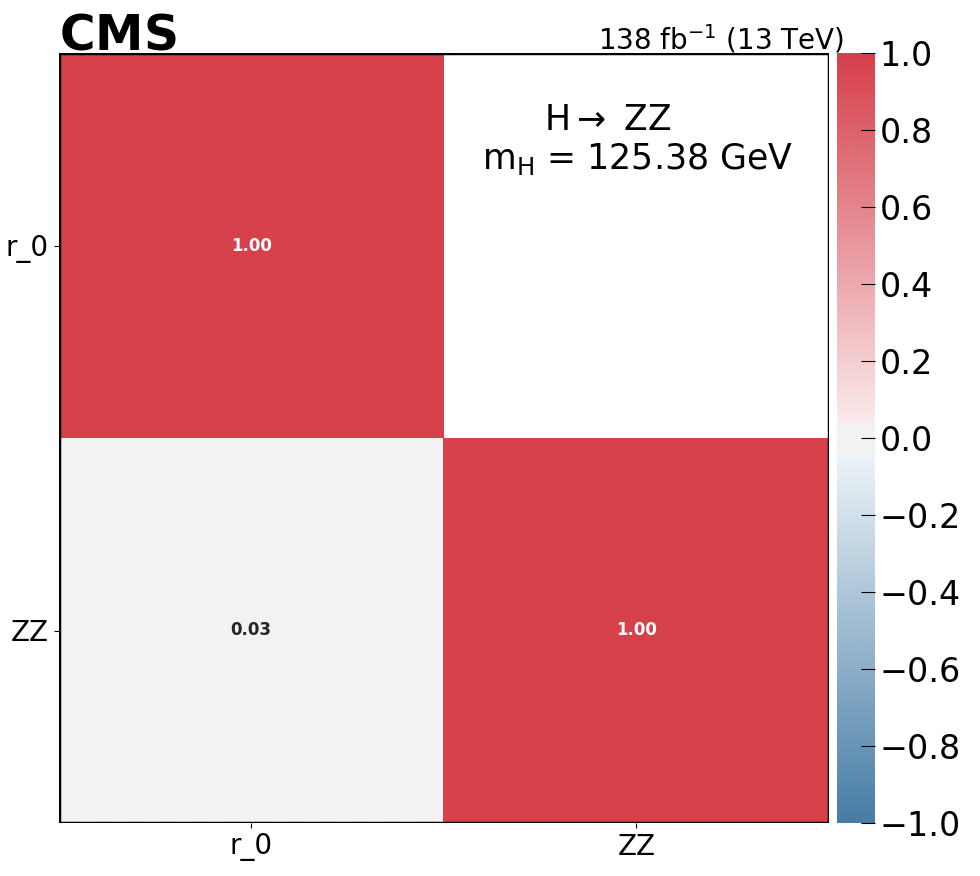
\includegraphics[width=0.48\textwidth]{Images/H4L/zznorm/corr_m4l_v3.png}
	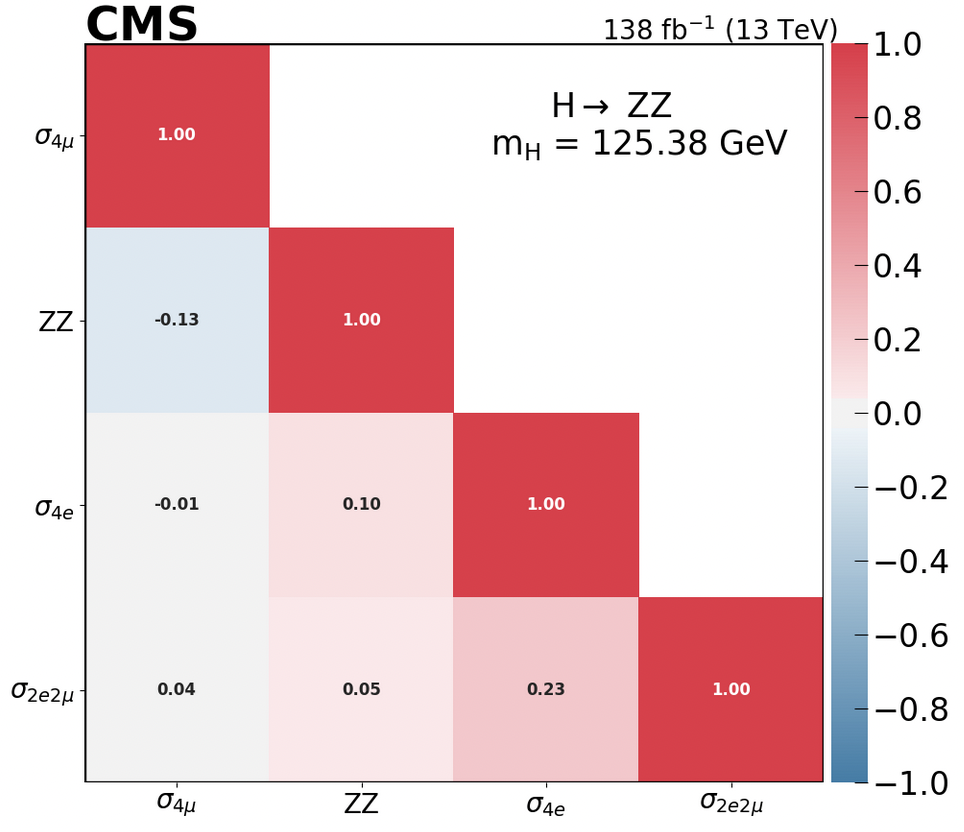
\includegraphics[width=0.48\textwidth]{Images/H4L/zznorm/corr_m4l_v2.png}
	\caption{
		Correlation matrices between the inclusive fiducial cross section and the \PZ\PZ$^\star$ normalisation (left). Correlations between the fiducial cross sections in each final state and the \PZ\PZ$^\star$ normalisation (right).
		\label{fig:fiducial_zzfloating_corr}}
\end{figure}


Tab.~\ref{tab:fiducial_zzfloat} summarises the measured cross sections and \PZ\PZ$^\star$ normalisation.
No large correlation is observed between the different fiducial cross sections and the \PZ\PZ$^\star$ normalisation.
The measured cross sections are found to be in agreement with the results obtained when the irreducible background normalisation is extracted from MC simulation and fixed to the SM expecation in the measurement.
In addition, the uncertainty on this parameter, when it is extracted from a fit of the data sidebands, is found to be larger than the theoretical uncertainty on its predictions.
For all these reasons, in the following the \PZ\PZ$^\star$ normalisation is taken from MC without introducing any model depdence or worsening of the analysis performance.

\begin{table*}[!htb]
	\centering
	\topcaption{
		The measured inclusive fiducial cross section and $\pm 1$ standard deviation uncertainties for different final states and data-taking periods at $\mH=125.38 \GeV$.
		The statistical and systematic uncertainties are given separately for the inclusive measurements.
		\label{tab:fiducial_zzfloat}
	}
	\renewcommand{\arraystretch}{1.5}
	\begin{tabular}{ccccc}
		& $2\Pe 2\Pgm$~(fb) & $4\Pgm$~(fb) & $4\Pe$~(fb) & Inclusive (fb) \\
		\hline
		$\sigma_{{\mathrm{fid}}} $& $1.34^{+0.18}_{-0.16}$ & $0.80^{+0.11}_{-0.10}$ & $0.72^{+0.16}_{-0.14}$ &  $2.86^{+0.23}_{-0.22}\stat^{+0.18}_{-0.15}\syst \unit{fb}$  \\
		 \PZ\PZ$^\star$ norm. & $410^{+40}_{-50}$ & $410^{+40}_{-50}$ & $410^{+40}_{-50}$ & $410^{+40}_{-50}$   \\
	\end{tabular}
\end{table*}

\clearpage

\subsection{Differential cross sections: production}
Fiducial cross sections are measured in differential bins of variables sensitive to the production side in the $\HZZfl$ channel.
The results for the transverse momentum and rapidity of the Higgs boson are shown in Fig.~\ref{fig:fidPTH},\ref{fig:fidYH}, respectively.
Fig.~\ref{fig:fidNJ},\ref{fig:fidPTJ1},\ref{fig:fidPTJ2} show the measurements of the fiducial cross sections in differential bins of jet-related observables, namely: the number of associated jets in the event and the transverse momentum of the leading and sub-leading jet in the event.
The fiducial cross section is also measured in bins of the inveriant mass of the dijet system, as shown in Fig.~\ref{fig:fidMJJ}. This measurement, performed for the first time in the $4\ell$ channel, allows to enhance the sensitivity of the analysis to phase space regions of $\VBF$ and $\ttH$ production mechanisms, where a larger jet-multiplicity is expected.

This analysis presents also the results for the cross sections measured in bins of observables of the \PH+j and \PH+jj systems. These results meet the constantly increasing interest from the theory community, as they allow to probe the QCD emission pattern with experimental data.
The measurements of the fiducial cross section in differential bins of the invariant mass and transverse momentum of the \PH+j system are presented in Fig.~\ref{fig:fidMHJ} and \ref{fig:fidPTHJ}, respectively, while Fig.~\ref{fig:fidPTHJJ} shows the results in differential bins of the transverse momentum of the \PH+jj system.

With the same goal of enhancing the sensitivity to phase space regions that probe directly the departure from LO kinematics and thus the QCD emission pattern, the cross sections in differential bins of the rapidity-weighted jet-vetoes introduced in Sec.~\ref{sec:observables} are also measured. Fig.~\ref{fig:fidTC} presents the results for  $\mathcal{T}_{\text{C}}$, while the results for  $\mathcal{T}_{\text{B}}$ are shown in Fig.~\ref{fig:fidTB}.

\clearpage

\begin{center}
	\begin{figure}[!htbp]
		\centering
		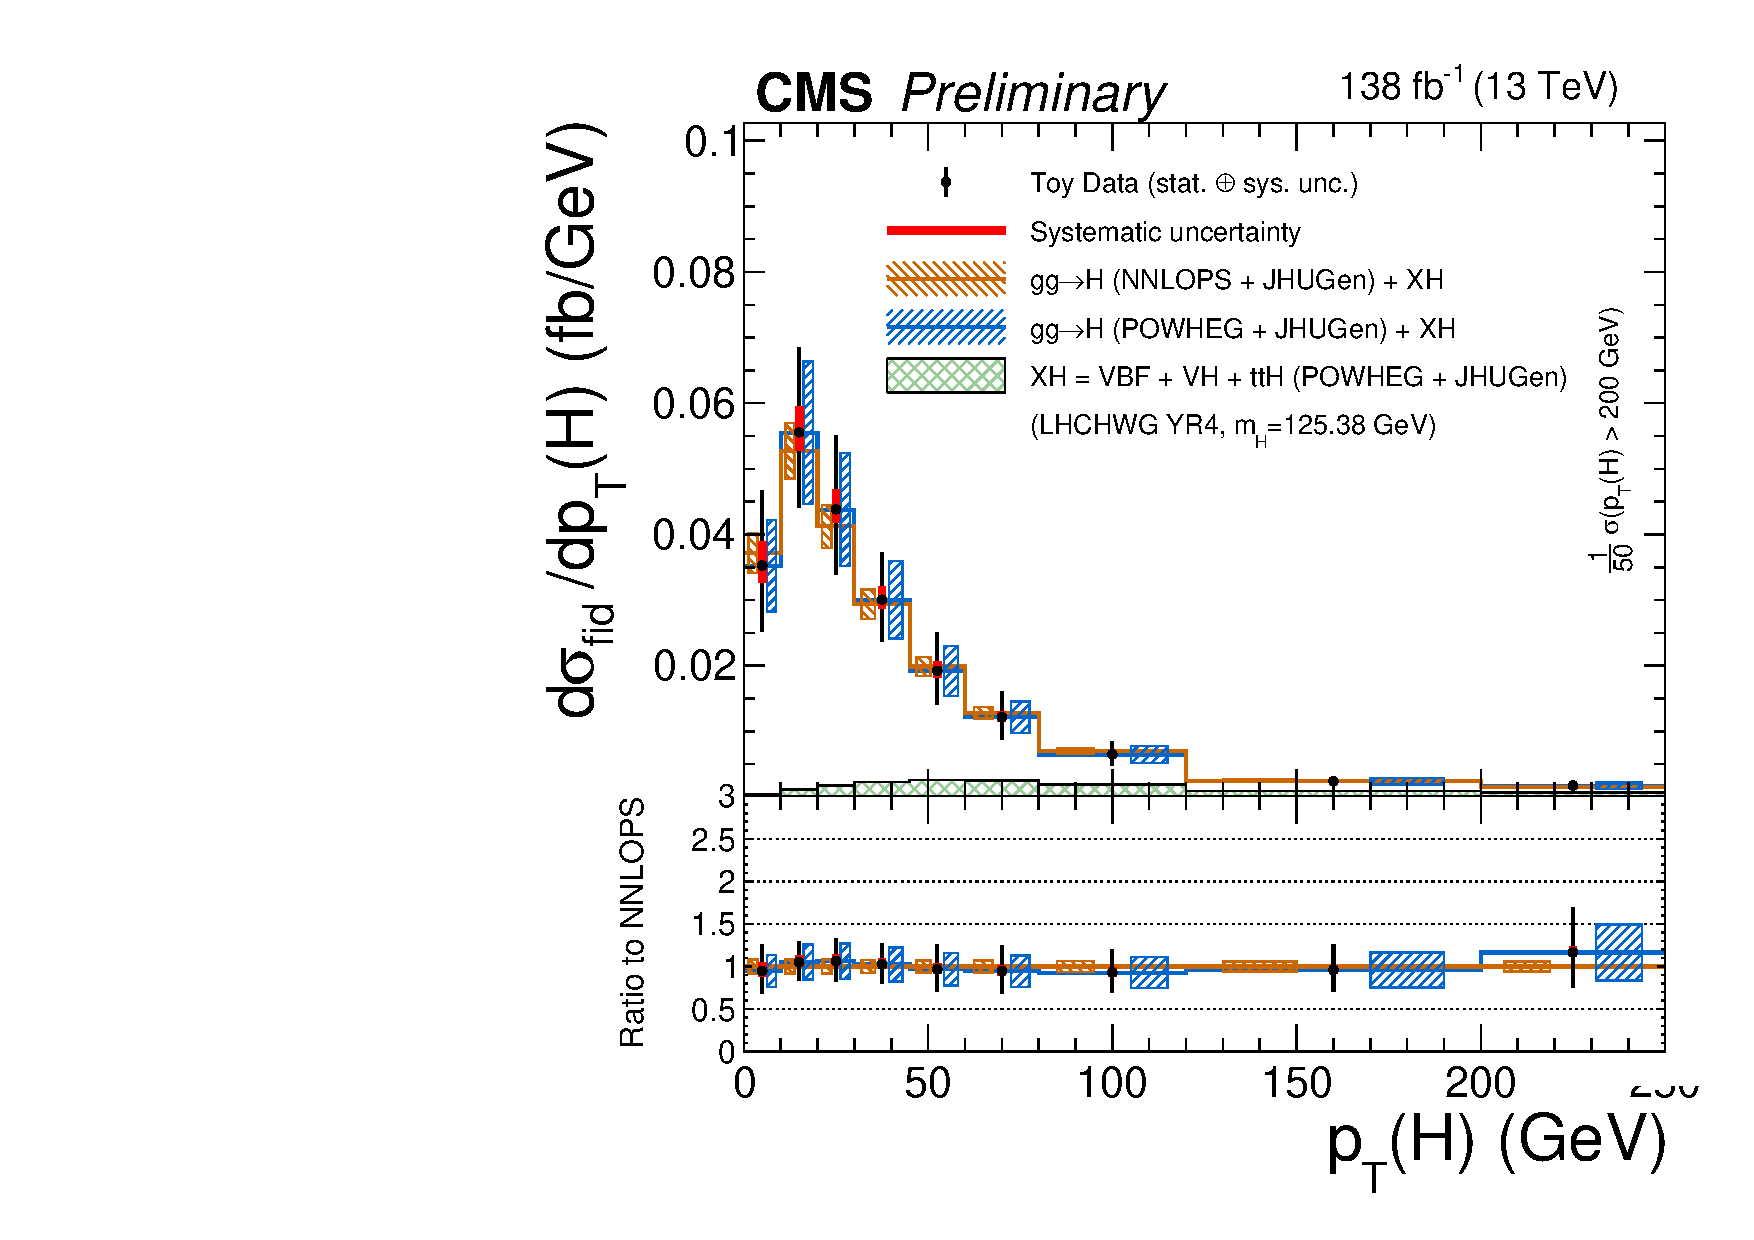
\includegraphics[width=0.48\textwidth]{Images/H4L/pT4l_unfoldwith_SM_125_asimov.pdf}
		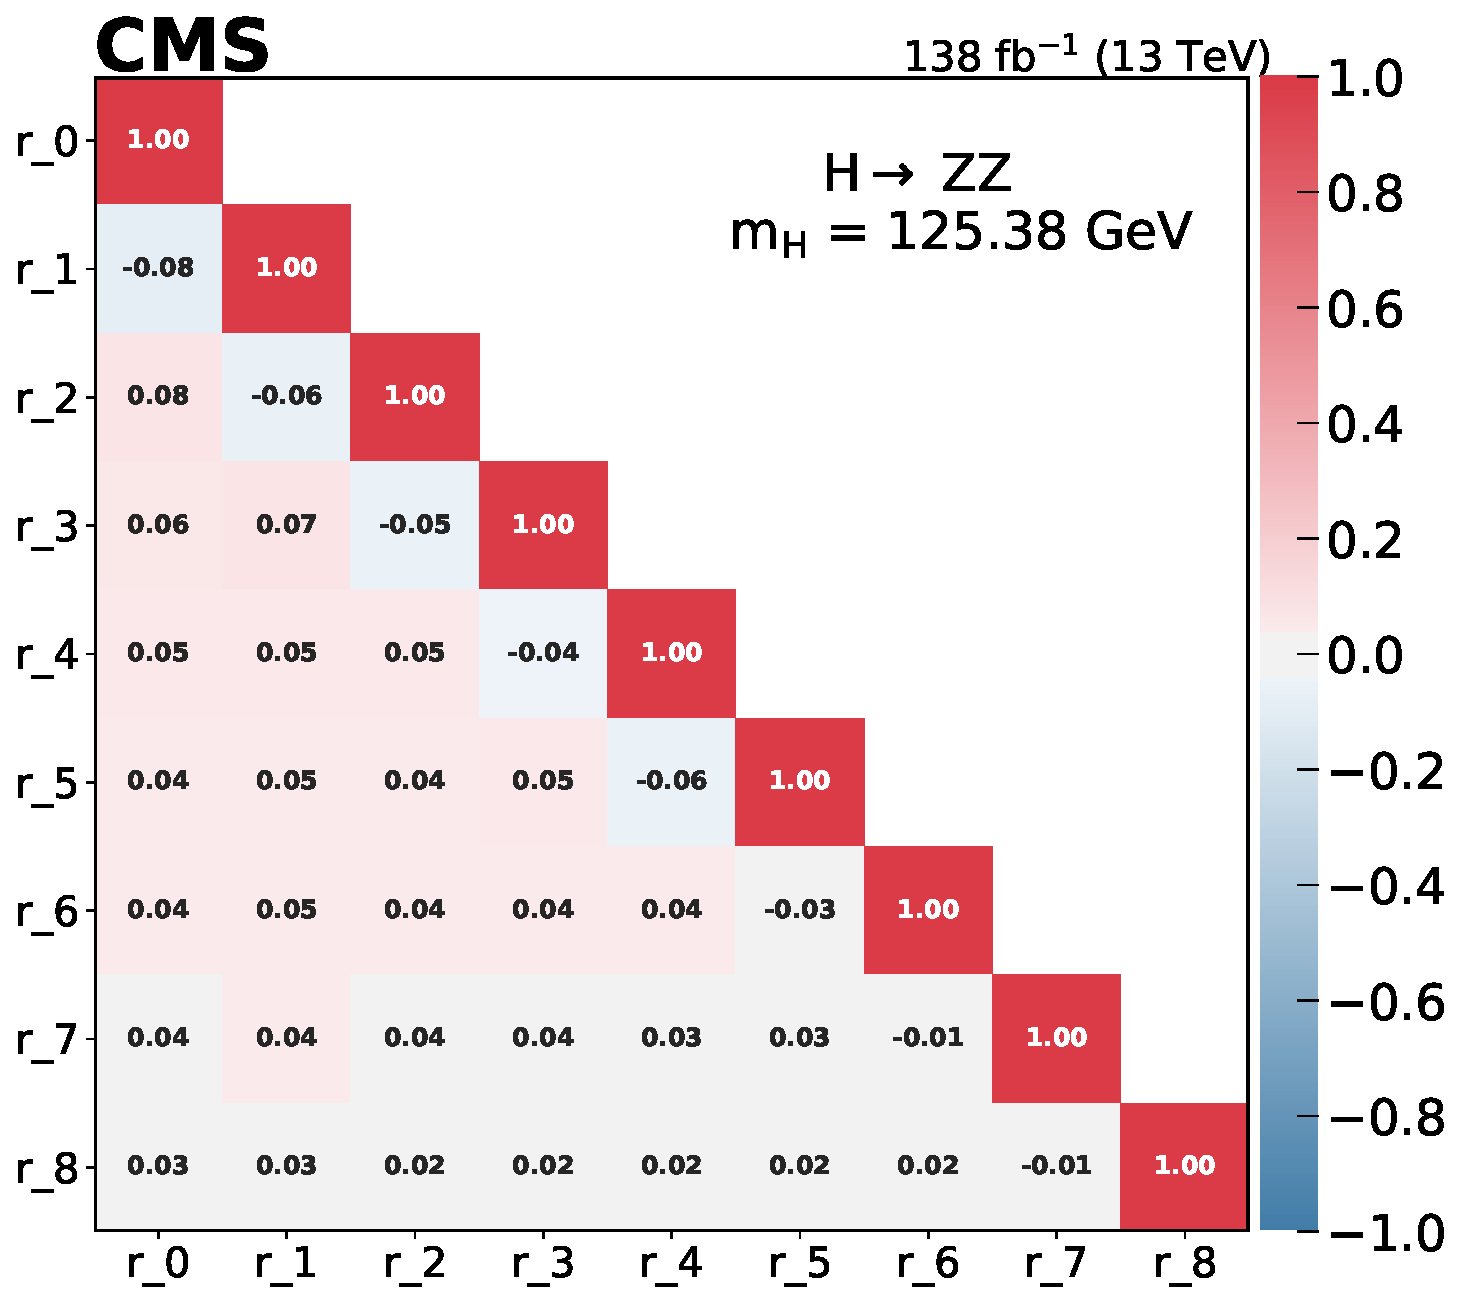
\includegraphics[width=0.48\textwidth]{Images/H4L/correlations/corr_pT4l_v3.pdf}\\
		\caption{
			Differential cross sections as a function of the transverse momentum of the Higgs boson $\pt^{\PH}$ (left) and the correlation matrix between the observed differential cross sections (right). 
			The acceptance and theoretical uncertainties in the differential bins are calculated using the $\ggH$ predictions from the \POWHEG generator (blue) normalised to $\mathrm{N^3LO}$.
			The sub-dominant component of the signal ($\VBF + \VH + \ttH$) is denoted as XH and are fixed to the SM.
			The measured cross sections are also compared with the ggH predictions from the NNLOPS (orange) and MadGraph\_aMC@NLO (pink) generators.
			The black points represent the measured fiducial cross sections in each bin, while the black error bars represent the total uncertainty on each measurement.
			The red boxes depict the systematic components of the uncertainties introduced in Sec.~\ref{sec:systematics}.
			\label{fig:fidPTH}}
	\end{figure}
\end{center}

\clearpage

\begin{center}
	\begin{figure}[!htbp]
		\centering
		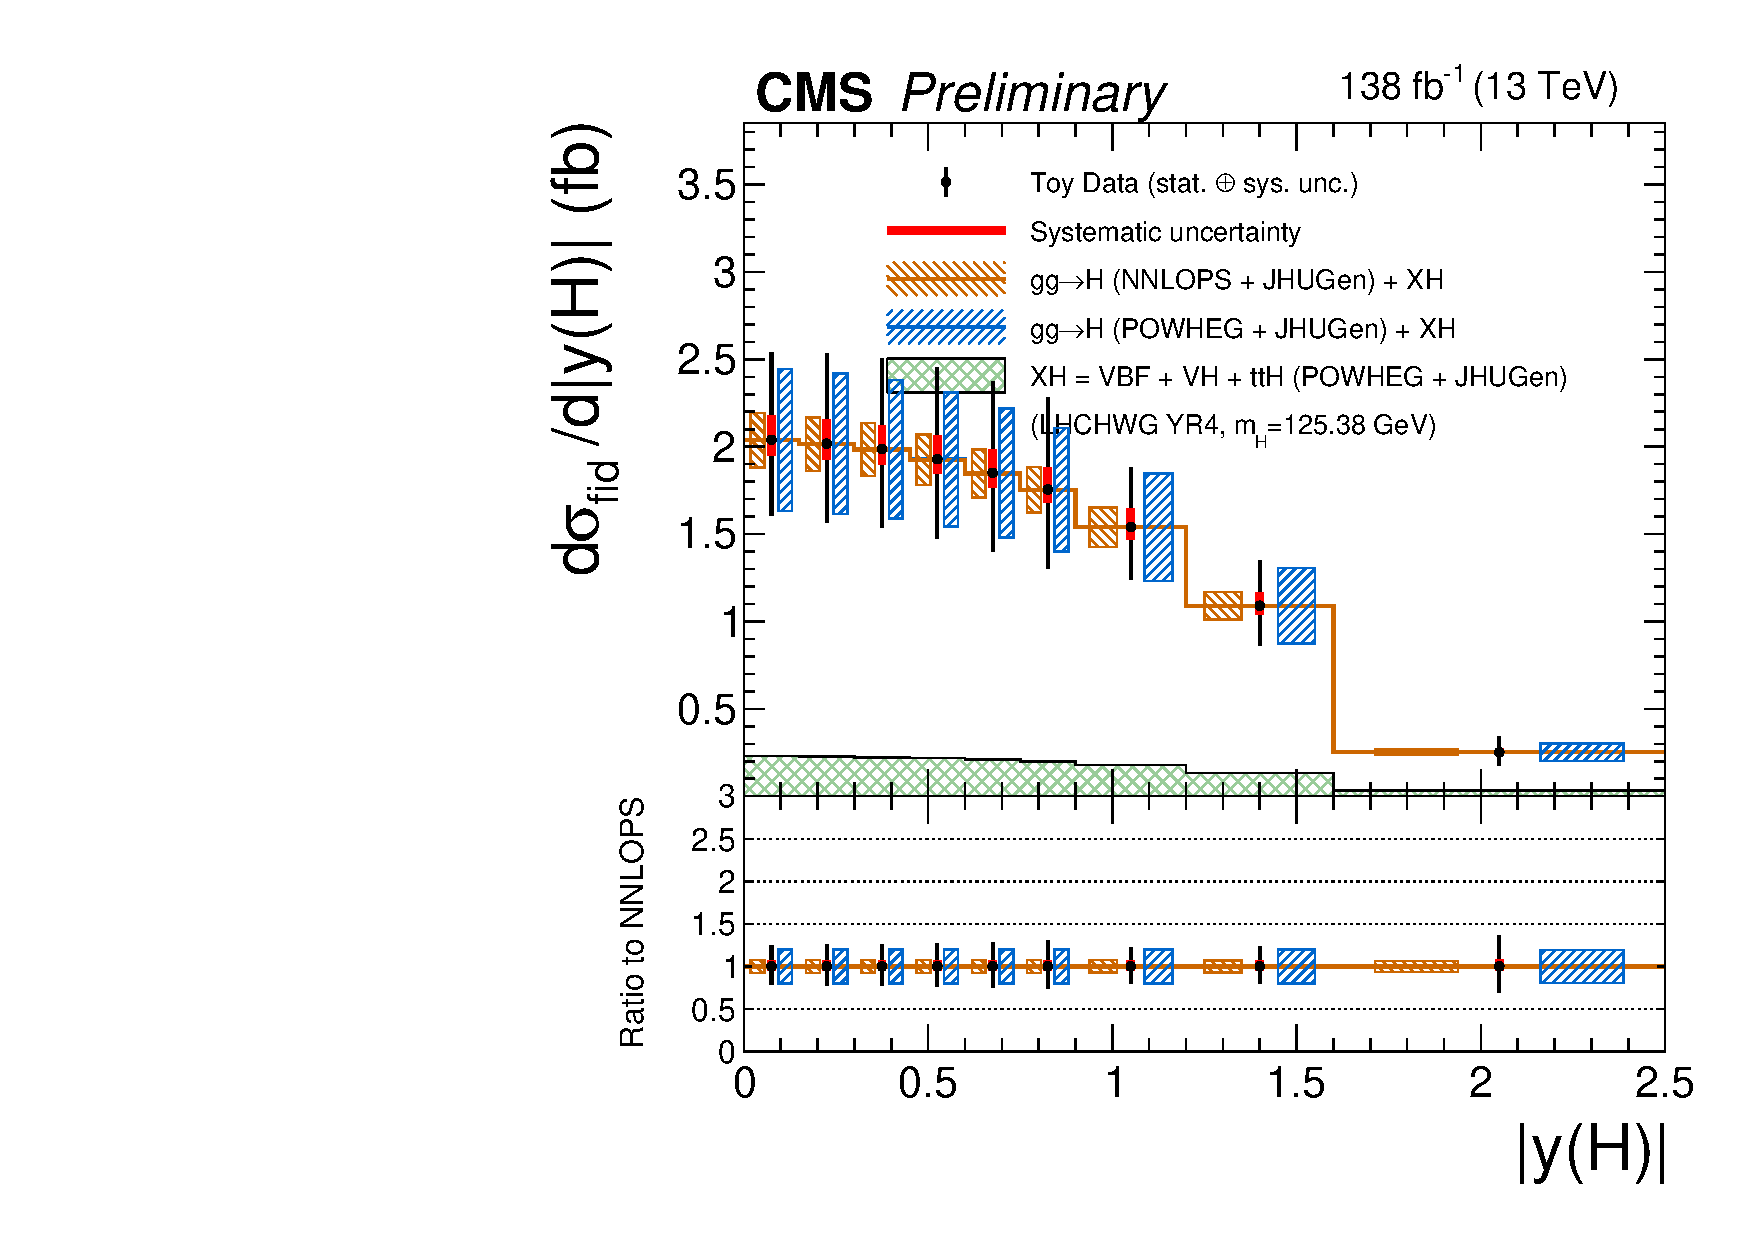
\includegraphics[width=0.48\textwidth]{Images/H4L/rapidity4l_unfoldwith_SM_125_asimov.pdf}
		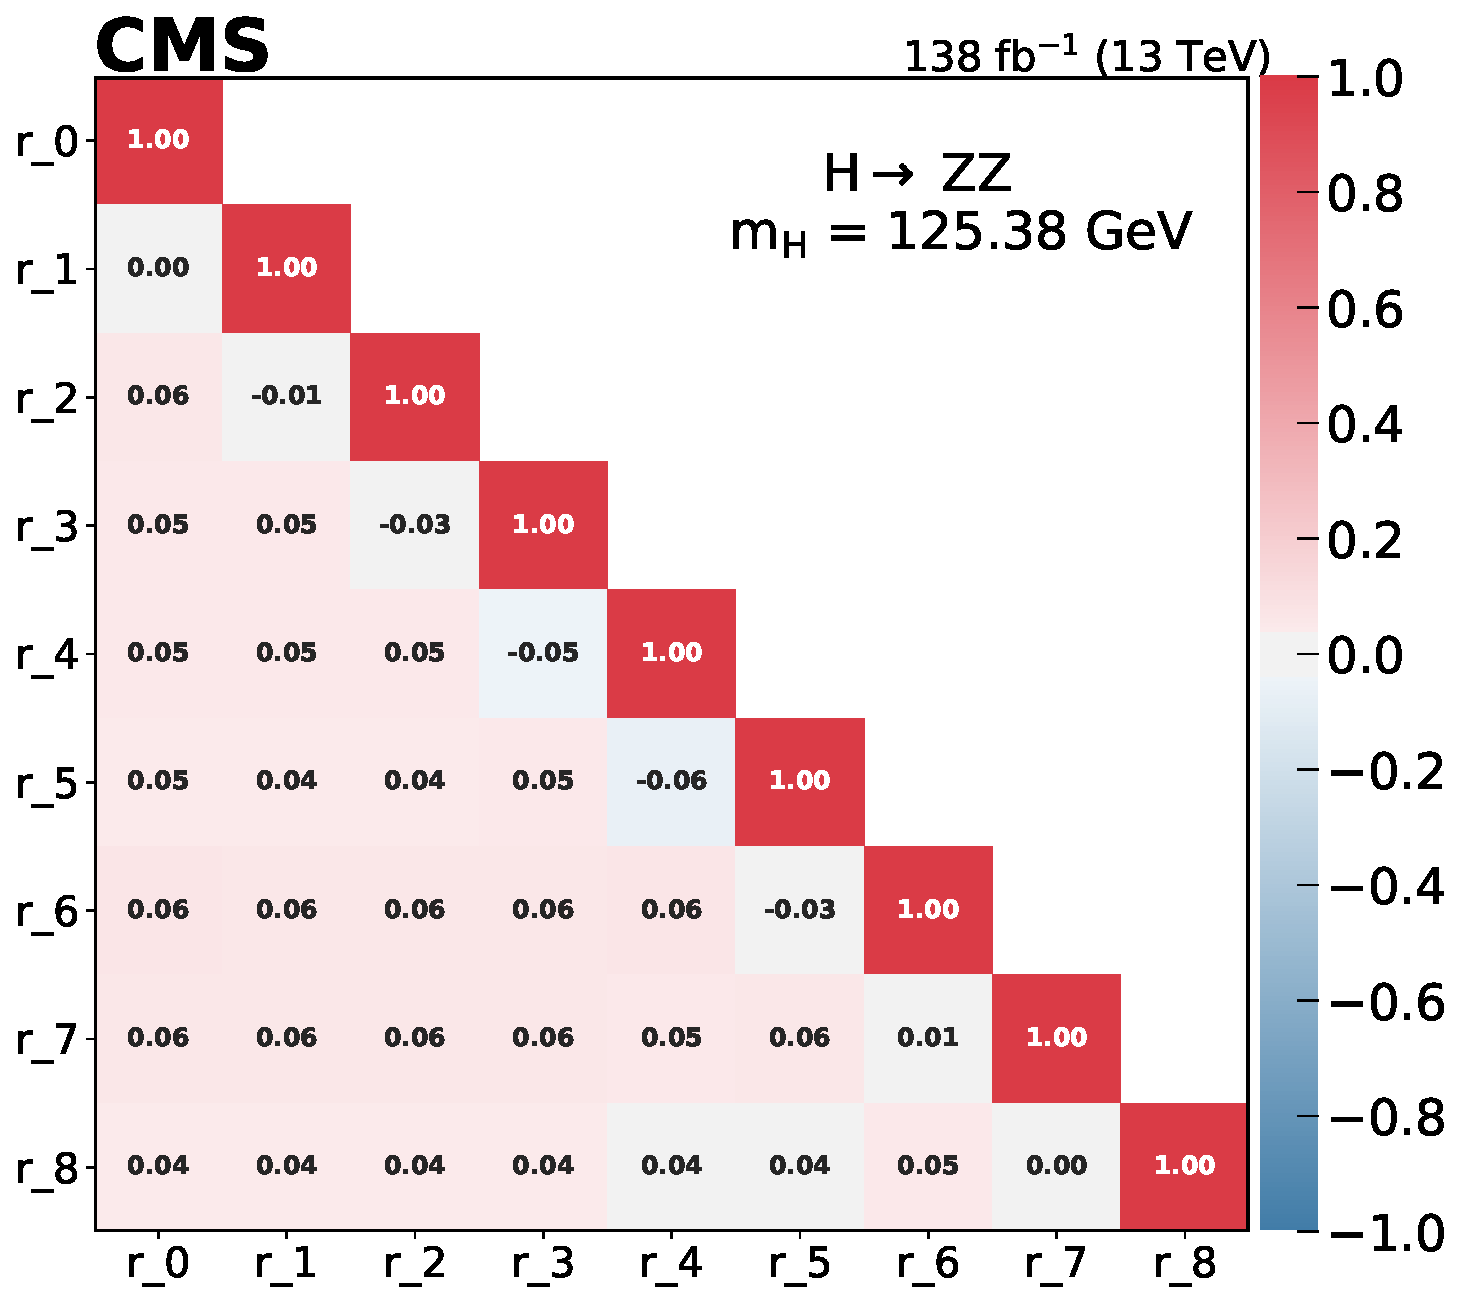
\includegraphics[width=0.48\textwidth]{Images/H4L/correlations/corr_rapidity4l_v3.pdf}\\
		\caption{
			Differential cross sections as a function of  the rapidity of the Higgs boson $\abs{y^{\PH}}$ (left) and the correlation matrix between the observed differential cross sections (right).
			The acceptance and theoretical uncertainties in the differential bins are calculated using the \POWHEG (blue), NNLOPS (orange), and MadGraph\_aMC@NLO (pink) generators.
			The sub-dominant component of the signal ($\VBF + \VH + \ttH$) is denoted as XH and it is fixed to the SM.
			\label{fig:fidYH}}
	\end{figure}
\end{center}

\clearpage

\begin{center}
	\begin{figure}[!htb]
		\centering
		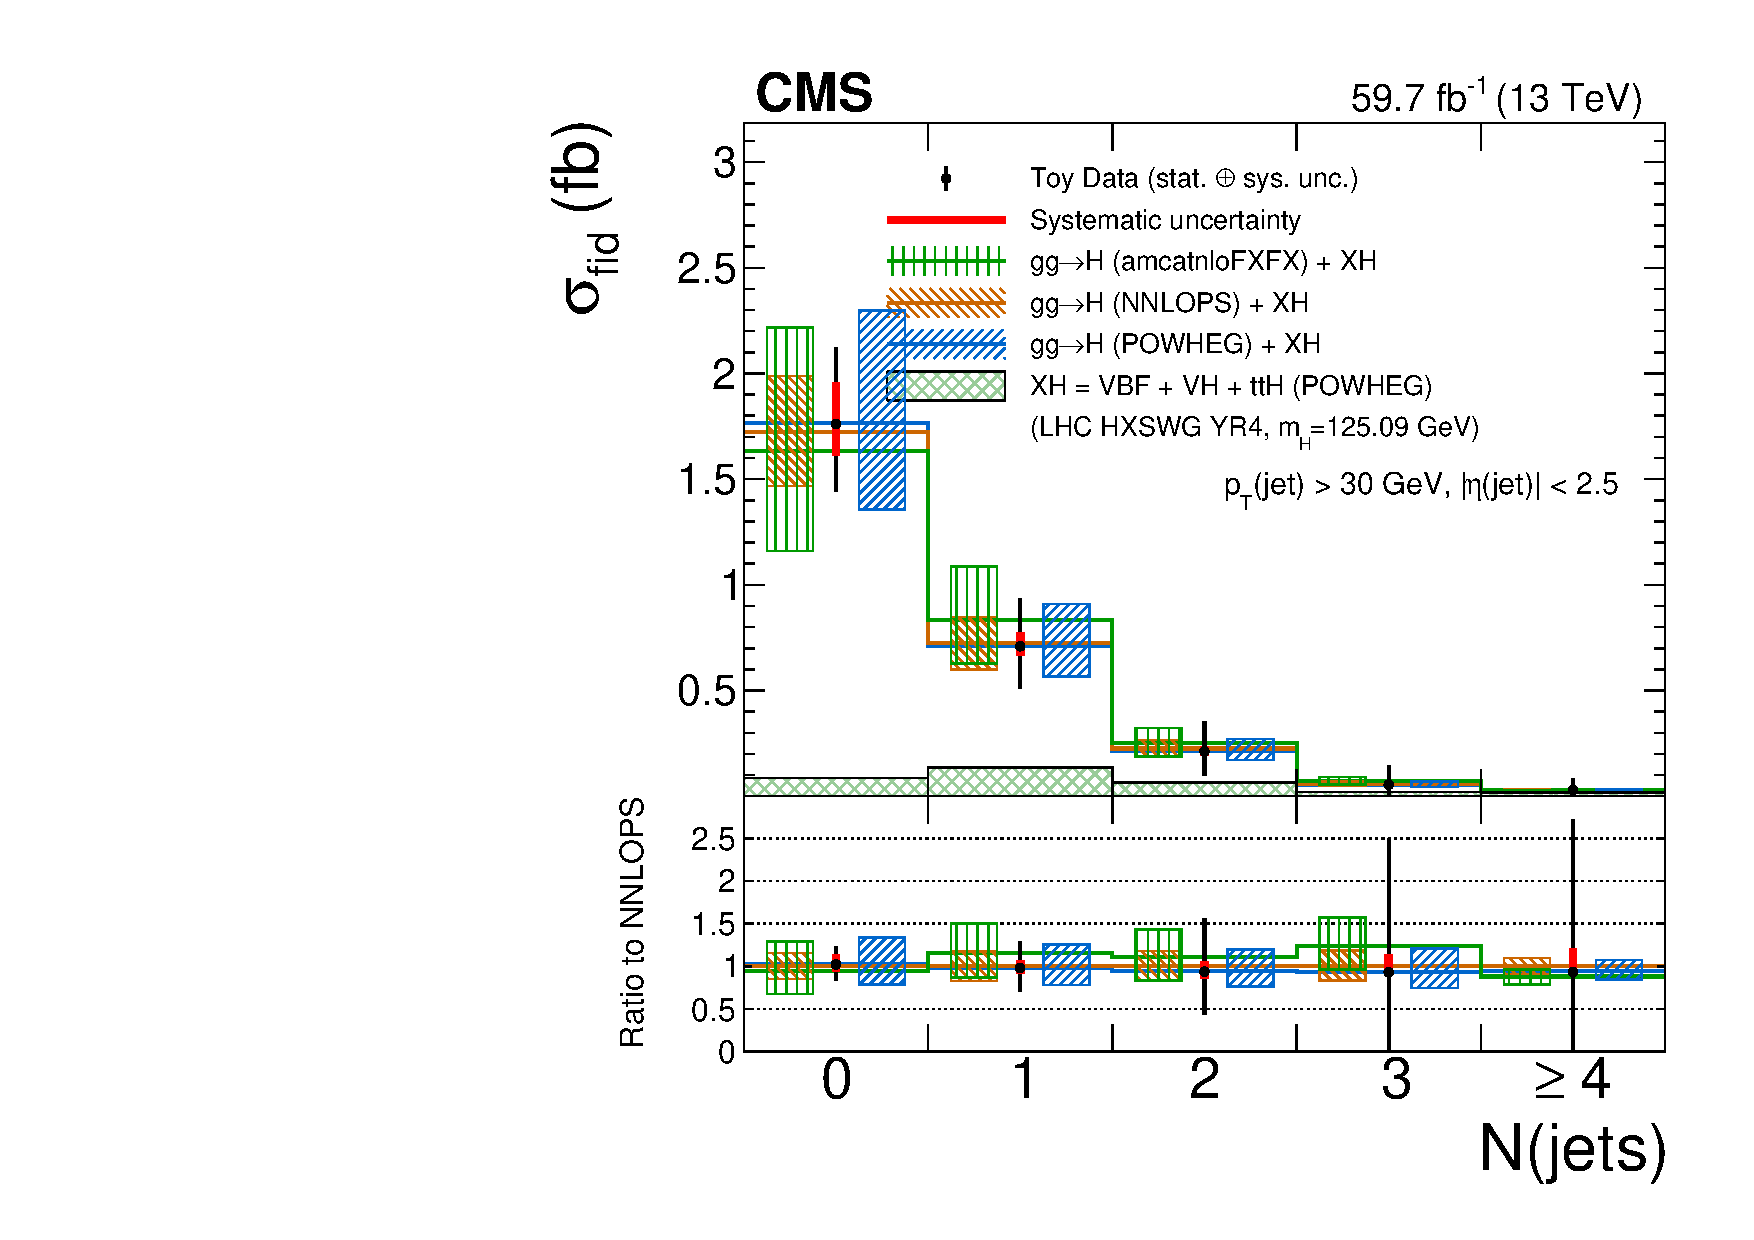
\includegraphics[width=0.48\textwidth]{Images/H4L/njets_pt30_eta2p5_unfoldwith_SM_125_asimov.pdf}
		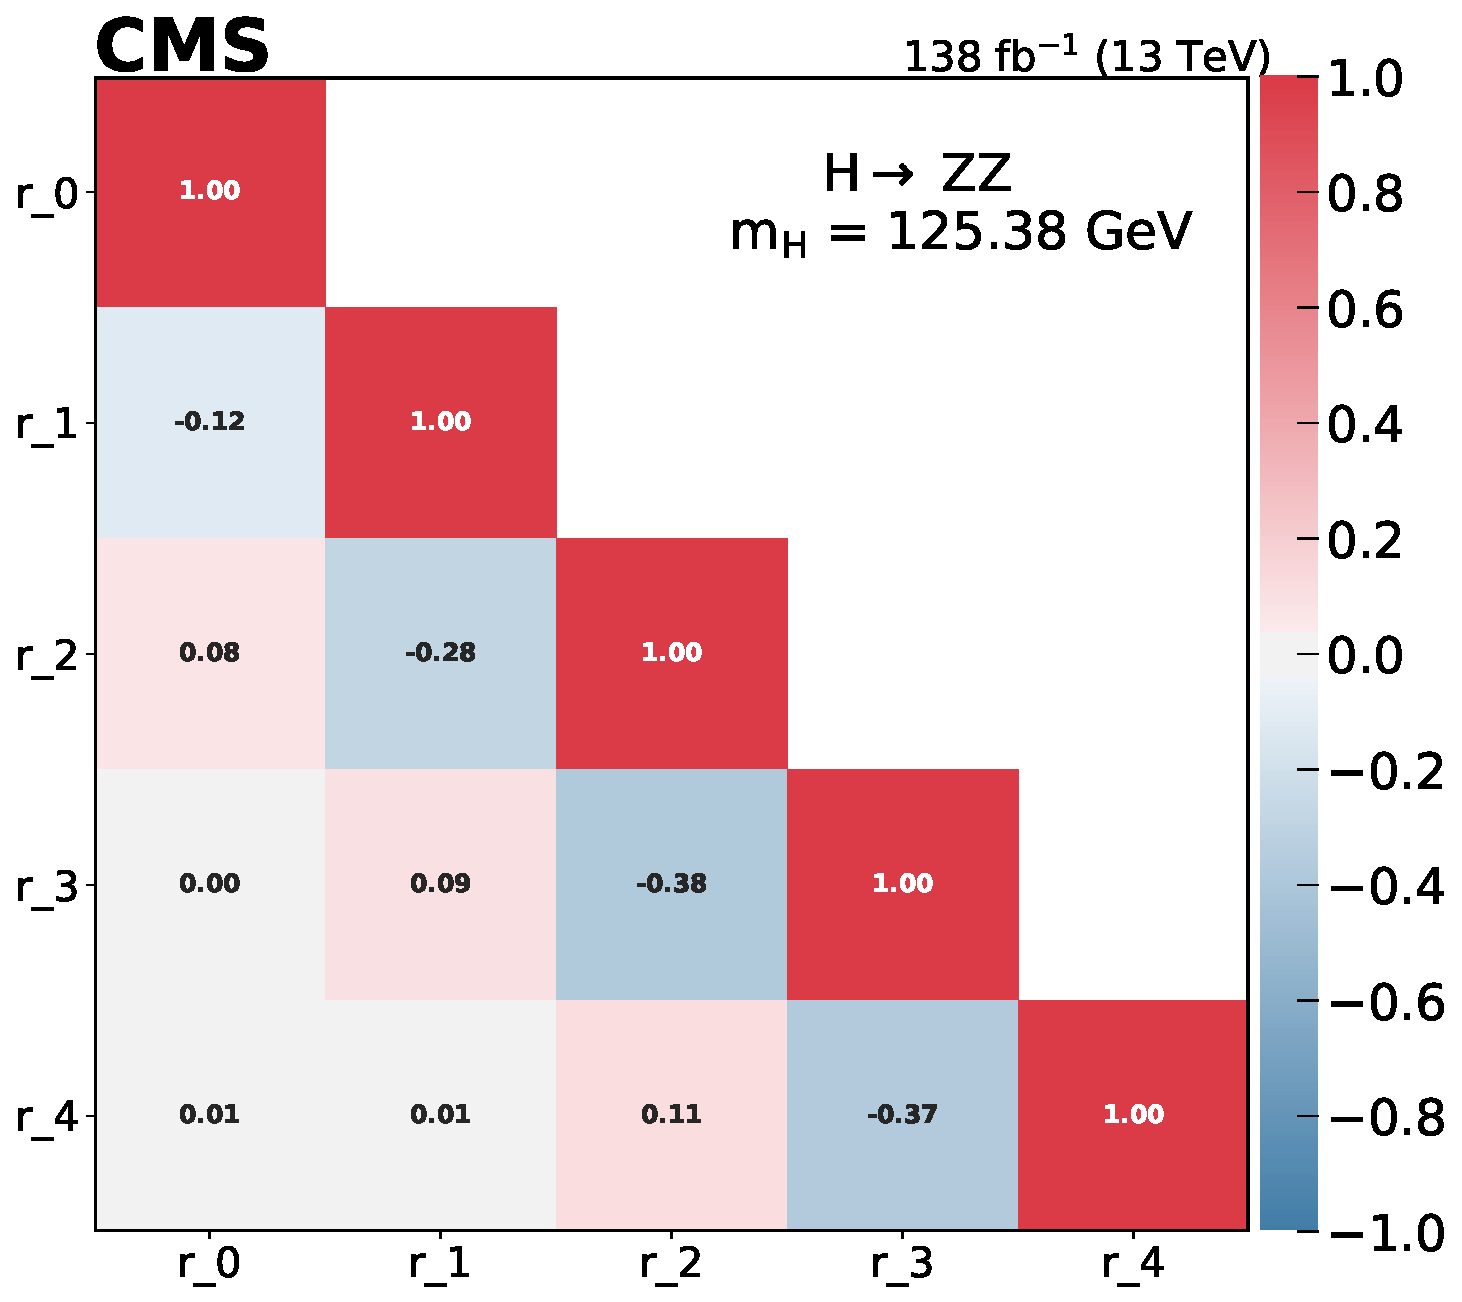
\includegraphics[width=0.48\textwidth]{Images/H4L/correlations/corr_njets_pt30_eta4p7_v3.pdf}\\
		\caption{
			Differential cross sections as a function of the number of associated jets in the event (left) and the correlation matrix between the observed differential cross sections (right).
			The acceptance and theoretical uncertainties in the differential bins are calculated using the \POWHEG (blue), NNLOPS (orange), and MadGraph\_aMC@NLO (pink) generators.
			The sub-dominant component of the signal ($\VBF + \VH + \ttH$) is denoted as XH and it is fixed to the SM.
			\label{fig:fidNJ}}
	\end{figure}
\end{center}

\clearpage

\begin{center}
	\begin{figure}[!htb]
		\centering
		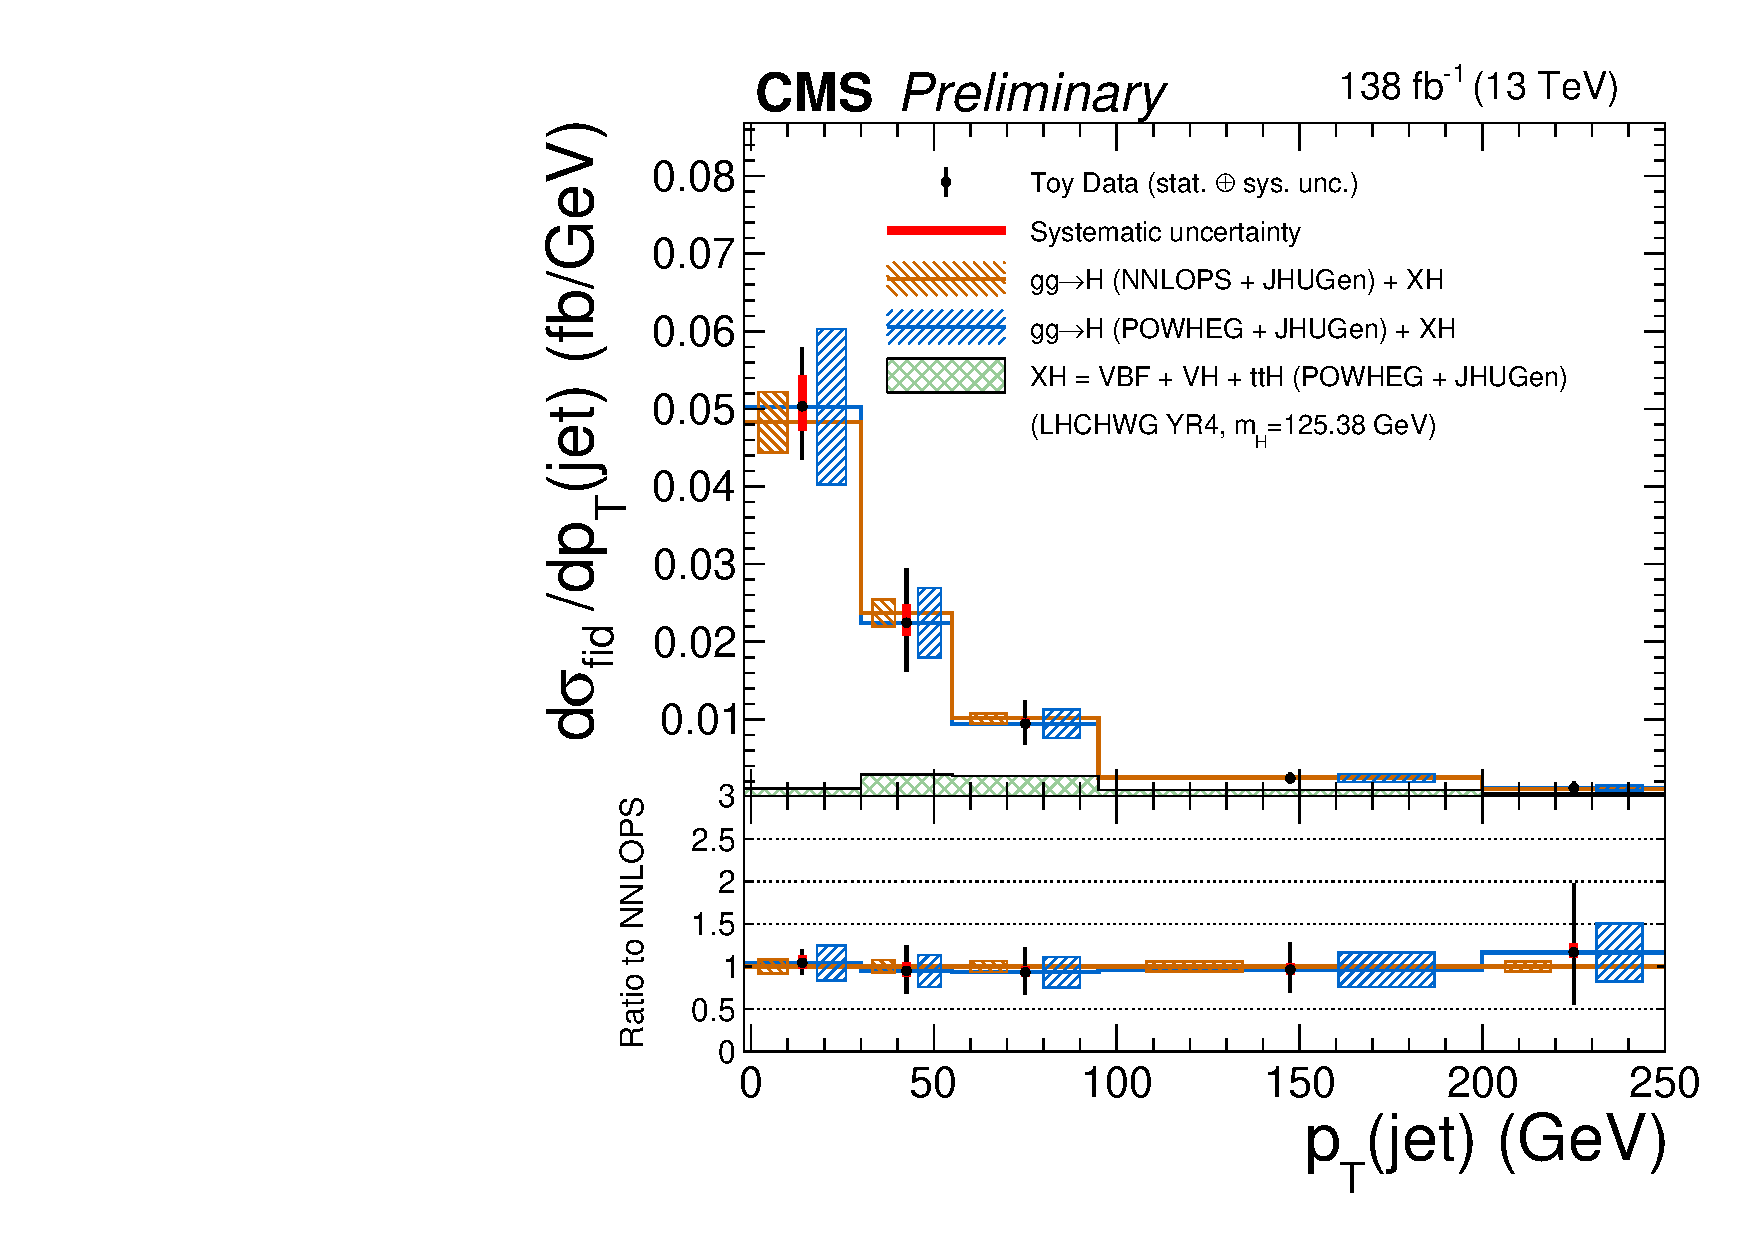
\includegraphics[width=0.48\textwidth]{Images/H4L/pTj1_unfoldwith_SM_125_asimov.pdf}
		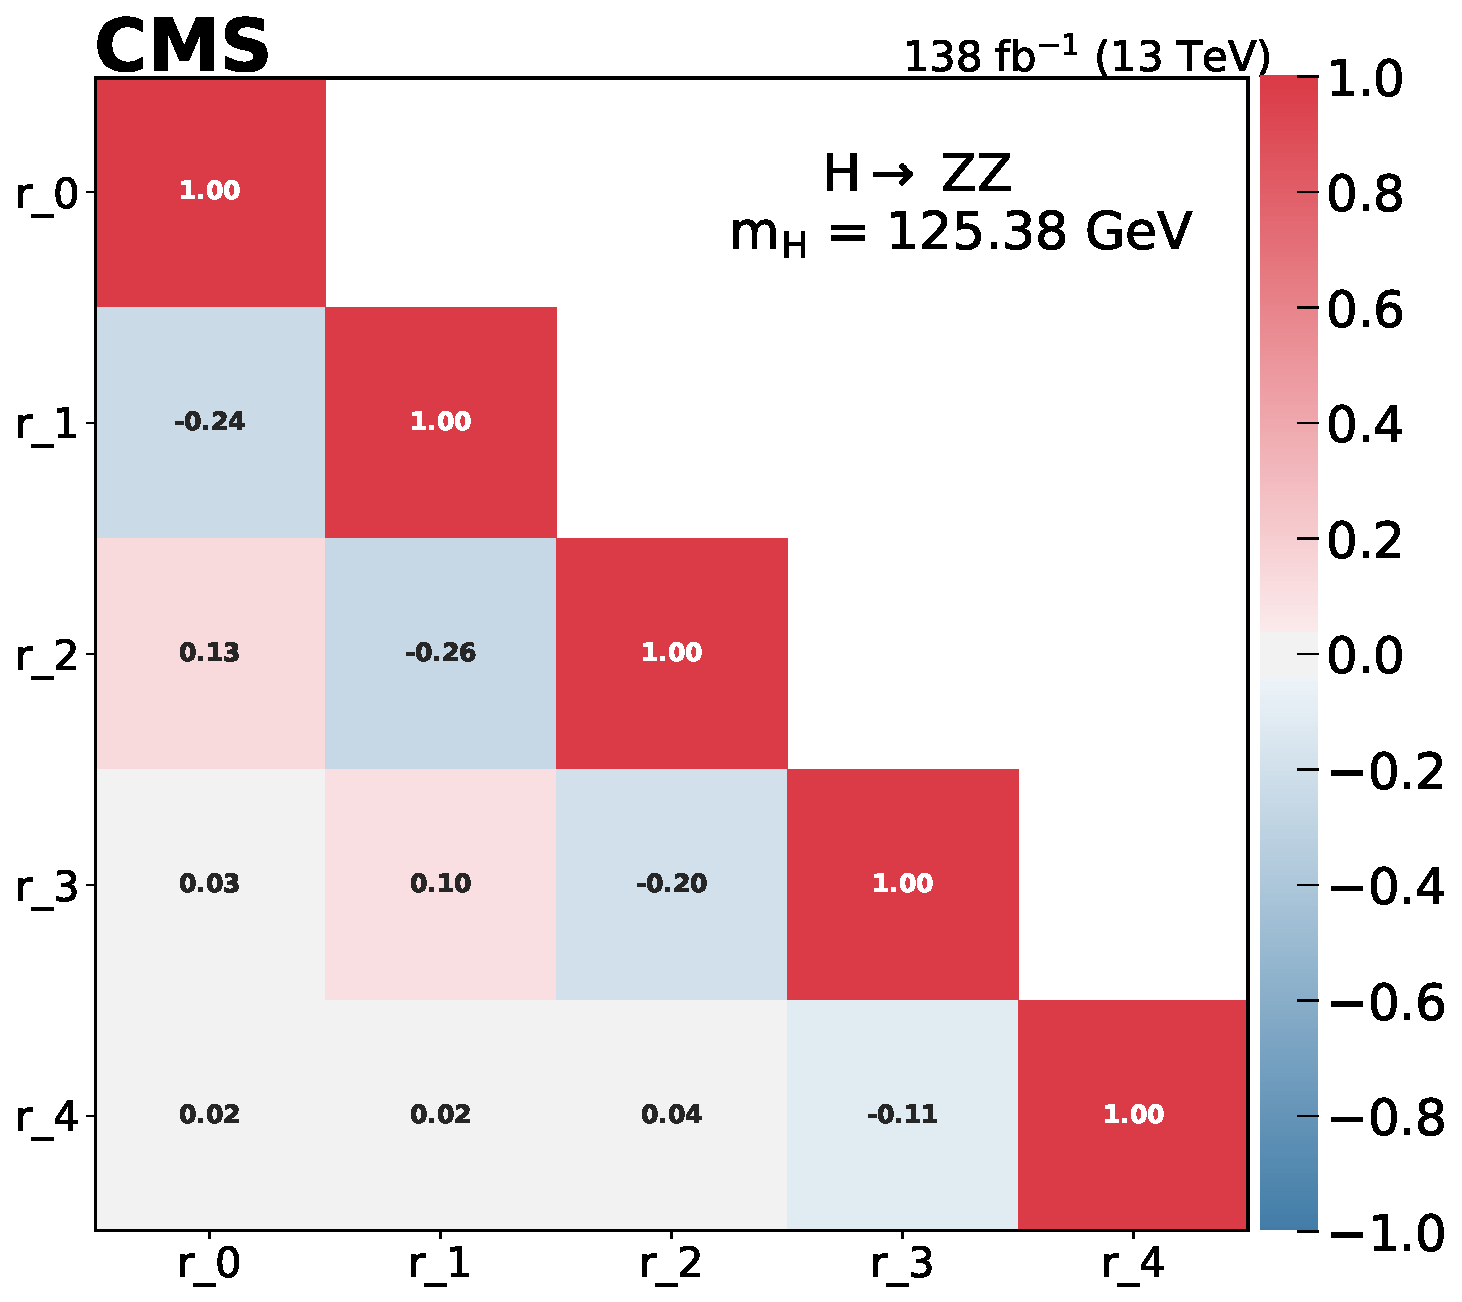
\includegraphics[width=0.48\textwidth]{Images/H4L/correlations/corr_pTj1_v3.pdf}\\
		\caption{
			Differential cross sections as a function of the \pt of the leading jet in the event (left) and the correlation matrix between the observed differential cross sections (right).
			The acceptance and theoretical uncertainties in the differential bins are calculated using the \POWHEG (blue), NNLOPS (orange), and MadGraph\_aMC@NLO (pink) generators.
			The sub-dominant component of the signal ($\VBF + \VH + \ttH$) is denoted as XH and it is fixed to the SM.
			\label{fig:fidPTJ1}}
	\end{figure}
\end{center}

\clearpage

\begin{center}
	\begin{figure}[!htb]
		\centering
		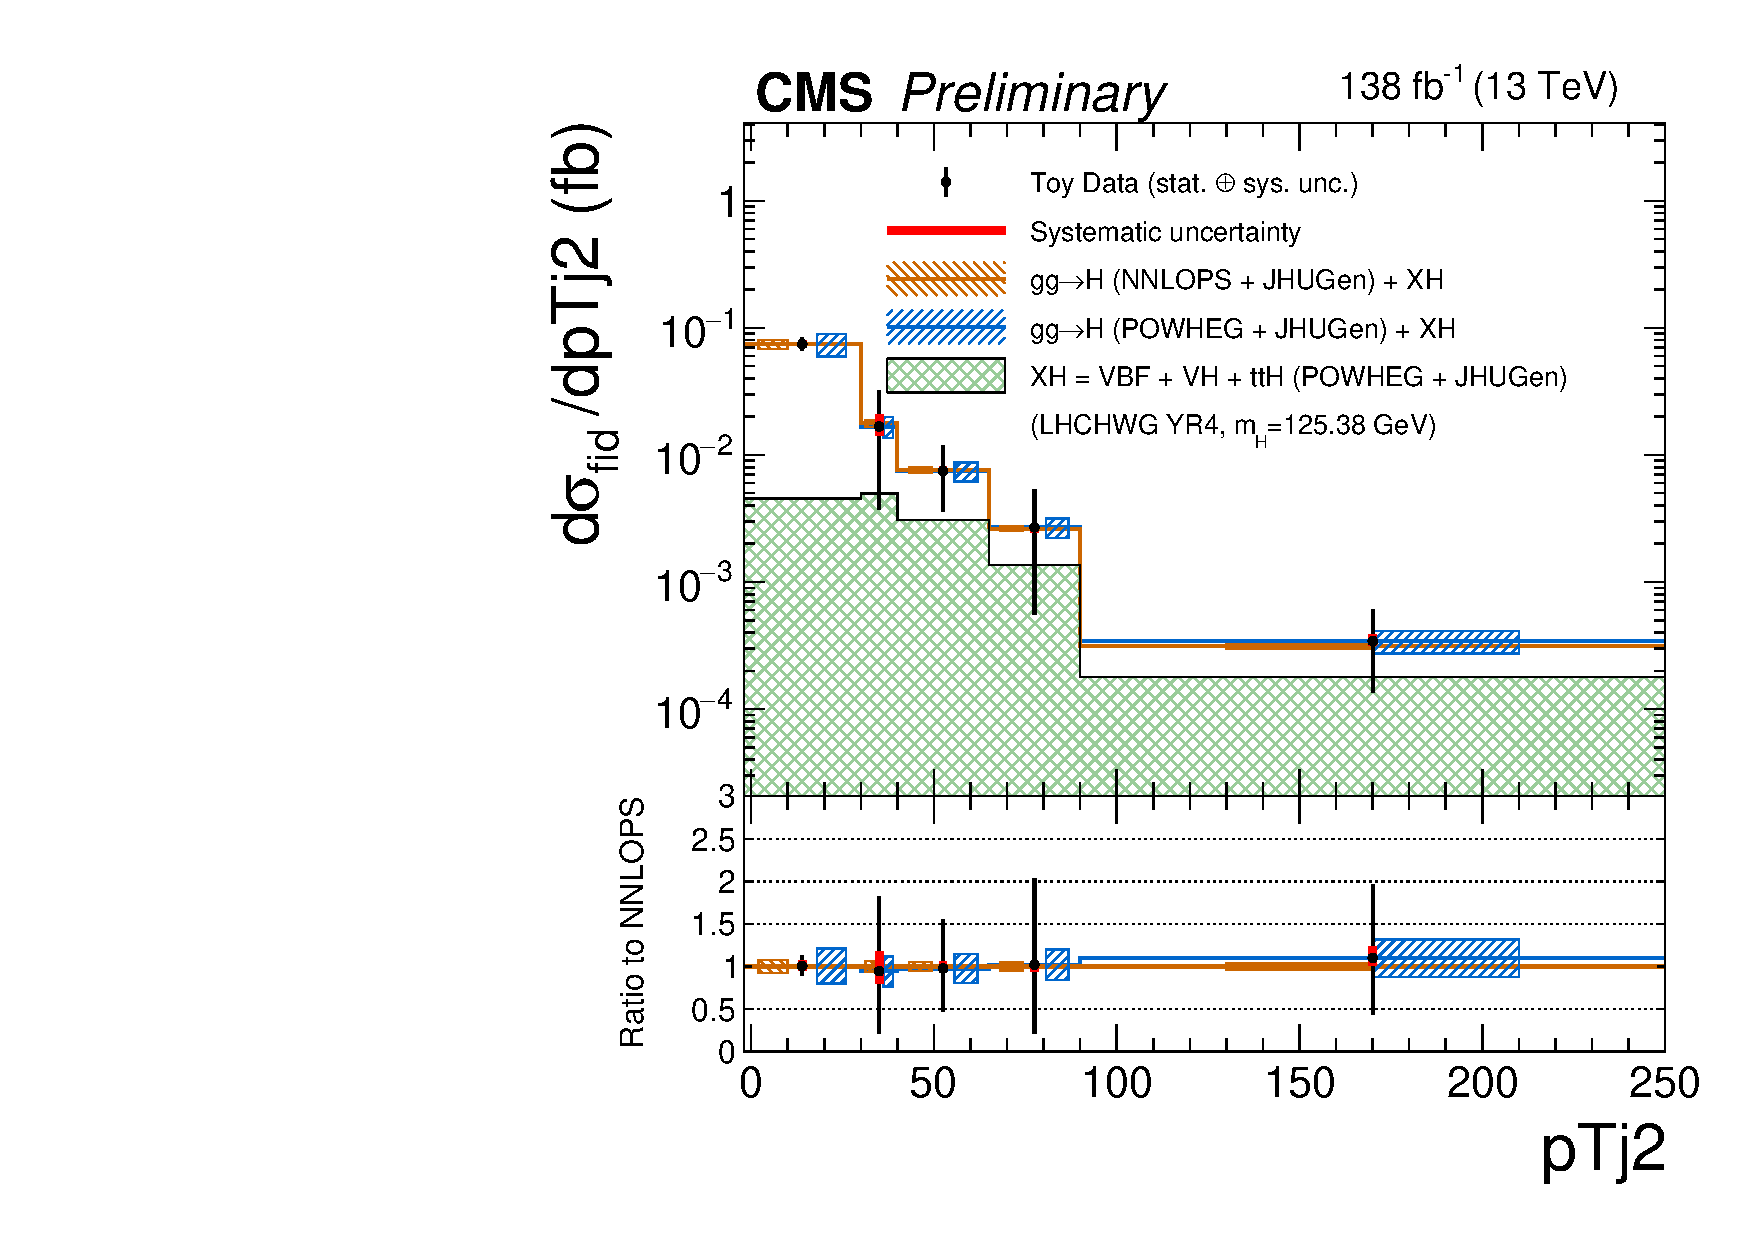
\includegraphics[width=0.48\textwidth]{Images/H4L/pTj2_unfoldwith_SM_125_logscale_asimov.pdf}	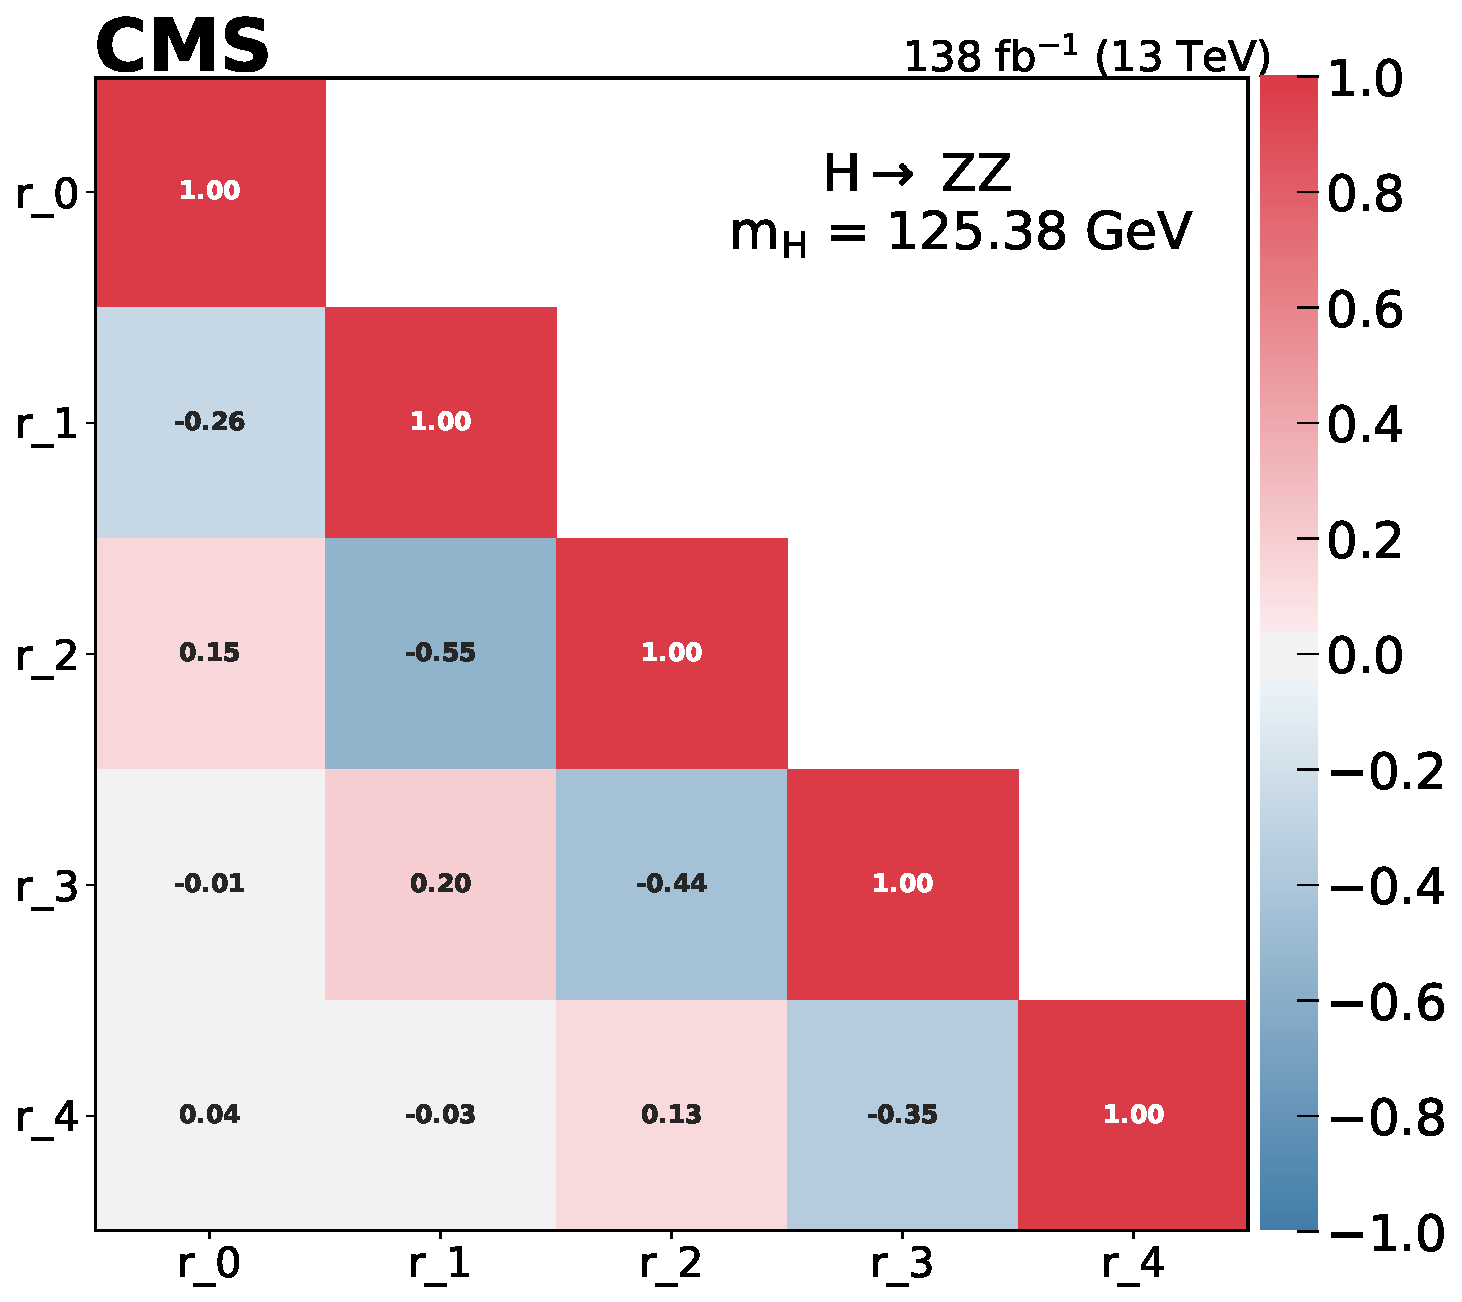
\includegraphics[width=0.48\textwidth]{Images/H4L/correlations/corr_pTj2_v3.pdf}\\
		\caption{
			Differential cross sections as a function of the \pt of the sub-leading jet in the event (left) and the correlation matrix between the observed differential cross sections (right).
			The acceptance and theoretical uncertainties in the differential bins are calculated using the \POWHEG (blue), NNLOPS (orange), and MadGraph\_aMC@NLO (pink) generators.
			The sub-dominant component of the signal ($\VBF + \VH + \ttH$) is denoted as XH and it is fixed to the SM.
			\label{fig:fidPTJ2}}
	\end{figure}
\end{center}

\clearpage

%%%%%%%%%%%%%%%%%%%%%%%% Dijet system %%%%%%%%%%%%%%%%%%%%%%%%%

\begin{center}
	\begin{figure}[!htb]
		\centering
		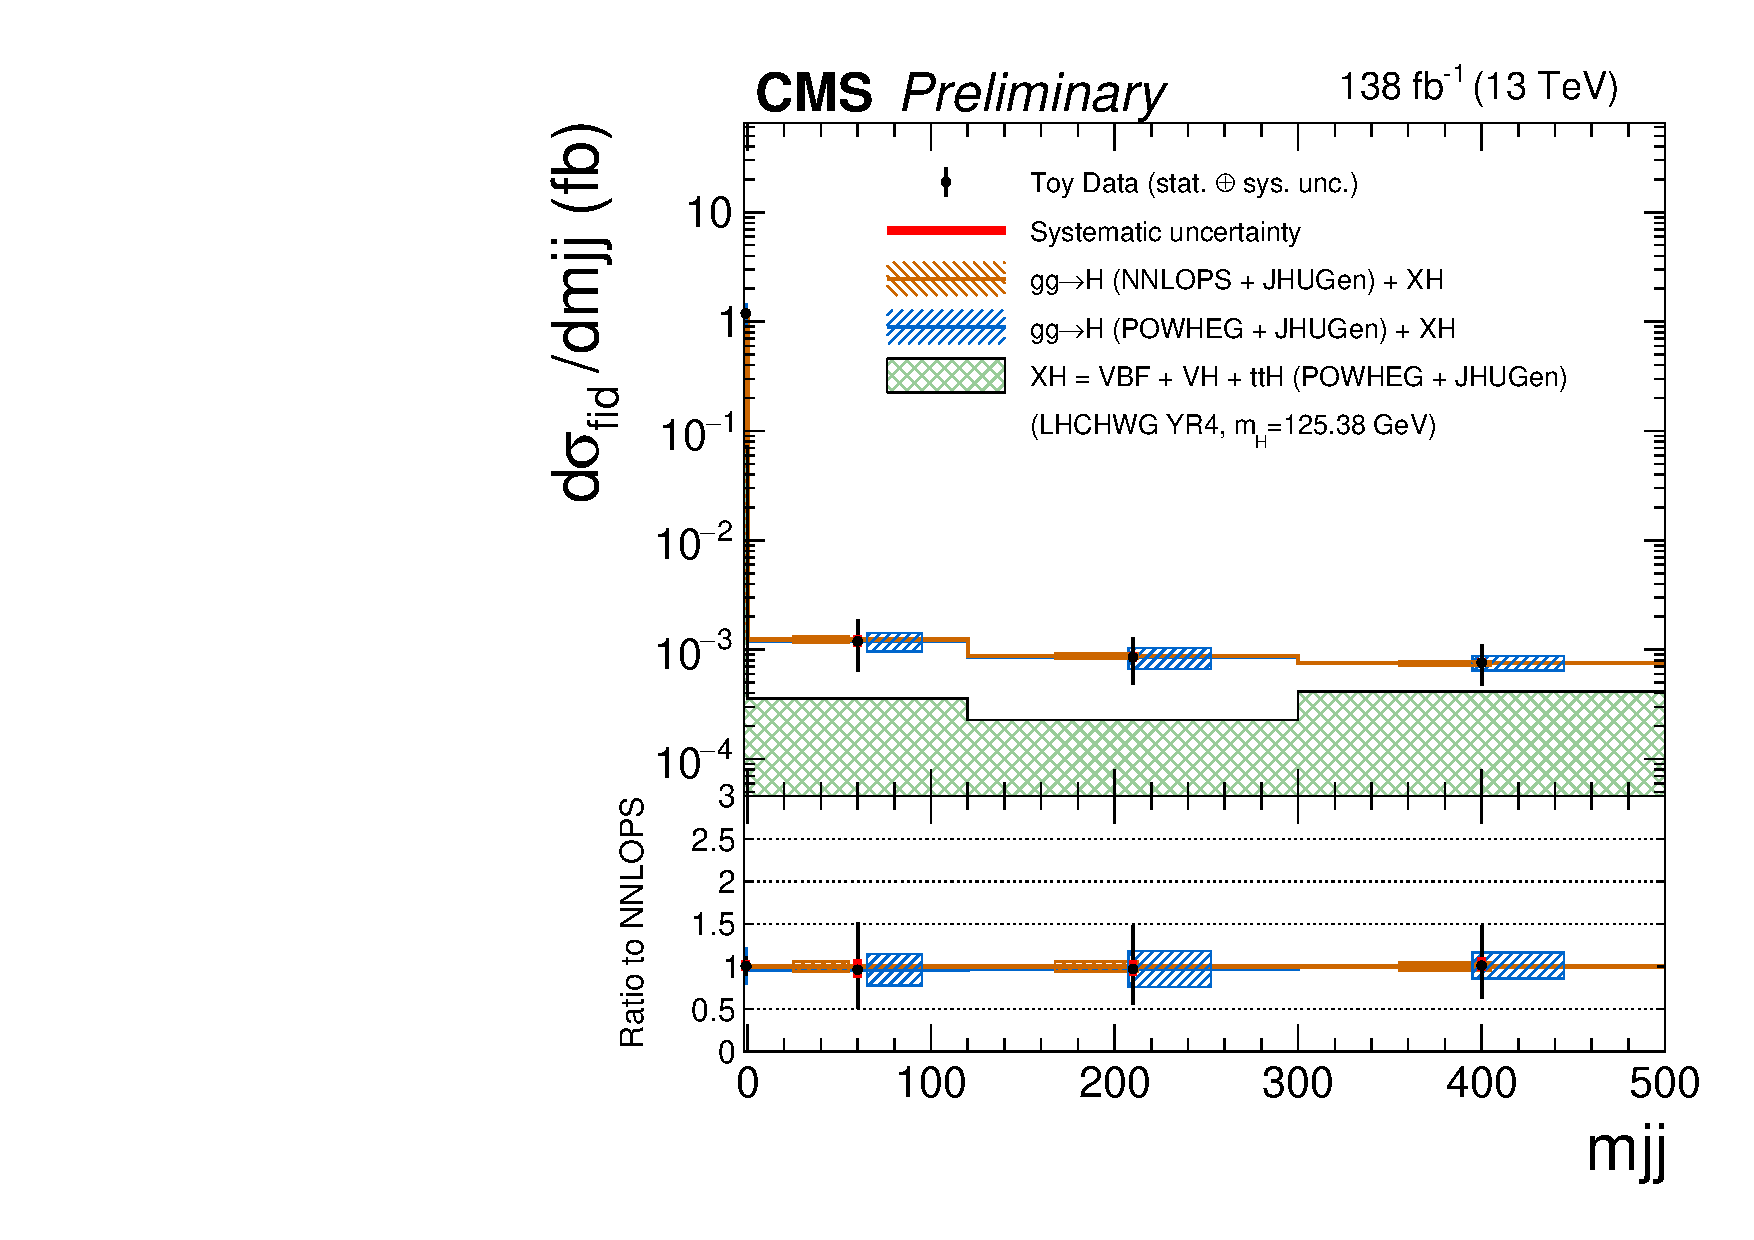
\includegraphics[width=0.48\textwidth]{Images/H4L/mjj_unfoldwith_SM_125_logscale_asimov.pdf}	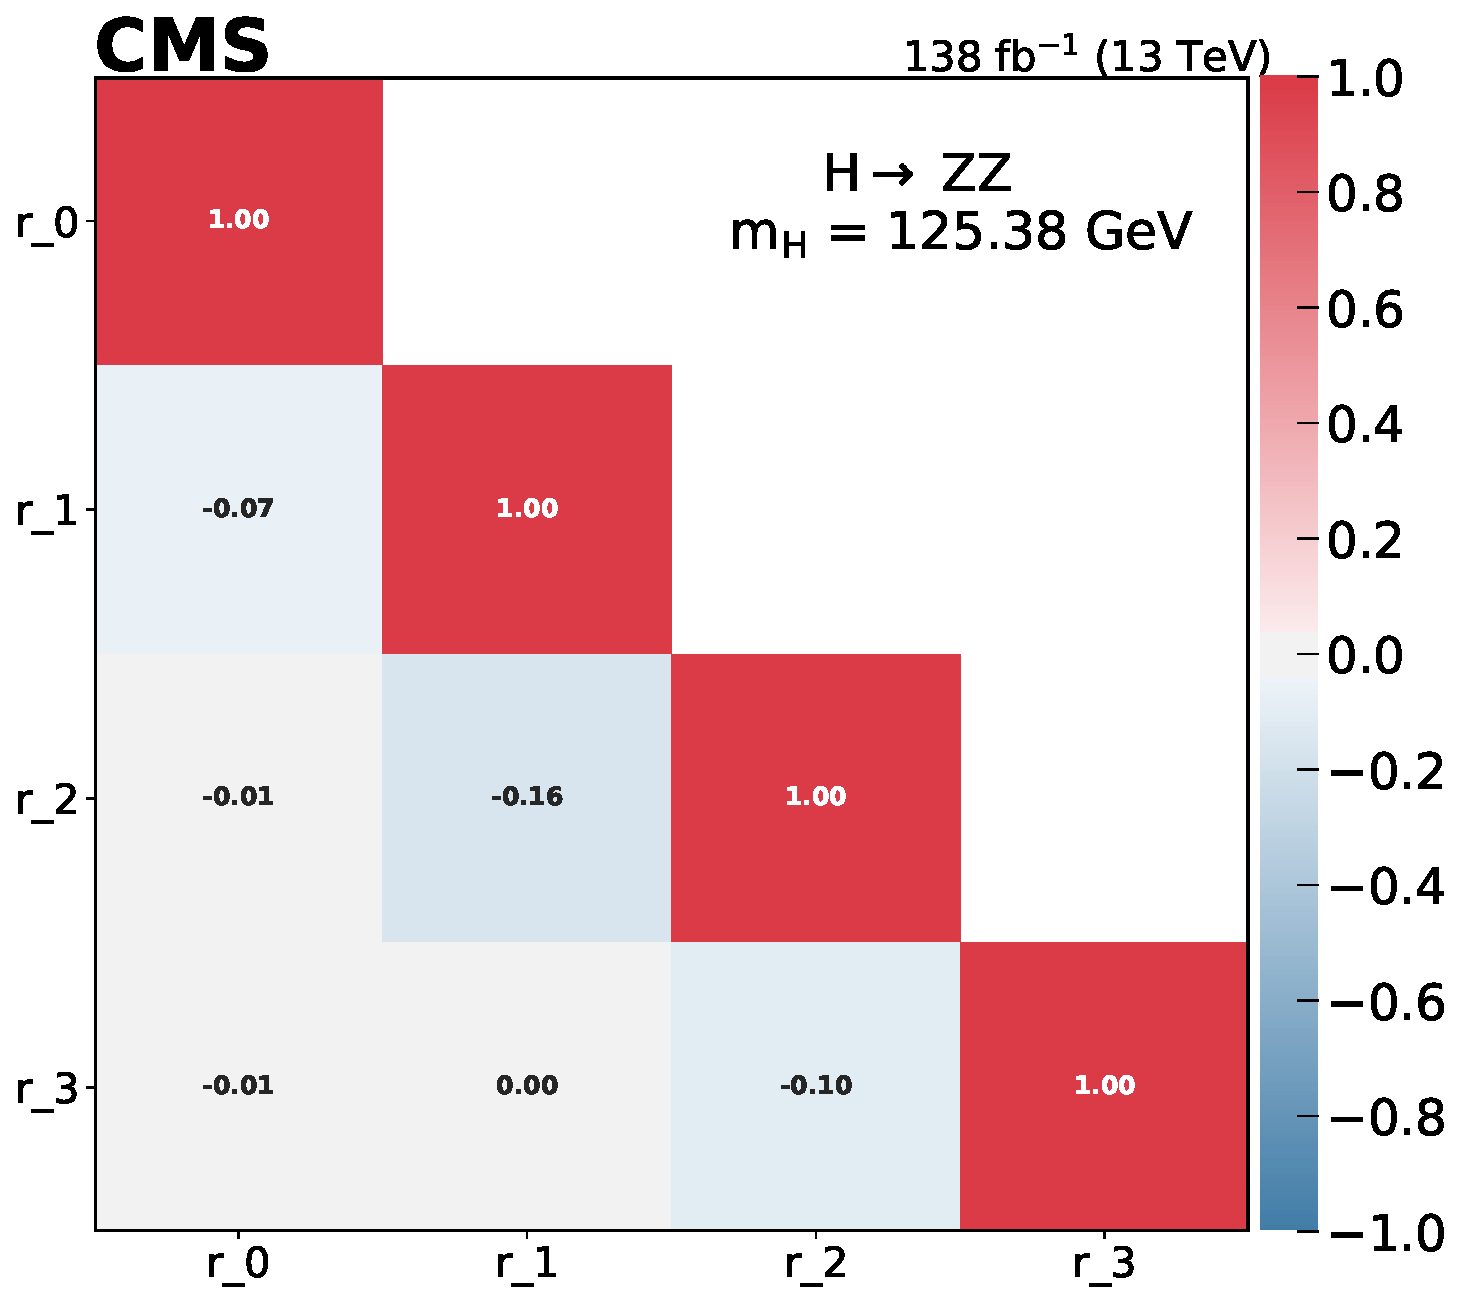
\includegraphics[width=0.48\textwidth]{Images/H4L/correlations/corr_mjj_v3.pdf}\\
		\caption{
			Differential cross sections as a function of the invariant mass of the di-jet system $m_{jj}$ (left) and the correlation matrix between the observed differential cross sections (right).
			The first bin comprises all those events with less than two jets, for which $m_{jj}$  is undefined.
			The acceptance and theoretical uncertainties in the differential bins are calculated using the \POWHEG (blue), NNLOPS (orange), and MadGraph\_aMC@NLO (pink) generators.
			The sub-dominant component of the signal ($\VBF + \VH + \ttH$) is denoted as XH and it is fixed to the SM.
			\label{fig:fidMJJ}}
	\end{figure}
\end{center}

\clearpage


%%%%%%%%%%%%%%%%%%%%%%%% Dijet system %%%%%%%%%%%%%%%%%%%%%%%%%

\begin{center}
	\begin{figure}[!htb]
		\centering
		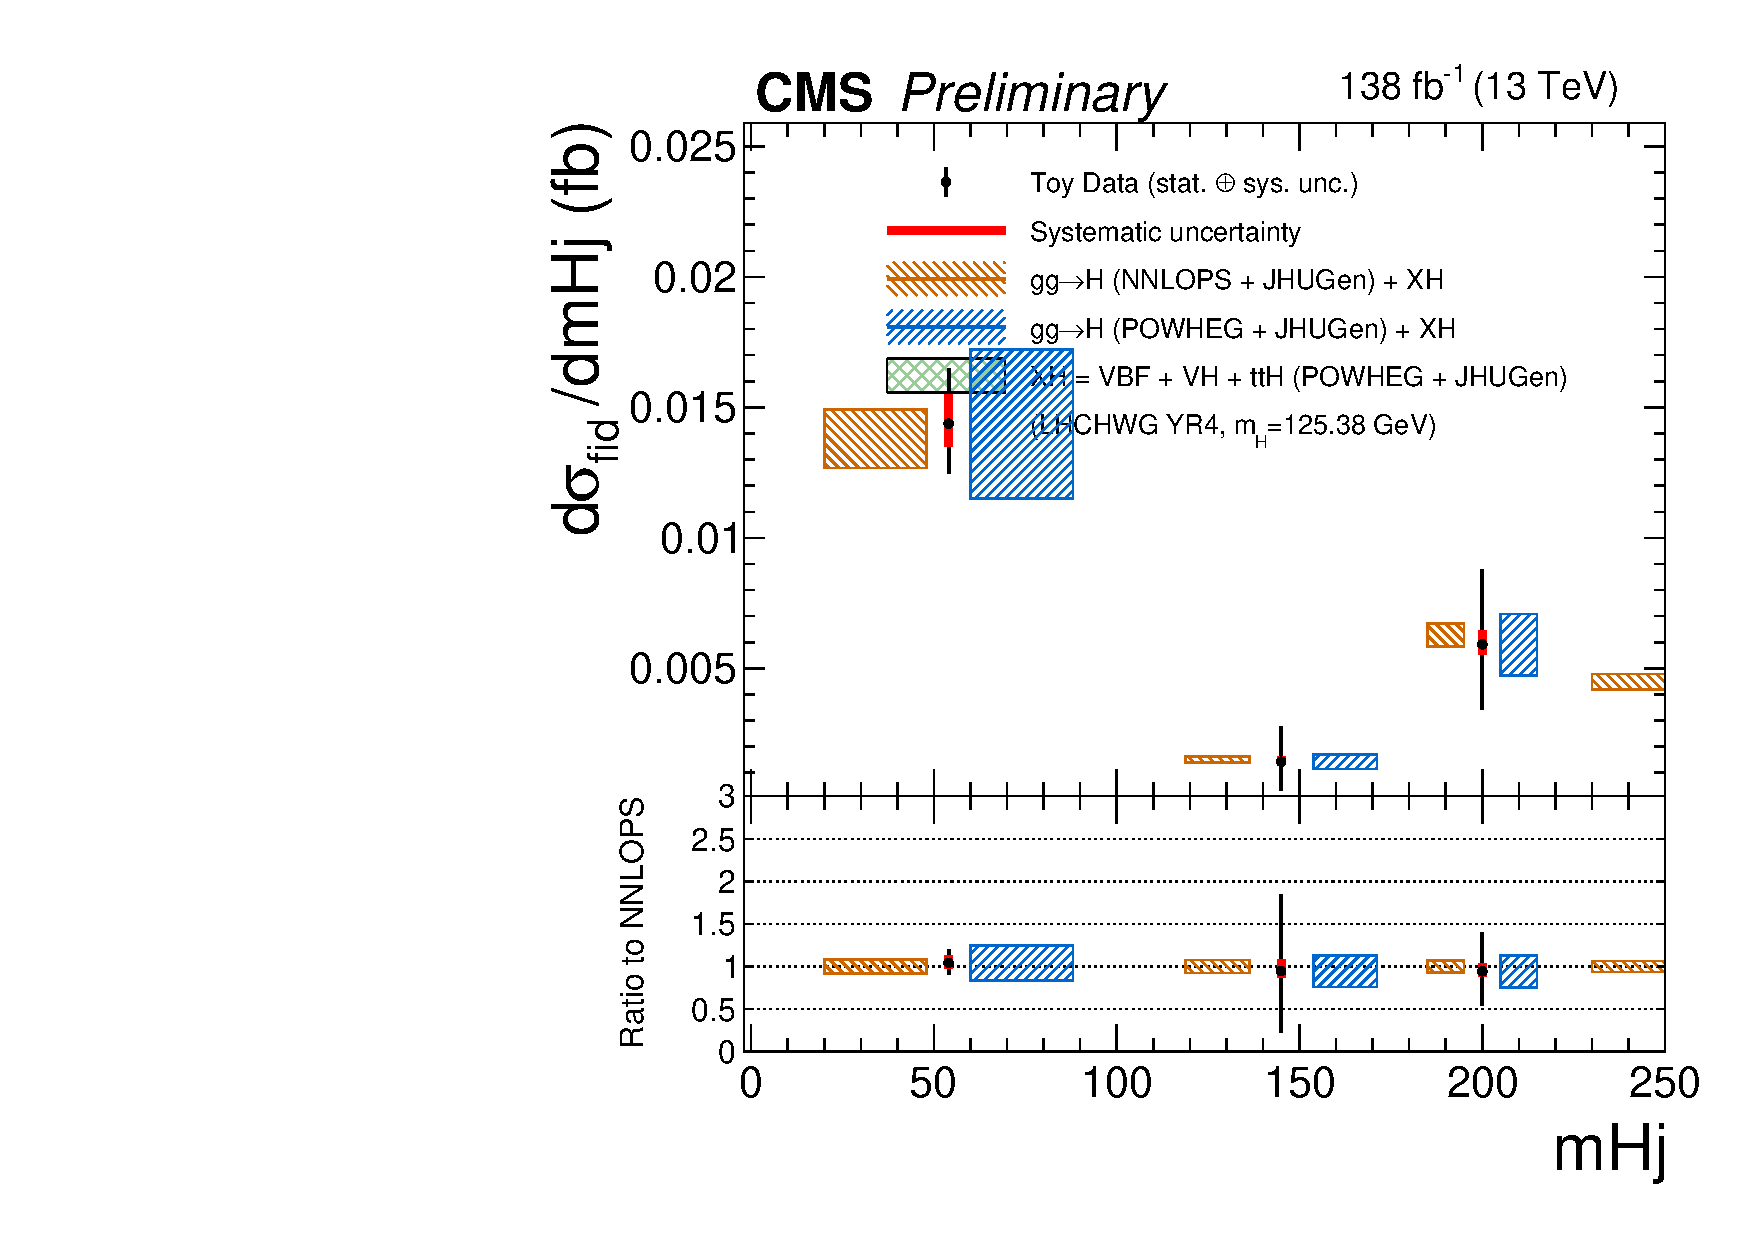
\includegraphics[width=0.48\textwidth]{Images/H4L/mHj_unfoldwith_SM_125_asimov.pdf}
		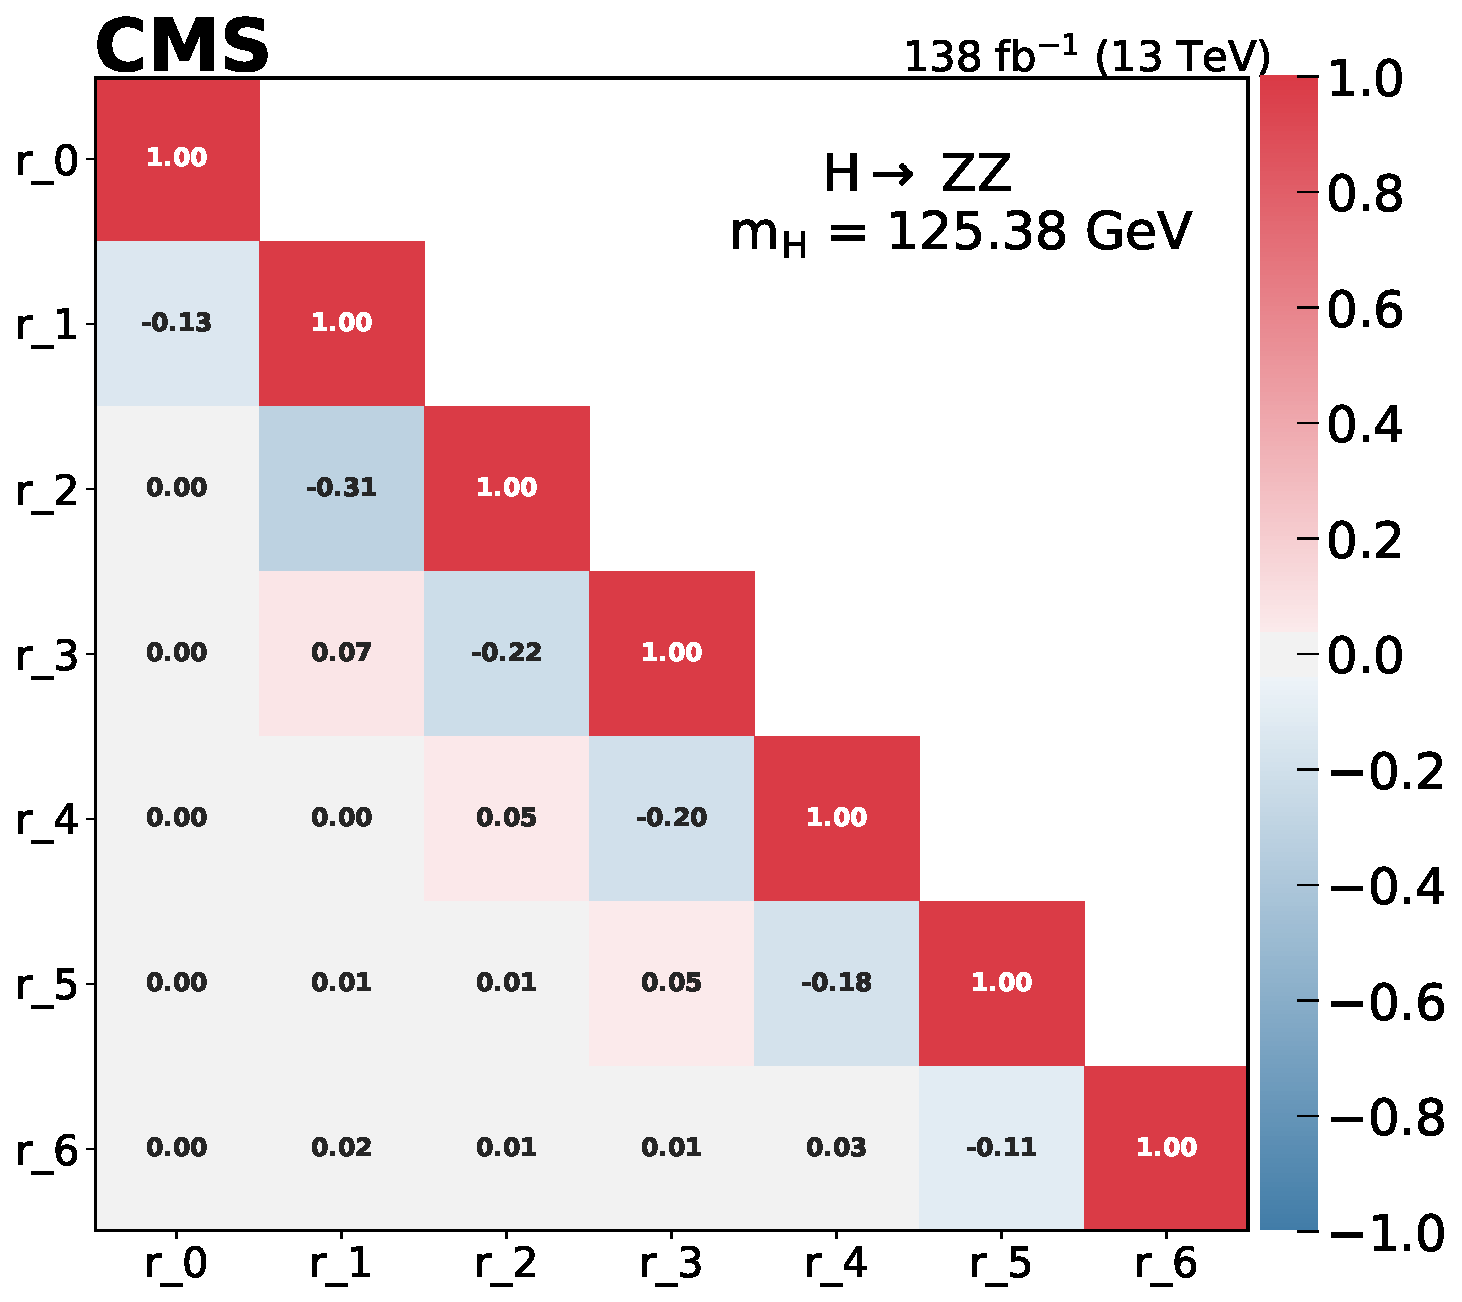
\includegraphics[width=0.48\textwidth]{Images/H4L/correlations/corr_mHj_v3.pdf}\\
		\caption{
			Differential cross sections as a function of the invariant mass of the \PH+leading-jet system $m_{\PH j}$ (left) and the correlation matrix between the observed differential cross sections (right).
			The first bin comprises all those events with less than one jet, for which $m_{\PH j}$  is undefined.
			The acceptance and theoretical uncertainties in the differential bins are calculated using the \POWHEG (blue), NNLOPS (orange), and MadGraph\_aMC@NLO (pink) generators.
			The sub-dominant component of the signal ($\VBF + \VH + \ttH$) is denoted as XH and it is fixed to the SM.
			\label{fig:fidMHJ}}
	\end{figure}
\end{center}

\clearpage

\begin{center}
	\begin{figure}[!htb]
		\centering
		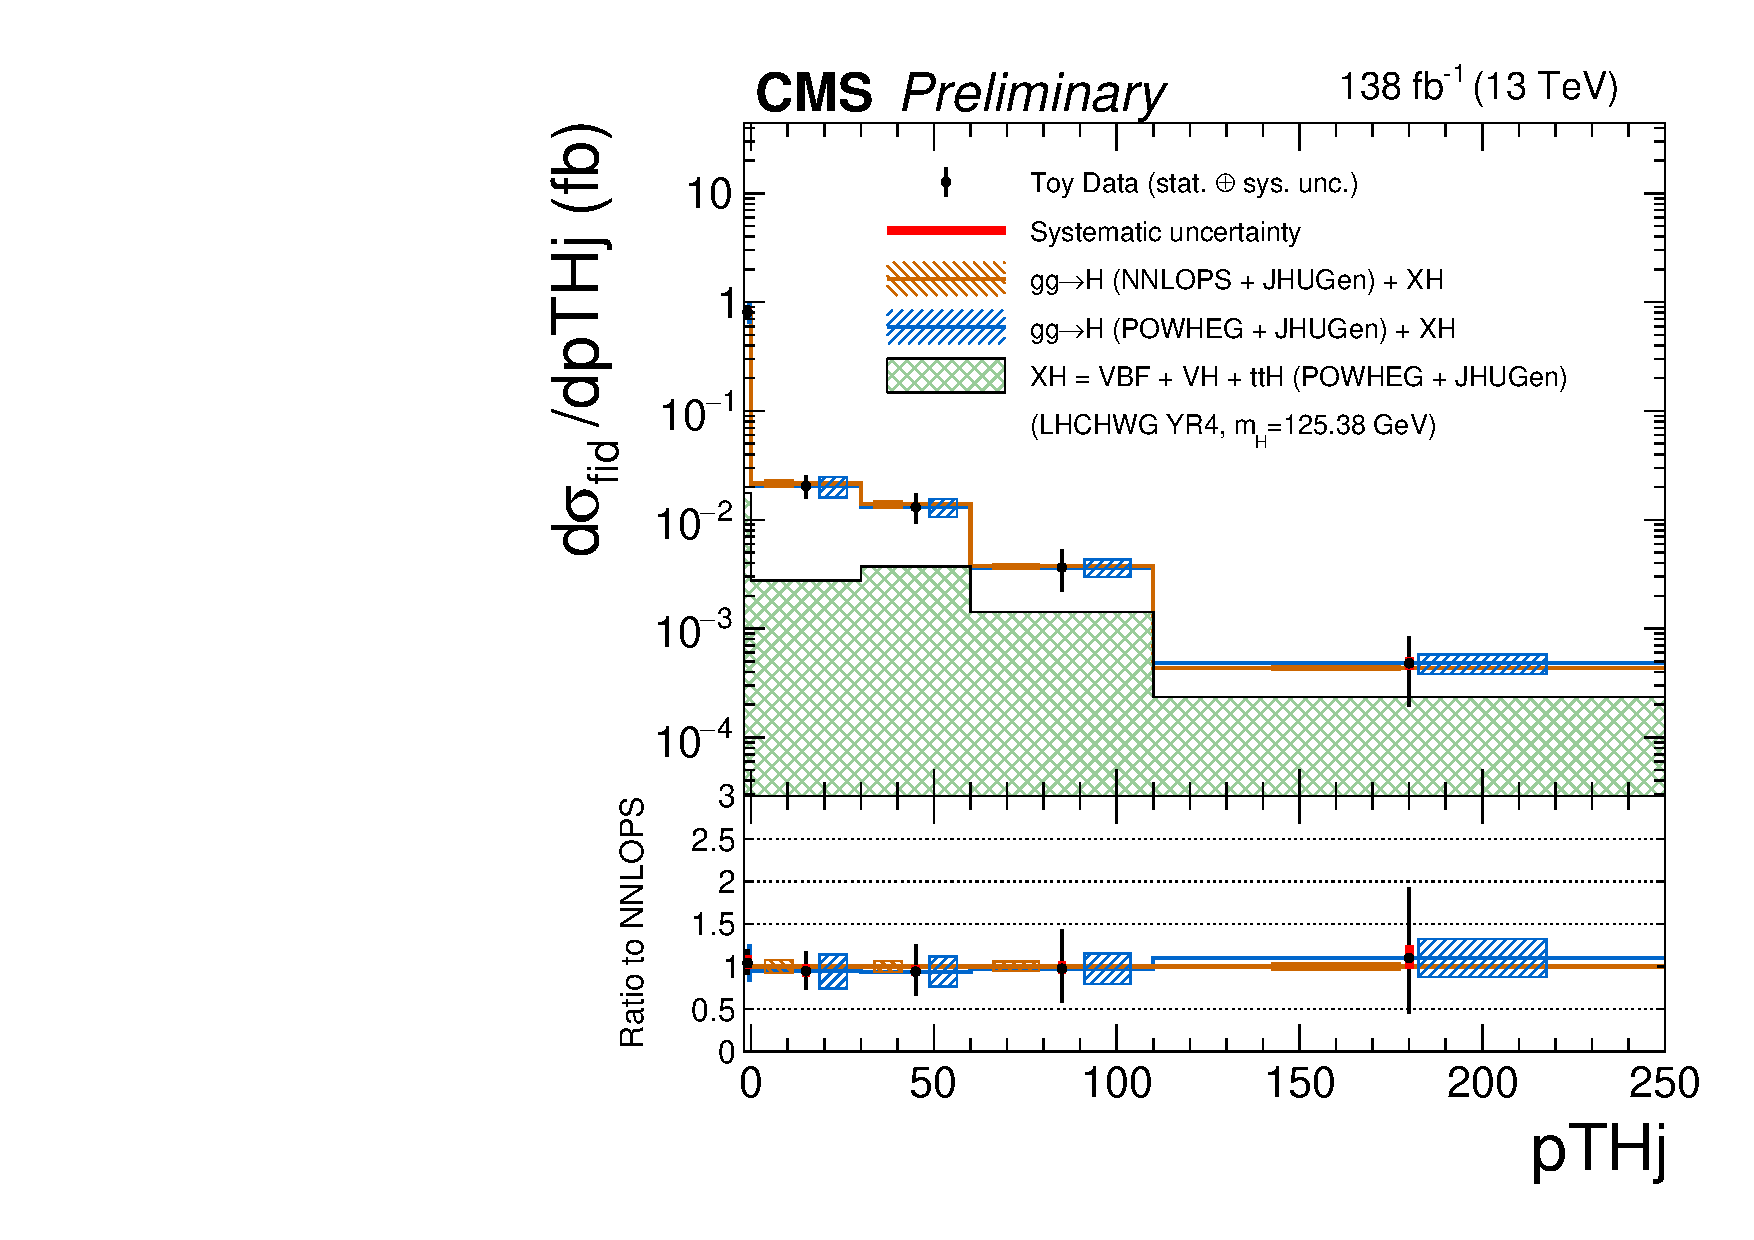
\includegraphics[width=0.48\textwidth]{Images/H4L/pTHj_unfoldwith_SM_125_logscale_asimov.pdf}
		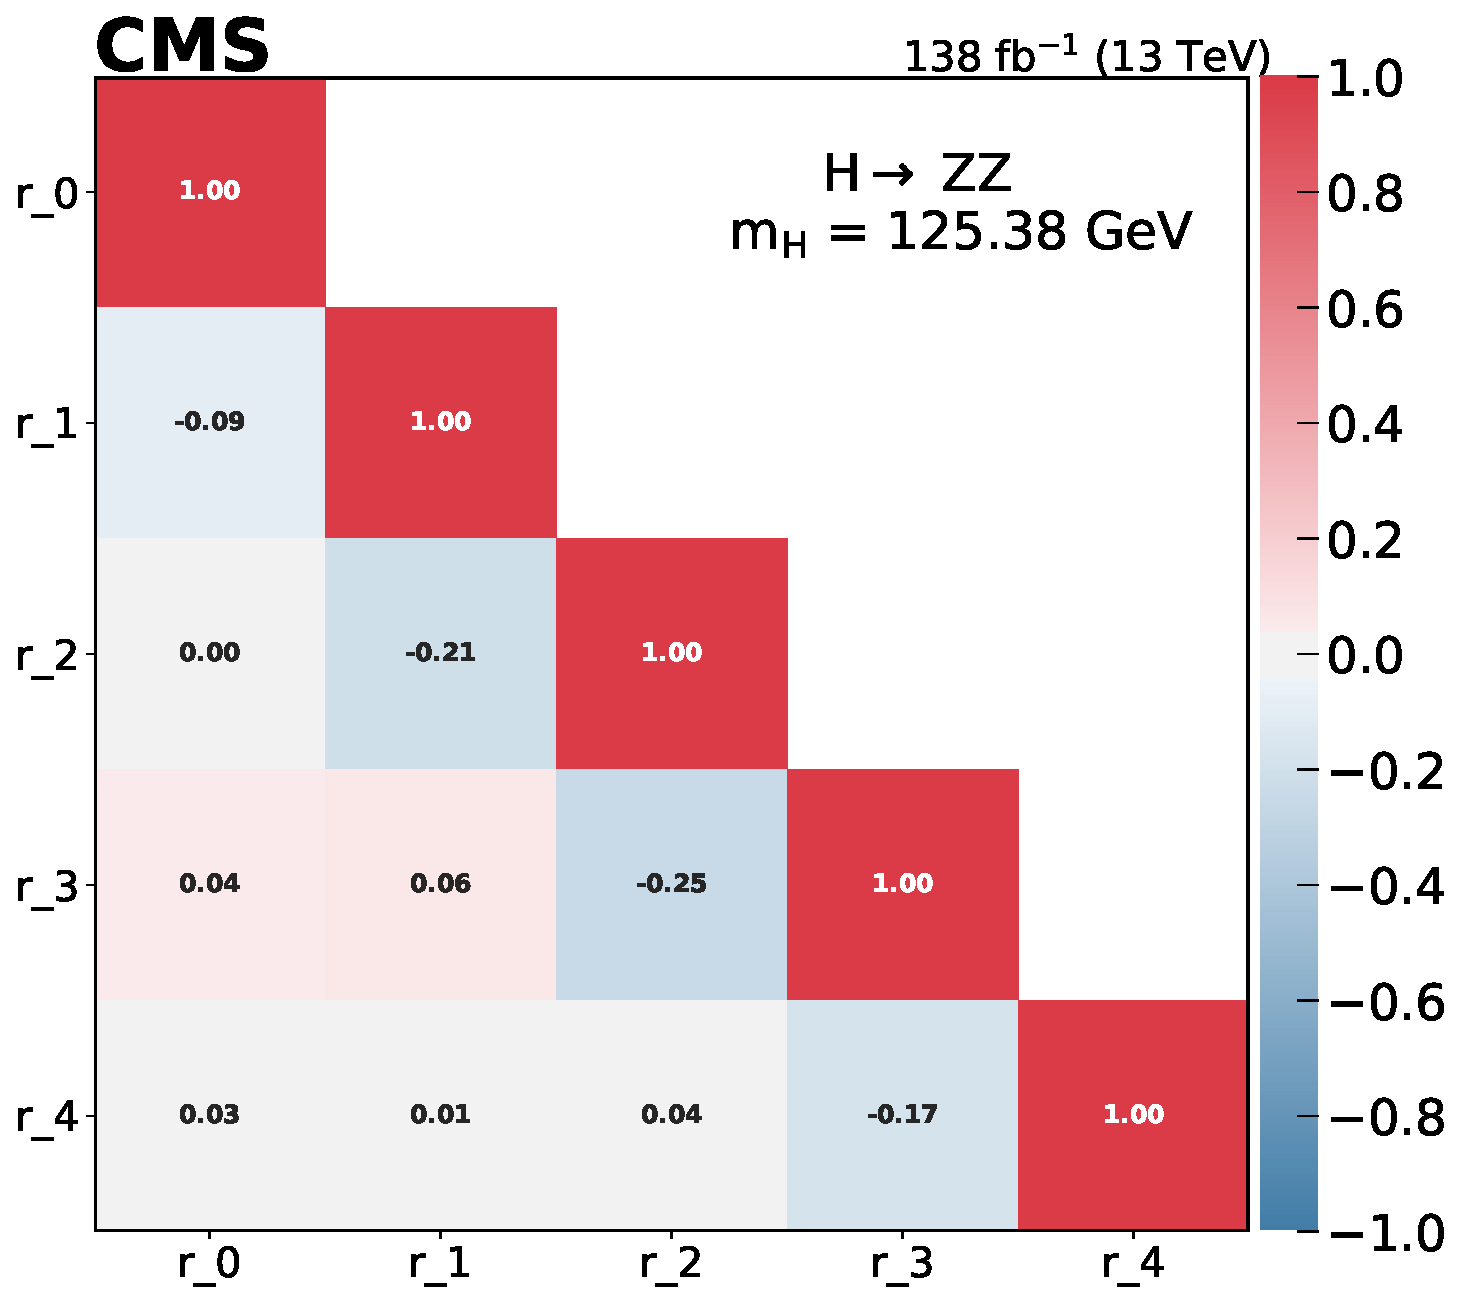
\includegraphics[width=0.48\textwidth]{Images/H4L/correlations/corr_pTHj_v3.pdf}\\
		\caption{
			Differential cross sections as a function of the transverse momentum of the \PH+leading-jet system $\pt^{\PH j}$ (left) and the correlation matrix between the observed differential cross sections (right).
			The first bin comprises all those events with less than one jet, for which $\pt^{\PH j}$  is undefined.
			The acceptance and theoretical uncertainties in the differential bins are calculated using the \POWHEG (blue), NNLOPS (orange), and MadGraph\_aMC@NLO (pink) generators.
			The sub-dominant component of the signal ($\VBF + \VH + \ttH$) is denoted as XH and it is fixed to the SM.
			\label{fig:fidPTHJ}}
	\end{figure}
\end{center}

\clearpage

%\begin{center}
%\begin{figure}[!htb]
%	\centering
%	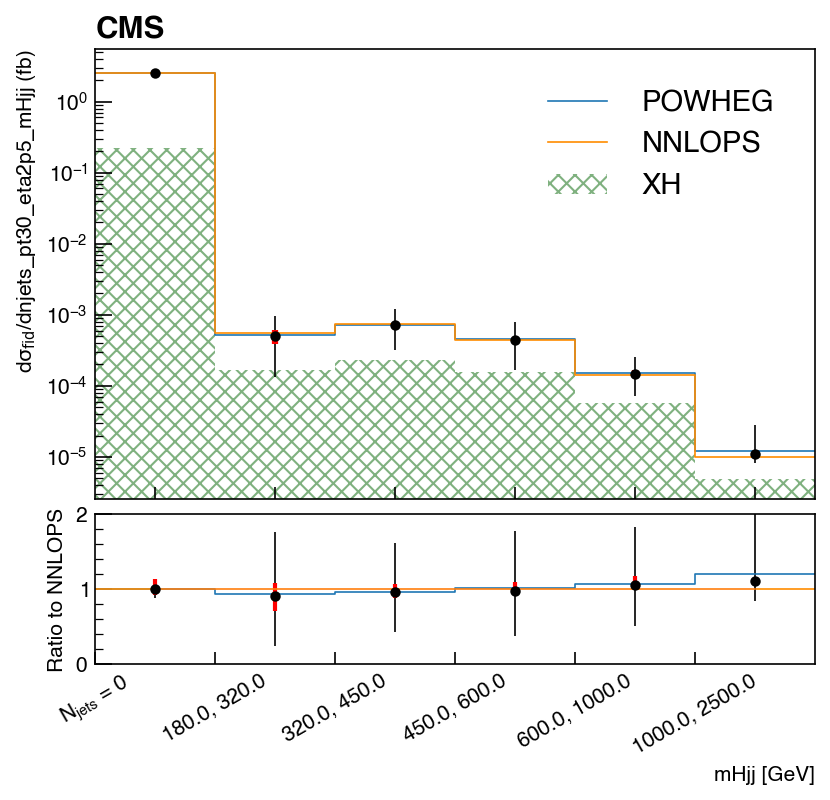
\includegraphics[width=0.48\textwidth]{Images/H4L/plot_njets_pt30_eta2p5_mHjj.png}
%	\includegraphics[width=0.48\textwidth]{Images/H4L/correlations/corr_mHjj_v3.pdf}\\
%	\caption{
	%		Differential cross sections as a function of  $m_{\PH jj}$.
	%		The acceptance and theoretical uncertainties in the differential bins are calculated using \POWHEG.
	%		The sub-dominant component of the signal ($\VBF + \VH + \ttH$) is denoted as XH.
	%		\label{fig:fidMHJJ}}
%\end{figure}
%\end{center}

\begin{center}
	\begin{figure}[!htb]
		\centering
		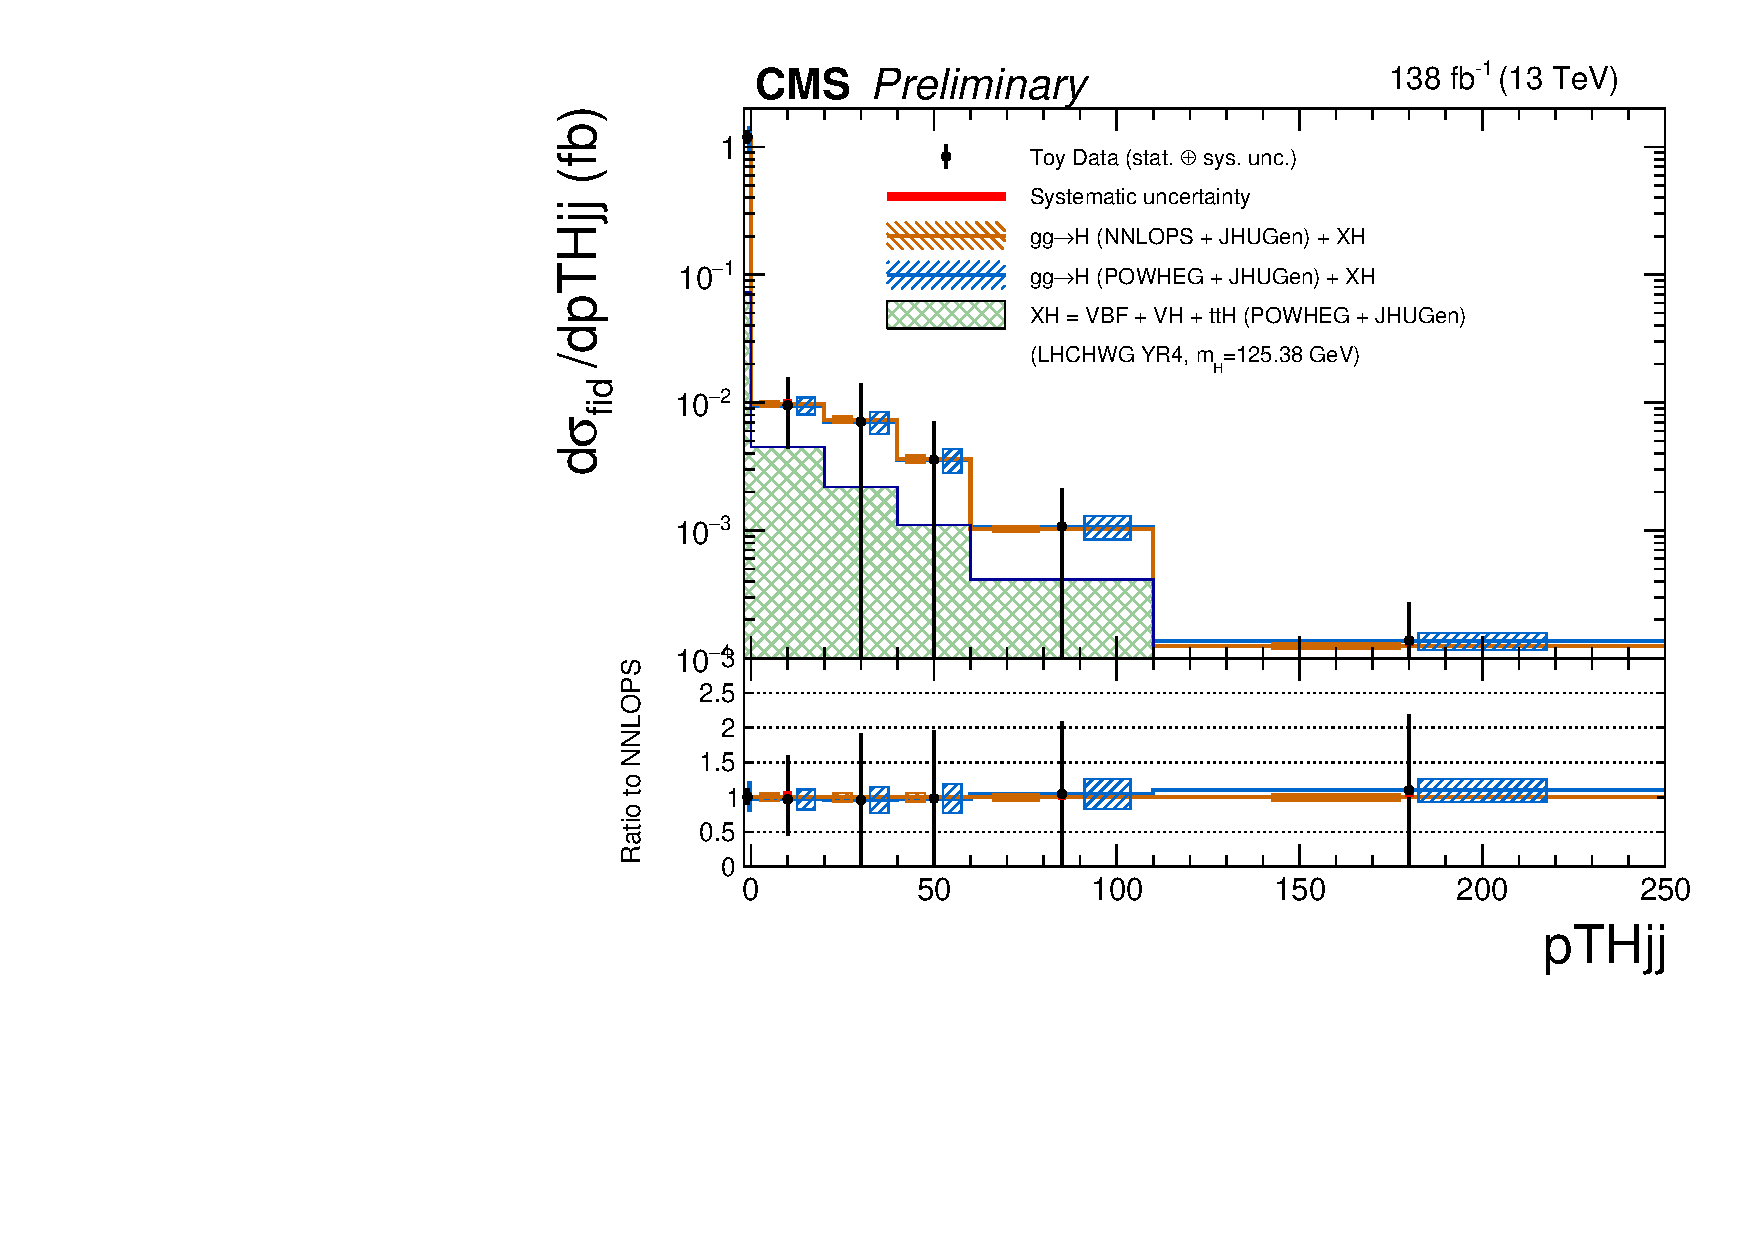
\includegraphics[width=0.48\textwidth]{Images/H4L/pTHjj_unfoldwith_SM_125_asimov.pdf}
		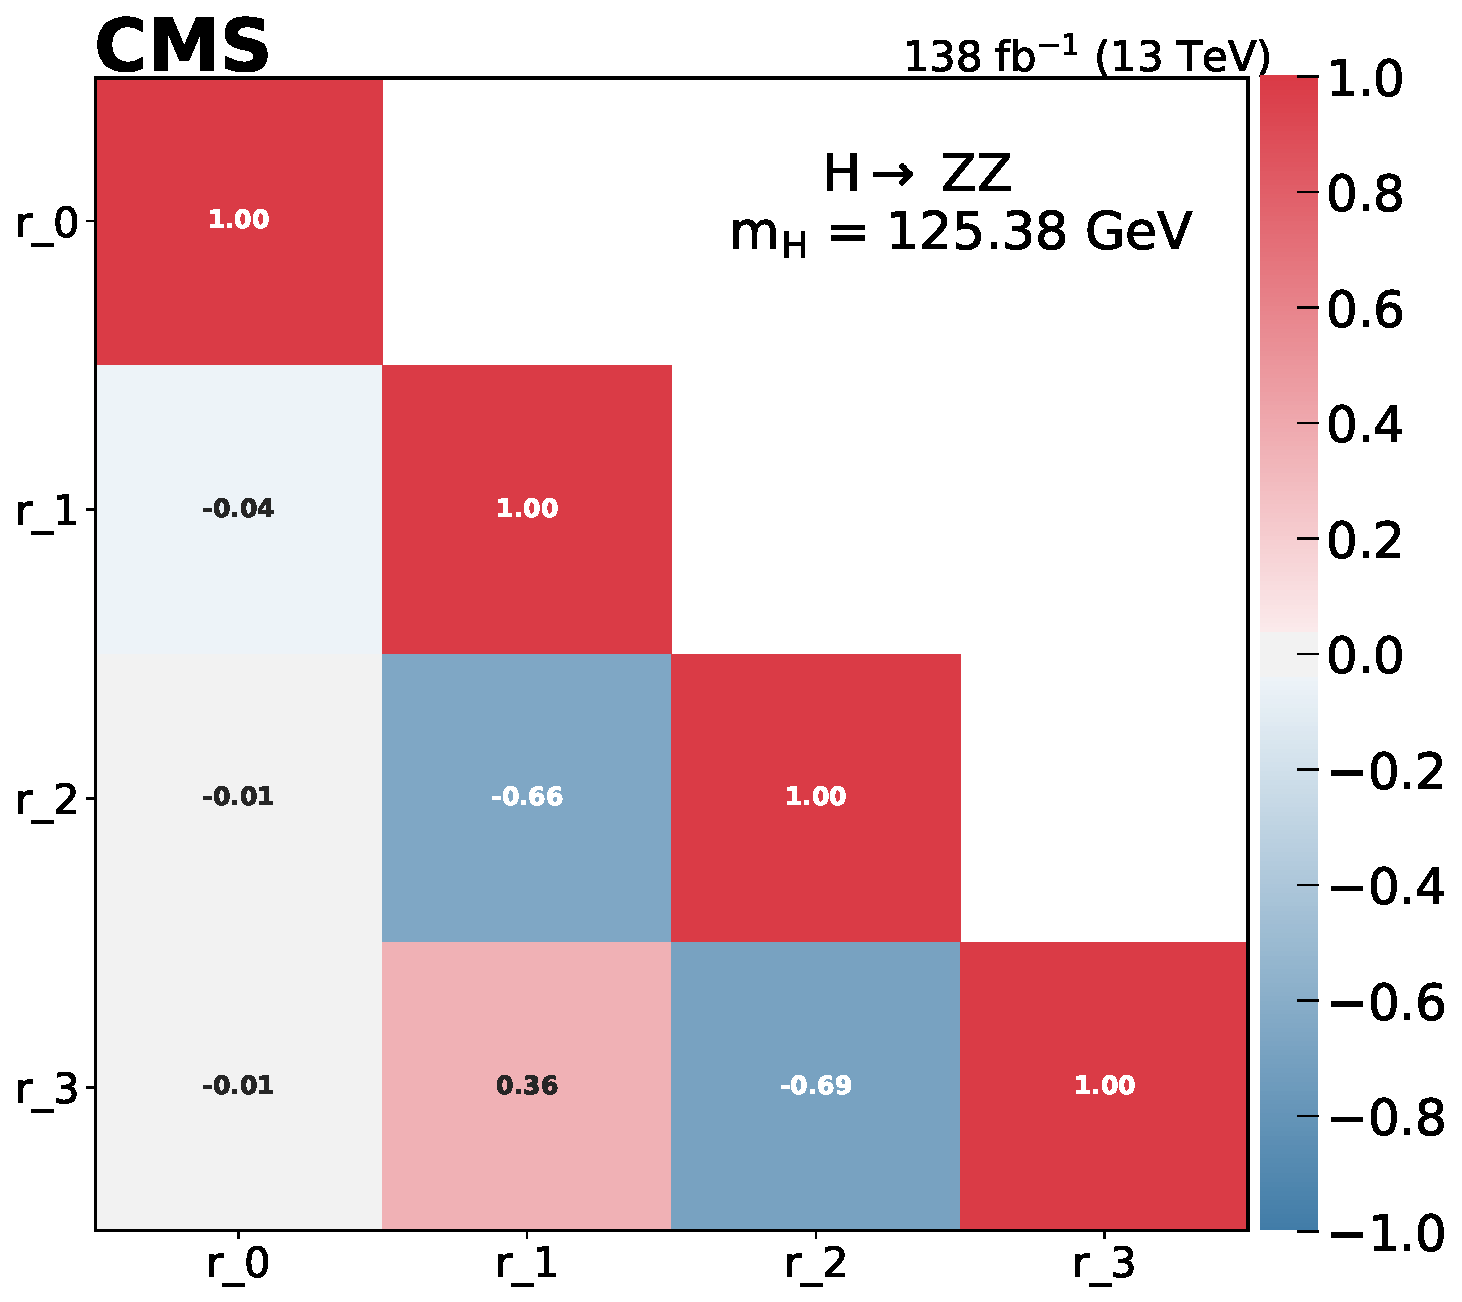
\includegraphics[width=0.48\textwidth]{Images/H4L/correlations/corr_pTHjj_v3.pdf}\\
		\caption{
			Differential cross sections as a function of the transverse momentum of the \PH+di-jet system $\pt^{\PH jj}$ (left) and the correlation matrix between the observed differential cross sections (right).
			The first bin comprises all those events with less than two jet, for which $\pt^{\PH jj}$  is undefined.
			The acceptance and theoretical uncertainties in the differential bins are calculated using the \POWHEG (blue), NNLOPS (orange), and MadGraph\_aMC@NLO (pink) generators.
			The sub-dominant component of the signal ($\VBF + \VH + \ttH$) is denoted as XH and it is fixed to the SM.
			\label{fig:fidPTHJJ}}
	\end{figure}
\end{center}

\clearpage

%%%%%%%%%%%%%%%%%%%%%%%% Jet Veto T_B,C %%%%%%%%%%%%%%%%%%%%%%%%%

\begin{center}
	\begin{figure}[!htb]
		\centering
		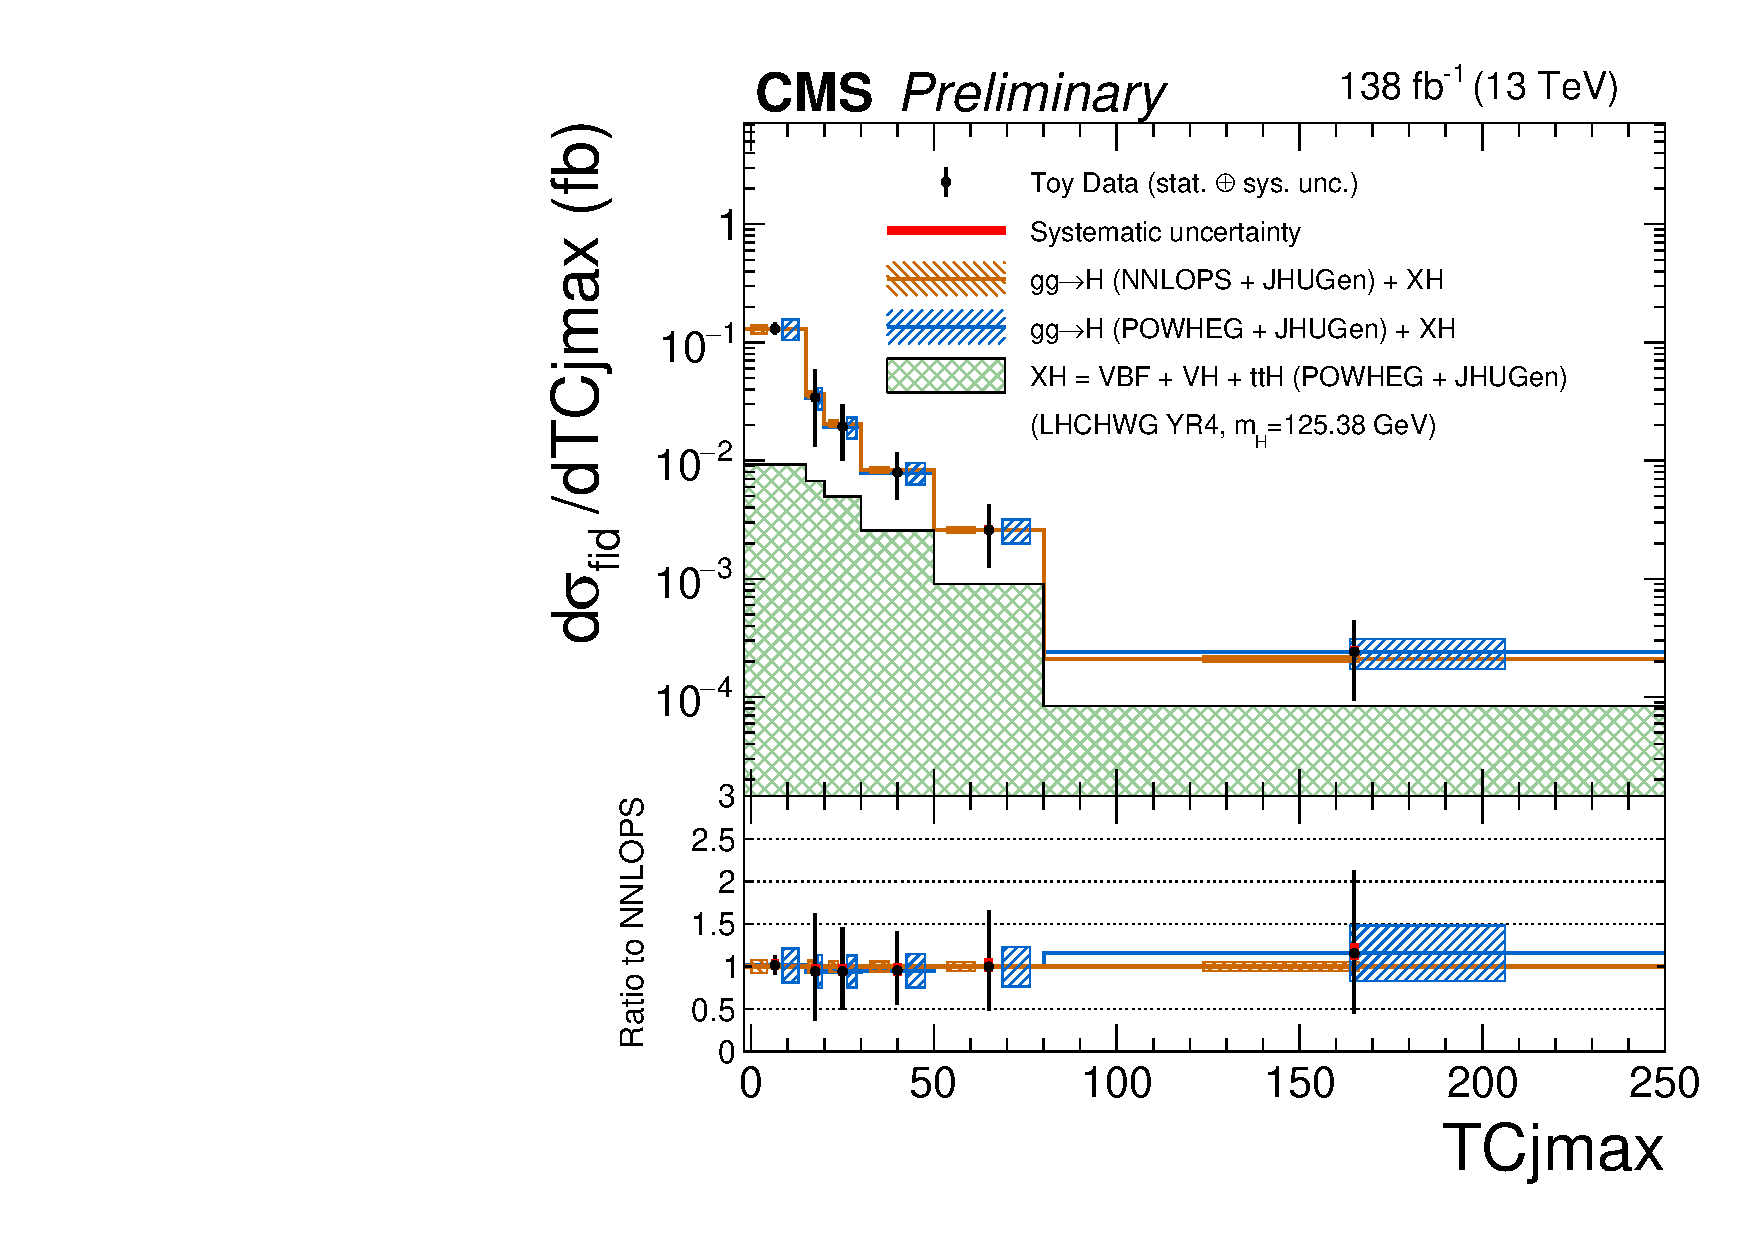
\includegraphics[width=0.48\textwidth]{Images/H4L/TCjmax_unfoldwith_SM_125_logscale_asimov.pdf}
		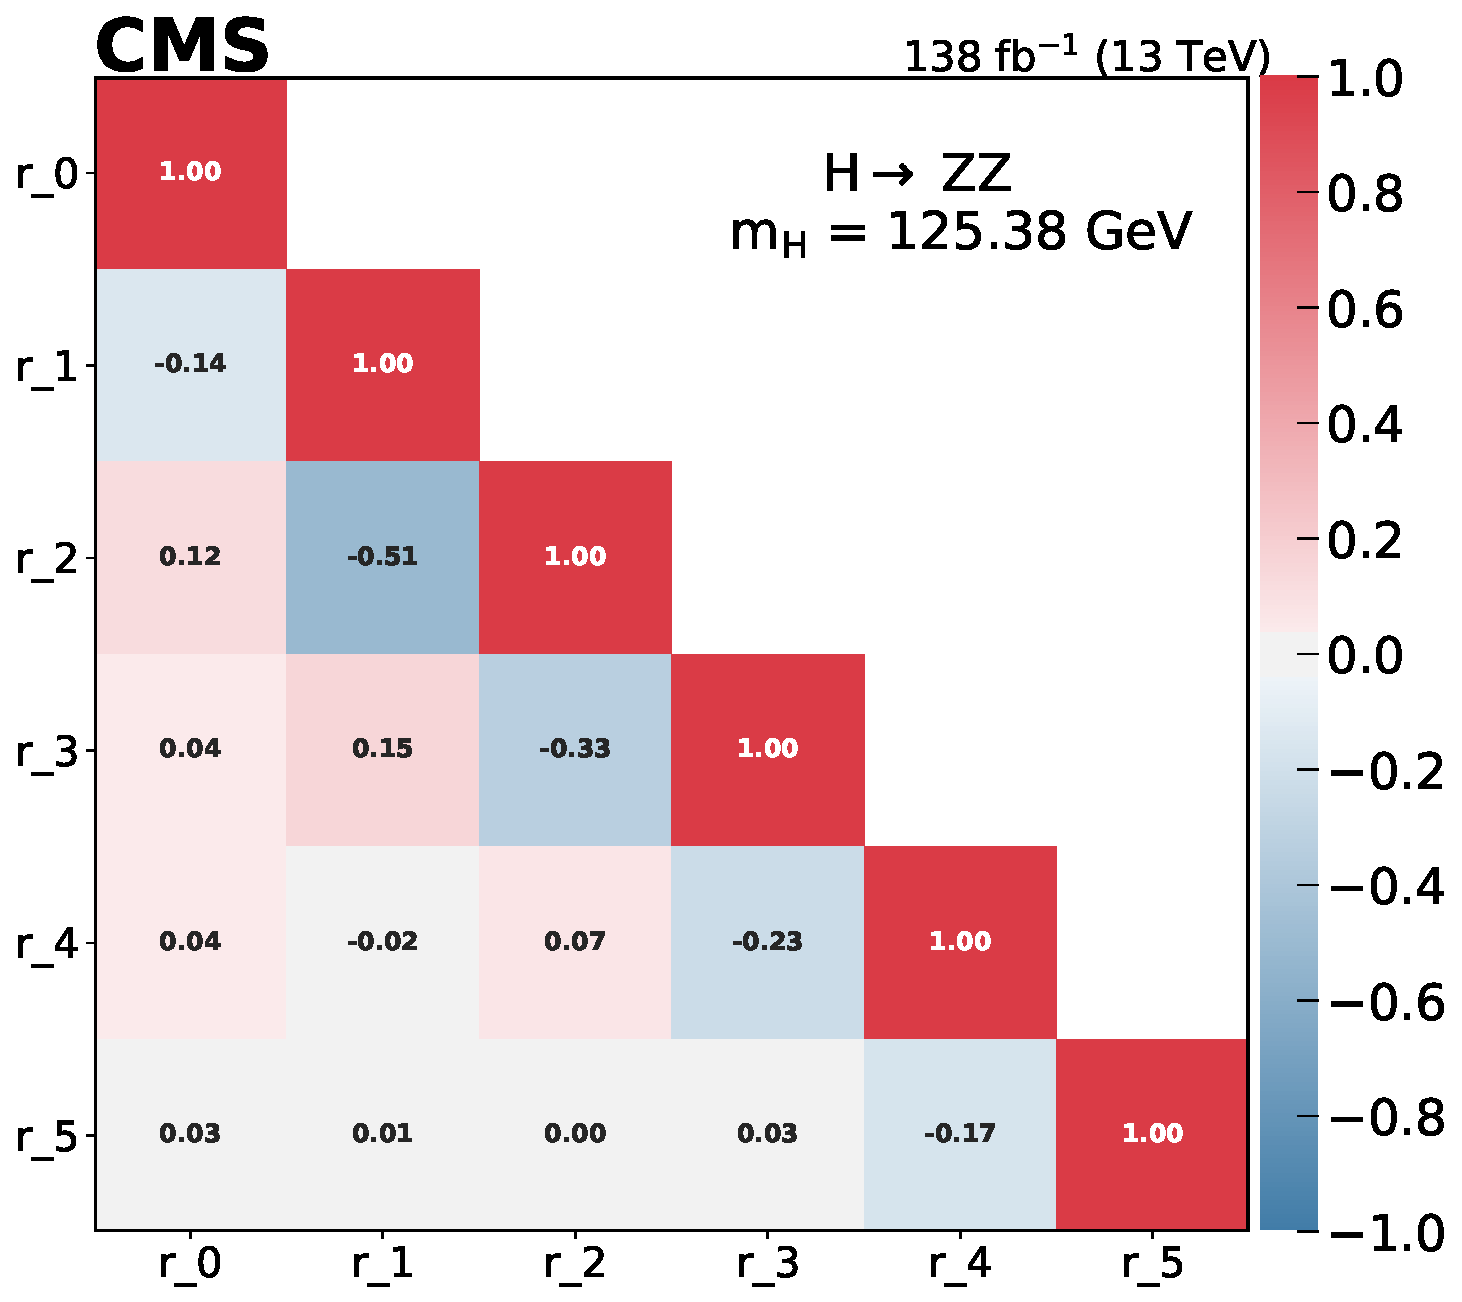
\includegraphics[width=0.48\textwidth]{Images/H4L/correlations/corr_TCjmax_v3.pdf}\\
		\caption{
			Differential cross sections as a function of the rapidity-weighed jet veto $\mathcal{T}_{\text{C}}$ (left) and the correlation matrix between the observed differential cross sections (right).
			The first bin comprises all those events with less than one jet, for which $\mathcal{T}_{\text{C}}$ is undefined.
			The acceptance and theoretical uncertainties in the differential bins are calculated using the \POWHEG (blue), NNLOPS (orange), and MadGraph\_aMC@NLO (pink) generators.
			The sub-dominant component of the signal ($\VBF + \VH + \ttH$) is denoted as XH and it is fixed to the SM.
			\label{fig:fidTC}}
	\end{figure}
\end{center}

\clearpage

\begin{center}
	\begin{figure}[!htb]
		\centering
		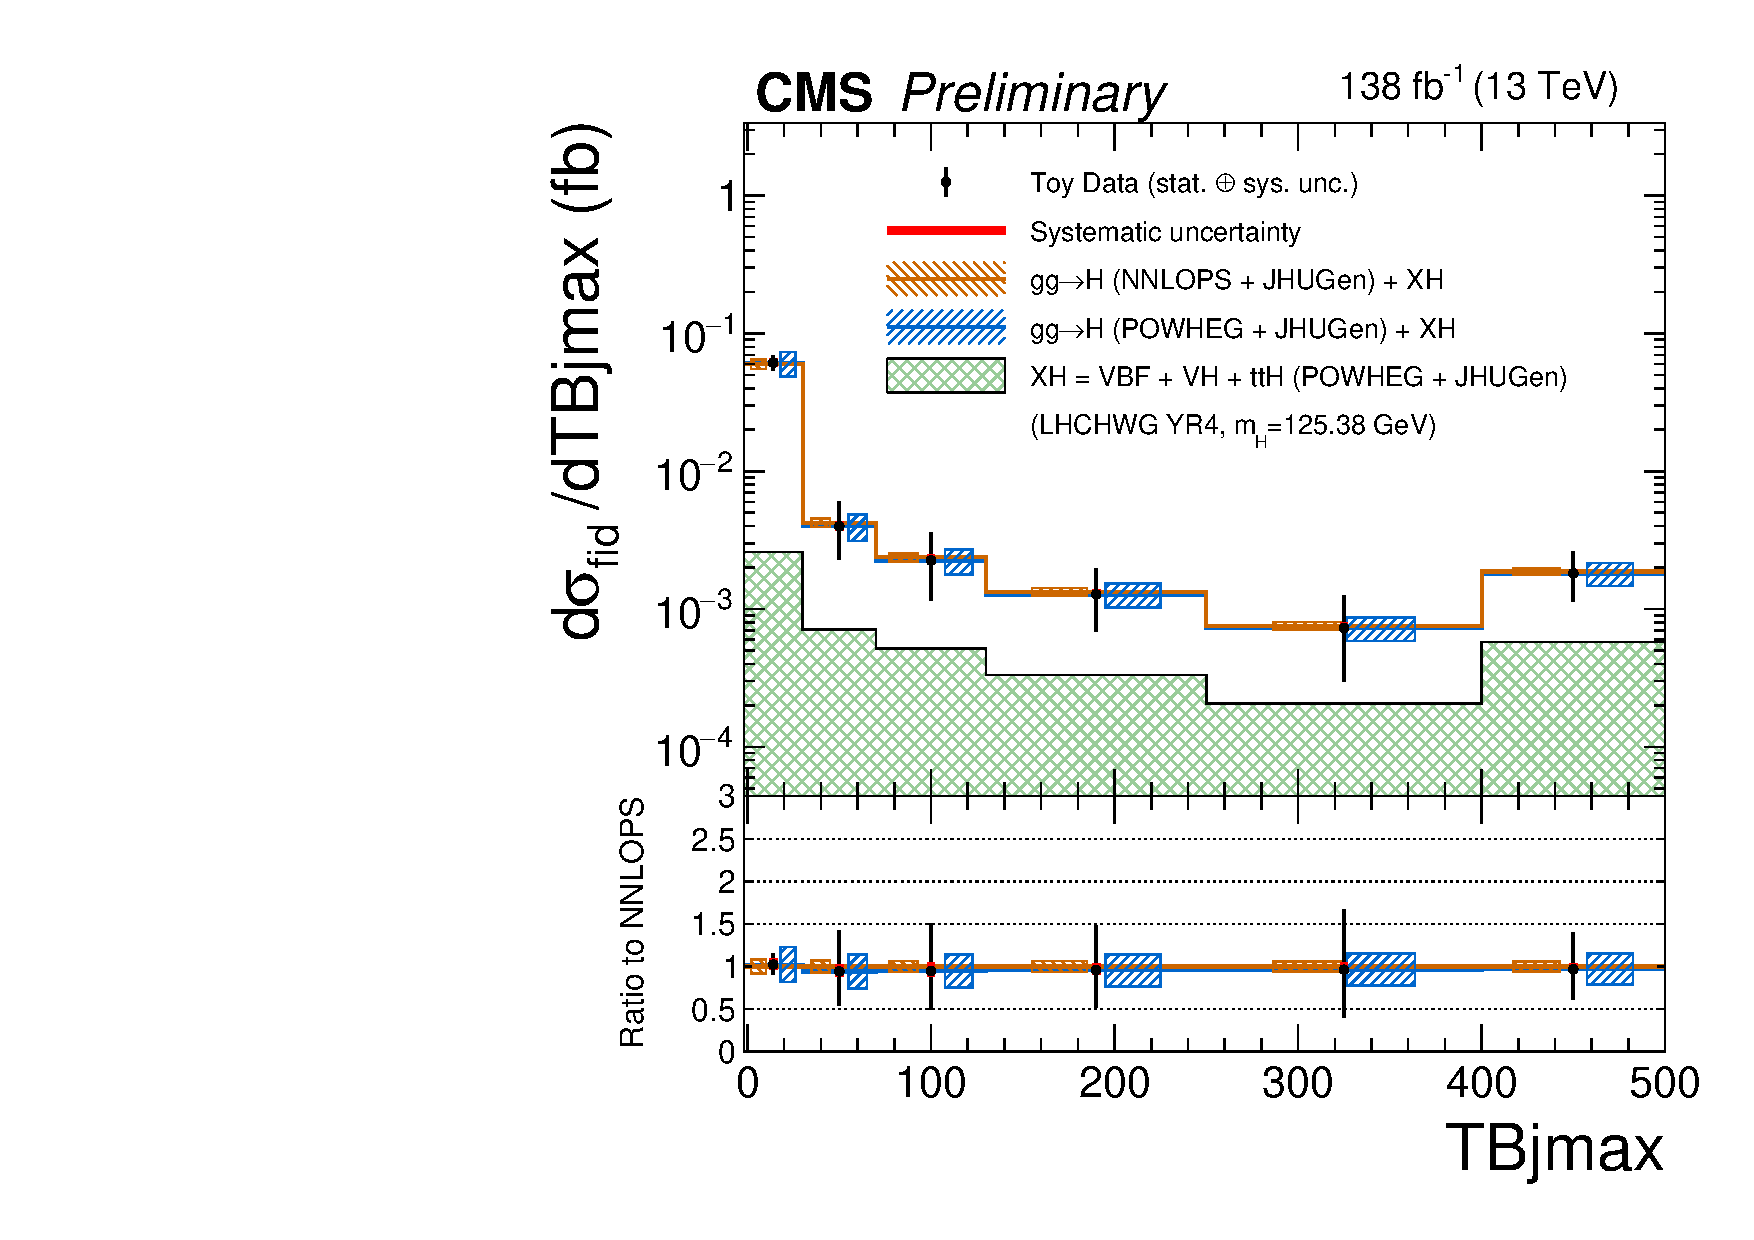
\includegraphics[width=0.48\textwidth]{Images/H4L/TBjmax_unfoldwith_SM_125_logscale_asimov.pdf}
		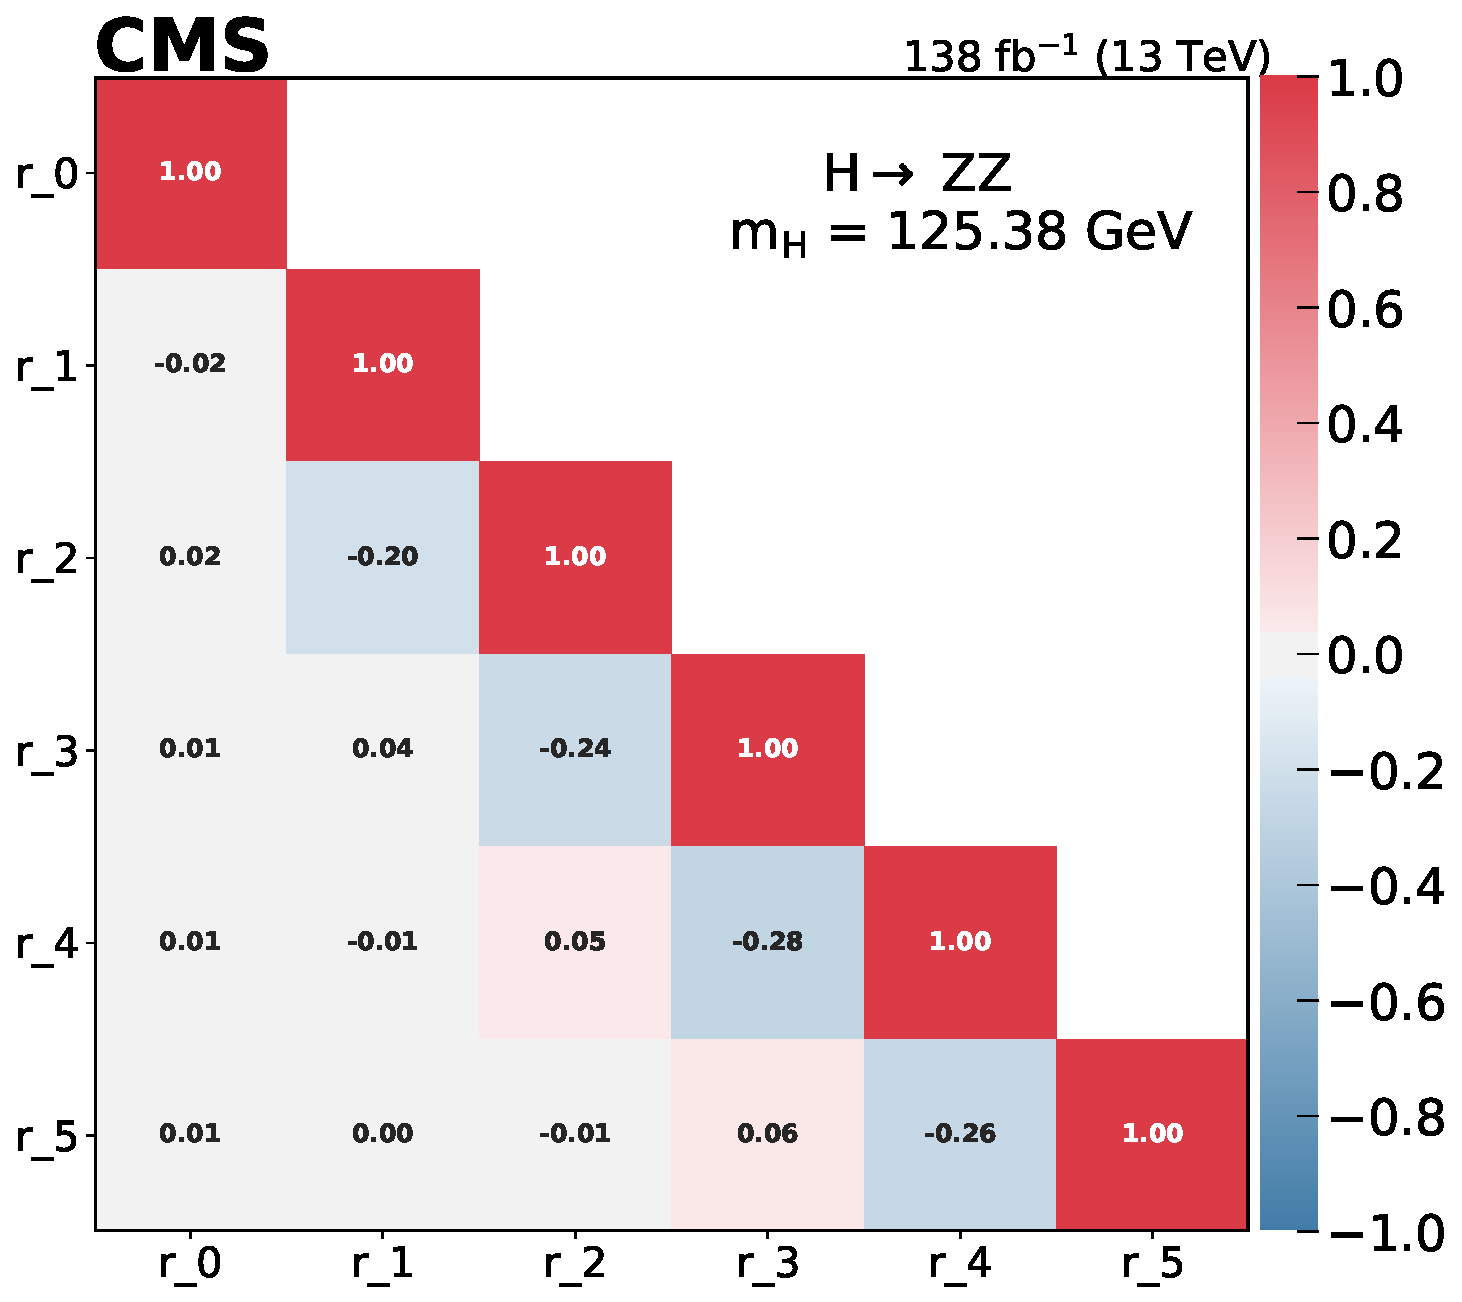
\includegraphics[width=0.48\textwidth]{Images/H4L/correlations/corr_TBjmax_v3.pdf}\\
		\caption{
			Differential cross sections as a function of the rapidity-weighed jet veto $\mathcal{T}_{\text{B}}$ (left) and the correlation matrix between the observed differential cross sections (right).
			The first bin comprises all those events with less than one jet, for which $\mathcal{T}_{\text{B}}$ is undefined.
			The acceptance and theoretical uncertainties in the differential bins are calculated using the \POWHEG (blue), NNLOPS (orange), and MadGraph\_aMC@NLO (pink) generators.
			The sub-dominant component of the signal ($\VBF + \VH + \ttH$) is denoted as XH and it is fixed to the SM.
			\label{fig:fidTB}}
	\end{figure}
\end{center}

\clearpage

\subsection{Differential cross sections: decay}
One of the distinguishing features of the $\Hllll$ decay is the composition of the final state, where intereference effects between the same flavour and different flavours final states are present.
To resolve these effects and therefore enhance the model independence of the results, the measurements of the differential cross sections in bins of kinematic observables sensitive to the $\Hllll$ decay are measured separately for the same and different flavour final states.

The cross sesctions measured in bins of the invariant mass of the two \PZ boson candidates in the event are shown in Fig.\ref{fig:fidMZ1} and \ref{fig:fidMZ2}, respectively.
As discussed in Sec.~\ref{sec:observables}, the $\Hllll$ decay is completely defined by seven degrees of freedom, two of which are the invariant masses of the two \PZ boson candidates in the event. The measurement of the differential cross sections in bins of these two observables are shown in Fig.\ref{fig:fidMZ1} and \ref{fig:fidMZ2}, respectively.
The additional five degrees of freedom are the angles that characterise the decay of the \PH boson and the planes that contain the two \PZ bosons produced. 
The angle $\theta^\star$ is defined as the angle between the beam axis and the direction of the $\PZ_1$ candidate in the event, while the angles between the $\PZ_1$ and $\PZ_2$ flight directions and the planes containing the di-lepton systems originating from their decay are denoted as  $\theta_1$ and $\theta_2$.
The measurements in differential bins of the cosine of these angles are presented in Fig.~\ref{fig:fidCOSTS} ,~\ref{fig:fidCOSZ1}, and \ref{fig:fidCOSZ2}, respectively.
The $\phi$ and $\phi_1$ are defined as the angles between the three planes containing the \PH boson and the decay products of the $\PZ_1$ and $\PZ_2$ candidates and the corresponding differential cross sections are presented in Fig.~\ref{fig:fidPHI} and Fig.~\ref{fig:fidPHISTAR}. 

These observables completely characterise the $\Hllll$ decay and can be used to compute matrix element discriminants sensitive to the presence of possible BSM physics. The main advantage of using these discriminants lies in the fact that they fully encapsulate all the information present in the $\Hllll$ decay and are directly sensitive to \PH boson anomalous couplings and CP-violation.

This analysis measures cross sections in differential bins of six kinematic discriminants sensitive to different HVV anomalous couplings and their possible interference: \Dzm, \Dzhp, \DCP, \Dint, \DLone, and \DLoneZg. An more detailed description of these discriminants is given in Sec.~\ref{sec:discriminants} and Ref.~\cite{CMSHIG19009}.
The results of these measurements are shown in Fig.~\ref{fig:fidDZM}, \ref{fig:fidDOHP}, \ref{fig:fidDCP}, \ref{fig:fidDINT}, \ref{fig:fidDL1}, and \ref{fig:fidDL1ZG}.

\clearpage

\begin{center}
	\begin{figure}[!htb]
		\centering
		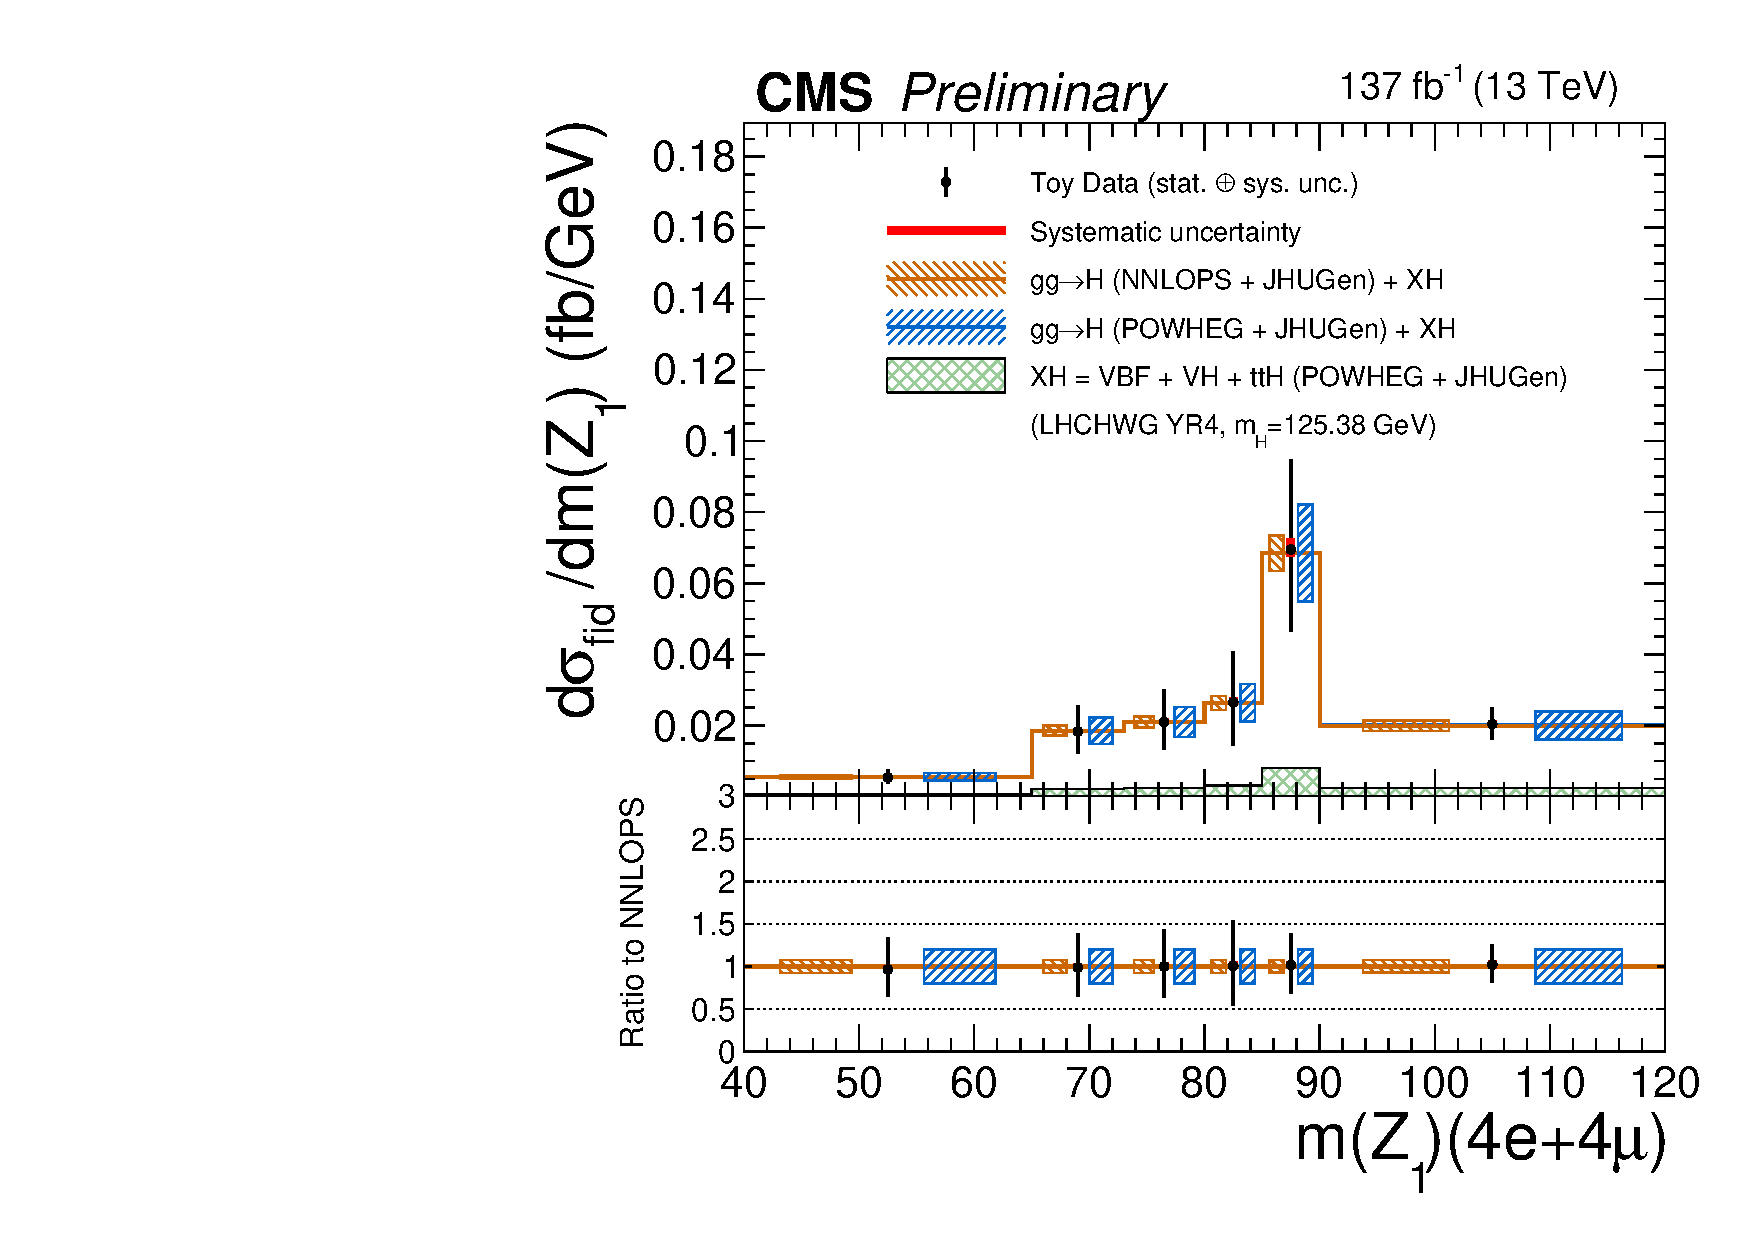
\includegraphics[width=0.48\textwidth]{Images/H4L/ZCands/model_v4/massZ1_unfoldwith_4l_SM_125_asimov.pdf}
		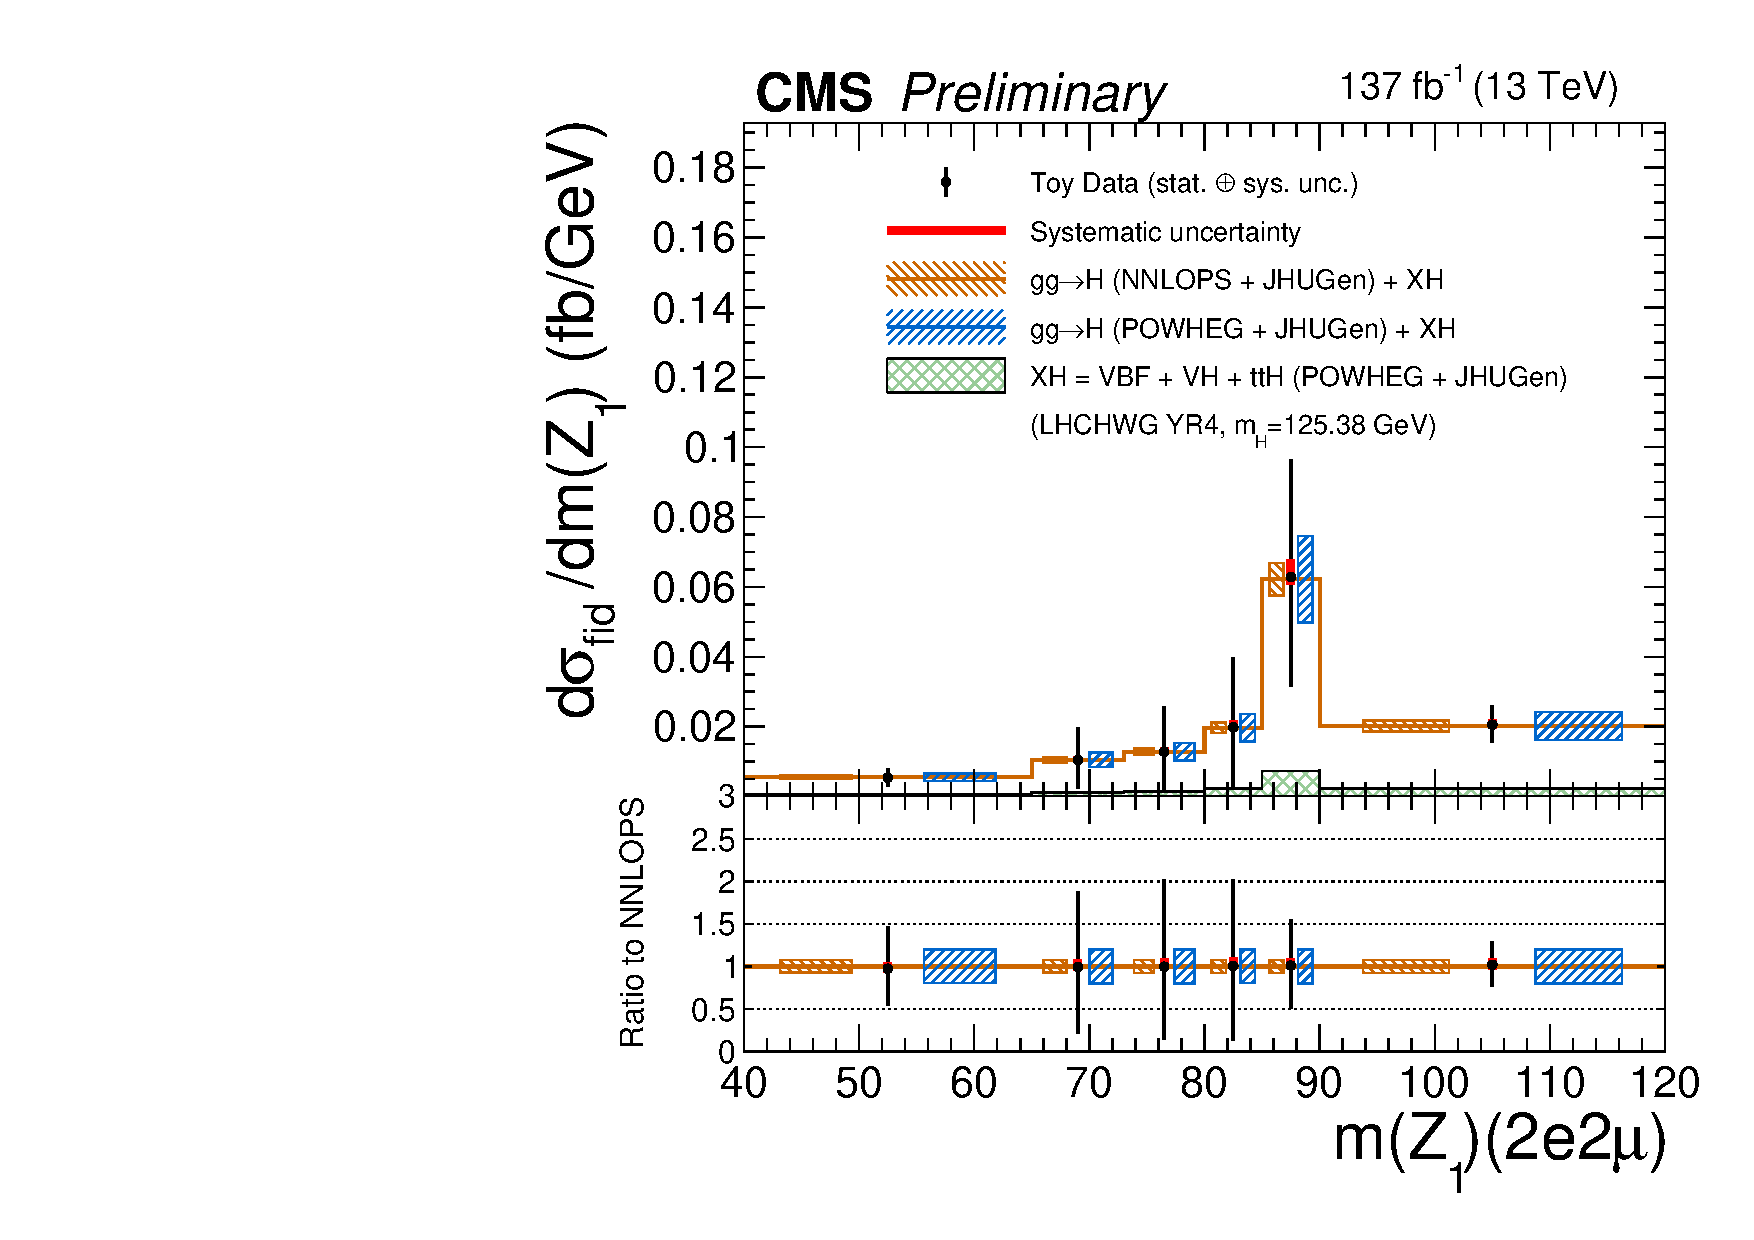
\includegraphics[width=0.48\textwidth]{Images/H4L/ZCands/model_v4/massZ1_unfoldwith_2e2mu_SM_125_asimov.pdf}\\
		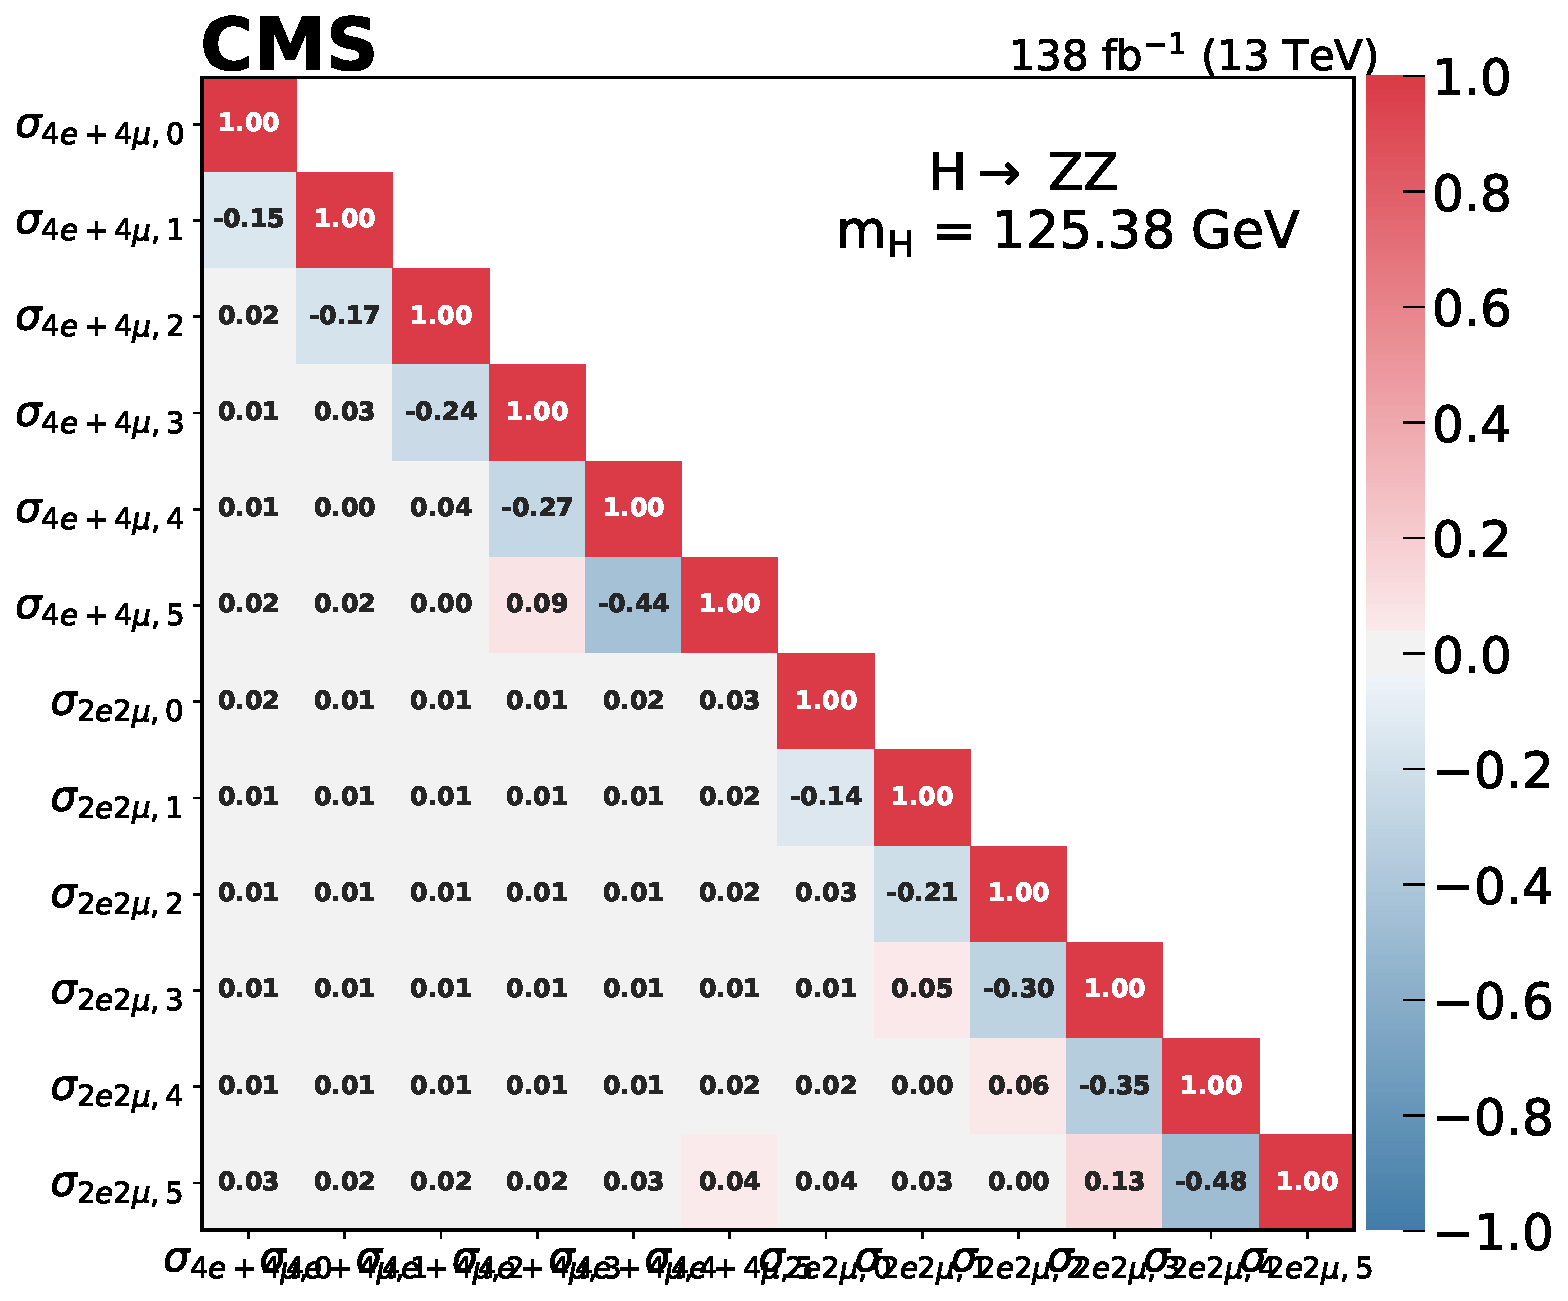
\includegraphics[width=0.48\textwidth]{Images/H4L/correlations/corr_massZ1_v4.pdf}\\	
		\caption{
			Differential cross sections as a function of the invariant mass of the leading di-lepton pair $m_{\PZ_{1}}$ in the same-flavor (top left) and opposite-flavor (top right)  final states.
			The bottom plot shows the correlation matrix between the observed differential cross sections.
			The acceptance and theoretical uncertainties in the differential bins are calculated using the \POWHEG (blue), NNLOPS (orange), and MadGraph\_aMC@NLO (pink) generators.
			The sub-dominant component of the signal ($\VBF + \VH + \ttH$) is denoted as XH and it is fixed to the SM.
			\label{fig:fidMZ1}}
	\end{figure}
\end{center}

\clearpage

\begin{center}
	\begin{figure}[!htb]
		\centering
		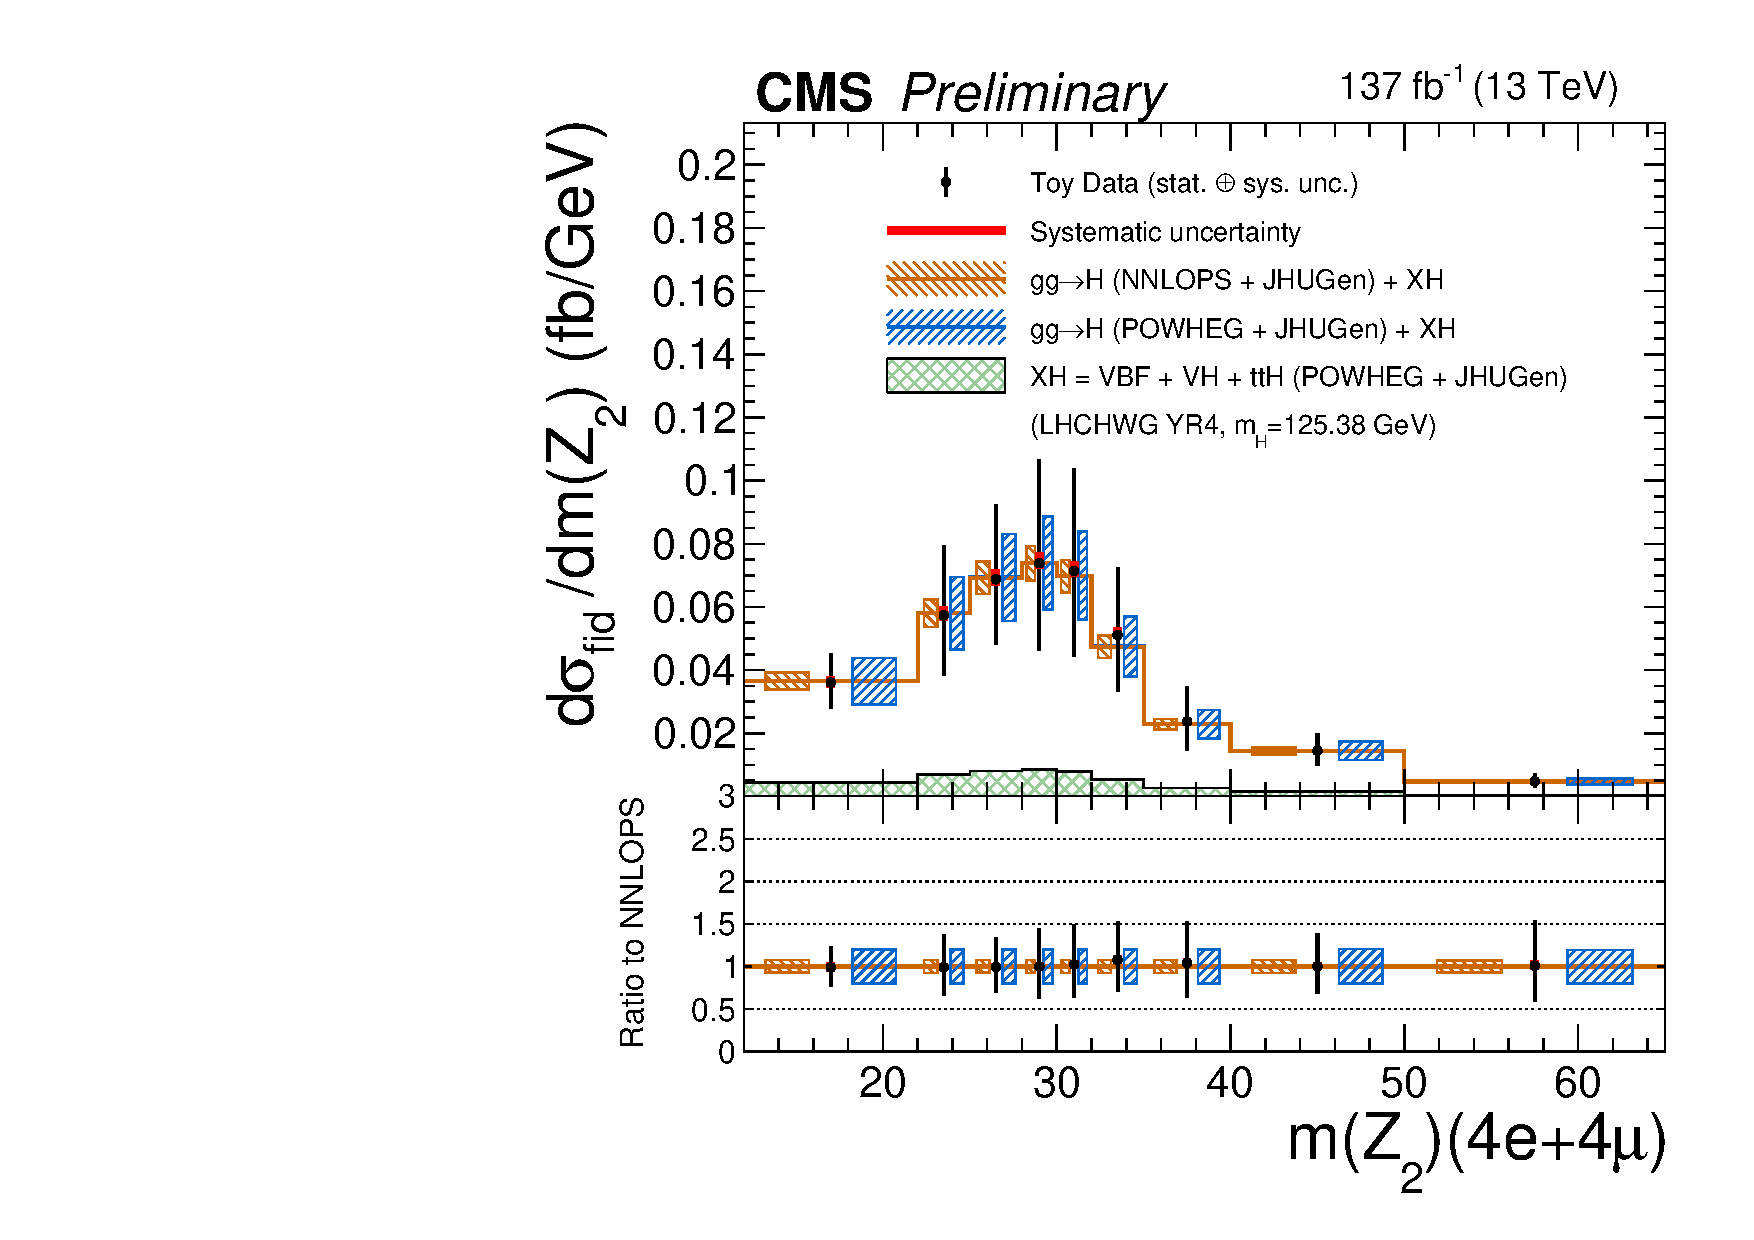
\includegraphics[width=0.48\textwidth]{Images/H4L/ZCands/model_v4/massZ2_unfoldwith_4l_SM_125_asimov.pdf}
		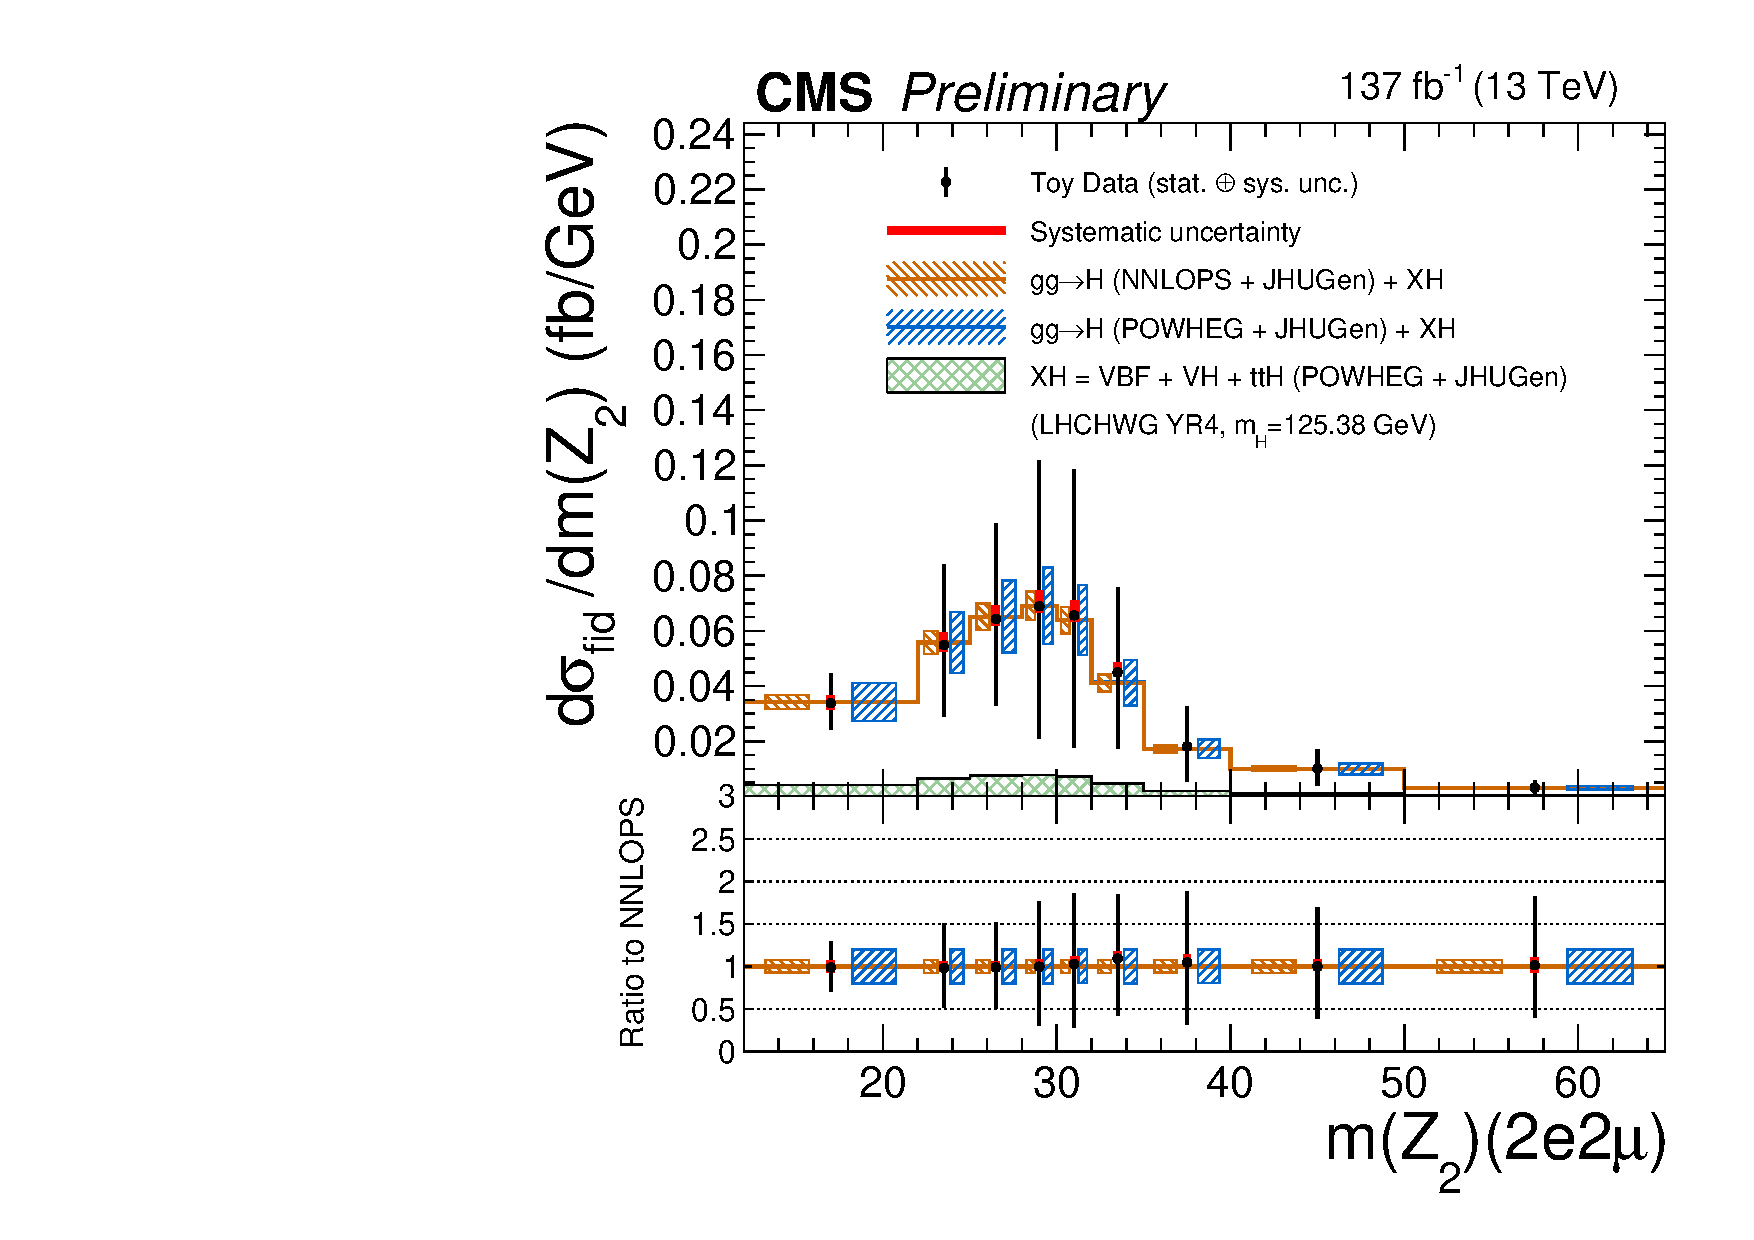
\includegraphics[width=0.48\textwidth]{Images/H4L/ZCands/model_v4/massZ2_unfoldwith_2e2mu_SM_125_asimov.pdf}\\
		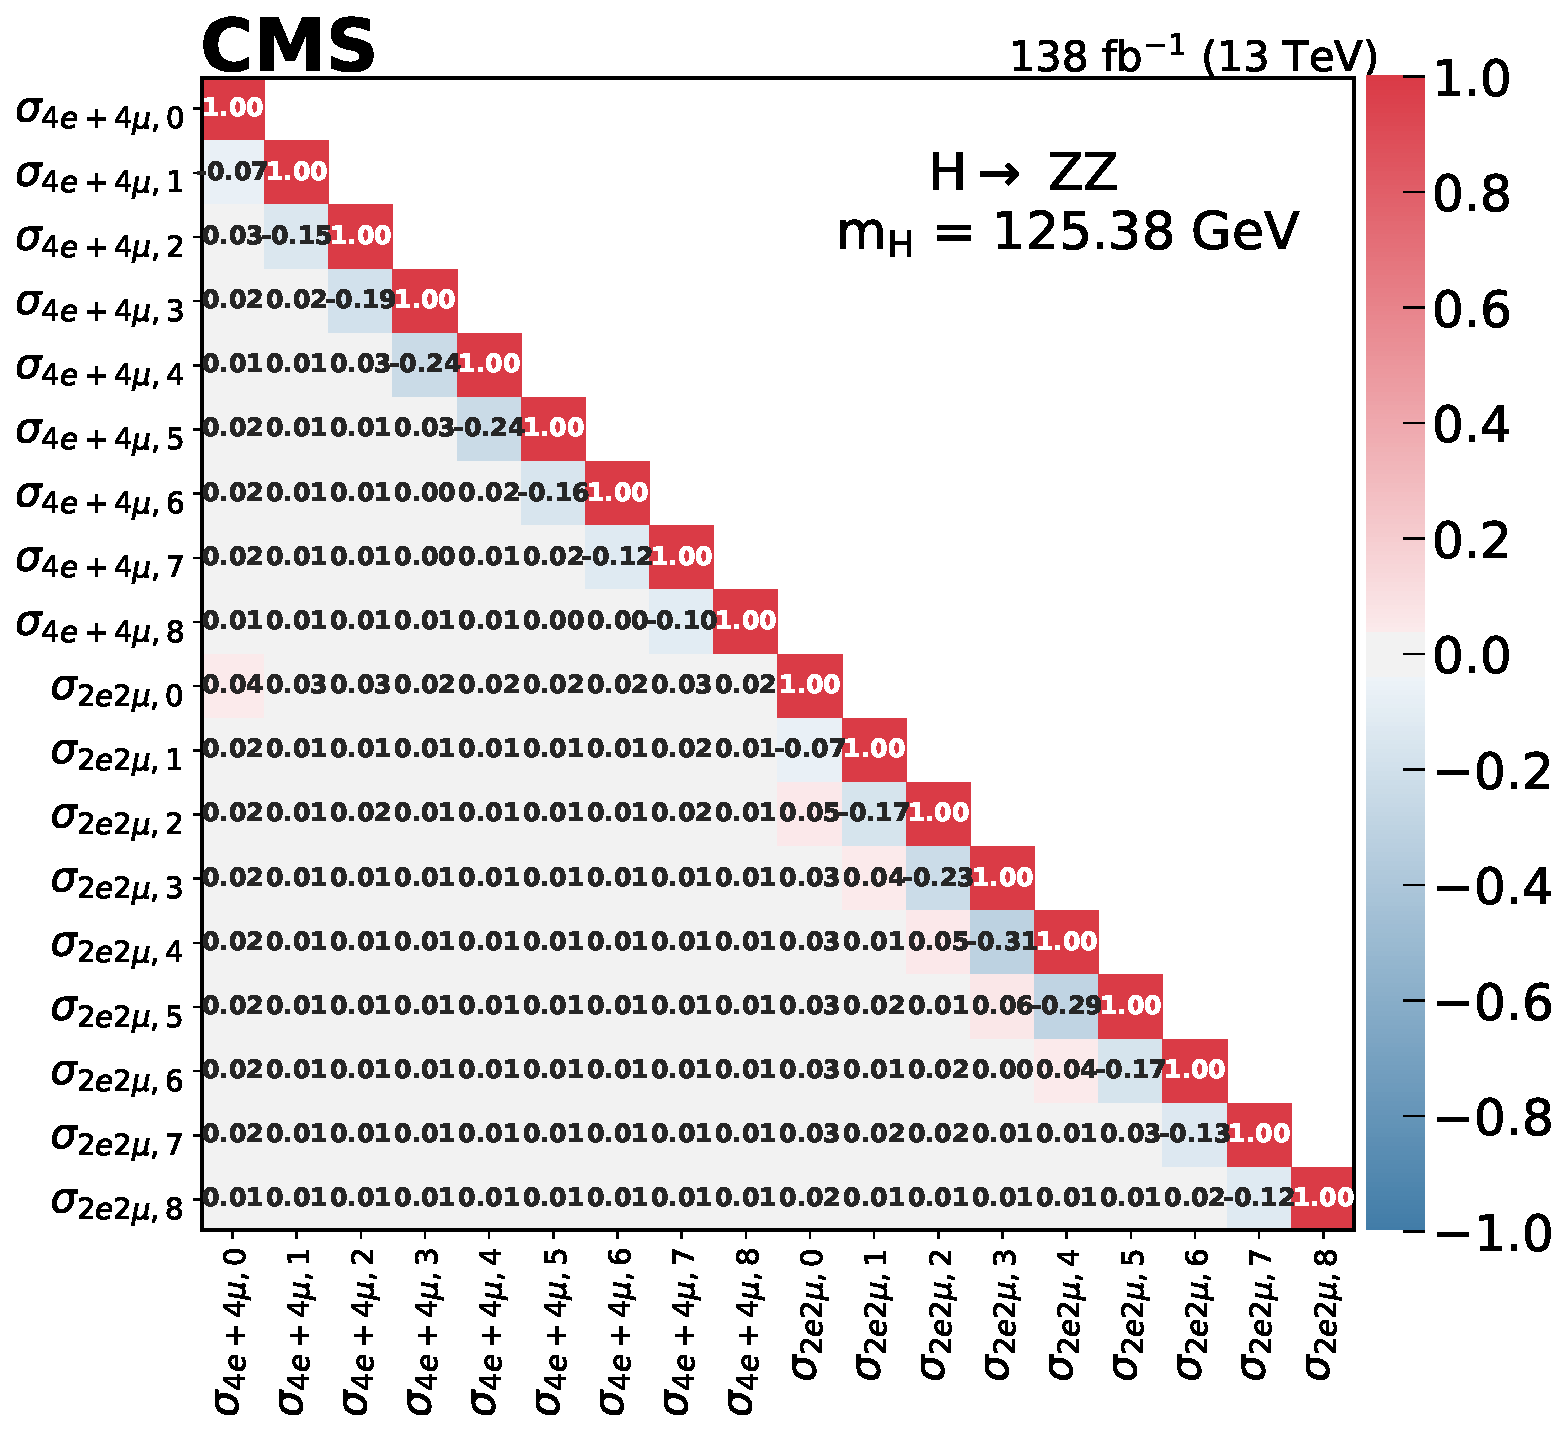
\includegraphics[width=0.48\textwidth]{Images/H4L/correlations/corr_massZ2_v4.pdf}\\	
		\caption{
			Differential cross sections as a function of the invariant mass of the sub-leading di-lepton pair $m_{\PZ_{2}}$ in the same-flavor (top left) and opposite-flavor (top right)  final states.
			The bottom plot shows the correlation matrix between the observed differential cross sections.
			The acceptance and theoretical uncertainties in the differential bins are calculated using the \POWHEG (blue), NNLOPS (orange), and MadGraph\_aMC@NLO (pink) generators.
			The sub-dominant component of the signal ($\VBF + \VH + \ttH$) is denoted as XH and it is fixed to the SM.
			\label{fig:fidMZ2}}
	\end{figure}
\end{center}

\clearpage

\begin{center}
	\begin{figure}[!htb]
		\centering
		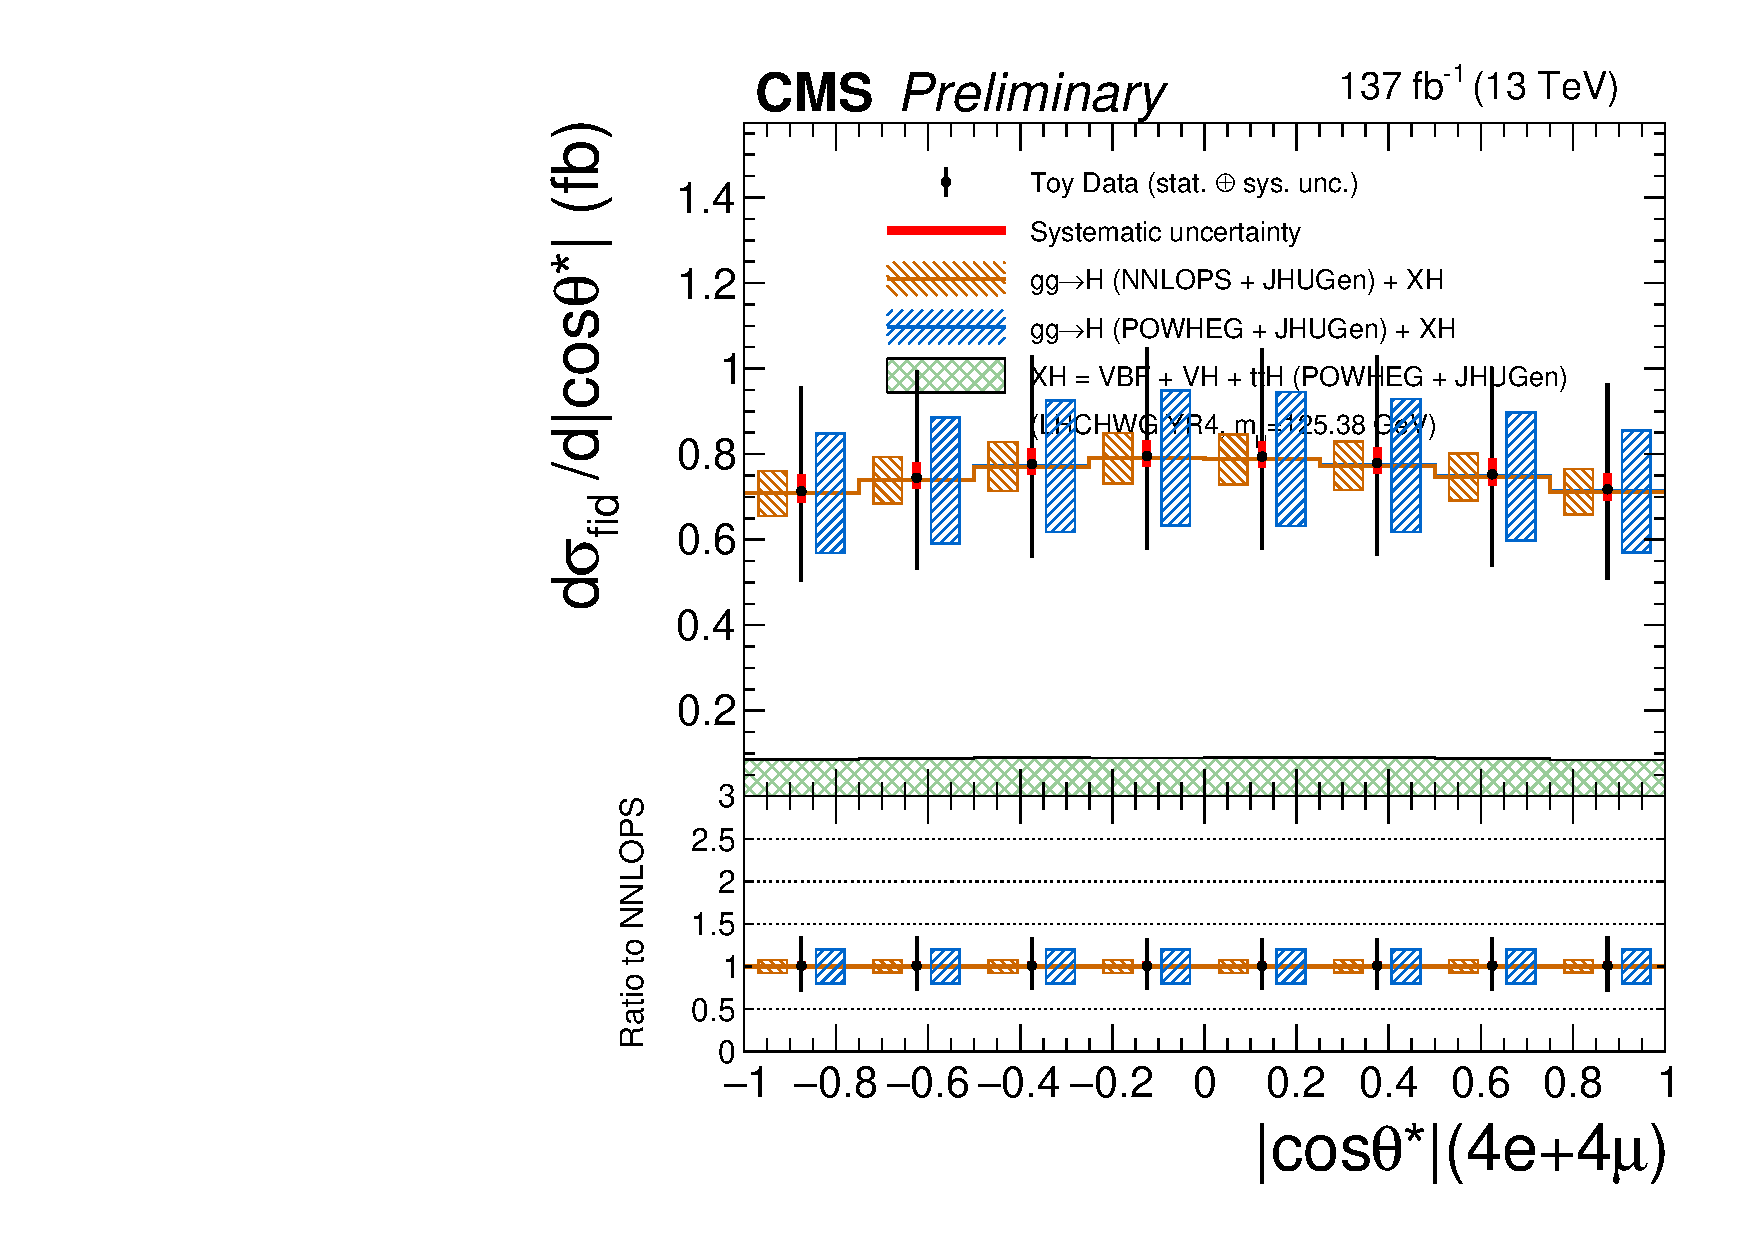
\includegraphics[width=0.48\textwidth]{Images/H4L/angles/model_v4/costhetastar_unfoldwith_4l_SM_125_asimov.pdf}
		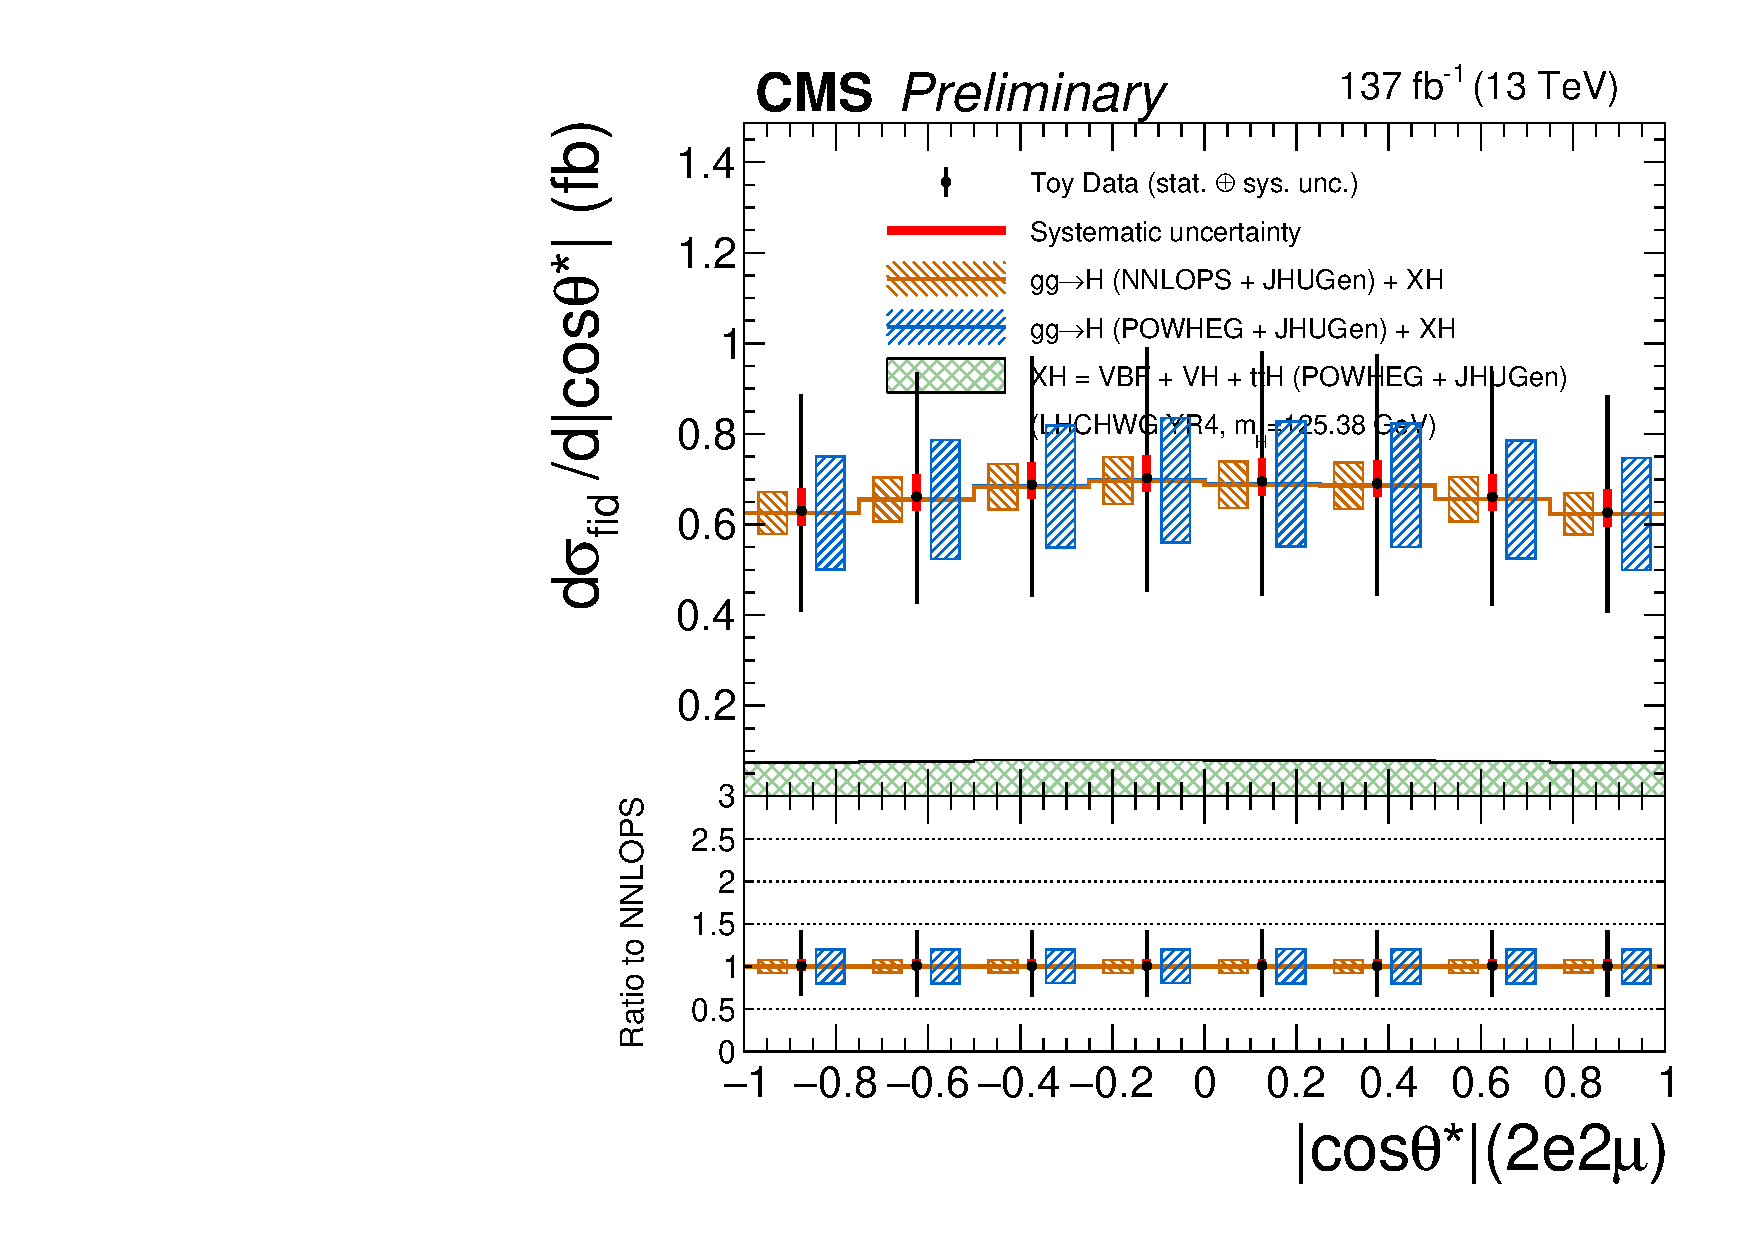
\includegraphics[width=0.48\textwidth]{Images/H4L/angles/model_v4/costhetastar_unfoldwith_2e2mu_SM_125_asimov.pdf} \\
		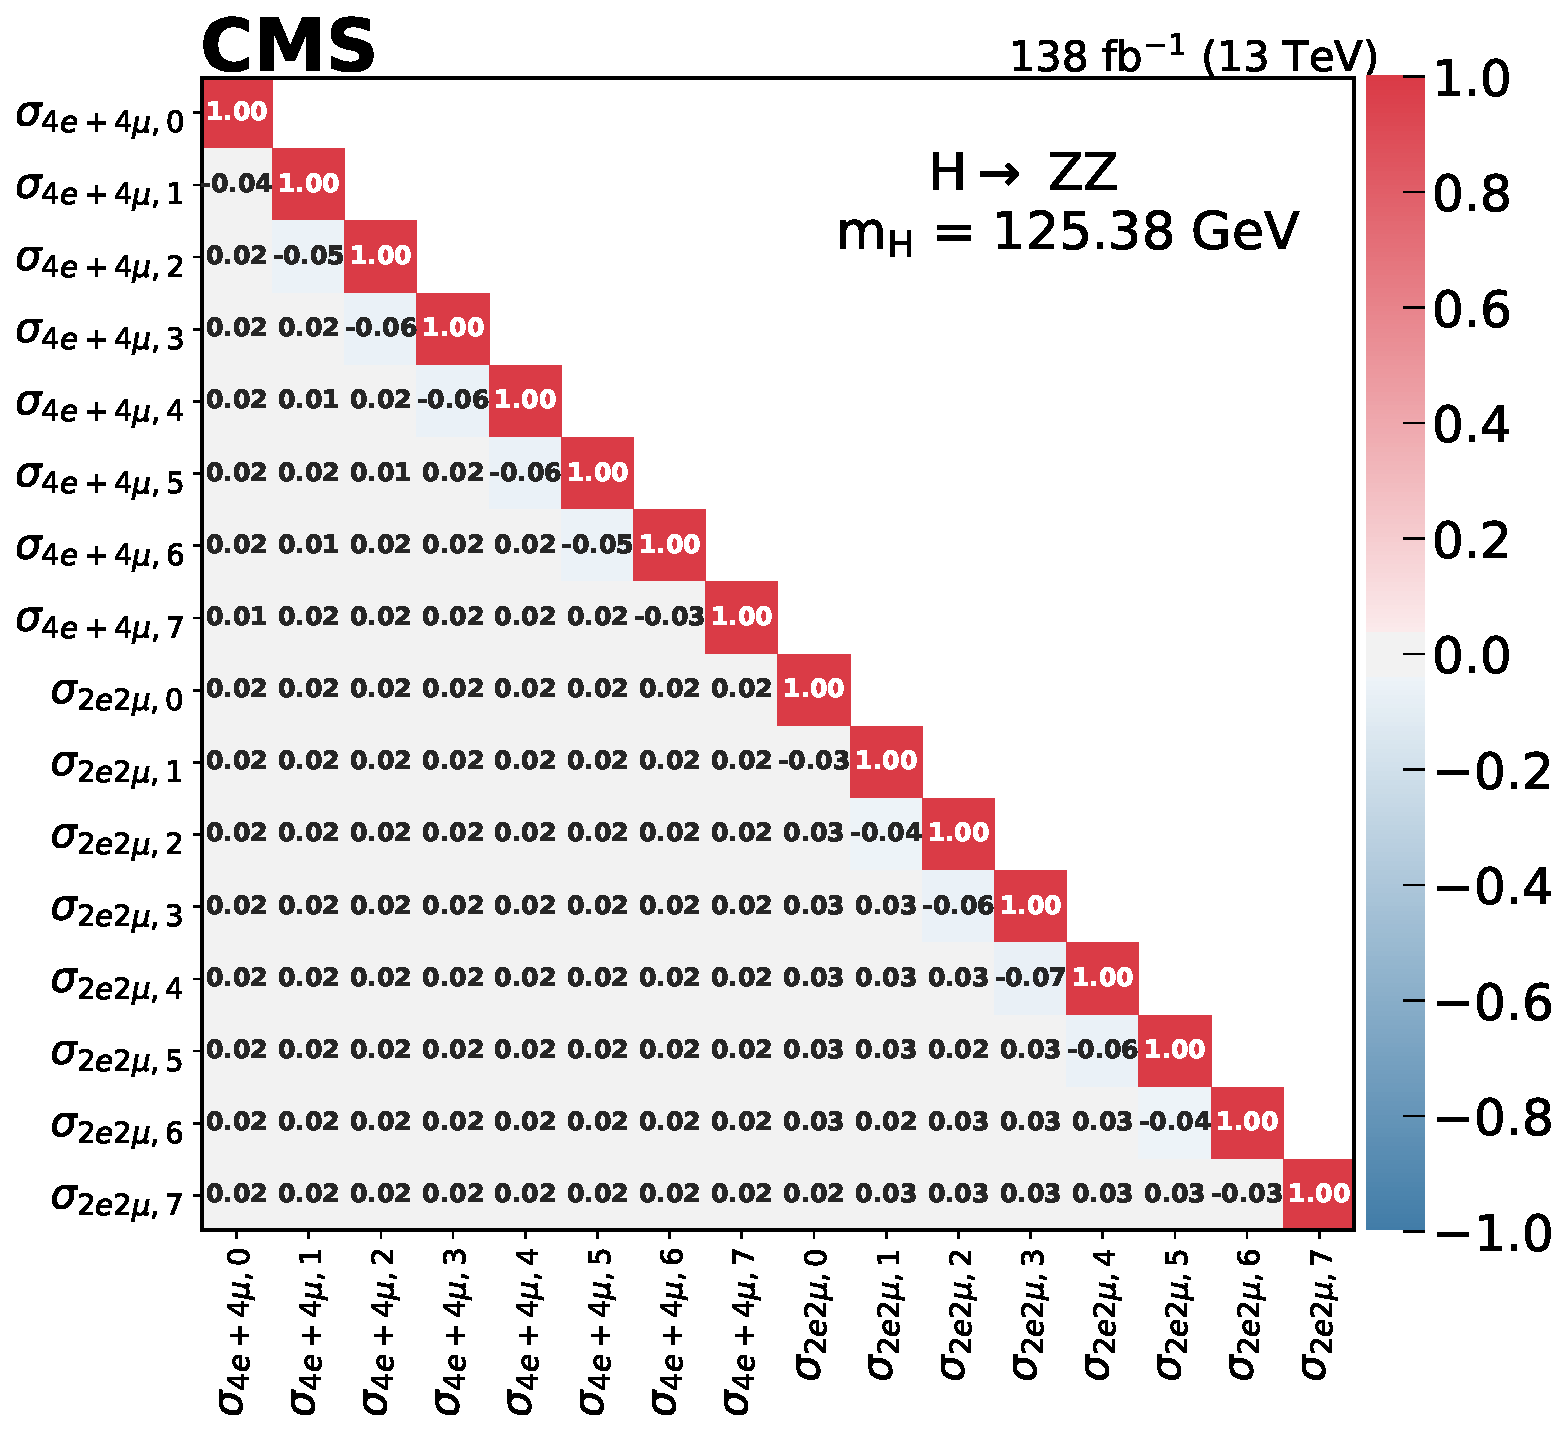
\includegraphics[width=0.48\textwidth]{Images/H4L/correlations/corr_costhetastar_v4.pdf} \\
		\caption{
			Differential cross sections as a function of  $\cos \theta^\star$ in the same-flavor (top left) and opposite-flavor (top right)  final states.
			The bottom plot shows the correlation matrix between the observed differential cross sections.
			The acceptance and theoretical uncertainties in the differential bins are calculated using the \POWHEG (blue), NNLOPS (orange), and MadGraph\_aMC@NLO (pink) generators.
			The sub-dominant component of the signal ($\VBF + \VH + \ttH$) is denoted as XH and it is fixed to the SM.
			\label{fig:fidCOSTS}}
	\end{figure}
\end{center}

\clearpage

\begin{center}
	\begin{figure}[!htb]
		\centering
		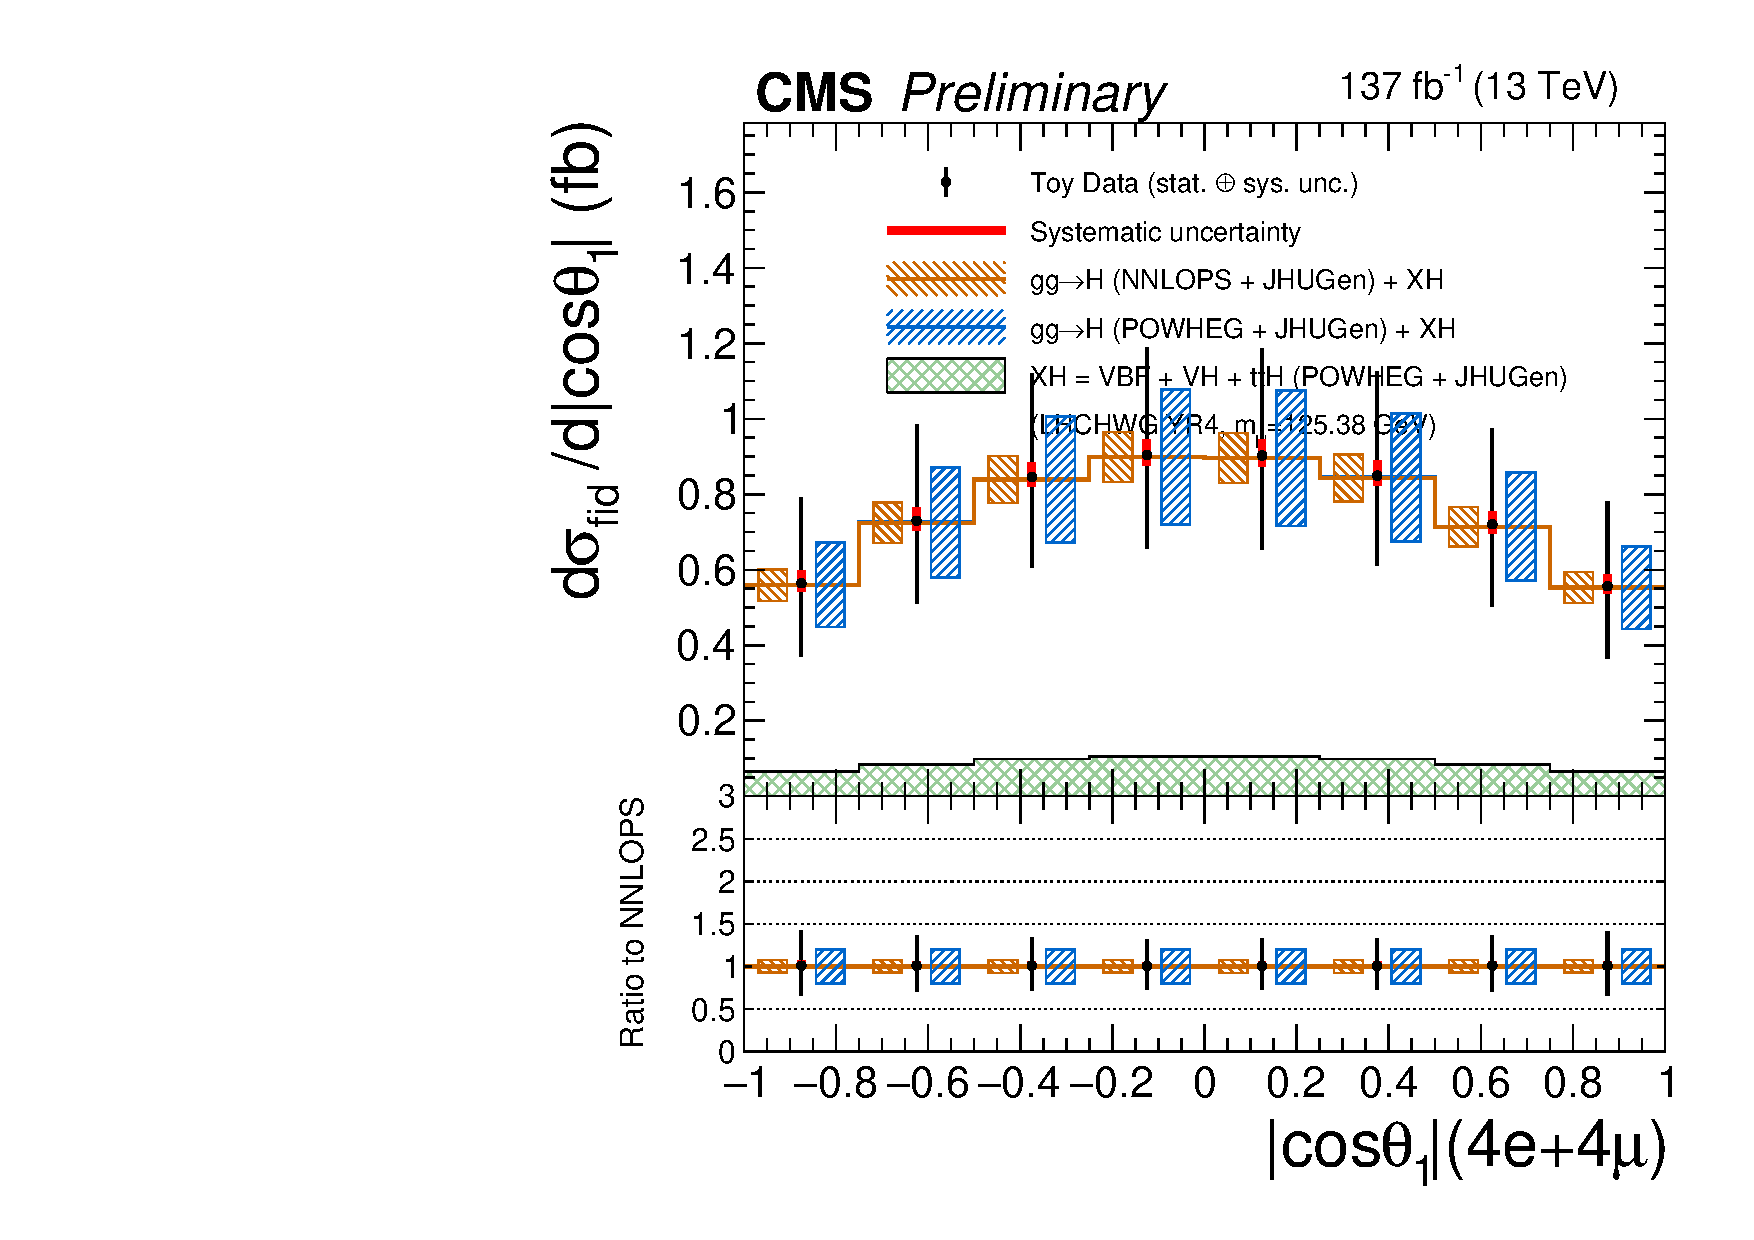
\includegraphics[width=0.48\textwidth]{Images/H4L/angles/model_v4/costhetaZ1_unfoldwith_4l_SM_125_asimov.pdf}
		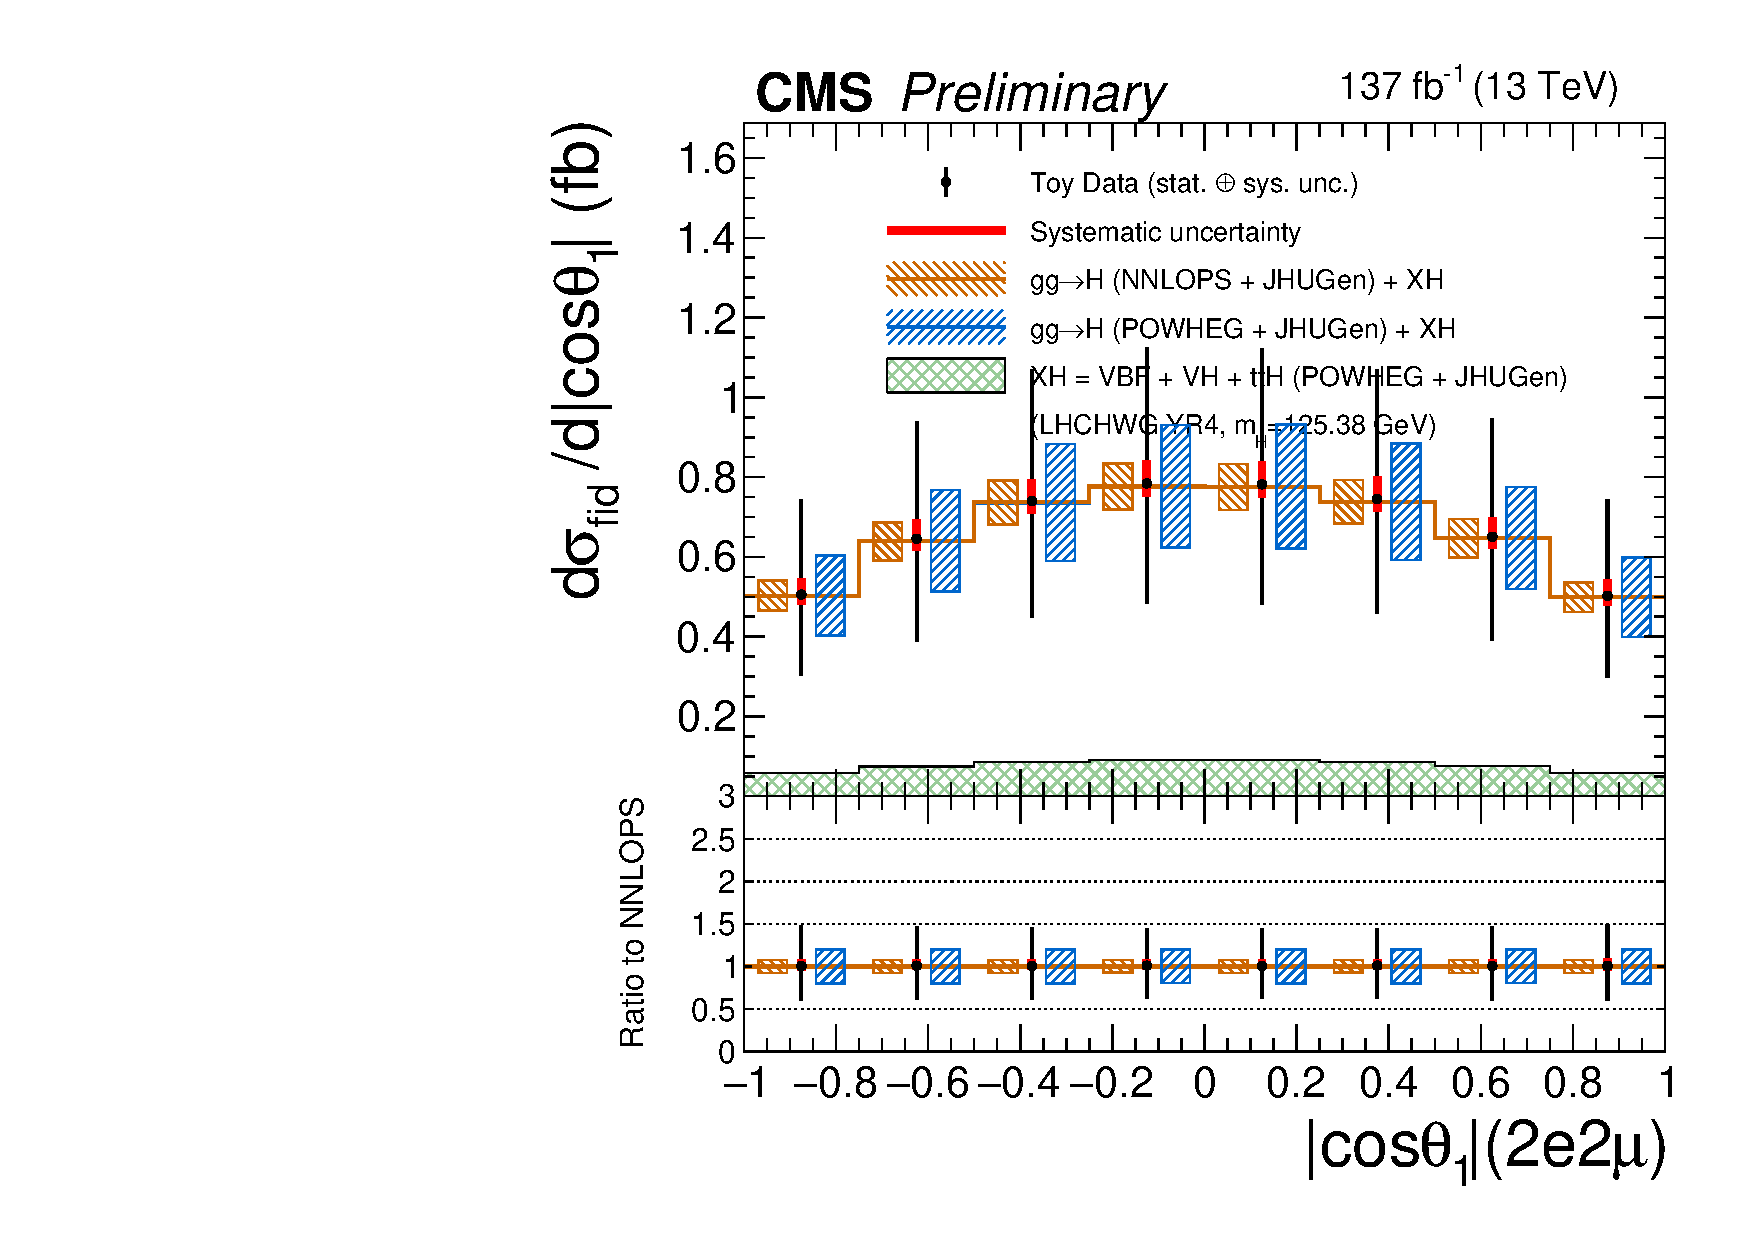
\includegraphics[width=0.48\textwidth]{Images/H4L/angles/model_v4/costhetaZ1_unfoldwith_2e2mu_SM_125_asimov.pdf} \\
		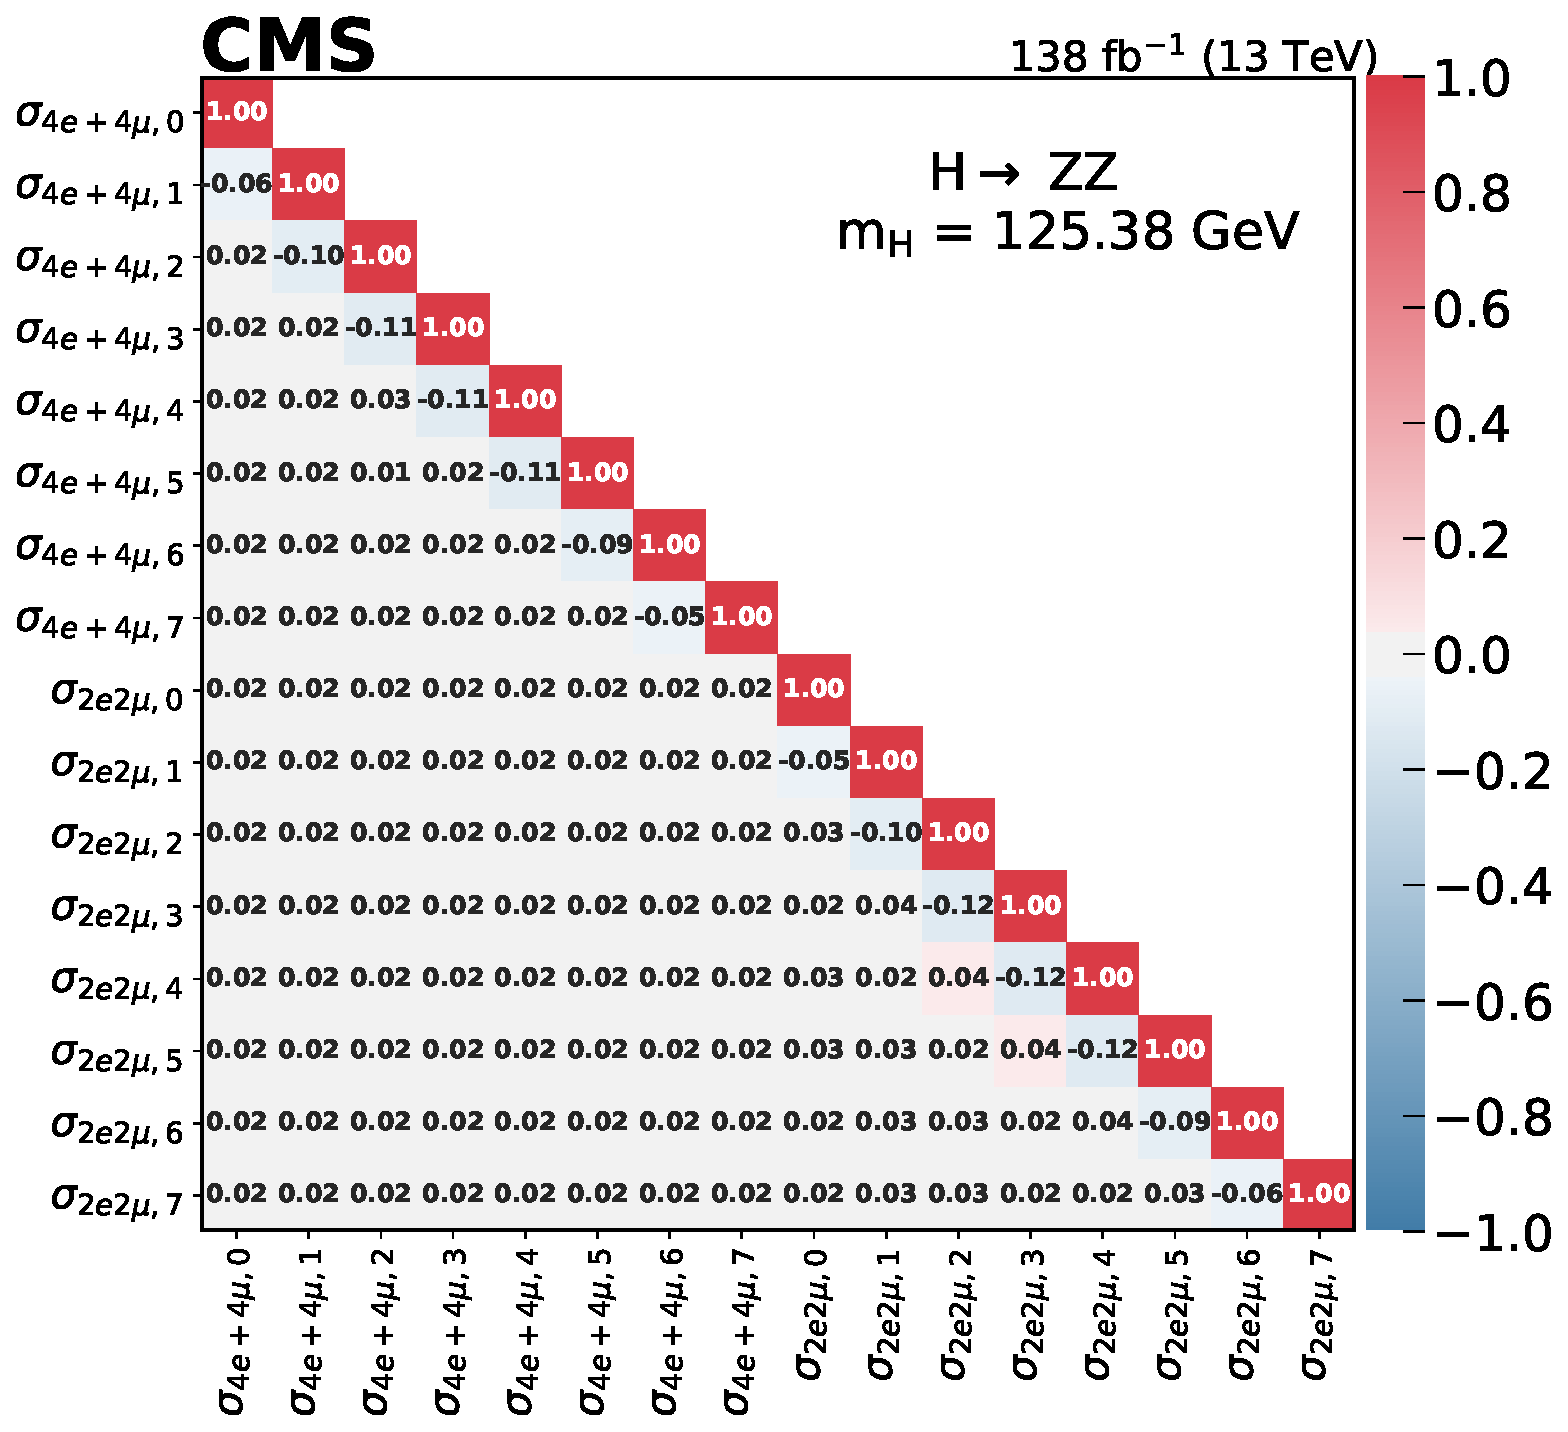
\includegraphics[width=0.48\textwidth]{Images/H4L/correlations/corr_costhetaZ1_v4.pdf} \\
		\caption{
			Differential cross sections as a function of $\cos \theta_\text{1}$ in the same-flavor (top left) and opposite-flavor (top right)  final states.
			The bottom plot shows the correlation matrix between the observed differential cross sections.
			The acceptance and theoretical uncertainties in the differential bins are calculated using the \POWHEG (blue), NNLOPS (orange), and MadGraph\_aMC@NLO (pink) generators.
			The sub-dominant component of the signal ($\VBF + \VH + \ttH$) is denoted as XH and it is fixed to the SM.
			\label{fig:fidCOSZ1}}
	\end{figure}
\end{center}

\clearpage

\begin{center}
	\begin{figure}[!htb]
		\centering
		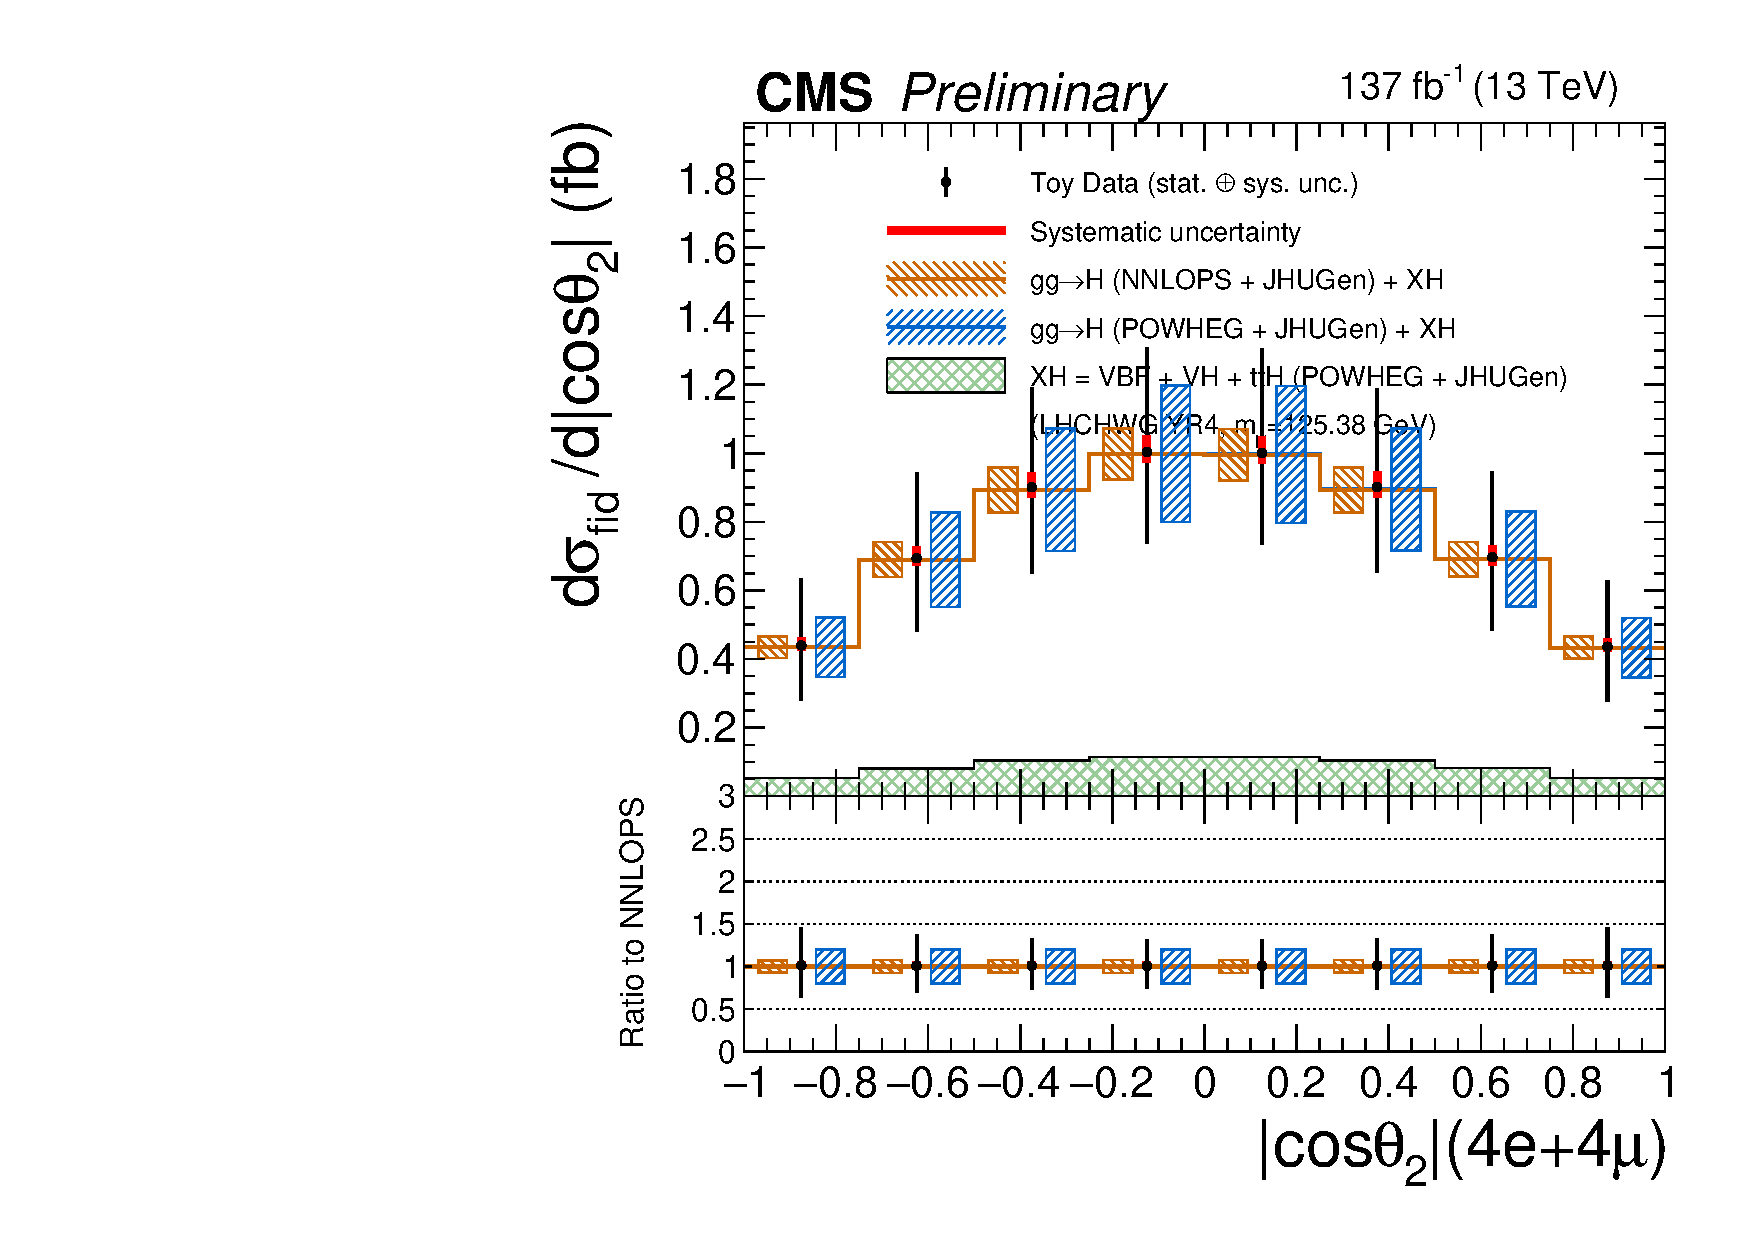
\includegraphics[width=0.48\textwidth]{Images/H4L/angles/model_v4/costhetaZ2_unfoldwith_4l_SM_125_asimov.pdf}
		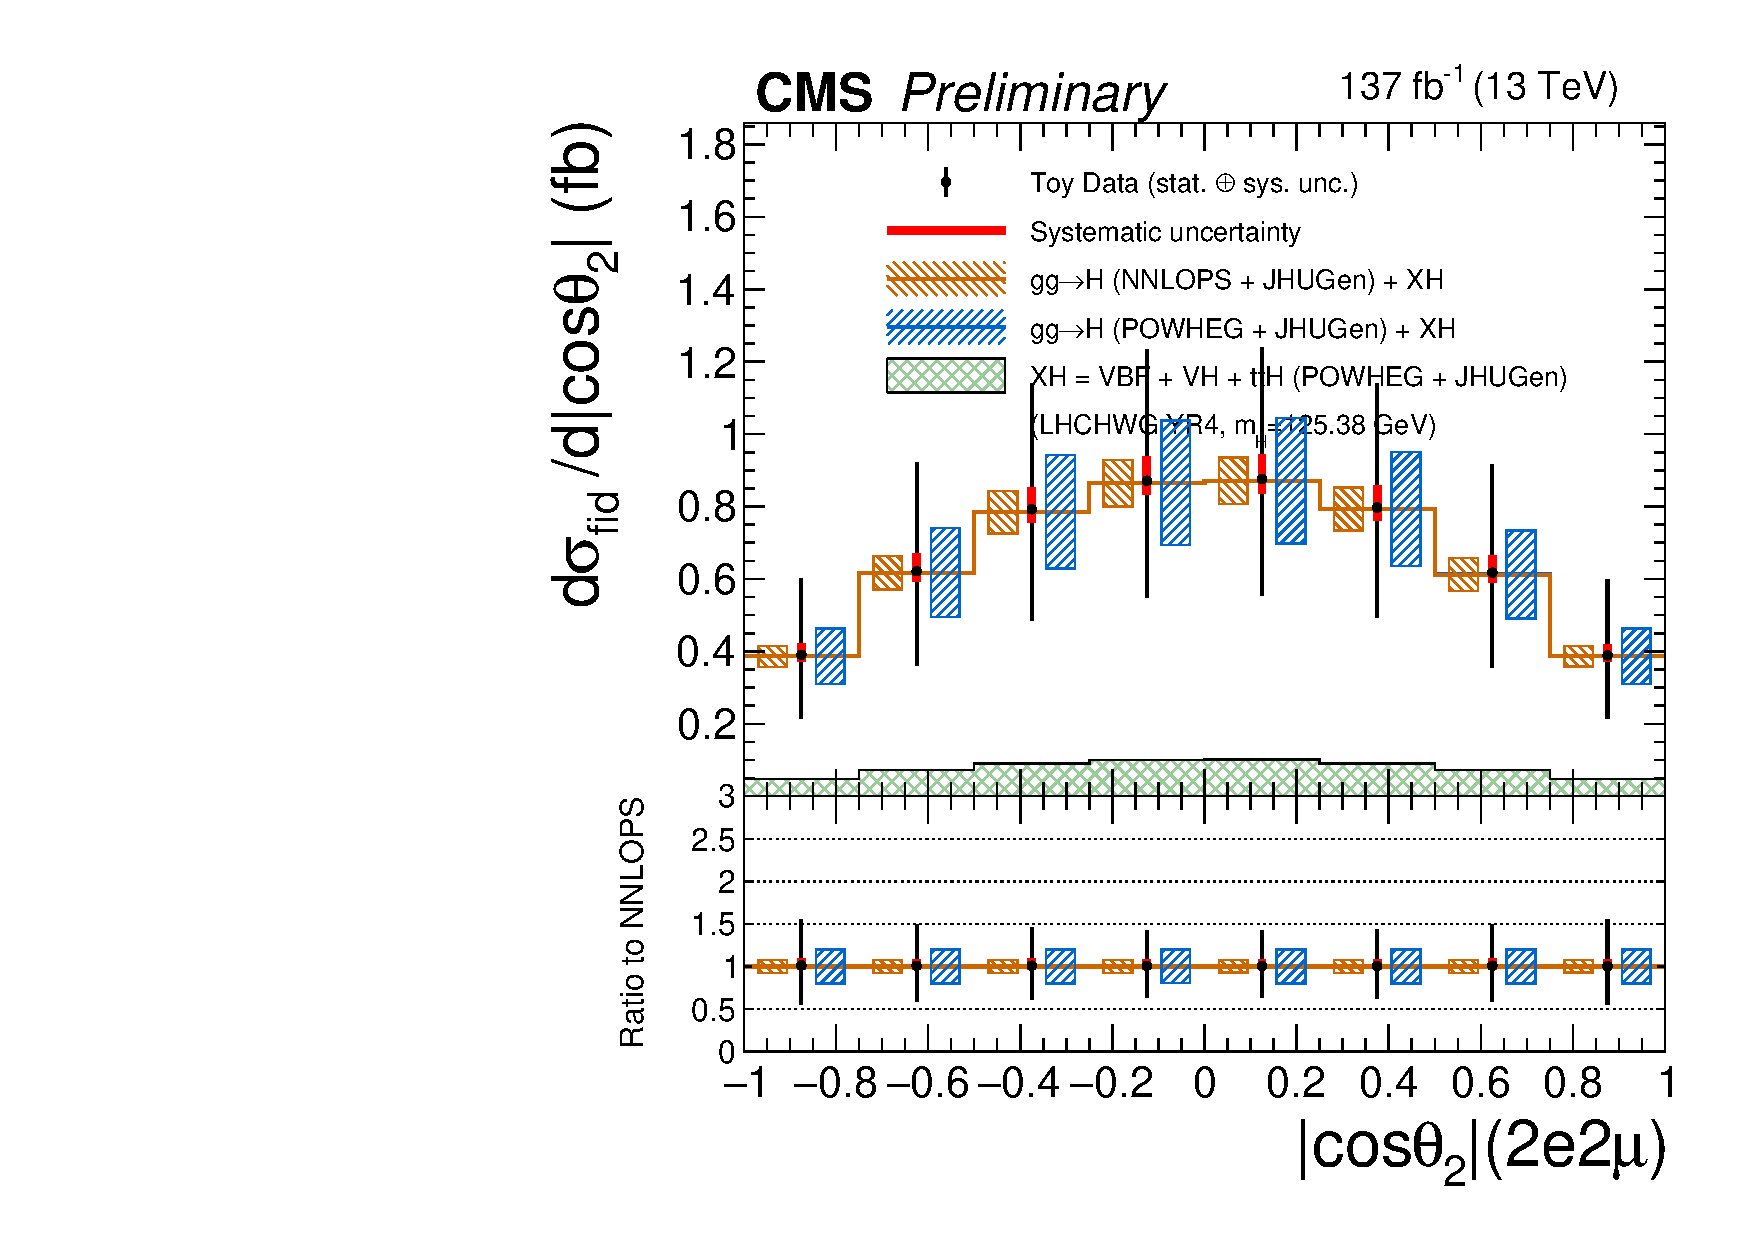
\includegraphics[width=0.48\textwidth]{Images/H4L/angles/model_v4/costhetaZ2_unfoldwith_2e2mu_SM_125_asimov.pdf} \\
		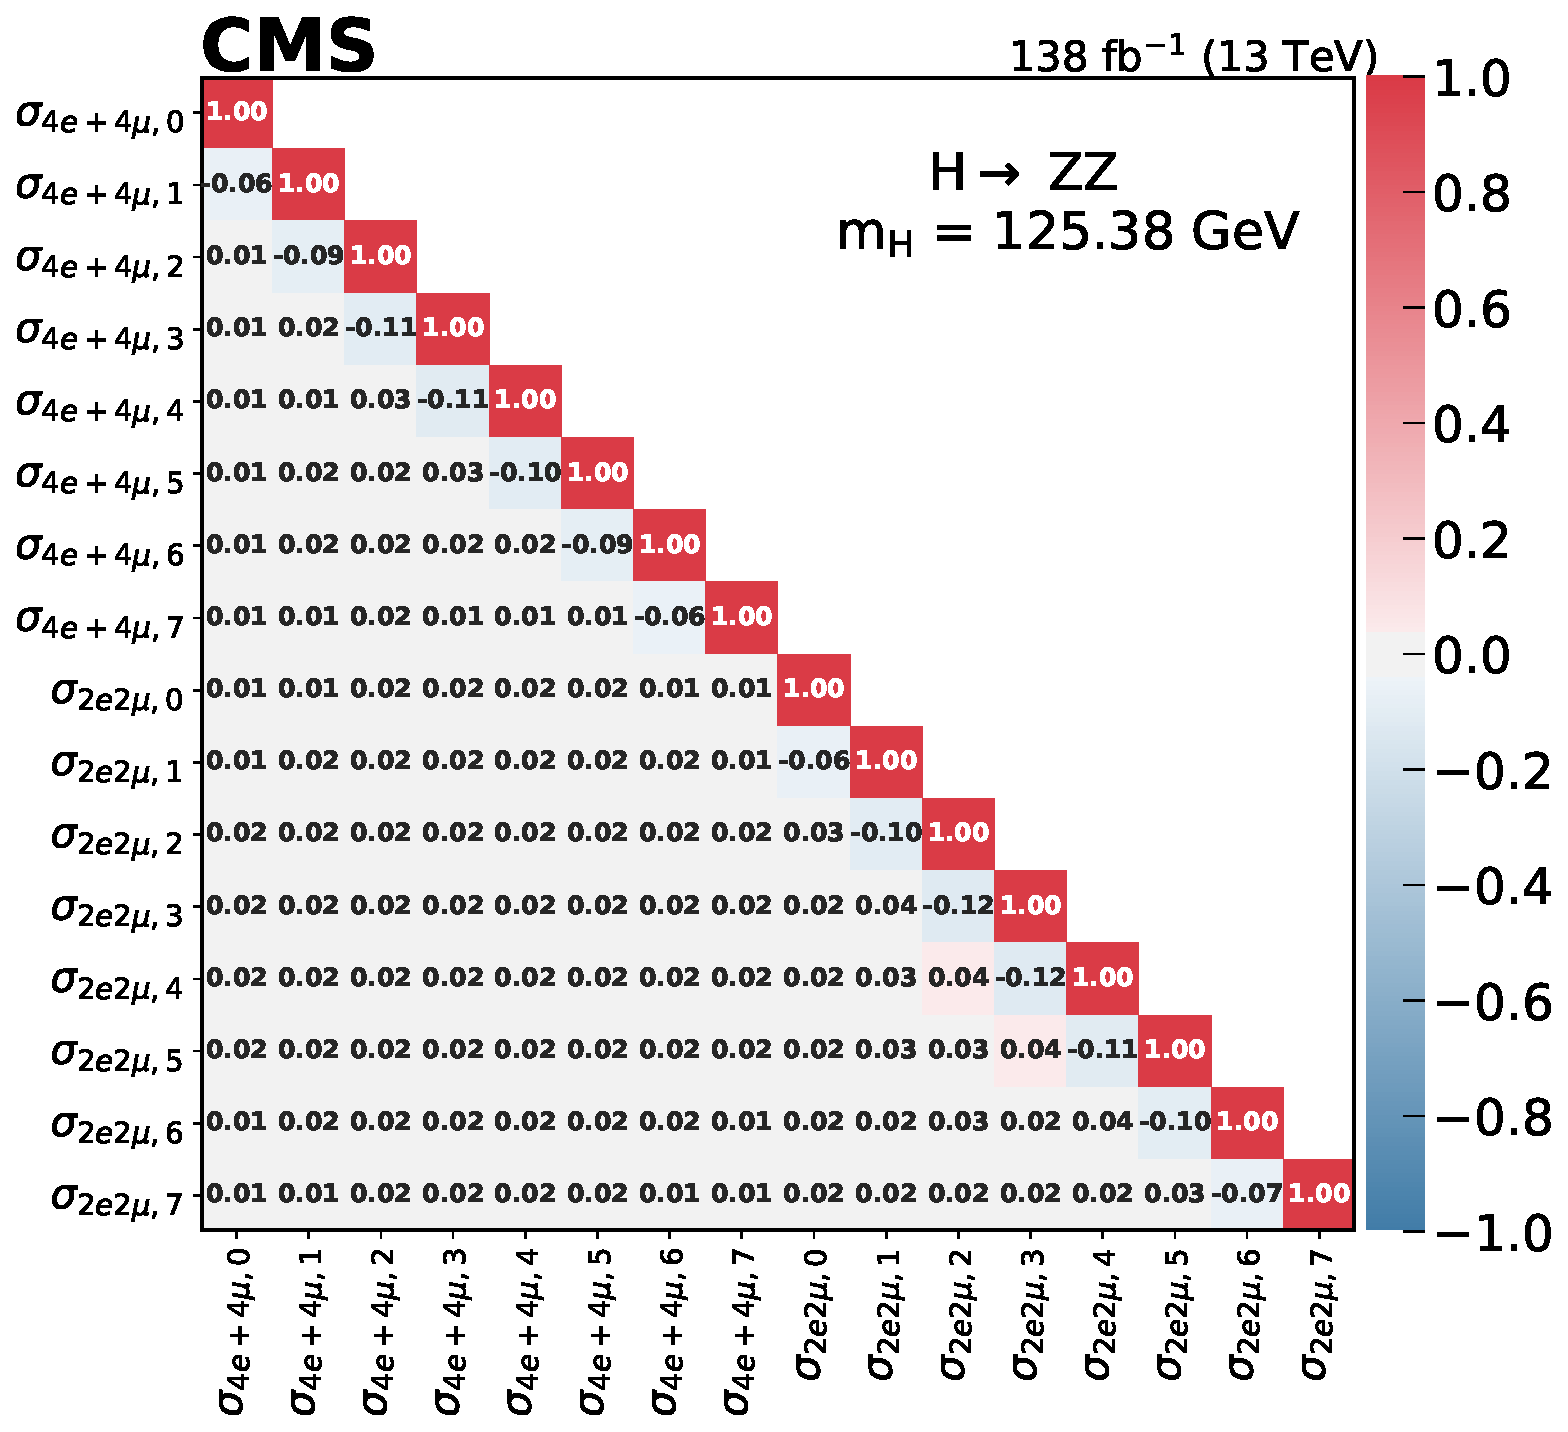
\includegraphics[width=0.48\textwidth]{Images/H4L/correlations/corr_costhetaZ2_v4.pdf} \\
		\caption{
			Differential cross sections as a function of  $\cos \theta_\text{2}$ in the same-flavor (top left) and opposite-flavor (top right)  final states.
			The bottom plot shows the correlation matrix between the observed differential cross sections.
			The acceptance and theoretical uncertainties in the differential bins are calculated using the \POWHEG (blue), NNLOPS (orange), and MadGraph\_aMC@NLO (pink) generators.
			The sub-dominant component of the signal ($\VBF + \VH + \ttH$) is denoted as XH and it is fixed to the SM.
			\label{fig:fidCOSZ2}}
	\end{figure}
\end{center}

\clearpage

\begin{center}
	\begin{figure}[!htb]
		\centering
		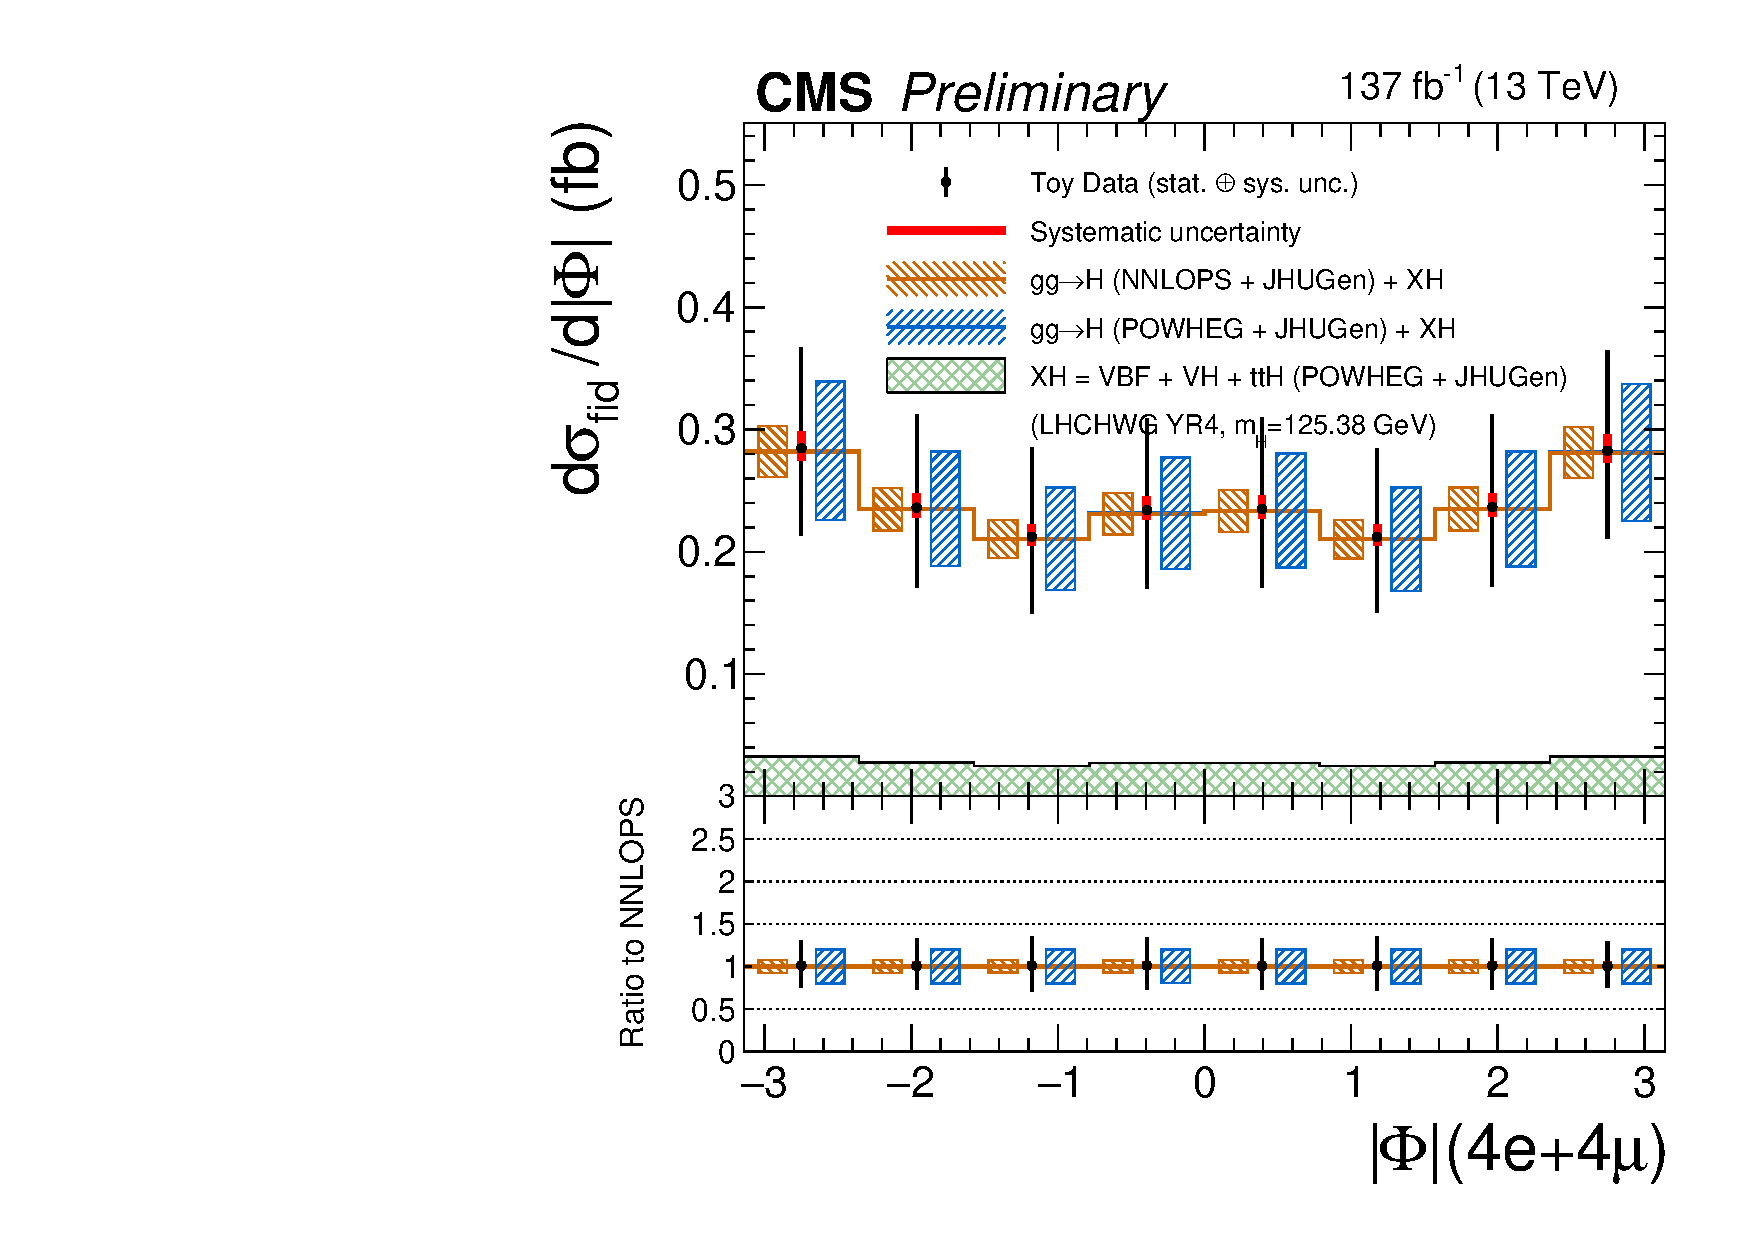
\includegraphics[width=0.48\textwidth]{Images/H4L/angles/model_v4/phi_unfoldwith_4l_SM_125_asimov.pdf}
		\includegraphics[width=0.48\textwidth]{Images/H4L/angles/model_v4/phi_unfoldwith_2e2mu_SM_125_asimov.pdf}\\
		\includegraphics[width=0.48\textwidth]{Images/H4L/correlations/corr_phi_v4.pdf} \\
		\caption{
			Differential cross sections as a function of the angle $\Phi$ in the same-flavor (top left) and opposite-flavor (top right)  final states.
			The bottom plot shows the correlation matrix between the observed differential cross sections.
			The acceptance and theoretical uncertainties in the differential bins are calculated using the \POWHEG (blue), NNLOPS (orange), and MadGraph\_aMC@NLO (pink) generators.
			The sub-dominant component of the signal ($\VBF + \VH + \ttH$) is denoted as XH and it is fixed to the SM.
			\label{fig:fidPHI}}
	\end{figure}
\end{center}

\clearpage

\begin{center}
	\begin{figure}[!htb]
		\centering
		\includegraphics[width=0.48\textwidth]{Images/H4L/angles/model_v4/phistar_unfoldwith_4l_SM_125_asimov.pdf}
		\includegraphics[width=0.48\textwidth]{Images/H4L/angles/model_v4/phistar_unfoldwith_2e2mu_SM_125_asimov.pdf}\\
		\includegraphics[width=0.48\textwidth]{Images/H4L/correlations/corr_phistar_v4.pdf} \\
		\caption{
			Differential cross sections as a function of the angle $\Phi_\text{1}$ in the same-flavor (top left) and opposite-flavor (top right)  final states.
			The bottom plot shows the correlation matrix between the observed differential cross sections.
			The acceptance and theoretical uncertainties in the differential bins are calculated using the \POWHEG (blue), NNLOPS (orange), and MadGraph\_aMC@NLO (pink) generators.
			The sub-dominant component of the signal ($\VBF + \VH + \ttH$) is denoted as XH and it is fixed to the SM.
			\label{fig:fidPHISTAR}}
	\end{figure}
\end{center}

\clearpage

%\subsection{Matrix element discriminants}
%The $\Pp\Pp\to\Hllll$ fiducial cross section is measured in bins of matrix element discriminants and the results are compared both with the SM predictions and the BSM distributions obtained for significative BSM scenarios, corresponding to the introduction of anomalous HVV couplings in the SM Lagrangian:
%\begin{widetext}
%	\begin{align}
	%	A(\PH\PV_1\PV_2) =
	%	\frac{1}{v}
	%	\left[ a_{1}^{\PV\PV}
	%	+ \frac{\kappa_1^{\PV\PV}q_{\PV1}^2 + \kappa_2^{\PV\PV} q_{\PV2}^{2}}{\left(\Lambda_{1}^{\PV\PV} \right)^{2}} 
	%	+ \frac{\kappa_3^{\PV\PV}(q_{\PV1} + q_{\PV2})^{2}}{\left(\Lambda_{Q}^{\PV\PV} \right)^{2}} \right]
	%	m_{\PV1}^2 \epsilon_{\PV1}^* \epsilon_{\PV2}^*  
	%	\nonumber \\
	%	+ \frac{1}{v}a_{2}^{\PV\PV}  f_{\mu \nu}^{*(1)}f^{*(2),\mu\nu}
	%	+ \frac{1}{v}a_{3}^{\PV\PV}   f^{*(1)}_{\mu \nu} {\tilde f}^{*(2),\mu\nu} ,
	%	\label{eq:formfact-fullampl-spin0}
	%	\end{align}
%\end{widetext}
%where $f^{(i){\mu \nu}} = \epsilon_{{\PV}i}^{\mu}q_{{\PV}i}^{\nu} - \epsilon_{{\PV}i}^\nu q_{{\PV}i}^{\mu}$,
%${\tilde f}^{(i)}_{\mu \nu} = \frac{1}{2} \epsilon_{\mu\nu\rho\sigma} f^{(i),\rho\sigma}$, and
%$\epsilon_{{\PV}i}$, $q_{{\PV}i}$, and $m_{{\PV}i}$ are the polarization vector, four-momentum, and pole mass 
%of a gauge boson $i=1$ or 2. The constants $\Lambda_{1}$ and $\Lambda_{Q}$ are the scales 
%of BSM physics necessary to keep the $\kappa_i^{\PV\PV}$ couplings unitless, 
%and $a_1^{\PV\PV}$, $a_2^{\PV\PV}$, $a_3^{\PV\PV}$, $\kappa_1^{\PV\PV}$, $\kappa_2^{\PV\PV}$, and $\kappa_3^{\PV\PV}$ 
%are real numbers that modify the corresponding amplitude terms.

%The fiducial differential cross sections measured are shown in Figure \ref{fig:fiducial_diff_Dzm}, where the results are compared with the SM prediction for the inclusive $\Pp\Pp\to\Hllll$ cross section and the corresponding distribution obtained for the introduction of HVV anomalous coupling in the decay.

%		Differential cross sections as a function of $\Dzm$ (top left), $\Dzhp$ (top right), and $\DCP$ (bottom).


\begin{center}%%%%%%%%%%%%%%%%%%%%%%%% Discriminants %%%%%%%%%%%%%%%%%%%%%%%%%
	\begin{figure}[!htb]
		\centering
		\includegraphics[width=0.48\textwidth]{Images/H4L/discriminants/model_v4/D0m_unfoldwith_4l_SM_125_asimov.pdf}
		\includegraphics[width=0.48\textwidth]{Images/H4L/discriminants/model_v4/D0m_unfoldwith_2e2mu_SM_125_asimov.pdf}\\
		\includegraphics[width=0.48\textwidth]{Images/H4L/correlations/corr_D0m_v4.pdf}\\
		\caption{
			Differential cross sections as a function of the matrix element kinematic discriminant $\Dzm$ in the same-flavor (top left) and opposite-flavor (top right)  final states.
			The bottom plot shows the correlation matrix between the observed differential cross sections.
			The acceptance and theoretical uncertainties in the differential bins are calculated using the \POWHEG (blue) generator.
			The HVV anomalous coupling distributions, labelled as AC, are computed with $f_{a3} = 1$, $f_{a2} = 1$, and $f_{a3} = 0.5$, respectively.
			\label{fig:fidDZM}}
	\end{figure}
\end{center}

\clearpage

\begin{center}
	\begin{figure}[!htb]
		\centering
		\includegraphics[width=0.48\textwidth]{Images/H4L/discriminants/model_v4/D0hp_unfoldwith_4l_SM_125_asimov.pdf}
		\includegraphics[width=0.48\textwidth]{Images/H4L/discriminants/model_v4/D0hp_unfoldwith_2e2mu_SM_125_asimov.pdf}\\
		\includegraphics[width=0.48\textwidth]{Images/H4L/correlations/corr_D0hp_v4.pdf}\\
		\caption{
			Differential cross sections as a function of the matrix element kinematic discriminant $\Dzhp$ in the same-flavor (top left) and opposite-flavor (top right)  final states.
			The bottom plot shows the correlation matrix between the observed differential cross sections.
			The acceptance and theoretical uncertainties in the differential bins are calculated using the \POWHEG (blue) generator.
			The HVV anomalous coupling distributions, labelled as AC, are computed with $f_{a3} = 1$, $f_{a2} = 1$, and $f_{a3} = 0.5$, respectively.
			\label{fig:fidDOHP}}
	\end{figure}
\end{center}

\clearpage

\begin{center}
	\begin{figure}[!htb]
		\centering
		\includegraphics[width=0.48\textwidth]{Images/H4L/discriminants/model_v4/Dcp_unfoldwith_4l_SM_125_asimov.pdf}
		\includegraphics[width=0.48\textwidth]{Images/H4L/discriminants/model_v4/Dcp_unfoldwith_2e2mu_SM_125_asimov.pdf}\\
		\includegraphics[width=0.48\textwidth]{Images/H4L/correlations/corr_Dcp_v4.pdf}\\
		\caption{
			Differential cross sections as a function of the matrix element kinematic discriminant $\DCP$ in the same-flavor (top left) and opposite-flavor (top right)  final states.
			The bottom plot shows the correlation matrix between the observed differential cross sections.
			The acceptance and theoretical uncertainties in the differential bins are calculated using the \POWHEG (blue) generator.
			The HVV anomalous coupling distributions, labelled as AC, are computed with $f_{a3} = 1$, $f_{a2} = 1$, and $f_{a3} = 0.5$, respectively.
			\label{fig:fidDCP}}
	\end{figure}
\end{center}

\clearpage

\begin{center}
	\begin{figure}[!htb]
		\centering
		\includegraphics[width=0.48\textwidth]{Images/H4L/discriminants/model_v4/Dint_unfoldwith_4l_SM_125_asimov.pdf}
		\includegraphics[width=0.48\textwidth]{Images/H4L/discriminants/model_v4/Dint_unfoldwith_2e2mu_SM_125_asimov.pdf}\\
		\includegraphics[width=0.48\textwidth]{Images/H4L/correlations/corr_Dint_v4.pdf}\\
		\caption{
			Differential cross sections as a function of the matrix element kinematic discriminant $\Dint$ in the same-flavor (top left) and opposite-flavor (top right)  final states.
			The bottom plot shows the correlation matrix between the observed differential cross sections.
			The acceptance and theoretical uncertainties in the differential bins are calculated using the \POWHEG (blue) generator.
			The HVV anomalous coupling distributions, labelled as AC, are computed with $f_{a3} = 1$, $f_{a2} = 1$, and $f_{a3} = 0.5$, respectively.
			\label{fig:fidDINT}}
	\end{figure}
\end{center}

\clearpage

\begin{center}
	\begin{figure}[!htb]
		\centering
		\includegraphics[width=0.48\textwidth]{Images/H4L/discriminants/model_v4/DL1_unfoldwith_4l_SM_125_asimov.pdf}
		\includegraphics[width=0.48\textwidth]{Images/H4L/discriminants/model_v4/DL1_unfoldwith_2e2mu_SM_125_asimov.pdf}\\
		\includegraphics[width=0.48\textwidth]{Images/H4L/correlations/corr_DL1_v4.pdf}\\
		\caption{
			Differential cross sections as a function of the matrix element kinematic discriminant $\DLone$ in the same-flavor (top left) and opposite-flavor (top right)  final states.
			The bottom plot shows the correlation matrix between the observed differential cross sections.
			The acceptance and theoretical uncertainties in the differential bins are calculated using the \POWHEG (blue) generator.
			The HVV anomalous coupling distributions, labelled as AC, are computed with $f_{a3} = 1$, $f_{a2} = 1$, and $f_{a3} = 0.5$, respectively.
			\label{fig:fidDL1}}
	\end{figure}
\end{center}

\clearpage

\begin{center}
	\begin{figure}[!htb]
		\centering
		\includegraphics[width=0.48\textwidth]{Images/H4L/discriminants/model_v4/DL1Zg_unfoldwith_4l_SM_125_logscale_asimov.pdf}
		\includegraphics[width=0.48\textwidth]{Images/H4L/discriminants/model_v4/DL1Zg_unfoldwith_2e2mu_SM_125_logscale_asimov.pdf}\\
		\includegraphics[width=0.48\textwidth]{Images/H4L/correlations/corr_DL1Zg_v4.pdf}\\
		\caption{
			Differential cross sections as a function of the matrix element kinematic discriminant $\DLoneZg$ in the same-flavor (top left) and opposite-flavor (top right)  final states.
			The bottom plot shows the correlation matrix between the observed differential cross sections.
			The acceptance and theoretical uncertainties in the differential bins are calculated using the \POWHEG (blue) generator.
			The HVV anomalous coupling distributions, labelled as AC, are computed with $f_{a3} = 1$, $f_{a2} = 1$, and $f_{a3} = 0.5$, respectively.
			\label{fig:fidDL1ZG}}
	\end{figure}
\end{center}

\clearpage

\subsection{Double differential cross sections}
The differential cross section measurements presented so far ensure a good coverage of the production and decay phase sapces in the $\Hllll$ channel, together with a separation of possible interference effects present in the same and opposite flavour final states.
In order to ensure a complete characterisation of this decay channel and to have a maximal coverage and separation of the different phase space regions, a set of double-differential measurements is also performed.

Cross sections are measured in bins of $\abs{y^{\PH}}$ vs $\pt^{\PH}$ (Fig.~\ref{fig:fidYHPTH}), number of associated jets vs  $\pt^{\PH}$ (Fig.~\ref{fig:fidNJPTH}), $\pt^{\PH j}$ vs $\pt^{\PH}$ (Fig.~\ref{fig:fidPTHPTHJ}), $\mathcal{T}_{\text{C}}$ vs $\pt^{\PH}$ (Fig.~\ref{fig:fidTCPTH}), $m_{\PZ_{1}}$ vs $m_{\PZ_{2}}$ (Fig.~\ref{fig:fidMZ1MZ2}), and \pt of the leading  vs sub-leading jet (Fig.~\ref{fig:fidPTJ1PTJ2}).

\clearpage

%%%%%%%%%%%%%%%%%%%%%%%% Double diff pTH %%%%%%%%%%%%%%%%%%%%%%%%%

\begin{center}
	\begin{figure}[!htb]
		\centering
		\includegraphics[width=0.48\textwidth]{Images/H4L/doublediff/rapidity4l_pT4l_unfoldwith_SM_125_logscale_asimov.pdf}
		\includegraphics[width=0.48\textwidth]{Images/H4L/correlations/corr_rapidity4l_pT4l_v3.pdf}\\
		\caption{
			Double differential cross sections in bins of $\abs{y^{\PH}}$ vs $\pt^{\PH}$ (left) and the correlation matrix between the observed differential cross sections (right).
			The acceptance and theoretical uncertainties in the differential bins are calculated using the \POWHEG (blue), NNLOPS (orange), and MadGraph\_aMC@NLO (pink) generators.
			The sub-dominant component of the signal ($\VBF + \VH + \ttH$) is denoted as XH and it is fixed to the SM.
			\label{fig:fidYHPTH}}
	\end{figure}
\end{center}

\clearpage

\begin{center}
	\begin{figure}[!htb]
		\centering
		\includegraphics[width=0.48\textwidth]{Images/H4L/doublediff/plot_njets_pt30_eta2p5_pT4l.png}
% 		\includegraphics[width=0.48\textwidth]{example-image-a}\\
		\caption{
			Double differential cross sections in bins of the number of associated jets in the event vs $\pt^{\PH}$ (left) and the correlation matrix between the observed differential cross sections (right).
			The acceptance and theoretical uncertainties in the differential bins are calculated using the \POWHEG (blue), NNLOPS (orange), and MadGraph\_aMC@NLO (pink) generators.
			The sub-dominant component of the signal ($\VBF + \VH + \ttH$) is denoted as XH and it is fixed to the SM.
			\label{fig:fidNJPTH}}
	\end{figure}
\end{center}

\clearpage

\begin{center}
	\begin{figure}[!htb]
		\centering
		\includegraphics[width=0.48\textwidth]{Images/H4L/doublediff/pT4l_pTHj_unfoldwith_SM_125_logscale_asimov.pdf}
		\includegraphics[width=0.48\textwidth]{Images/H4L/correlations/corr_pT4l_pTHj_v3.pdf}\\
		\caption{
			Double differential cross sections in bins of $\pt^{\PH j}$ vs $\pt^{\PH}$  (left) and the correlation matrix between the observed differential cross sections (right).
			The acceptance and theoretical uncertainties in the differential bins are calculated using the \POWHEG (blue), NNLOPS (orange), and MadGraph\_aMC@NLO (pink) generators.
			The sub-dominant component of the signal ($\VBF + \VH + \ttH$) is denoted as XH and it is fixed to the SM.
			\label{fig:fidPTHPTHJ}}
	\end{figure}
\end{center}

\clearpage

\begin{center}
	\begin{figure}[!htb]
		\centering
		\includegraphics[width=0.48\textwidth]{Images/H4L/doublediff/TCjmax_pT4l_unfoldwith_SM_125_logscale_asimov.pdf}
		\includegraphics[width=0.48\textwidth]{Images/H4L/correlations/corr_TCjmax_pT4l_v3.pdf}\\
		\caption{
			Double differential cross sections in bins of $\mathcal{T}_{\text{C}}$ vs $\pt^{\PH}$ (left) and the correlation matrix between the observed differential cross sections (right).
			The acceptance and theoretical uncertainties in the differential bins are calculated using the \POWHEG (blue), NNLOPS (orange), and MadGraph\_aMC@NLO (pink) generators.
			The sub-dominant component of the signal ($\VBF + \VH + \ttH$) is denoted as XH and it is fixed to the SM.
			\label{fig:fidTCPTH}}
	\end{figure}
\end{center}

\clearpage

\begin{center}
	\begin{figure}[!htb]
		\centering
		\includegraphics[width=0.48\textwidth]{Images/H4L/doublediff/massZ1_massZ2_unfoldwith_SM_125_logscale_asimov.pdf}
		\includegraphics[width=0.48\textwidth]{Images/H4L/correlations/corr_massZ1_massZ2_v3.pdf}\\
		\caption{
			Double differential cross section as a function of $m_{\PZ_{1}}$ vs $m_{\PZ_{2}}$ (left) and the correlation matrix between the observed differential cross sections (right).
			The acceptance and theoretical uncertainties in the differential bins are calculated using the \POWHEG (blue), NNLOPS (orange), and MadGraph\_aMC@NLO (pink) generators.
			The sub-dominant component of the signal ($\VBF + \VH + \ttH$) is denoted as XH and it is fixed to the SM.
			\label{fig:fidMZ1MZ2}}
	\end{figure}
\end{center}

\clearpage

\begin{center}
	\begin{figure}[!htb]
		\centering
		\includegraphics[width=0.48\textwidth]{Images/H4L/doublediff/pTj1_pTj2_unfoldwith_SM_125_logscale_asimov.pdf}
		\includegraphics[width=0.48\textwidth]{Images/H4L/correlations/corr_pTj1_pTj2_v3.pdf}\\
		\caption{
			Double differential cross section as a function of \pt of the leading  vs sub-leading jet (left) and the correlation matrix between the observed differential cross sections (right).
			The acceptance and theoretical uncertainties in the differential bins are calculated using the \POWHEG (blue), NNLOPS (orange), and MadGraph\_aMC@NLO (pink) generators.
			The sub-dominant component of the signal ($\VBF + \VH + \ttH$) is denoted as XH and it is fixed to the SM.
			\label{fig:fidPTJ1PTJ2}}
	\end{figure}
\end{center}
\clearpage

\section{Interpretations}
\label{sec:interpretations}

\subsection{Constraints on the H boson self-coupling}
The differential cross section measurement as a function of the $\PH$ boson transverse momentum $\pt^\PH$ is used to extract limits on the  $\PH$ boson self coupling, following the approach described in references \cite{Degrassi:2016wml,Maltoni:2017ims,DiVita:2017eyz}.
At NLO in pQCD the $\PH$ boson production includes processes sensitive to the trilinear coupling ($\lambda_3$). 
The production modes in association with a pair of top quarks ($\ttH$) or with vector bosons ($\VH$, $V=W$ or $Z$) introduce seizable contributions to the $\PH$ boson self-coupling due to the large mass of the vector bosons and of the top quarks, whereas the contribution from gluon-fusion ($\ggH$) and vector-boson fusion ($\VBF$) are responsible of much smaller contributions to the loop and therefore are less sensitive to the trilinear coupling $\lambda_3$.

The cross sections of the different production mechanisms of the H boson are parameterized as a function of $\kappa_\lambda = \lambda_3/\lambda_3^\text{SM}$ in order to account for NLO terms arising from the H boson trilinear self-coupling.
The signal model defined in Sec.~\ref{sec:signal} is modified by fixing all the cross sections and branching fractions to their SM expectation and introducing scaling functions $\mu_{i,j}(\kappa_\lambda)$ in each bin $i$ of $\pt^\PH$, for all the production mechanisms $j$.
In order to compute the scaling functions, $\mu_{i,j}(\kappa_\lambda)$, LO parton-level events are generated for all the production modes using \MGvATNLO~2.5.5 and are reweighted on an event-by-event basis using a dedicated electroweak reweighting tool \cite{EWKReweight}, which computes the corresponding NLO $\lambda_3$-corrections ($\mathcal{O}(\lambda_3)$).
The ratio between the $\mathcal{O}(\lambda_3)$ and LO distributions in the bins of $\pt^\PH$ used for the measurement is used as input for the definition of the scaling functions $\mu_{i,j}(\kappa_\lambda)$ as detailed in Ref.~\cite{Maltoni:2017ims}.

The results of the likelihood scan as a function of $\kappa_\lambda$ are shown in Figure~\ref{fig:klambda_Scan}. 
The corresponding expected limit on $\kappa_\lambda$ at 68\% CL is:
\begin{linenomath*}
	\begin{equation}
	\kappa_\lambda = 1.0^{+13}_{-5.9} = 1.0^{+12}_{-5.2}\stat^{+5}_{-2.7}~\syst
	\end{equation}
\end{linenomath*}
\begin{figure}[!htb]
	\centering
	\includegraphics[width=0.6\textwidth]{Images/H4L/kappaLambda/lhscan_compare_pT4l_kL_kappa_lambda.pdf}
	\caption{
		Likelihood scan as a function of $\kappa_\lambda$.
		The scan is shown both with (solid line) and without (dashed line) systematic uncertainties profiled in the fit.
		\label{fig:klambda_Scan}}
\end{figure}

% \section{Summary}
% \label{sec:summary}
